\documentclass[12pt,twoside]{mitthesis}

%%%%%%%%%%%%%%%%%%%%%%%%%%%%%%%%%%%%%%%%%%%%%%%%%%%%%%%%%%%%%%%%%%%%%%%%%%%%%%%%
% PREAMBLE

\usepackage{units}
\usepackage[bitstream-charter]{mathdesign} % Use BT Charter font
\usepackage[T1]{fontenc}                   % Use T1 encoding instead of OT1
\usepackage[utf8]{inputenc}                % Use UTF8 input encoding
\usepackage{microtype}                     % Improve typography
%\usepackage[fleqn]{amsmath}                       % AMS Math extensions
\usepackage{amsmath}                       % AMS Math extensions
\usepackage{booktabs}                      % Improve table spacing
\usepackage{graphicx}                      % Extended graphics capabilities
\usepackage{tocbibind}                     % Include listings in TOC
\usepackage[printonlyused]{acronym} % withpage: for showing page of use
\usepackage{listings}                      % Source code listings
\usepackage{caption}
\usepackage{subcaption}
\usepackage[table,rgb,x11names]{xcolor}
\usepackage{setspace}
\usepackage{pbox}
\usepackage{siunitx}
\usepackage{multirow}
\usepackage{enumitem}
\usepackage{textcomp}
\usepackage{breqn}
\usepackage{eucal}
\usepackage[multiple,hang,flushmargin]{footmisc}
\usepackage[breaklinks=true]{hyperref}
\usepackage{cleveref}
\usepackage{mathtools}
\usepackage{physics}
\usepackage{longtable}
\usepackage{afterpage}
\usepackage{csquotes}
\usepackage{cite}
\usepackage{hhline}
\usepackage{bm}
\usepackage[tocindentauto]{tocstyle}

\usepackage{tikz}
\usetikzlibrary{positioning,arrows,snakes,backgrounds,patterns,matrix,shapes,fit,calc,shadows,plotmarks}

\tikzset{
  latentnode/.style={draw, minimum width=10mm, shape=circle, ultra thick, black},
  paramnode/.style={draw, minimum width=5mm, shape=rectangle, thick, black},
  dagconn/.style={arrows=->, black, thick},
  plate/.style={draw, shape=rectangle, rounded corners=0.5ex, thick,
    minimum width=3.1cm, text width=3.1cm, align=right, inner sep=10pt, inner ysep=10pt,label={[xshift=-14pt,yshift=14pt]south east:#1}}
}

\usepackage{scrextend}
\usepackage{pgfplots}
\pgfplotsset{compat=1.11}

%\DeclareMathAlphabet{\mathbbm}{U}{bbm}{m}{n}


\Crefname{chapter}{}{}
\Crefname{section}{}{}
\Crefname{subsection}{}{}
\Crefname{equation}{}{}
\Crefname{figure}{}{}
\Crefname{tabular}{}{}

% Specialties for tables
\usepackage{array}
\newcolumntype{L}[1]{>{\raggedright\let\newline\\\arraybackslash\hspace{0pt}}m{#1}}
\newcolumntype{C}[1]{>{\centering\let\newline\\\arraybackslash\hspace{0pt}}m{#1}}
\newcolumntype{R}[1]{>{\raggedleft\let\newline\\\arraybackslash\hspace{0pt}}m{#1}}

% footnotes in tabular environment
\usepackage{tablefootnote}

% Highlights and emphasis boxes from Bryans thesis
\usepackage[framemethod=tikz]{mdframed}
\definecolor{mitred}{rgb}{0.698,0.0314,0.216}
\definecolor{mitgray}{rgb}{0.690,0.694,0.710}
\definecolor{canyellow}{rgb}{0.933, 0.965, 0.424}
\newmdenv[nobreak=false, skipabove=2ex, skipbelow=2ex, innerlinewidth=3pt, innerlinecolor=black, backgroundcolor=mitgray!75, roundcorner=10pt, frametitlerule=true, frametitlerulewidth=2.5pt, frametitlefont=\color{white}\Large\bfseries, frametitlealignment=\centering, frametitlebackgroundcolor=mitred, frametitleaboveskip=2ex, frametitlebelowskip=2ex, innertopmargin=3ex, innerbottommargin=2ex]{highlightsbox}
\newmdenv[nobreak=false, skipabove=2ex, skipbelow=2ex, innerlinewidth=2pt, innerlinecolor=black, backgroundcolor=white, roundcorner=10pt]{emphbox}

\newcommand\numberthis{\addtocounter{equation}{1}\tag{\theequation}}

% Define colors for table rows
\definecolor{lightgreen}{rgb}{0.56, 0.93, 0.56}
\definecolor{carolinablue}{rgb}{0.6, 0.73, 0.89}
\definecolor{lightsalmonpink}{rgb}{1.0, 0.6, 0.6}
\definecolor{darktangerine}{rgb}{1.0, 0.66, 0.07}

% Define color macros for table columns
\definecolor{beaublue}{rgb}{0.74, 0.83, 0.9}
\newcommand{\mc}[2]{\multicolumn{#1}{c}{#2}}
\newcolumntype{a}{>{\columncolor{beaublue}}c}
\newcolumntype{b}{>{\columncolor{beaublue}}l}
\newcolumntype{q}{>{\columncolor{lightgray}}c}

\setlength{\aboverulesep}{0pt}
\setlength{\belowrulesep}{0pt}
\setlength{\extrarowheight}{.75ex}

%\setlength{\mathindent}{40pt}

\usepackage{caption}
\captionsetup{skip=0pt}

\newcommand\ddfrac[2]{\frac{\displaystyle #1}{\displaystyle #2}}

\makeatletter
\newcommand\footnoteref[1]{\protected@xdef\@thefnmark{\ref{#1}}\@footnotemark}
\makeatother

\hypersetup{colorlinks=true, linkcolor=black, citecolor=black, urlcolor=black,
  pdftitle={Full Core Simulation of the 3D Neutron Transport Equation Using the Method of Characteristics with Linear Sources},
  pdfauthor={Geoffrey Alexander Gunow}
}

\pagestyle{plain}

%\usepackage{floatrow}
%\floatsetup[table]{style=plaintop}
%\floatsetup[widefigure]{margins=hangleft}

% Appendix
\usepackage[toc,page]{appendix}

% Don't reset footnote counter between chapters
\usepackage{chngcntr}
\counterwithout{footnote}{chapter}

% Algorithm constructs
\usepackage[chapter]{algorithm} % Provides algorithm environment
\usepackage{algorithmicx}       % Provides algorithmic block
\usepackage{algpseudocode}      % Option of algorithmicx package
\renewcommand{\thealgorithm}{\thechapter-\arabic{algorithm}}
\newcommand\Algphase[1]{%
\vspace*{-.7\baselineskip}\Statex\hspace*{\dimexpr-\algorithmicindent-2pt\relax}\rule{\columnwidth}{0.4pt}%
\Statex\hspace*{-\algorithmicindent}{#1}%
\vspace*{-.7\baselineskip}\Statex\hspace*{\dimexpr-\algorithmicindent-2pt\relax}\rule{\columnwidth}{0.4pt}%
}
\newcommand{\algrule}[1][.4pt]{\par\vskip.5\baselineskip\hrule height #1\par\vskip.5\baselineskip}

% Configure captions
\captionsetup{labelfont=bf, labelsep=colon}
\captionsetup[algorithm]{labelfont=bf, labelsep=colon}

% Use Latin Modern for typewriter fonts
\renewcommand{\ttdefault}{lmtt}

\definecolor{gray}{rgb}{0.4,0.4,0.4}
\definecolor{darkblue}{rgb}{0.0,0.0,0.6}
\definecolor{cyan}{rgb}{0.0,0.6,0.6}
\lstset{
  basicstyle=\footnotesize\ttfamily,
  columns=fullflexible,
  showstringspaces=false,
  commentstyle=\color{gray}\upshape,
  frame=single,
  xleftmargin=0.55in
}

\lstdefinelanguage{XML}
{
  morestring=[b]",
  morestring=[s]{>}{<},
  morecomment=[s]{<?}{?>},
  morecomment=[s]{<!--}{-->},
  stringstyle=\color{black},
  identifierstyle=\color{darkblue},
  keywordstyle=\color{cyan},
  morekeywords={}
}

\setcounter{secnumdepth}{4}
\setcounter{tocdepth}{3}

\renewcommand{\contentsname}{Table of Contents}
\renewcommand{\bibname}{References}

%\includeonly{chapters/sph}

\acrodefplural{LWR}[LWRs]{Light Water Reactors}
\acrodefplural{CRGT}[CRGTs]{Control Rod Guide Tubes}
\acrodefplural{BP}[BPs]{Burnable Poisons}
\acrodefplural{BC}[BCs]{Boundary Conditions}

\begin{document}

%%%%%%%%%%%%%%%%%%%%%%%%%%%%%%%%%%%%%%%%%%%%%%%%%%%%%%%%%%%%%%%%%%%%%%%%%%%%%%%%
% TITLE PAGE

% -*-latex-*-
% 
% For questions, comments, concerns or complaints:
% thesis@mit.edu
% 
%
% $Log: cover.tex,v $
% Revision 1.8  2008/05/13 15:02:15  jdreed
% Degree month is June, not May.  Added note about prevdegrees.
% Arthur Smith's title updated
%
% Revision 1.7  2001/02/08 18:53:16  boojum
% changed some \newpages to \cleardoublepages
%
% Revision 1.6  1999/10/21 14:49:31  boojum
% changed comment referring to documentstyle
%
% Revision 1.5  1999/10/21 14:39:04  boojum
% *** empty log message ***
%
% Revision 1.4  1997/04/18  17:54:10  othomas
% added page numbers on abstract and cover, and made 1 abstract
% page the default rather than 2.  (anne hunter tells me this
% is the new institute standard.)
%
% Revision 1.4  1997/04/18  17:54:10  othomas
% added page numbers on abstract and cover, and made 1 abstract
% page the default rather than 2.  (anne hunter tells me this
% is the new institute standard.)
%
% Revision 1.3  93/05/17  17:06:29  starflt
% Added acknowledgements section (suggested by tompalka)
% 
% Revision 1.2  92/04/22  13:13:13  epeisach
% Fixes for 1991 course 6 requirements
% Phrase "and to grant others the right to do so" has been added to 
% permission clause
% Second copy of abstract is not counted as separate pages so numbering works
% out
% 
% Revision 1.1  92/04/22  13:08:20  epeisach

% NOTE:
% These templates make an effort to conform to the MIT Thesis specifications,
% however the specifications can change.  We recommend that you verify the
% layout of your title page with your thesis advisor and/or the MIT 
% Libraries before printing your final copy.
\title{Reactor Agnostic Multi-Group Cross Section Generation for Fine-Mesh Deterministic Neutron Transport Simulations}

\author{William Robert Dawson Boyd III}

% If you wish to list your previous degrees on the cover page, use the 
% previous degrees command:
\prevdegrees{B.S., Georgia Institute of Technology (2010) \\
             M.S., Massachusetts Institute of Technology (2014)}

% You can use the \\ command to list multiple previous degrees
%       \prevdegrees{B.S., University of California (1978) \\
%                    S.M., Massachusetts Institute of Technology (1981)}
\department{Department of Nuclear Science and Engineering}

% If the thesis is for two degrees simultaneously, list them both
% separated by \and like this:
% \degree{Doctor of Philosophy \and Master of Science}
\degree{Doctor of Philosophy in Nuclear Science and Engineering}

% As of the 2007-08 academic year, valid degree months are September, 
% February, or June.  The default is June.
\degreemonth{February}
\degreeyear{2016}
\thesisdate{November 4, 2016}

%% By default, the thesis will be copyrighted to MIT.  If you need to copyright
%% the thesis to yourself, just specify the `vi' documentclass option.  If for
%% some reason you want to exactly specify the copyright notice text, you can
%% use the \copyrightnoticetext command.  
%\copyrightnoticetext{\copyright IBM, 1990.  Do not open till Xmas.}

% If there is more than one supervisor, use the \supervisor command
% once for each.
\supervisor{Kord Smith}{KEPCO Professor of the Practice of Nuclear Science and Engineering} 
% Deparment of Nuclear Science and Engineering
\supervisor{Benoit Forget}{Associate Professor of Nuclear Science and Engineering} 
% Department of Nuclear Science & Engineering

% This is the department committee chairman, not the thesis committee
% chairman.  You should replace this with your Department's Committee
% Chairman.
\chairman{Ju Li}{Professor of Nuclear Science and Engineering\\Chair, Committee on Graduate Students}

% Make the titlepage based on the above information.  If you need
% something special and can't use the standard form, you can specify
% the exact text of the titlepage yourself.  Put it in a titlepage
% environment and leave blank lines where you want vertical space.
% The spaces will be adjusted to fill the entire page.  The dotted
% lines for the signatures are made with the \signature command.
\maketitle

% The abstractpage environment sets up everything on the page except
% the text itself.  The title and other header material are put at the
% top of the page, and the supervisors are listed at the bottom.  A
% new page is begun both before and after.  Of course, an abstract may
% be more than one page itself.  If you need more control over the
% format of the page, you can use the abstract environment, which puts
% the word "Abstract" at the beginning and single spaces its text.

%% You can either \input (*not* \include) your abstract file, or you can put
%% the text of the abstract directly between the \begin{abstractpage} and
%% \end{abstractpage} commands.



% First copy: start a new page, and save the page number.
%\cleardoublepage

% Uncomment the next line if you do NOT want a page number on your
% abstract and acknowledgments pages.
%\setcounter{savepage}{\thepage}
%\begin{abstractpage}
%\begin{abstractpage}

The development of high fidelity multi-group neutron transport-based simulation tools for full core Light Water Reactor (LWR) analysis has been a long-standing goal of the reactor physics community. While direct transport simulations have previously been far too computationally expensive, advances in computer hardware have allowed large scale simulations to become feasible. Therefore, many have focused on developing full core neutron transport solvers that do not incorporate the approximations and assumptions of traditional nodal diffusion solvers. 

Due to the computational expense of direct full core 3D deterministic neutron transport methods, many have focused on 2D/1D methods which solve 3D problems as a coupled system of radial and axial transport problems. However, the coupling of radial and axial problems also introduces approximations. Instead, the work in this thesis focuses on explicitly solving the 3D deterministic neutron transport equations with the Method of Characteristics (MOC).

MOC has been widely used for 2D lattice physics calculations due to its ability to accurately and efficiently simulate reactor physics problems with explicit geometric detail. The work in this thesis strives to overcome the significant computational cost of solving the 3D MOC equations by implementing efficient track generation, axially extruded ray tracing, Coarse Mesh Finite Difference (CMFD) acceleration, linear track-based source approximations, and scalable domain decomposition. 

Additionally, significant attention has been be given to complications that arise in full core simulations with transport-corrected cross-sections. The convergence behavior of transport methods is analyzed, leading to a new strategy for stabilizing the source iteration scheme for neutron transport simulations. The methods are incorporated into the OpenMOC reactor physics code and simulation results are presented for the full core BEAVRS LWR benchmark. Parameter refinement studies and comparisons with reference OpenMC Monte Carlo solutions show that converged full core 3D MOC simulations are feasible on modern supercomputers for the first time.

%However, 3D full core LWR simulations present significant challenges due to greatly increased computational cost.

%The Method of Characteristics (MOC) has seen wide interest in reactor physics because of its accuracy and efficiency in computing lattice physics problems. While most of its use has been in solving 2D problems, there has been recent interest in extending MOC to 3D in order to more accurately calculate 3D power distributions in LWRs. While the method is naturally extensible to 3D, it presents significant computational difficulties. Methods will be presented which mitigate the computational difficulties of 3D MOC by using domain decomposition, efficient track generation, axially extruded ray tracing, CMFD acceleration, and a linear source approximation. Significant attention will be given to complications that arise in full core simulations. 3D MOC results will be presented for the full core simulation of the BEAVRS benchmark, showing that 3D MOC can be a viable tool for anal

\end{abstractpage}
%\end{abstractpage}




% Additional copy: start a new page, and reset the page number.  This way,
% the second copy of the abstract is not counted as separate pages.
% Uncomment the next 6 lines if you need two copies of the abstract
% page.
% \setcounter{page}{\thesavepage}
% \begin{abstractpage}
% \begin{abstractpage}

The development of high fidelity multi-group neutron transport-based simulation tools for full core Light Water Reactor (LWR) analysis has been a long-standing goal of the reactor physics community. While direct transport simulations have previously been far too computationally expensive, advances in computer hardware have allowed large scale simulations to become feasible. Therefore, many have focused on developing full core neutron transport solvers that do not incorporate the approximations and assumptions of traditional nodal diffusion solvers. 

Due to the computational expense of direct full core 3D deterministic neutron transport methods, many have focused on 2D/1D methods which solve 3D problems as a coupled system of radial and axial transport problems. However, the coupling of radial and axial problems also introduces approximations. Instead, the work in this thesis focuses on explicitly solving the 3D deterministic neutron transport equations with the Method of Characteristics (MOC).

MOC has been widely used for 2D lattice physics calculations due to its ability to accurately and efficiently simulate reactor physics problems with explicit geometric detail. The work in this thesis strives to overcome the significant computational cost of solving the 3D MOC equations by implementing efficient track generation, axially extruded ray tracing, Coarse Mesh Finite Difference (CMFD) acceleration, linear track-based source approximations, and scalable domain decomposition. 

Additionally, significant attention has been be given to complications that arise in full core simulations with transport-corrected cross-sections. The convergence behavior of transport methods is analyzed, leading to a new strategy for stabilizing the source iteration scheme for neutron transport simulations. The methods are incorporated into the OpenMOC reactor physics code and simulation results are presented for the full core BEAVRS LWR benchmark. Parameter refinement studies and comparisons with reference OpenMC Monte Carlo solutions show that converged full core 3D MOC simulations are feasible on modern supercomputers for the first time.

%However, 3D full core LWR simulations present significant challenges due to greatly increased computational cost.

%The Method of Characteristics (MOC) has seen wide interest in reactor physics because of its accuracy and efficiency in computing lattice physics problems. While most of its use has been in solving 2D problems, there has been recent interest in extending MOC to 3D in order to more accurately calculate 3D power distributions in LWRs. While the method is naturally extensible to 3D, it presents significant computational difficulties. Methods will be presented which mitigate the computational difficulties of 3D MOC by using domain decomposition, efficient track generation, axially extruded ray tracing, CMFD acceleration, and a linear source approximation. Significant attention will be given to complications that arise in full core simulations. 3D MOC results will be presented for the full core simulation of the BEAVRS benchmark, showing that 3D MOC can be a viable tool for anal

\end{abstractpage}
% \end{abstractpage}

\cleardoublepage

%%%%%%%%%%%%%%%%%%%%%%%%%%%%%%%%%%%%%%%%%%%%%%%%%%%%%%%%%%%%%%%%%%%%%%
% -*-latex-*-


\title{3D Method of Characteristics Simulation of Full-core Reactor Problems}

\author{Geoffrey A. Gunow}
\prevdegrees{B.S.E., University of Michigan (2012) \\
             M.S., Massachusetts Institute of Technology (2015)}
\department{Department of Nuclear Science and Engineering}
\degree{Doctor of Philosophy in Computational Nuclear Engineering}

\degreemonth{September}
\degreeyear{2017}
\thesisdate{August 15, 2017}

%\supervisor{Benoit Forget}{Associate Professor of Nuclear Science and Engineering}
%\reader{Kord S. Smith}{KEPCO Professor of the Practice of Nuclear Science and Engineering}
%\chairman{Emilio Bagglietto}{Associate Professor of Nuclear Science and Engineering}


%%%%%%%%%%%%%%%%%%%%%%%%%%%%%%%%%%%%%%%%%%%%%%%%%%%%%%%%%%%%%%%%%%%%%%%%%%%%%%%
% ABSTRACT

\cleardoublepage
\setcounter{savepage}{\thepage}

\begin{abstractpage}

The development of high fidelity multi-group neutron transport-based simulation tools for full core Light Water Reactor (LWR) analysis has been a long-standing goal of the reactor physics community. While direct transport simulations have previously been far too computationally expensive, advances in computer hardware have allowed large scale simulations to become feasible. Therefore, many have focused on developing full core neutron transport solvers that do not incorporate the approximations and assumptions of traditional nodal diffusion solvers. 

Due to the computational expense of direct full core 3D deterministic neutron transport methods, many have focused on 2D/1D methods which solve 3D problems as a coupled system of radial and axial transport problems. However, the coupling of radial and axial problems also introduces approximations. Instead, the work in this thesis focuses on explicitly solving the 3D deterministic neutron transport equations with the Method of Characteristics (MOC).

MOC has been widely used for 2D lattice physics calculations due to its ability to accurately and efficiently simulate reactor physics problems with explicit geometric detail. The work in this thesis strives to overcome the significant computational cost of solving the 3D MOC equations by implementing efficient track generation, axially extruded ray tracing, Coarse Mesh Finite Difference (CMFD) acceleration, linear track-based source approximations, and scalable domain decomposition. 

Additionally, significant attention has been be given to complications that arise in full core simulations with transport-corrected cross-sections. The convergence behavior of transport methods is analyzed, leading to a new strategy for stabilizing the source iteration scheme for neutron transport simulations. The methods are incorporated into the OpenMOC reactor physics code and simulation results are presented for the full core BEAVRS LWR benchmark. Parameter refinement studies and comparisons with reference OpenMC Monte Carlo solutions show that converged full core 3D MOC simulations are feasible on modern supercomputers for the first time.

%However, 3D full core LWR simulations present significant challenges due to greatly increased computational cost.

%The Method of Characteristics (MOC) has seen wide interest in reactor physics because of its accuracy and efficiency in computing lattice physics problems. While most of its use has been in solving 2D problems, there has been recent interest in extending MOC to 3D in order to more accurately calculate 3D power distributions in LWRs. While the method is naturally extensible to 3D, it presents significant computational difficulties. Methods will be presented which mitigate the computational difficulties of 3D MOC by using domain decomposition, efficient track generation, axially extruded ray tracing, CMFD acceleration, and a linear source approximation. Significant attention will be given to complications that arise in full core simulations. 3D MOC results will be presented for the full core simulation of the BEAVRS benchmark, showing that 3D MOC can be a viable tool for anal

\end{abstractpage}

\cleardoublepage

%%%%%%%%%%%%%%%%%%%%%%%%%%%%%%%%%%%%%%%%%%%%%%%%%%%%%%%%%%%%%%%%%%%%%%%%%%%%%%%
% ACKNOWLEDGMENTS

\section*{Acknowledgments}

This work was supported by the Office of Advanced Scientific Computing Research,
Office of Science, US Department of Energy, under Contract DE-AC02-06CH11357.

\pagestyle{plain}

%%%%%%%%%%%%%%%%%%%%%%%%%%%%%%%%%%%%%%%%%%%%%%%%%%%%%%%%%%%%%%%%%%%%%%%%%%%%%%%
% TABLE OF CONTENTS, FIGURES, TABLES

\begin{singlespace}
\tableofcontents
\newpage
\listoffigures
\newpage
\listoftables
\listofalgorithms
\addcontentsline{toc}{chapter}{List of Algorithms}
\newpage
\section*{Definitions and Acronyms}

\begin{acronym}[TDMA,smaller]
  \acro{API}{Application Programming Interface}
  \acro{BWR}{Boiling Water Reactor}
  \acro{BEAVRS}{Benchmark for Evaluation and Validation of Reactor Simulations}
  \acro{CASL}{Consortium for Advanced Simulation of \acp{LWR}}
  \acro{CESAR}{Center for Exascale Simulation of Advanced Reactors}
  \acro{CSG}{Constructive Solid Geometry}
  \acro{CMFD}{Coarse Mesh Finite Difference}
  \acro{FSR}{Flat Source Region}
  \acro{HPC}{High-Performance Computing}
  \acro{IFBA}{Integral Fuel Burnable Absorbers}
  \acro{LNS}{Local Neighbory Symmetry}
  \acro{LWRs}{Light Water Reactors}
  \acro{MC}{Monte Carlo}
  \acro{MCPR}{Minimum Critical Power Ratio}
  \acro{MGXS}{Multi-Group Cross Sections}
  \acro{MOC}{Method of Characteristics}
  \acro{MPI}{Message Passing Interface}
  \acro{PCM}{per cent mille}
  \acro{PWR}{Pressurized Water Reactor}
  \acro{SPH}{SuPerHomogenisation Factors}
  \acro{TRISO}{TRistructural-ISOtropic}
  \acro{VHTR}{Very High Temperature Reactor}
\end{acronym}

\addcontentsline{toc}{chapter}{Definitions and Acronyms}
\end{singlespace}

%%%%%%%%%%%%%%%%%%%%%%%%%%%%%%%%%%%%%%%%%%%%%%%%%%%%%%%%%%%%%%%%%%%%%%%%%%%%%%%
% CHAPTERS

\part{Introduction}
\chapter{Introduction}
\label{chap:intro}

%%%%%%%%%%%%%%%%%%%%%%%%%%%%%%%%%%%%%%%%%%%%%%%%%%%%%%%%%%%%%%%%%%%%%%%%%%%%%%%
\section{Motivation}
\label{sec:chap1-motivation}

%Intro paragraph\\
%-talk about the increasingly important role of simulation in nuclear?\\
%-challenges for today's nuclear fleet which simulation is well-poised to tackle\\
%-segue into talk about nuclear reactor / neutron physics paragraph\\
%-based on empirical models\\
%-need to account for angular dependence of neutron flux (e.g. "transport" methods)\\

Numerical simulation has long played an important role in nuclear reactor physics and engineering. The nuclear industry relies on computational modeling of the neutron physics in reactors to predict core reactivity, power distributions, fuel depletion, and transient behavior to ensure the safety and reliability of the current fleet of Light Water Reactors (LWRs). Predictive simulations are necessary to evaluate innovations which seek to improve reactor safety and fuel cycle economics, such as reduced safety margin uncertainties, accident-tolerant fuels, and extended cycle lengths. In addition, simulation is used to assess the technical competencies of advanced reactor technologies such as Small Modular Reactors (SMRs), Sodium Fast Reactors (SFRs), Molten Salt Reactors (MSRs), High Temperature Gas Reactors (HTGRs), among other proposed designs. 

Many Generation III+ reactors, such as the Westinghouse AP1000\texttrademark \ac{PWR}, optimize performance with complicated core designs. A variety of reactivity control mechanisms -- including partially-inserted control rods, ``grey'' control poisons, \ac{IFBA}, soluble boron, etc. -- along with axial enrichment zoning are used to improve performance metrics such as power peaking factors. The reactor analysis methods in widespread use today assume a ``smoothly'' varying flux distribution, and are not well-suited to model highly localized flux gradients which result from these complex core configurations. New high-fidelity simulation tools are needed to accurately capture neutron physics in advanced reactor designs.

The development and deployment of neutron physics simulations is governed by tradeoffs between accuracy and speed. High-fidelity simulations are accurate and flexible since they make few approximations, but they require significant computational time and resources. On the other hand, the assumptions and approximations made by low-fidelity methods enable optimizations which greatly improve the time-to-solution. However, low-fidelity models are designed for specific applications and lose their predictive power when employed in settings outside of the scope for which they were intended. As a result, it is common to employ a mix of high- and low-fidelity tools for reactor analysis -- for example, high-fidelity tools are frequently used to inform and benchmark low-fidelity models for use within a narrow envelope of design paramters. This thesis develops a new approach within the same vein by employing continuous energy Monte Carlo neutron transport simulations to generate accurate multi-group cross sections for computationally efficient fine mesh deterministic transport methods.


%%%%%%%%%%%%%%%%%%%%%%%%%%%%%%%%%%%%%%%%%%%%%%%%%%%%%%%%%%%%%%%%%%%%%%%%%%%%%%%
\section{Background}
\label{sec:chap1-background}

A key trend in recent years has been the steady progress towards whole-core neutron transport-based reactor analysis tools. The standard methods used for reactor analysis today continue to be based on diffusion theory, which enables orders of magnitude computational performance improvements with respect to transport methods. Diffusion-based methods coupled with accurately modeled cross section data have proven to be sufficiently accurate for software tools used by reactor analysts, designers and regulators in industry and academia. However, these techniques rely on a number of assumptions and approximations which are not valid for all reactor types. For example, some Generation IV reactor design concepts are significantly more challenging to model than \ac{LWR}s due to the high degree of spectral coupling between geometrically disparate zones within the core. Although the computational requirements for whole-core transport-based simulations have precluded their widespread deployment, the continuing growth of cheap parallel processing power has made the prospects for such tools increasingly feasible.

%Transport-based methods would enable more accurate core power distributions to be calculated without the approximations needed for today’s tools based upon diffusion theory.

\ac{MC} particle transport methods are often looked to as the ``gold standard'' for the future of nuclear reactor core depletion calculations. Monte Carlo methods are by their very nature \textit{reactor agnostic} in that they permit an accurate treatment of the core geometry and spectral coupling. Another appealing characteristic of \ac{MC} methods is their ability to use continuous energy cross sections with up to tens of thousands of energy points. An accurate treatment of evaluated cross section data permits high-fidelity core spectral calculations. Although new scalable parallel algorithms have enabled codes to achieve excellent scaling on 100,000s of cores, production tools for industrial workstations remain out of reach for the foreseeable future. The primary reason for this is that the inverse square root convergence rate inherent to \ac{MC} makes it computationally intractable to realize an acceptably low uncertainty for each tally of interest except on large supercomputers. Furthermore, whole-core Monte Carlo calculations require a terabyte of memory or more to store the tallied quantities, which is inaccessible except on the world's largest computing machines. Finally, the accurate energy treatment largely renders \ac{MC} methods inefficient for modern computational hardware. The stochastic treatment of the nonlinear neutron energy characterization is challenging to vectorize and results in highly disjoint memory accesses to cross section data with minimal cache reuse. 

An attractive alternative to MC are deterministic methods -- such as Discrete Ordinates (S$_N$), Simplified P$_N$ (SP$_N$), and the Method of Characteristics (MOC). Deterministic methods typically do not make use of continuous energy cross section data and instead discretize the energy domain through the multi-group energy approximation as shown in Fig.~\ref{fig:chap1-u235-sigf}. The multi-group approximation considerably reduces the necessary dataset footprint for simulation. In addition, the multi-group approximation enables deterministic methods to be more readily formulated in such a way as to permit greater vectorization and cache reuse than \ac{MC} methods. However, the approximation requires an \textit{a priori} estimate of the neutron flux to compute the \ac{MGXS} in each energy group and spatial zone in order to solve for the flux distribution throughout the core.

\begin{emphbox}
\textbf{This thesis is motivated by the desire to obtain Monte Carlo-quality solutions with computationally efficient deterministic neutron transport methods.}
\end{emphbox}

%Deterministic transport methods pose a number of advantages to \ac{MC} from a computational perspective, which seems likely to make these methods more viable in the near to intermediate term. However, deterministic methods almost universally discretize the energy domain in a few to hundreds of energy groups. This approximation requires energy condensed \ac{MGXS} in each geometric region to preserve reaction rates.

\begin{figure}
\centering
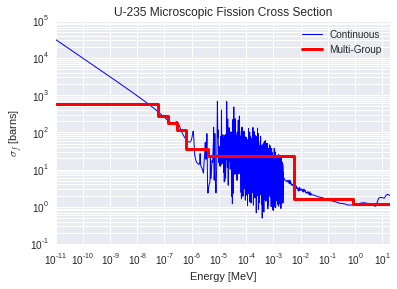
\includegraphics[width=0.8\linewidth]{figures/intro/u235-ce-mg-xs}
\caption[U-235 continuous energy and multi-group fission cross section]{U-235 continuous energy and 16-group fission cross section.}
\label{fig:chap1-u235-sigf}
\end{figure}

Many different engineering prescriptions have been developed to generate \ac{MGXS} for specific reactor configurations and spectra. In general, \ac{MGXS} generation schemes use a multi-level approach to decouple the energy, angular and spatial dimensions as depicted in Fig.~\ref{fig:chap1-multi-level-flow-chart}. The multi-level approach typically applies high-fidelity models of the energy self-shielding physics to low-fidelity geometric models of unique core components. The complexity of the energy treatment is then reduced at each level as larger and more complex geometric models are considered.

\begin{figure}
\centering
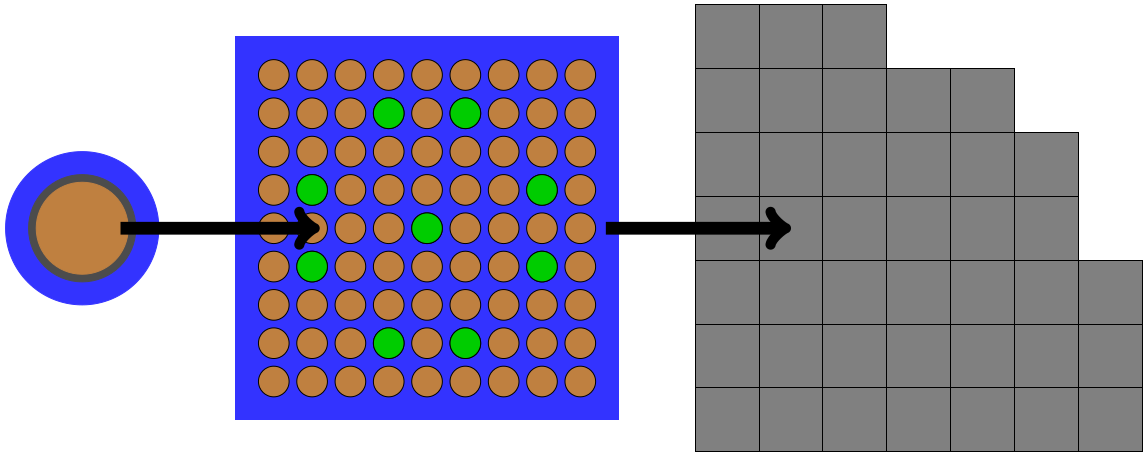
\includegraphics[width=0.9\linewidth]{figures/intro/multi-step-flow-chart}
\caption[Multi-level approach to reactor analysis]{Current multi-level framework for reactor analysis.}
\label{fig:chap1-multi-level-flow-chart}
\end{figure}

For example, the first stage for \ac{LWR} \ac{MGXS} generation attempts to capture energy self-shielding effects within simplified geometric models such as infinite fuel pin cells. This step typically condenses continuous energy cross sections to $\mathcal{O}(100)$ groups. These \ac{MGXS} are then used in a heterogenous lattice physics calculation of an individual fuel assembly within an infinite lattice. The lattice physics calculation models spatial self-shielding effects between pins of various material compositions and condenses the \ac{MGXS} to a coarse energy structure of $\mathcal{O}(10)$ groups. In addition, the \ac{MGXS} may be spatially-homogenized across the entire fuel assembly or across each fuel pin within each assembly. Finally, the spatially-homogenized coarse \ac{MGXS} for each fuel assembly are used in a whole-core calculation composed of many fuel assemblies.

The multi-level approach uses a combination of models of varying complexity to optimize overall simulation speed with accuracy. However, this is typically done at the sake of generality. For example, some prior knowledge of the neutron energy spectra is required to design approximations to the flux for a particular reactor configuration. Furthermore, multi-level \ac{MGXS} generation schemes do not generally model inter-assembly physics or the effect of reflectors and other core heterogeneities on the spatial distribution of the flux. Instead, geometric heuristcs are often used to embed spatial self-shielding effects in \ac{MGXS} for similarly shielded spatial zones (\textit{e.g.}, fuel pins). The approximations to the energy and spatial variation of the flux introduce approximation error in whole-core calculations and limit the space of core design parameters for which multi-level schemes may be applied. New reactor agnostic \ac{MGXS} generation methods are needed to enable deterministic transport-based methods to be as accurate and flexible as Monte Carlo in whole-core calculations.

%For reactors with a greater degree of spectral coupling, however, these approximations are not valid, resulting in ever larger datasets for the cross section generation process.

This thesis investigates the use of Monte Carlo methods to generate \ac{MGXS} for whole-core deterministic reactor analyis. Monte Carlo presents a natural approach to replace engineering prescriptions to approximate the flux with a stochastic approximation of the exact flux. The advantage of a \ac{MC}-based approach is that all of the relevant physics modeled in \ac{MC} may be directly embedded into \ac{MGXS}. This improvement in accuracy comes at the computational expense of converging group constant tallies to acceptably low uncertainties. \ac{MC} methods have increasingly been used to generate few group constants for coarse mesh diffusion, most notably by the Serpent \ac{MC} code~\cite{serpent2013manual}. However, there exist few rigorous and comprehensive analyses of \ac{MGXS} generation for heterogeneous fine mesh deterministic transport methods. 

\begin{emphbox}
\textbf{This thesis develops and evaluates \ac{MC}-based methods to generate \ac{MGXS} for fine mesh deterministic neutron transport codes.}
\end{emphbox}

In addition, \ac{MC}-based \ac{MGXS} generation methods to date have retained the multi-level geometric framework to tabulate \ac{MGXS} for individual reactor components -- such as infinite fuel pins and/or assemblies -- for subsequent use in whole-core multi-group calculations. Although the use of \ac{MC} within a multi-level scheme eliminates the need to approximate the flux in energy, it is does not account for spatial self-shielding effects throughout a reactor core. This thesis abandons the multi-level framework in place of a whole-core \ac{MC} calculation which simultaneously accounts for all energy and spatial self-shielding effects in a single step.

In theory, whole-core \ac{MC} calculations can be used to tally \ac{MGXS} in each spatial zone (\textit{e.g.}, 50,000+ fuel pins in a \ac{PWR} core) to account for the spatial variation in the flux. However, such simulations have not been employed for practical reasons -- in particular, the large memory footprint and computational expense of performing such calculations has been prohibitive for \ac{MC} codes until recent years. Furthermore, roughly the same number of particle histories would be required to converge the \ac{MGXS} tallies in each spatial zone as would be required for a direct whole-core calculation by \ac{MC}. Hence, it would be more useful to simply use \ac{MC} to compute the solution to the whole-core eigenvalue problem directly rather than use it to fully embed spatial self-shielding effects in \ac{MGXS} for deterministic transport codes. Therefore, in order for \ac{MC} to be practical for reactor agnostic fine mesh \ac{MGXS} generation, a new method is required to accelerate the convergence rate of the \ac{MGXS} tallies in each fine mesh region to a degree that is not possible for conventional whole-core Monte Carlo simulations. 

This thesis proposes to use statistical clustering methods to accelerate the convergence rate of whole-core \ac{MC} calculations for \ac{MGXS} generation. The novel approach developed in this work relies on the fact that many distinct spatial zones across a reactor core will experience similar if not identical spatial self-shielding effects, and therefore have similar if not identical \ac{MGXS}. The stochastic nature of \ac{MC} simulations will contribute statistical ``noise'' to the tally estimates for the \ac{MGXS}. As a result, the \ac{MGXS} estimates for similarly self-shielded spatial zones will form clusters which will converge as more particle histories are simulated. The goal of this thesis is to develop and apply algorithms to identify \ac{MGXS} clusters from ``noisy'' Monte Carlo tally data and to predict the true mean of each cluster prior to convergence. This methodology aims to generate \ac{MGXS} for deterministic neutron transport codes in a reactor agnostic and computationally efficient manner.

%The true mean of each cluster will then be used as the predicted estimate for the multi-group cross-section for each fine-mesh region in each cluster.

\begin{emphbox}
\textbf{This thesis uses statistical clustering algorithms to accelerate whole-core \ac{MC} calculations
which simultaneously model all energy- and spatial self-shielding effects for fine mesh \ac{MGXS} generation.}
\end{emphbox}


%%%%%%%%%%%%%%%%%%%%%%%%%%%%%%%%%%%%%%%%%%%%%%%%%%%%%%%%%%%%%%%%%%%%%%%%%%%%%%%
\section{Thesis Objectives}
\label{sec:chap1-objectives}

The subject matter of this thesis is organized along two main themes:

\begin{itemize}
\item \textbf{\textit{Approximation Error}} -- Quantify and diagnose approximation error(s) in \ac{MGXS} generated from \ac{MC} methods for simple heterogeous benchmark problems.
\item \textbf{\textit{Statistical Clustering}} -- Develop statistical clustering methods to accelerate the convergence rate of \ac{MGXS} on heterogeneous \ac{MC} tally meshes.
\end{itemize}

The first theme of this thesis rigorously assesses the efficacy of \ac{MGXS} generation with \ac{MC} for fine mesh transport calculations. Some of the approximations made by \ac{MC}-based \ac{MGXS} generation are quantified, including the energy- and spatial-dependence of condensed \ac{MGXS}. An in-depth analysis of systematic bias resulting from constant-in-angle total \ac{MGXS} is presented, along with a scheme based on \ac{SPH} factors to compensate for this loss in accuracy. 

The second theme of this thesis develops a new methodology to simultaneously capture local and global spatial self-shielding effects in \ac{MGXS} for whole-core calcuations. This scheme applies statistical clustering methods to accelerate the convergence rate of \ac{MGXS} tallied on fine, heterogeneous spatial meshes in Monte Carlo. The latent variable model which inspires the clustering paradigm is presented, along with a discussion of the implementation of a data pipeline to evaluate clustering algorithms for \ac{MGXS} generation. A series of increasingly complex heterogeneous benchmarks are modeled to empirically compare the accuracy and convergence rate of the approach with more traditional multi-level schemes for \ac{MC}-based MGXS generation.


%%%%%%%%%%%%%%%%%%%%%%%%%%%%%%%%%%%%%%%%%%%%%%%%%%%%%%%%%%%%%%%%%%%%%%%%%%%%%%%
\section{Thesis Outline}
\label{sec:chap1-outline}

This thesis is segmented into five Parts. Part I is comprised of this introductory chapter.

Part II discusses the relevant background information for this thesis. Chap.~\ref{chap:mgxs} reviews multi-group neutron transport theory and considers some common approximations made in \ac{MGXS} generation and multi-group transport codes. Chap.~\ref{chap:mgxs-mc} introduces Monte Carlo as an approach to generate \ac{MGXS}, and highlights relevant studies in the literature which have used \ac{MC} to generate \ac{MGXS}. Chap.~\ref{chap:workflow} presents the simulation workflow developed for this thesis to evaluate \ac{MC} for \ac{MGXS} generation, including the OpenMC, OpenMOC and OpenCG codes.

Part III diagnoses common sources of approximation error in \ac{MGXS} generation and multi-group transport methods. Chap. \ref{chap:biases} quantifies the impact of multi-group approxmation error for simple, heterogeneous \ac{PWR} geometries. Chap.~\ref{chap:sph} presents an algorithmic approach to mitigate systematic biases resulting from constant-in-angle total \ac{MGXS} using \ac{SPH} factors, and motivates the need for future work to address this issue.

Part IV develops a novel approach based on statistical clustering methods to accelerate whole-core \ac{MC} calculations for \ac{MGXS} generation. Chap.~\ref{chap:benchmarks} analyzes the convergence rate of \ac{MGXS} datasets computed on fine spatial \ac{MC} tally meshes for a series of heterogeneous \ac{PWR} benchmark models to motivate this new methodology. Chap.~\ref{chap:quantify} quantifies the impact of using \ac{MGXS} which reflect inter-pin and inter-assembly spatial self-shielding effects on the solutions computed by multi-group deterministic transport methods. Chap.~\ref{chap:spatial} analyzes the emergence of \ac{MGXS} clusters due to spatial self-shielding with a variety of visual aids. Chap.~\ref{chap:unsupervised} outlines a latent variable model for clustering \ac{MGXS}, along with a data pipeline for unsupervised clustering to accelerate the \ac{MGXS} convergence rate. Chapter~\ref{chap:results} evaluates the impact of clustered \ac{MGXS} on the accuracy and convergence rate of the eigenvalue solutions computed by deterministic transport methods.

Part V is composed of Chapter~\ref{chap:conclusions} which summarizes the progress made in this thesis to chart a path forward for \ac{MC}-based \ac{MGXS} generation for whole-core deterministic transport methods.

%\begin{figure}
%\begin{subfigure}{\textwidth}
%  \centering
%  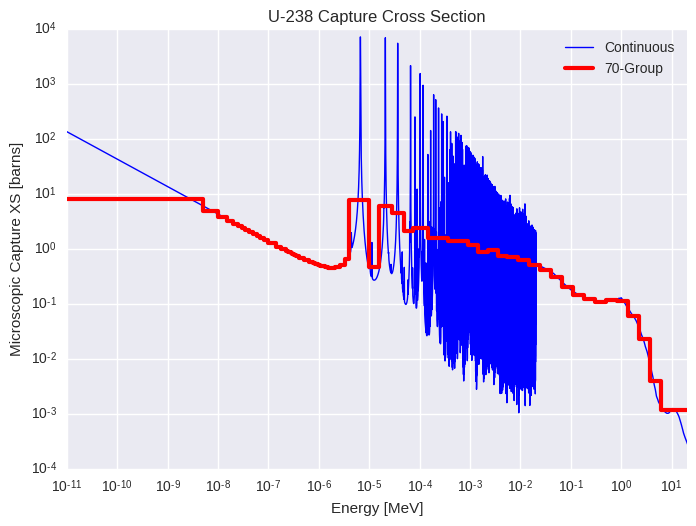
\includegraphics[width=0.9\linewidth]{figures/intro/u238-capture-70}
%  \caption{}
%\end{subfigure}
%\begin{subfigure}{\textwidth}
%  \centering
%  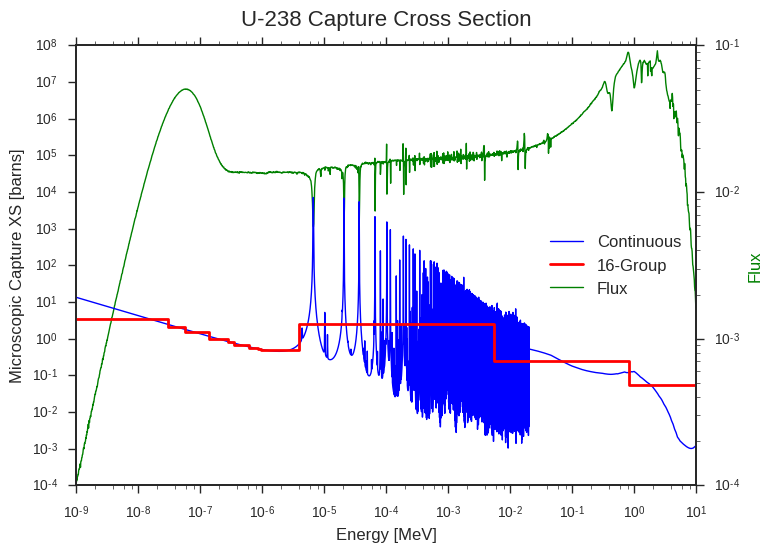
\includegraphics[width=0.9\linewidth]{figures/intro/u238-capture-16}
%  \caption{}
%\end{subfigure}
%\caption[Uranium-238 capture cross section]{Continuous energy and multi-group cross sections for U-238 capture in a PWR spectrum for 70-groups (a) and 16-groups (b).}
%\label{fig:pwr-ce-mg-xs}
%\end{figure}


%\chapter{Literature Review}
\label{chap:literature-review}

INTRO

%%%%%%%%%%%%%%%%%%%%%%%%%%%%%%%%%%%%%%%%%%%%%%%%%%%%%%%%%%%%%%%%%%%%%%%%%%%%%%%%
\section{2D/1D Methods}
\label{sec:2d_1d}
TODO

%%%%%%%%%%%%%%%%%%%%%%%%%%%%%%%%%%%%%%%%%%%%%%%%%%%%%%%%%%%%%%%%%%%%%%%%%%%%%%%%


%%%%%%%%%%%%%%%%%%%%%%%%%%%%%%%%%%%%%%%%%%%%%%%%%%%%%%%%%%%%%%%%%%%%%%%%%%%%%%%%
\section{3D MOC Implementations}
\label{sec:3d-imp}

3D MOC implementations

\section{The LEAF Method}
\label{sec:leaf}

A successor to the ASMOC3D method~\cite{pre_leaf}, the LEAF method~\cite{leaf_init, leaf_method} approaches the 3D \ac{MOC} problem in a very unique manner. Instead of basing the method on characteristic lines, vertically oriented characteristic planes are used instead. These methods ray traces over certain axial zones, much like a 2D/1D method, assuming an axially extruded geometry in which every radial plane has the same meshing. The vertically oriented characteristic planes are chosen to link at interfaces -- both between axial zones and between connecting planes along the same radial direction within the current axial zone. In the LEAF method, the angular flux at interfaces is represented with a 2nd order Legendre expansion.

The equations are cast in terms of collision probabilities, escape probabilities, and transmission probabilities for the planes. Numerical integration is applied for each characteristic plane in order to determine the these probabilities. This numerical integration is accomplished by laying axially stacked tracks across the plane for a given polar angle. These tracks form the abscissa of the integration. 

At this point, the method described is very similar to 3D \ac{MOC}. Aside from the angular flux being represented at interfaces by a 2nd order Legendre expansion, the numerical integration by laying axially stacked tracks in the plane causes the method to be equivalent to filling the geometry full of characteristic lines. It is essentially a re-working of the equations to cast the problem in a different context.

However, the main difference for practical application comes when these probabilities are computed as part of a pre-processing step. Rather than explicitly computing the probabilities (collision, escape, and transmission) of all vertical planes in the problem, the probabilities are computed and tabulated for a range of conditions and interpolated during transport sweeps. The interpolation parameters are: polar angle, axial height of the vertical plane, radial thickness, and total cross-section. By creating the lookup tables only using the chosen abscissa, the amount of work can be greatly reduced.

Since the goal of this method is to treat coarse axial regions, higher order source approximations are introduced. Specifically sources are formed up to 2nd order in the axial direction and first order in the radial direction. These higher order source approximations allow for a significantly coarsened mesh while maintaining accuracy, reducing the computational requirements of the method.

So far the method has only been tested on somewhat small problems. However, it shows great potential. As long as the required probabilities can be accurately interpolated from somewhat coarse abscissa and the 2nd order Legendre approximation of angular flux is sufficiently accurate, this method should outperform 3D \ac{MOC} methods. However, if a very large number of abscissa are required or the 2nd order Legendre approximation is not sufficient, then explicit 3D \ac{MOC} methods would be preferable. 

\subsection{DRAGON}
\label{sec:dragon}
DRAGON is a neutron transport code concentrating on lattice physics calculations for CANDU reactors. Since CANDU reactors contain fuel elements with reactivity control devices placed perpendicularly to the fuel channels, accurate calculations require full 3D treatment of the physics. Therefore, a 3D \ac{MOC} solver was implemented, named MCI~\cite{dragon_3d_moc}. 

MCI solves the flat source \ac{MOC} equations using a nested iterative process. In outer iterations, the fission source is updated along with the eigenvalue estimate. During inner iterations, the scattering source is updated and transport sweeps yield currents and fluxes. Outward currents are tallied at boundaries with an albedo boundary condition yielding new inward angular fluxes for the following inner iteration. Acceleration is provided with a self-collision rebalancing scheme in which the energy distribution is rebalanced on every inner iteration.

A track merging technique was also implemented in which tracks crossing the same regions in the same order are merged. While this may be useful for simple geometries, there would not be many tracks which have the same crossings in complex geometries. Typical full core problems have many radial complexities, reducing the effectiveness of this scheme.

Distributed memory parallelism was also introduced into MCI~\cite{dragon_parallel}. In the implementation, each process received a copy of all scalar fluxes and a group of tracks to handle. After completing each transport sweep, a global reduction communicated flux information through a sum operation on every region. Angular fluxes were also communicated through global broadcasts. In order to optimize load balancing, many partitioning schemes for the tracks across processes were tested. While the parallel efficiency was decent for the tested cases, the largest case only used 8 CPU cores. For the time of the tests, this was standard. However, for modern parallel computing, this number of cores is quite small, especially for large scale neutron transport calculations.

\subsection{MOCFE}
\label{sec:mocfe}

MOCFE is a finite element \ac{MOC} created at Argonne National Laboratory~\cite{mocfe_init}. Using a finite element approach, the \ac{MOC} system of equations with a flat source approximation were solved in matrix. The iteration scheme consisted of iterations over between group and within-group components. In this nested iteration scheme, the inner iterations iteratively converged the within-group flux solution. Each inner iteration is a transport sweep. Though this scheme is not unusual, it does increase the number of transport sweeps needed to converge the problem.

MOCFE also does not link tracks at boundaries. Due to this implementation decision, approximations are required to treat reflective or periodic boundary conditions. However, the lack of track linking requirements allows for less constraints when constructing a quadrature set. MOCFE implements a quadrature set such that the projection to the spherical harmonics of the scattering kernel are exactly preserved. Tracks are also created symmetric in $z$ with each track representing both forward and backward angular fluxes.

The parallelism in MOCFE is implemented with \ac{MPI}~\cite{mpi} parallel over trajectories such that each process receives a copy of all source regions. On every transport sweep, each process computes the variation of angular fluxes over its trajectories and accumulates their contribution to all source regions. In order to communicate the results, global reductions are required at the end of each transport sweep, which can be quite expensive.

Application of MOCFE to large scale problems distributed across many processors was studied at length~\cite{mocfe_bgp}. In order to increase scalability, the entire space, angle, and energy variables were decomposed across \ac{MPI} processes. While this does indeed increase the parallelism, it can lead to dramatically inefficient designs due to poor cache efficiency. In this thesis, energy groups for a given computation are always treated with the same core in order to increase performance.

The decision to explicitly store \ac{MOC} information in matrices can also lead to poor performance. Typical efficient \ac{MOC} implementations implicitly compute matrix elements of the transport equations on-the-fly rather than storing the data in some typical matrix representation.  MOCFE also uses a \ac{GMRES} linear solver to solve the \ac{MOC} equations. While \ac{GMRES} can be quite efficient for arbitrary matrices, the  \ac{MOC} application is quite unique in which matrices can be easily inverted in a transport sweep due to the matrix structure. A \ac{GMRES} implementation oblivious to this structure can incur significant overhead.

Since, the computational demands of MOCFE were too large in comparison with other neutron transport simulation tools, the 3D \ac{MOC} solver was abandoned when the code was merged into the PROTEUS neutron simulation suite. Instead of using a 3D \ac{MOC} solver, the code was re-purposed to solve the transport equations using 2D/1D methods in PROTEUS-MOC~\cite{proteus}.

\subsection{MMOC}
\label{sec:mmoc}

Liu created a 3D \ac{MOC} implementation based on modular ray tracing~\cite{liu_mrt} named MMOC. His track laydown algorithm, which allows natural track linking over modular domains, is used in this thesis and thoroughly discussed in Chapter~\ref{chap:track-laydown}. This track laydown is efficient with only slight adjustments needed from desired user parameters, allowing for greatly reduced computational costs in comparison with other track laydown methods which are less flexible and require extra tracks to be inserted in order to ensure track linking at boundaries~\cite{shaner-laydown}. By considering entire 2D cycle lengths rather than individual 2D track lengths when forming track linking relationships, the requirements are significantly less stringent, allowing for the added flexibility.

In this thesis, the modular ray tracing algorithm for track generation is useful for linking tracks at domain boundaries during domain decomposition across many nodes. However, Liu used the modular tracking mainly to reduce ray tracing costs. MMOC approaches the \ac{MOC} problem by splitting it into many modules. Over many of the modules, Liu notes that the geometry and track laydown are the same. Therefore, \textit{typical cells} are identified and ray tracing is only computed for unique cells. For applications in this thesis, ray tracing costs can be trivial in comparison with the overall work of solving the \ac{MOC} equations so the ray tracing aspect of MMOC is less applicable.

The MMOC implementation also allows for arbitrary order adjusted level symmetric quadratures. First, MMOC creates desired angles and ray spacing to accommodate a level-symmetric scheme. These desired values are then adjusted to ensure linking at module boundaries. Weights are also recalculated with the new angles.

MMOC was tested on a variety of problems and used \ac{CMFD} acceleration to reduce the number of required iterations to achieve convergence.  However, it appears that the algorithm was only tested on Cartesian problems, lacking any curved surfaces. Since reactor physics problems most commonly involve fuel pins which are cylindrical, these test problems were over-simplified. Since the Cartesian geometries can easily be decomposed into blocks, many having identical geometries, the reuse of ray tracing data would provide more benefit than expected on a realistic problem. Full core problems also typically have complex radial geometries, including such features as intermediate grid spacers, core baffles, and many curved surfaces. Therefore, the method of ray tracing only unique cells is not implemented in OpenMOC. However, the method for generating tracks to link at boundaries is quite useful.

\subsection{MPACT}
\label{sec:mpact}

Kochunas implemented a 3D \ac{MOC} solver in MPACT~\cite{mpact_initial, kochunas}, the standard neutron transport code in the VERA core simulator~\cite{vera}.  This was the first 3D \ac{MOC} solver implemented with the intention of solving full core PWR problems with full geometric detail. The solver used many of the common principles and structure of 2D \ac{MOC} solvers at the time. For instance, it used a flat source approximation and explicitly stored segment information during a pre-processing ray tracing step at the beginning of the solver. Unlike other solvers, it used a strict source iteration scheme without any inner iterations. 

The track laydown implemented in the 3D \ac{MOC} solver relied on the Modular Ray Tracing scheme~\cite{liu_mrt}. However, simplifications were made leading to the s-MRT method, discussed further in Chapter~\ref{chap:track-laydown}. One of the reasons presented for these simplifications was to avoid tracks intersecting corners. In OpenMOC, corner intersections are allowed and are explicitly treated. While the s-MRT method leads to a much simpler track laydown algorithm, it has serious drawbacks. Specifically, the axial ray spacing must be finer than the radial ray spacing. This is problematic for full core \ac{PWR} problems in which there is much greater geometric detail in the radial direction than the axial direction. This can lead to an artificial increase in the number of tracks required to resolve typical \ac{PWR} problems. Since the computational cost (both in memory usage and run time) scales linearly with the number of tracks, any large artificial increase in the number of tracks can significantly hinder the computational performance. Published MPACT results show only a modest artificial increase (~8\%) in the number of tracks, but a fine axial ray spacing was assumed to be necessary. Published results~\cite{shaner-laydown, openmoc-beavrs} for OpenMOC show that it is possible to significantly coarsen the axial ray spacing while maintaining solution accuracy.

One of the benefits of using a modular ray tracing track laydown is the ability to naturally link tracks at domain boundaries when using spatial domain decomposition. The 3D \ac{MOC} solver in MPACT implemented both spatial domain decomposition and angular domain decomposition using non-blocking \ac{MPI} communication~\cite{mpi}. For spatial domain decomposition, the geometry is decomposed into $N$ sub-domains where $N$ is equal to the number of \ac{MPI} processes per number of angular decompositions. An algorithm is implemented to subdivide the geometry in order to maximize the volume-to-surface area ratio of each sub-domain, reducing the relative communication costs which scale with surface area. For angular domain decomposition, each \ac{MPI} process, the scalar fluxes of the associated sub-domain are replicated, using global reductions to sum all of the tallied contributions to local scalar fluxes across all processes. This reduction operation was shown to be a bottleneck in the parallel scalability of the algorithm.

During each transport sweep, the sweeping algorithm first loops over energy groups, then over angles within the angular sub-domain, then over all tracks within the angular sub-domain in parallel using OpenMP. In this shared memory parallelism implementation, each thread receives a full copy of the scalar fluxes within the sub-domain. This replication of information allows contention between threads to be reduced, but also greatly increases the memory footprint of storing scalar fluxes. In addition, a reduction operation is required to sum together all of the local thread scalar fluxes.

%The choice to loop over energy groups on the outside (rather than on the inner-most loop) causes decreased vectorization. The choice to also loop over angles on the outside and only parallelize over tracks within an angle (rather than parallelizing over all tracks) reduces the potential for parallelism

During transport sweeps, each track represents both forward and backward directed angular fluxes, a common feature of 2D \ac{MOC} algorithms~\cite{kochunas2007twoway}. When computing the angular flux variation over each source region, the exponential computation is performed using a table interpolation.

\ac{CMFD} acceleration was implemented in MPACT using the \ac{GMRES} linear solver in PETSc with a block ILU preconditioner to solve the associated linear system. The solver was domain decomposed spatially and a procedure implemented to update angular fluxes at sub-domain boundaries~\cite{mpact_dd_cmfd}.

Various benchmarks were evaluated for the MPACT 3D \ac{MOC} solver. These benchmarks include the Takeda benchmark~\cite{takeda} and the C5G7 benchmark~\cite{c5g7}. Unfortunately, the results did not seem to match well with the reference solution. To understand performance on realistic \ac{PWR} problems, a realistic \ac{PWR} assembly was constructed and modeled. 

A theoretical computational performance model was developed which matched well with the observed computational performance of the MPACT 3D \ac{MOC} solver, showing a very high computational cost for full resolving a full core \ac{PWR} problem using the MPACT implementation of 3D \ac{MOC}.

\subsection{APOLLO3}
\label{sec:apollo3}

APOLLO3 is a nuclear reactor analysis code which recently incorporated a 3D \ac{MOC} solver named TDT~\cite{Sciannandrone2016}. TDT solves the \ac{MOC} equations in a nested iterative process, much like the MCI solver in DRAGON. However, TDT adds another layer of iterations. In the outer iterations, new fission sources are computed. Within each outer iteration, thermal iterations are performed in which the scattering source is recomputed. Within each thermal iteration, internal iterations are conducted in which the spatial distribution is resolved. These innermost iterations require computing transport sweeps at every step. This nested iterative process is not implemented in OpenMOC since it increases the number of transport sweeps per fission source calculation. 

One of the main differences between TDT and other \ac{MOC} solvers is the explicit treatment of boundaries. TDT classifies boundaries as open or closed. At open boundaries the angular flux is known. For example, at vacuum boundaries the incoming angular flux is known to be exactly zero. At closed boundaries, such as reflective or periodic boundaries, the angular flux is unknown. Whereas solvers such as OpenMOC treat closed boundaries by estimating the angular flux as being the value from the previous iteration, TDT explicitly computes the angular flux at boundaries by following tracks from an open boundary (where the angular flux is known) along a connecting cycle until it reflects onto the track of interest.

This boundary treatment is of course not possible if the geometry is encompassed entirely by closed boundaries. In these cases, TDT guesses an initial angular flux and follows the track cycle until the initial guess becomes mathematically irrelevant. It is unclear whether this is only implemented for cases with all closed boundaries or if this technique is used more generally.

Another critical feature of TDT is the \ac{CCM}. In this method, storage requirements are reduced by characterizing segments (or chords) into different groups: specifically horizontal, vertical, and mixed. For horizontal and vertical chords, their lengths can trivially be computed, and are referred to as \textit{recognized chords}. In addition, all recognized chords of the same type (horizontal or vertical) of the same region will have the same length. Some mixed chords may become recognized chords under certain circumstances, but it is far more difficult than horizontal or vertical chords. Chords that are not recognized chords are termed \textit{unrecognized chords}.

During an initial ray trace, the tracking information is compactly stored in Hit Surface Sequences, which only details the type of intersections a track observes. These sequences, which only consist of one integer per segment or chord, can determine both the type of intersections encountered (recognized or unrecognized) as well as the regions which the segments overlap.

For all unrecognized chords, segment lengths as well as exponential terms are computed and explicitly stored. During transport sweeps, they are simply loaded from memory. For all recognized chords, their segment lengths and exponential terms are computed on-the-fly during the transport sweeps with no upfront storage of segment information. Before the transport sweep an interpolation table is stored for the exponential term. During the transport sweep, this table is used for the computation of exponential terms for recognized chords. 

Some ideas of \ac{CCM} are implemented in OpenMOC. For instance, OpenMOC identifies vertical and horizontal chords in order to efficiently ray trace. However, other features of \ac{CCM} are not implemented. For instance, the effectiveness of the storage technique relies on many recognized chords. Many of the tests conducted on \ac{CCM} have a high ratio of axial source height to axial ray spacing, therefore having many recognized chords, and yielding favorable computational results. However, our previous tests have shown that for coarse axial source height, the axial ray spacing can also be coarsened, lowering the number of potential recognized chords.

%Adds "special directions" (completely vertical, completely horriztonal) to quadrature

%groups on outside

Initially, the TDT solver was dependent on a flat source approximation. Its accuracy was verified on a variety of benchmark problems~\cite{apollo3_3dmoc, apollo3_vv}. More recently, it has been extended to allow for axial polynomial expansions of the source~\cite{apollo3_extruded}. The radial variation of the neutron source within each source region is still assumed to be flat. The authors cite radial heterogeneity and complexity for not using a higher order source approximation in the radial plane. The higher order source approximation requires significantly more computational work per segment but allows a much coarser axial mesh to be used. \ac{CCM} is emphasized for its ability to mitigate the additional work required for the higher order source approximation as it allows for chords of equal lengths to be efficiently computed. While developed for arbitrary order axial polynomial expansions, the presentation focuses on quadratic axial sources.

The TDT implementation is parallelized with OpenMP. The work is divided in a task-based parallelism approach. Each thread receives a set of tracks and a full copy of the scalar flux accumulators. When a given thread changes angle, the local copy of scalar flux accumulators are synchronized with the global scalar flux accumulator. Since this synchronization can be a bottleneck for parallel scaling, tracks are sorted into groups to minimize the frequency of changing angle.

The TDT implementation has also recently extended its capabilities by adding $DP_n$ synthetic acceleration which supports polynomial flux fields~\cite{apollo3_exp}. This is perhaps the first publication of explicitly treating higher order source components with acceleration techniques. In OpenMOC, the higher order source components are not directly treated during acceleration. Instead, both flat and high order source components are updated together during the prolongation stage of the acceleration.

\subsection{CACTUS}
\label{sec:cactus}

CACTUS was one of the first developed 2D \ac{MOC} neutron transport simulators~\cite{cactus_2d}. It is part of the WIMS core physics simulator and has been the standard lattice physics code used by the simulator for over 20 years. Recently, a 3D \ac{MOC} solver named CACTUS3D was added~\cite{cactus_3d}, reusing much of the CACTUS code. 3D geometry and ray tracing abilities were added for CACTUS3D, with much of the framework of the flux solver imported from CACTUS. Since CACTUS3D observed significant changes in track laydown for small changes in tracking parameters, a new 3D \ac{MOC} solver was created as the main simulation tool in WIMS for solving core calculation~\cite{cactus_wims}. This solver, is named  CACTUSOT since rays are treated in a ``once-through'' approach.

In the once-through scheme, each track assumes zero incoming angular flux and is only followed until it reaches the boundary of the geometry. Therefore this approach is limited to core problems with vacuum boundaries. Since tracks do not pass their angular fluxes to other tracks, as would be the case in problems with reflected boundaries, a cyclic track laydown with track linking at boundaries does not need to be enforced. Instead, tracks are generated to uniformly fill the geometry. This is accomplished by generating parallel tracks at every angle on each boundary surface, separated by constant spacing in all directions. This approach was largely adopted due to concerns over untracked elements and calculation of element volumes.

Both CACTUS3D and CACTUSOT explicitly save tracking data for segments. Whereas CACTUS3D stores tracking information for \textit{every} segment, CACTUSOT uses a slice-based geometry treatment. In this approach, the geometry is split into different slices. Each slice represents the geometry over a certain axial interval. In common reactor problems there might only be a few to a several unique slices. Tracks are generated on each slice rather than the full problem and the tracking data is only stored for each unique slice. 

Since tracks are generated for each slice and are not guaranteed to align at slice interfaces, this creates an issue for determining the starting angular fluxes on slice interfaces. This is overcome by using track cross-sectional area and outward-directed angular fluxes to compute leakage rates out of the slices on each radial mesh cell on the interface boundary. Inward-directed angular fluxes are then computed by using tack cross-sectional areas and the computed leakage rates.

CACTUSOT also implements features found in CACTUS including \ac{CMFD} acceleration restricted to Cartesian mesh, treatments for both transport-corrected P0 and anisotropic P1 scatter, and a diamond difference representation of the neutron source along track segments. Parallelism is introduced with \ac{MPI} in which work is decomposed by track direction.

\subsection{TRRM}
\label{sec:trrm}

\subsection{Mockingbird}
\label{sec:mockingbird}

\part{Background}
\chapter{Transport Theory}
\label{chap:transport}

This chapter briefly introduces the fundamentals of neutron interactions in order to understand the origins of the neutron transport equation. First, neutron reactions are discussed in Section~\ref{sec:transport-fundamentals}, leading to a concise formula for their calculation in terms of the neutron population. Then, in Section~\ref{sec:transport-eq}, the sources and sinks of neutrons are identified in order to determine a general balance equation for the neutron population. Assumptions are then introduced and identified, leading finally to the multi-group transport equation, whose solution is the subject of this thesis. The emphasis in this description is identifying approximations and discussing their impact on solution accuracy. Other more traditional discussions of the neutron transport equation can be found throughout the literature~\cite{henry, duderstadt, duderstadt-martin, bell1967transport, hebert2009applied}. This thesis aims to form a cohesive description of steady-state neutron transport from fundamentals, mentioning all non-trivial approximations.

\section{Neutron Reactions}
\label{sec:transport-fundamentals}

The ultimate goal in neutron transport analysis is to determine the rates of neutron-induced reactions throughout the reactor core. Neutrons can induce or undergo various reactions when they strike materials existing in the reactor core, often referred to as \textit{target nuclei}. These interactions include scattering, capture, and fission, though others exist. Since neutrons are the initiators of these events, understanding their behavior is critical to determining the reaction rates.

The neutron population can be categorized by location $\mathbf{r}$, direction of travel $\mathbf{\Omega}$, and energy $E$ at each time $t$. Here, the bolding of variables differentiates scalar quantities (such as energy $E$) from vector quantities (such as direction $\mathbf{\Omega}$). Since neutrons modeled inside a nuclear reactor core exist far below the relativistic range, their energy $E$ can be directly related to their velocity $v$ as
\begin{equation}
E = \frac{1}{2} m_n v^2
\end{equation}
where $m_n$ is the mass of the neutron. Therefore, in the context of neutron transport, neutron velocity is nearly synonymous with neutron energy.

The reaction rate $R_X(\mathbf{r}, \mathbf{\Omega}, E, t)$ of type $X$ induced by neutrons of density $n(\mathbf{r}, \mathbf{\Omega}, E, t)$ striking a target material composed of $K$ isotopes, indexed by $k$, each with a number density of $\rho_k(\mathbf{r}, t)$ can be calculated as
\begin{equation}
R_X(\mathbf{r}, \mathbf{\Omega}, E, t) = \sum_{k=1}^K \sigma_{k,X}(\mathbf{r}, \mathbf{\Omega}, E, t) \rho_k(\mathbf{r}, t) n(\mathbf{r}, \mathbf{\Omega}, E, t) v(E) 
\label{eqn:rr_fundamental}
\end{equation}
where $\sigma_{k,X}(\mathbf{r}, \mathbf{\Omega}, E, t)$ is the microscopic nuclear cross-section of isotope $k$\cite{duderstadt}. The nuclear cross-section is a fundamentally important quantity in nuclear engineering that is often interpreted as the probability of a neutron interacting with the target nuclei. This particularly interesting material attribute is discussed further in Chapter~\ref{chap:mgxs}. For the purposes of this discussion on neutron transport, it is necessary to calculate reaction rates -- the goal of neutron transport calculations.

Notice that of the four components in Eq.~\ref{eqn:rr_fundamental}, the first two relate to the target material and the last two relate to the impinging neutrons. These terms are therefore grouped into the macroscopic nuclear cross-section $\Sigma_X(\mathbf{r}, \mathbf{\Omega}, E, t)$ defined as
\begin{equation}
\Sigma_X(\mathbf{r}, \mathbf{\Omega}, E, t) \equiv \sum_{k=1}^K \sigma_{k,X}(\mathbf{r}, \mathbf{\Omega}, E, t) \rho_k(\mathbf{r}, t)
\end{equation} 
and the neutron angular flux $\psi(\mathbf{r}, \mathbf{\Omega}, E, t)$ defined as
\begin{equation}
\psi(\mathbf{r}, \mathbf{\Omega}, E, t) \equiv n(\mathbf{r}, \mathbf{\Omega}, E, t) v(E).
\label{eqn:angular_neutron_flux}
\end{equation}
With these definitions, the reaction rates can be calculated simply as the product of macroscopic cross-section and angular neutron flux:
\begin{equation}
R_X(\mathbf{r}, \mathbf{\Omega}, E, t) = \Sigma_X(\mathbf{r}, \mathbf{\Omega}, E, t) \psi(\mathbf{r}, \mathbf{\Omega}, E, t).
\label{eqn:rr_differential}
\end{equation}

Often, integrated reaction rates over a region in space are desired. For instance, determining the fission reaction rate within a fuel rod dictates the amount of heat produced by the rod, a necessary input for thermal analysis of a reactor core. The time-dependent fission reaction rate $R_F(t)$ within a volume $V$ with macroscopic fission cross-section $\Sigma_f(\mathbf{r}, \mathbf{\Omega}, E, t)$ at time $t$ can be calculated by integrating Eq.~\ref{eqn:rr_differential} over the volume, all directions, and all energies:

\begin{equation}
R_{F}(t) = \int_{V} d\mathbf{r} \,  \int_{4\pi} d\mathbf{\Omega} \, \int_{0}^{\infty} dE \, \Sigma_f(\mathbf{r}, \mathbf{\Omega}, E, t) \psi(\mathbf{r}, \mathbf{\Omega}, E, t)
\label{eqn:rr_psi}
\end{equation}

With known macroscopic cross-sections, all reaction rates can be determined by obtaining the neutron angular flux.

\section{The Neutron Transport Equation}
\label{sec:transport-eq}

Now that the fundamentals of calculating reaction rates have been established, a balance equation must be formed in order to solve for the neutron angular flux distribution. First, consider the rate of change in neutron population in a given volume $V$ over time in terms of the neutron sources and neutron sinks:
\begin{equation}
\frac{\partial}{\partial t} \int_V d\mathbf{r} \, n(\mathbf{r},\mathbf{\Omega},E,t) = \text{sources} - \text{sinks}
\end{equation}
From Eq.~\ref{eqn:angular_neutron_flux}, this neutron density rate of change can be written in terms of the neutron angular flux. After re-arranging terms, this yields Eq.~\ref{eqn:nt_fundamentals_1}.
\begin{equation}
\int_V d\mathbf{r} \, \left( \frac{1}{v(E)} \frac{\partial}{\partial t} \psi(\mathbf{r},\mathbf{\Omega},E,t)\right) + \text{sinks} = \text{sources}.
\label{eqn:nt_fundamentals_1}
\end{equation}
Now, all the relevant neutron sources and neutron sinks must be identified. With no non-trivial exceptions, the neutron sources are identified as
\begin{equation}
\begin{split}
\text{sources} = \text{prompt fission} \, + \, & \text{in-scattering} \, +  \, \text{neutron influx} \, + \\ & \text{delayed neutron emission} \, + \, \text{external sources} \\
\end{split}
\end{equation}
The prompt fission term refers to neutrons that are emitted during fission reactions. During the fission process, the impingent neutron of direction $\mathbf{\Omega}$ and energy $E$ is modeled as briefly being joined with the target nucleus to form a \textit{compound nucleus}. Then, the compound nucleus breaks into several pieces, including fission products but also releasing some additional neutrons. The number of additional neutrons follows a stochastic process. In deterministic transport, only the mean is modeled so the average number of neutrons released from the fission process. This is nuclide-dependent but in order to model the transport through materials rather individual isotopes, an average number of neutrons released from fission in the material $\nu_p(\mathbf{r},\mathbf{\Omega}, E, t)$ is assumed for every fission event. Due to the compound nucleus model from quantum mechanics~\cite{compound-nucleus}, it is possible to assume that the direction and energy of released fission neutrons follow a prompt emission spectrum $\chi_p(\mathbf{r},\mathbf{\Omega}, E,t)$ that is independent of the impingent neutron direction and energy. Therefore, the overall fission rate at each location can be calculated by integrating the product of fission cross-section $\Sigma_f(\mathbf{r},\mathbf{\Omega}, E, t)$  and angular flux over all incoming directions and energies. The prompt emission spectrum is then applied to determine the rate of neutrons emitted at direction $\mathbf{\Omega}$ and energy $E$ as
\begin{equation}
\begin{split}
\text{prompt } & \text{fission} =  \\
 \int_V d\mathbf{r} \, & \chi_p(\mathbf{r}, \mathbf{\Omega}, E,t) \int\displaylimits_{0}^{\infty} dE' \, \int\displaylimits_{4\pi} d\mathbf{\Omega'} \, \nu_p(\mathbf{r},\mathbf{\Omega'}, E', t) \Sigma_f(\mathbf{r},\mathbf{\Omega'}, E', t) \psi(\mathbf{r},\mathbf{\Omega'}, E',t)
\end{split}
\end{equation}
In-scattering refers to neutrons that collide with a target nucleus and scatter into direction $\mathbf{\Omega}$ and energy $E$ from another direction and energy pair $\mathbf{\Omega'}$ and $E'$, respectively. Unlike the prompt fission source, the outgoing neutron direction and energy cannot be decoupled from the incoming direction and energy. This is because the scattering magnitude ($\mathbf{\Omega} \cdot \mathbf{\Omega'}$) is highly dependent on the incoming neutron energy. For instance, a neutron is likely to be deflected far less from a light target than a heavier target due to conservation of momentum \cite{duderstadt}. Additionally, high energy neutrons are unlikely to scatter to higher energies. Therefore, a scattering macroscopic cross-section governing the probability of this scattering process is defined in terms of both incoming and outgoing neutron directions and energies as $\Sigma_{s}(\mathbf{r}, \mathbf{\Omega'}\rightarrow \mathbf{\Omega},{E'\rightarrow E},t)$. Integrating over all possible incoming neutron directions and energies yields the in-scattering source term:
\begin{equation}
\text{in-scattering} = \int_V d\mathbf{r} \, \int\displaylimits_{0}^{\infty} dE' \, \int\displaylimits_{4\pi} \, d\mathbf{\Omega'} \Sigma_{s}(\mathbf{r}, \mathbf{\Omega'}\rightarrow \mathbf{\Omega},{E'\rightarrow E},t) \psi(\mathbf{r}, \mathbf{\Omega'},E', t)
\end{equation}
The neutron influx term refers to the rate of neutrons entering the volume $V$ from outside its boundary. A surface $S$ is defined that bounds the volume $V$ and has a surface normal vector $\mathbf{n}$. In this way, all neutrons impingent on the surface $S$ with their direction pointed towards the volume ($\mathbf{\Omega} \cdot \mathbf{n} < 0$) contribute to the neutron influx. In addition, since the rate depends on the velocity of neutrons across the surface, but our definition of angular neutron flux encompasses the neutron velocity in the direction of travel $\mathbf{\Omega}$, the dot product must be taken with the surface normal $\mathbf{n}$. This leads to the definition of the neutron influx as:
\begin{equation}
\text{neutron influx} = - \int_{S \cap \left(\mathbf{\Omega} \cdot \mathbf{n} < 0 \right)} dS \, \left(\mathbf{\Omega} \cdot \mathbf{n} \right) \psi(\mathbf{r}, \mathbf{\Omega}, E, t)
\label{eqn:neutron-influx}
\end{equation}
where the negation is due to the dot product $\left(\mathbf{\Omega} \cdot \mathbf{n} \right)$ being negative.

The delayed neutron emission term refers to neutrons emitted from isotopes formed by the fission process. Some fission products are radioactive and decay via neutron emission. These neutrons are often far lower in energy than prompt fission neutrons. For the purpose of this discussion, no assumptions are made about the form of delayed neutron source and is left as a general function:
\begin{equation}
\text{delayed neutron emission} = \int_V d\mathbf{r} \, D(\mathbf{r}, \mathbf{\Omega}, E, t)
\end{equation}
Lastly, neutrons can be released from external sources found within the reactor core. For instance, radioactive sources that emit neutrons are often placed in the core during startup. Similar to the delayed neutron source, no assumptions are made about the form of these external sources:
\begin{equation}
\text{external sources} = \int_V d\mathbf{r} \, S(\mathbf{r}, \mathbf{\Omega}, E, t)
\end{equation}
Now that all of the relevant sources have been identified, it is time to identify the neutron sinks. With few exceptions, the sinks are identified as:
\begin{equation}
\text{sinks} = \text{neutron leakage} \, + \, \text{all neutron interactions}
\end{equation}
The neutron leakage term refers to the loss of neutrons leaving the volume $V$. This is calculated very similar to neutron influx in Eq.~\ref{eqn:neutron-influx} but for neutrons pointed away from the volume ($\mathbf{\Omega} \cdot \mathbf{n} \geq 0$).
\begin{equation}
\text{neutron leakage} = \int_{S \cap \left(\mathbf{\Omega} \cdot \mathbf{n} \geq 0 \right)} dS \, \left(\mathbf{\Omega} \cdot \mathbf{n} \right) \psi(\mathbf{r}, \mathbf{\Omega}, E, t)
\label{eqn:neutron-leakage}
\end{equation}
Combining Eq.~\ref{eqn:neutron-leakage} and Eq.~\ref{eqn:neutron-leakage}, the net leakage can be calculated as
\begin{equation}
\text{net leakage} = \text{neutron leakage} - \text{neutron influx} = \int_{S} dS \, \left(\mathbf{\Omega} \cdot \mathbf{n} \right) \psi(\mathbf{r}, \mathbf{\Omega}, E, t)
\label{eqn:net-leakage-surf}
\end{equation}
where the two integrals can be combined because together they form a non-overlapping partition of $S$. Using Gauss divergence theorem, the net leakage term can be cast as a volume integral:
\begin{equation}
\text{net leakage} = \int_V d\mathbf{r} \, \mathbf{\Omega} \cdot \nabla \psi(\mathbf{r},\mathbf{\Omega},E,t)
\label{eqn:net-leakage}
\end{equation}
The last term that needs to be defined is for all neutron interactions within the volume $V$. Since the direction $\mathbf{\Omega}$ and energy $E$ are continuous variables, in order to conserve momentum and energy, an observable interaction must change the neutron direction and energy. Therefore any observable reaction should be regarded as a loss of neutron population traveling at the incoming direction and energy. A total cross-section $\Sigma_{t}(\mathbf{r},\mathbf{\Omega},E, t)$ is defined relating to the total probability of any interaction. Therefore the total number of interactions withing the volume can be calculated as
\begin{equation}
\text{all neutron interactions} = \int_V d\mathbf{r} \, \Sigma_{t}(\mathbf{r},\mathbf{\Omega},E, t)\psi(\mathbf{r},\mathbf{\Omega},E,t).
\label{eqn:total-interactions}
\end{equation}
Combining all of these terms, a neutron balance equation is formed in Eq.~\ref{eqn:first-balance}
\begin{equation}
\begin{split}
\int_V d\mathbf{r} \, \frac{1}{v(E)} \frac{\partial \psi(\mathbf{r},\mathbf{\Omega},E,t)}{\partial t} \, + \, \int_V d\mathbf{r} \, \mathbf{\Omega} \cdot \nabla \psi(\mathbf{r},\mathbf{\Omega},E,t) \, + \, \int_V d\mathbf{r} \, \Sigma_{t}(\mathbf{r},\mathbf{\Omega},E, t)\psi(\mathbf{r},\mathbf{\Omega},E,t)\\
  =  \, \int_V d\mathbf{r} \, \chi_p(\mathbf{r}, \mathbf{\Omega}, E,t) \int\displaylimits_{0}^{\infty} dE' \, \int\displaylimits_{4\pi} d\mathbf{\Omega'} \, \nu_p(\mathbf{r},\mathbf{\Omega'}, E', t) \Sigma_f(\mathbf{r},\mathbf{\Omega'}, E', t) \psi(\mathbf{r},\mathbf{\Omega'}, E',t )\\
 + \, \int_V d\mathbf{r} \, \int\displaylimits_{0}^{\infty} dE' \, \int\displaylimits_{4\pi} \, d\mathbf{\Omega'} \Sigma_{s}(\mathbf{r}, \mathbf{\Omega'}\rightarrow \mathbf{\Omega},{E'\rightarrow E},t) \psi(\mathbf{r}, \mathbf{\Omega'},E', t) \\ 
 + \, \int_V d\mathbf{r} \, S(\mathbf{r}, \mathbf{\Omega}, E, t) +  \int_V d\mathbf{r} \, D(\mathbf{r}, \mathbf{\Omega}, E, t)
\end{split}
\label{eqn:first-balance}
\end{equation}

Since the volume $V$ was defined arbitrarily and all terms are integrated over the volume, in order for the equality to hold the function must be identical across all possible volumes. This is only true if the underlying functions are identical. Therefore the integral can be dropped from all terms yielding a new balance equation in Eq.~\ref{eqn:first-diff-balance}.
\begin{equation}
	\begin{split}
		\frac{1}{v(E)} \frac{\partial \psi(\mathbf{r},\mathbf{\Omega},E,t)}{\partial t} \, & + \, \mathbf{\Omega} \cdot \nabla \psi(\mathbf{r},\mathbf{\Omega},E,t) \, + \, \Sigma_{t}(\mathbf{r},\mathbf{\Omega},E, t)\psi(\mathbf{r},\mathbf{\Omega},E,t) = \\
		& \phantom{+} \, \chi_p(\mathbf{r}, \mathbf{\Omega}, E,t) \int\displaylimits_{0}^{\infty} dE' \, \int\displaylimits_{4\pi} d\mathbf{\Omega'} \, \nu_p(\mathbf{r},\mathbf{\Omega'}, E', t) \Sigma_f(\mathbf{r},\mathbf{\Omega'}, E', t) \psi(\mathbf{r},\mathbf{\Omega'}, E',t )\\
		& + \, \int\displaylimits_{0}^{\infty} dE' \, \int\displaylimits_{4\pi} \, d\mathbf{\Omega'} \Sigma_{s}(\mathbf{r}, \mathbf{\Omega'}\rightarrow \mathbf{\Omega},{E'\rightarrow E},t) \psi(\mathbf{r}, \mathbf{\Omega'},E', t) \\ 
		& + \, S(\mathbf{r}, \mathbf{\Omega}, E, t) + D(\mathbf{r}, \mathbf{\Omega}, E, t).
	\end{split}
	\label{eqn:first-diff-balance}
\end{equation}
This is the time-dependent neutron transport equation. In the context of this thesis, only steady-state problems will be analyzed, removing any temporal dependence. Therefore all time-dependence can be eliminated from Eq.~\ref{eqn:first-diff-balance}. In doing so, the delayed neutron emission is encompassed by the fission emission term, yielding a new fission emission spectrum $\chi(\mathbf{r}, \mathbf{\Omega}, E)$ and a new average number of neutrons per fission $\nu(\mathbf{r}, \mathbf{\Omega}, E)$ in Eq~\ref{eqn:first-time-independent-balance}.
\begin{equation}
\begin{split}
\mathbf{\Omega} \cdot \nabla \psi(\mathbf{r},\mathbf{\Omega},E) \, + & \, \Sigma_{t}(\mathbf{r},\mathbf{\Omega},E)\psi(\mathbf{r},\mathbf{\Omega},E) = \\
& \phantom{+} \, \chi(\mathbf{r}, \mathbf{\Omega}, E) \int\displaylimits_{0}^{\infty} dE' \, \int\displaylimits_{4\pi} d\mathbf{\Omega'} \, \nu(\mathbf{r},\mathbf{\Omega'},E') \Sigma_f(\mathbf{r},\mathbf{\Omega'}, E') \psi(\mathbf{r},\mathbf{\Omega'}, E')\\
& + \, \int\displaylimits_{0}^{\infty} dE' \, \int\displaylimits_{4\pi} \, d\mathbf{\Omega'} \Sigma_{s}(\mathbf{r}, \mathbf{\Omega'}\rightarrow \mathbf{\Omega},{E'\rightarrow E}) \psi(\mathbf{r}, \mathbf{\Omega'},E') \\ 
& + \, S(\mathbf{r}, \mathbf{\Omega}, E)
\end{split}
\label{eqn:first-time-independent-balance}
\end{equation}

Next, external sources are often assumed to be trivial. During full power operation of a nuclear power reactor, this is indeed true. The fission source overwhelms any external neutron source. Once the external sources are removed it is clear that the trivial solution $\psi(\mathbf{r},\mathbf{\Omega},E) = 0$ is a solution, and might indeed be the only solution that solves the problem for the provided cross-sections. 

In reality, the cross-sections are far from known. Instead, there are feedback mechanisms that force them to vary based on the neutron population. For instance, an increase in neutron population would likely lead to an increase in temperature that often causes neutron absorption to increase. Since cross-sections at steady-state operation are not precisely known, there is numerical difficulty in demanding equilibrium between sinks and sources. Therefore, a scaling factor $k$ is introduced in Eq.~\ref{eqn:k-indroduction} that modifies the fission source. This additional degree of freedom allows for solutions of the neutron transport equation were the unscaled sources do not exactly match the sinks.
\begin{equation}
	\begin{split}
		\mathbf{\Omega} \cdot \nabla \psi(\mathbf{r},\mathbf{\Omega},E) \, + & \, \Sigma_{t}(\mathbf{r},\mathbf{\Omega},E)\psi(\mathbf{r},\mathbf{\Omega},E) = \\
		& \phantom{+} \, \frac{\chi(\mathbf{r}, \mathbf{\Omega}, E)}{k} \int\displaylimits_{0}^{\infty} dE' \, \int\displaylimits_{4\pi} d\mathbf{\Omega'} \, \nu(\mathbf{r},\mathbf{\Omega'}E') \Sigma_f(\mathbf{r},\mathbf{\Omega'}, E') \psi(\mathbf{r},\mathbf{\Omega'}, E')\\
		& + \, \int\displaylimits_{0}^{\infty} dE' \, \int\displaylimits_{4\pi} \, d\mathbf{\Omega'} \Sigma_{s}(\mathbf{r}, \mathbf{\Omega'}\rightarrow \mathbf{\Omega},{E'\rightarrow E}) \psi(\mathbf{r}, \mathbf{\Omega'},E')
	\end{split}
	\label{eqn:k-indroduction}
\end{equation}
A closer examination of the scaling factor $k$ shows it is an eigenvalue of the system. This will become more obvious when a system of equations is formed to solve the neutron transport equation. In simulating steady state behavior, the dominant mode is often desired. The eigenvalue $k$ relating to that dominant mode is termed the criticality of the reactor. Only an eigenvalue $k=1$ indicates that the reactor is \textit{critical} -- that neutron sources exactly match sinks. However, due to imperfect knowledge of the system and its constituent material cross-sections the eigenvalue is never exactly $k=1$ in practical applications.

%If this mode corresponds to $k>1$, then the reactor is termed to be super-critical, meaning that sources overpower the sinks for the provided reactor configuration and cross-sections. A value of $k = 1$ implies the reactor is operating at perfect steady-state conditions, and the reactor is termed to be critical. For a value of $k < 1$ the reactor is termed to be sub-critical.

In the fission source term, the fission emission spectrum $\chi(\mathbf{r}, \mathbf{\Omega}, E)$ dictates how neutrons are emitted from fission events. Since the energy of emitted neutrons is so large in comparison with typical neutron energies causing neutron emission, as well as compound nucleus creation, there is virtually no dependence on angle. Therefore, the emission is assumed to be isotropic, as presented in Eq.~\ref{eqn:tr-isotropic-emission}.
\begin{equation}
	\begin{split}
		\mathbf{\Omega} \cdot \nabla \psi(\mathbf{r},\mathbf{\Omega},E) \, + & \, \Sigma_{t}(\mathbf{r},\mathbf{\Omega},E)\psi(\mathbf{r},\mathbf{\Omega},E) = \\
		& \phantom{+} \, \frac{\chi(\mathbf{r},E)}{4\pi k} \int\displaylimits_{0}^{\infty} dE' \, \int\displaylimits_{4\pi} d\mathbf{\Omega'} \, \nu(\mathbf{r},\mathbf{\Omega'},E') \Sigma_f(\mathbf{r},\mathbf{\Omega'}, E') \psi(\mathbf{r},\mathbf{\Omega'}, E')\\
		& + \, \int\displaylimits_{0}^{\infty} dE' \, \int\displaylimits_{4\pi} \, d\mathbf{\Omega'} \Sigma_{s}(\mathbf{r}, \mathbf{\Omega'}\rightarrow \mathbf{\Omega},{E'\rightarrow E}) \psi(\mathbf{r}, \mathbf{\Omega'},E')
	\end{split}
	\label{eqn:tr-isotropic-emission}
\end{equation}

Next, angular dependence is removed from non-scattering cross-sections, as well as the mean number of neutrons released by fission $\nu(\mathbf{r},\mathbf{\Omega},E')$ in Eq.~\ref{eqn:xs-angular-dependence-removal}. Since materials with strong orientation structures (eg. a crystalline structure) are uncommon in typical reactor configurations, this assumption introduces virtually no bias.
\begin{equation}
	\begin{split}
		\mathbf{\Omega} \cdot \nabla \psi(\mathbf{r},\mathbf{\Omega},E) \, + & \, \Sigma_{t}(\mathbf{r},E)\psi(\mathbf{r},\mathbf{\Omega},E) = \\
		& \phantom{+} \, \frac{\chi(\mathbf{r},E)}{4\pi k} \int\displaylimits_{0}^{\infty} dE' \, \nu(\mathbf{r},E') \Sigma_f(\mathbf{r}, E') \int\displaylimits_{4\pi} d\mathbf{\Omega'} \,  \psi(\mathbf{r},\mathbf{\Omega'}, E')\\
		& + \, \int\displaylimits_{0}^{\infty} dE' \, \int\displaylimits_{4\pi} \, d\mathbf{\Omega'} \Sigma_{s}(\mathbf{r}, \mathbf{\Omega'}\rightarrow \mathbf{\Omega},{E'\rightarrow E}) \psi(\mathbf{r}, \mathbf{\Omega'},E')
	\end{split}
	\label{eqn:xs-angular-dependence-removal}
\end{equation}

Many neutron transport methods rely on solving Eq.~\ref{eqn:xs-angular-dependence-removal} as it only incorporates very mild assumptions. For instance, many Monte Carlo solvers implicitly solve the neutron transport equation in this form~\cite{mcnpx2003manual, serpent2013manual, openmc2016manual, bucholz1982scale}. However, this form is too general for many deterministic solvers to be feasible. One of the added complexities comes from the angular dependence of the scattering source.

For computational efficiency, the scattering is therefore assumed to be isotropic. This assumption, unlike many of the others in this section, does indeed incorporate a measurable bias. In typical LWRs, significant hydrogen is present which scatters neutrons preferentially in the forward direction, which is not captured with the isotropic scattering assumption. However, in Section~\ref{eqn:transport-correction}, an adjustment will be introduced to account for the discrepancy between isotropic and anisotropic scattering. With the isotropic scattering assumption, all neutron sources are be simulated as equal in all directions, as presented in Eq.~\ref{eqn:transport-isotropic}.
\begin{equation}
	\begin{split}
		\mathbf{\Omega} \cdot \nabla \psi(\mathbf{r},\mathbf{\Omega},E) \, + & \, \Sigma_{t}(\mathbf{r},E)\psi(\mathbf{r},\mathbf{\Omega},E) = \\
		& \phantom{+} \, \frac{\chi(\mathbf{r},E)}{4\pi k} \int\displaylimits_{0}^{\infty} dE' \, \nu(\mathbf{r},E') \Sigma_f(\mathbf{r}, E') \int\displaylimits_{4\pi} d\mathbf{\Omega'} \,  \psi(\mathbf{r},\mathbf{\Omega'}, E')\\
		& + \, \int\displaylimits_{0}^{\infty} dE' \,  \frac{\Sigma_{s}(\mathbf{r},{E'\rightarrow E})}{4\pi}\int\displaylimits_{4\pi} \, d\mathbf{\Omega'} \psi(\mathbf{r}, \mathbf{\Omega'},E')
	\end{split}
	\label{eqn:transport-isotropic}
\end{equation}

The only angular dependence of source terms in Eq.~\ref{eqn:transport-isotropic} are due to the angular flux. Therefore it is convenient to define the scalar flux as the integral of the angular flux over all directions in Eq.~\ref{eqn:scalar-flux}.
\begin{equation}
\phi(\mathbf{r}, E) = \int\displaylimits_{4\pi} d\mathbf{\Omega} \,  \psi(\mathbf{r},\mathbf{\Omega}, E).
\label{eqn:scalar-flux}
\end{equation}
With this definition, the balance equation can be written more succinctly in Eq.~\ref{eqn:pre-multigroup}.
\begin{equation}
	\begin{split}
		\mathbf{\Omega} \cdot \nabla \psi(\mathbf{r},\mathbf{\Omega},E) \, + & \, \Sigma_{t}(\mathbf{r},E)\psi(\mathbf{r},\mathbf{\Omega},E) = \\
		& \phantom{+} \, \frac{\chi(\mathbf{r},E)}{4\pi k} \int\displaylimits_{0}^{\infty} dE' \, \nu(\mathbf{r},E') \Sigma_f(\mathbf{r}, E') \phi(\mathbf{r}, E')\\
		& + \, \int\displaylimits_{0}^{\infty} dE' \,  \frac{\Sigma_{s}(\mathbf{r},{E'\rightarrow E})}{4\pi} \phi(\mathbf{r}, E')
	\end{split}
	\label{eqn:pre-multigroup}
\end{equation}

\section{Multi-Group Transport}

Similar to how angular dependence of the scattering source causes increased computational complexity for deterministic methods, the continuous energy nature of the neutron transport equation \textit{greatly} increases computational complexity. Therefore, many deterministic methods rely on a multi-group form of the neutron transport equation in which neutron populations are grouped into energy intervals or \textit{groups}.

To determine the neutron population within a given energy group $g$, Eq.~\ref{eqn:pre-multigroup} is integrated over the associated energy interval with minimum energy corresponding to $E_{g-1}$ and maximum energy corresponding to $E_{g}$ which leads to Eq.~\ref{eqn:energy-range-int-transport}.
\begin{equation}
\begin{split}
\mathbf{\Omega} \cdot \nabla \psi_g(\mathbf{r},\mathbf{\Omega}) \, + & \, \int_{E_{g-1}}^{E_{g}} dE \, \Sigma_{t}(\mathbf{r},E)\psi(\mathbf{r},\mathbf{\Omega},E) = \\
& \phantom{+} \, \int_{E_{g-1}}^{E_g} dE \, \frac{\chi(\mathbf{r},E)}{4\pi k} \int\displaylimits_{0}^{\infty} dE' \, \nu(\mathbf{r},E') \Sigma_f(\mathbf{r}, E') \phi(\mathbf{r}, E')\\
& + \, \int_{E_{g-1}}^{E_g} dE \, \int\displaylimits_{0}^{\infty} dE' \,  \frac{\Sigma_{s}(\mathbf{r},{E'\rightarrow E})}{4\pi} \phi(\mathbf{r}, E')
\end{split}
\label{eqn:energy-range-int-transport}
\end{equation}
where the multi-group angular flux $\psi_g(\mathbf{r},\mathbf{\Omega})$ is defined as
\begin{equation}
\psi_g(\mathbf{r},\mathbf{\Omega}) = \int_{E_{g-1}}^{E_g} dE \, \psi(\mathbf{r},\mathbf{\Omega},E).
\end{equation}
If the entire energy range $[0, \infty)$ is partitioned into $G$ non-overlapping energy intervals, yielding $G+1$ energy boundaries, then integrals over the entire range can be cast as the sum of integrals over each energy interval. This is introduced in Eq.~\ref{eqn:transport-group-introduction}.
\begin{equation}
\begin{split}
\mathbf{\Omega} \cdot \nabla \psi_g(\mathbf{r},\mathbf{\Omega}) \, + & \, \int_{E_{g-1}}^{E_g} dE \, \Sigma_{t}(\mathbf{r},E)\psi(\mathbf{r},\mathbf{\Omega},E) = \\
& \phantom{+} \, \int_{E_{g-1}}^{E_g} dE \, \frac{\chi(\mathbf{r},E)}{4\pi k} \sum_{g'=1}^G \left( \int\displaylimits_{E_{g'-1}}^{E_{g'}} dE' \, \nu(\mathbf{r},E') \Sigma_f(\mathbf{r}, E') \phi(\mathbf{r}, E') \right)\\
& + \, \int_{E_{g-1}}^{E_g} dE \, \sum_{g'=1}^G \left( \int\displaylimits_{E_{g'-1}}^{E_{g'}} dE' \,  \frac{\Sigma_{s}(\mathbf{r},{E'\rightarrow E})}{4\pi} \phi(\mathbf{r}, E') \right).
\end{split}
\label{eqn:transport-group-introduction}
\end{equation}
For convenience, the group-wise scalar flux $\phi_g(\mathbf{r})$ is defined in Eq.~\ref{eqn:multi-group-scalar-flux}.
\begin{equation}
\phi_g(\mathbf{r}) = \int_{E_{g-1}}^{E_g} dE \, \phi(\mathbf{r},E)
\label{eqn:multi-group-scalar-flux}
\end{equation}
and \textit{multi-group cross-sections} are defined in Eq.~\ref{eqn:multi-group-xs-definitions-first} -- Eq.~\ref{eqn:multi-group-xs-definitions-last}.
\begin{eqnarray}
\Sigma_{t}^g(\mathbf{r},\mathbf{\Omega}) = \frac{\int_{E_{g-1}}^{E_g} dE \, \Sigma_{t}(\mathbf{r},E)\psi(\mathbf{r},\mathbf{\Omega},E)}{\int_{E_{g-1}}^{E_g} dE \, \psi(\mathbf{r},\mathbf{\Omega},E)} 
\label{eqn:multi-group-xs-definitions-first}\\
\nu \Sigma_f^g\left(\mathbf{r}\right) = \frac{\int\displaylimits_{E_{g'-1}}^{E_{g'}} dE \, \nu(\mathbf{r},E) \Sigma_f(\mathbf{r}, E) \phi(\mathbf{r}, E)}{\int\displaylimits_{E_{g'-1}}^{E_{g'}} dE \, \phi(\mathbf{r}, E)} \\
\chi_g\left(\mathbf{r}\right) = \frac{\int\displaylimits_{E_{g'-1}}^{E_{g'}} dE \, \chi(\mathbf{r},E) \sum_{g'=1}^G \nu \Sigma_f^{g'}(\mathbf{r}) \phi_{g'}(\mathbf{r})}{\sum_{g=1}^G \nu \Sigma_f^{g}(\mathbf{r}) \phi_{g}(\mathbf{r})}
\end{eqnarray}
\begin{equation}
\begin{split}
\Sigma_{s}^{g' \rightarrow g}\left(\mathbf{r}\right) = \frac{\int_{E_{g-1}}^{E_g} dE \, \int\displaylimits_{E_{g'-1}}^{E_{g'}} dE' \,  \Sigma_{s}(\mathbf{r},{E'\rightarrow E}) \phi(\mathbf{r}, E') }{\int_{E_{g-1}}^{E_g} dE \, \phi(\mathbf{r},E)}
\end{split}
\label{eqn:multi-group-xs-definitions-last}
\end{equation}
Incorporating these definitions into the transport equation yields the \textit{multi-group transport equation} given in Eq.~\ref{eqn:full-multi-group-transport}.
\begin{equation}
\begin{split}
\mathbf{\Omega} \cdot \nabla \psi_{g}(\mathbf{r},\mathbf{\Omega}) & \, + \, \Sigma_t^{g}(\mathbf{r},\mathbf{\Omega}) \psi_{g}(\mathbf{r},\mathbf{\Omega}) =  \\
& \frac{1}{4 \pi} \left( \frac{\chi_{g}\left(\mathbf{r}\right)}{k} \sum_{g'=1}^{G} \nu_{g'}\left(\mathbf{r}\right) \Sigma_f^{g'}\left(\mathbf{r}\right) \phi_{g'}\left(\mathbf{r}\right) + \, \sum_{g'=1}^G \,  \Sigma_{s}^{g' \rightarrow g}\left(\mathbf{r}\right) \phi_{g'}(\mathbf{r}) \right)
\end{split}
\label{eqn:full-multi-group-transport}
\end{equation}
It is important to note that no assumptions were needed from the energy independent form in Eq.~\ref{eqn:pre-multigroup} to arrive at the multi-group transport equation in Eq.~\ref{eqn:full-multi-group-transport}. However, the expressions for multi-group cross-sections are dependent on either scalar flux $\phi(\mathbf{r}, E)$ or angular flux $\psi(\mathbf{r},\mathbf{\Omega},E)$ which are unknown. Therefore, approximations need to be made in order to determine appropriate values for multi-group cross-sections. This will be the subject of Chapter~\ref{chap:mgxs}.

\newpage
\vfill
\begin{highlightsbox}[frametitle=Highlights]
	\begin{itemize}
		\item By properly identifying sources and sinks of neutrons, a balance equation can be derived from fundamentals.
		\item After light approximations, sources are limited to scattering and fission. Sinks are limited to neutron interactions and net leakage.
		\item In order to model reactors with imperfect knowledge of cross-sections, the eigenvalue $k$ is introduced which scales the fission source, forcing equilibrium between sources and sinks.
		\item This multi-group transport equation removes dependence on the continuous energy variable, producing a balance equation for each energy interval which are inter-dependent.
		\item The derivation of the multi-group transport equation from a continuous energy form involves no additional approximations, but relies on knowing the final solution in order to obtain accurate multi-group cross-section values.
		\item For the purpose of this thesis, scattering is assumed to be isotropic which introduces significant bias. However, this bias is hoped to be overcome with an appropriate transport correction, discussed in Chapter~\ref{chap:mgxs}.
	\end{itemize}
\end{highlightsbox}
\vfill
\chapter{Approximations in Multi-Group Transport Theory}
\label{chap:mgxs}

This chapter presents an overview of some of the approximations made by methods which solve the multi-group form of the neutron transport equation. This chapter begins by reviewing the continuous energy steady-state neutron transport equation in Sec.~\ref{sec:chap2-background}. The following sections present simplifications to the angular (Sec.~\ref{sec:chap2-approx-angle}), energy (Sec.~\ref{sec:chap2-approx-energy}) and spatial dependence (Sec.~\ref{sec:chap2-approx-space}) of the equation. The approximations introduced here are not specific to a particular approach for solving the transport equation and may be employed by either stochastic or deterministic methods. Sec.~\ref{sec:chap2-mgxs-lib} concludes with a discussion of how these approximations present challenges for accurate \ac{MGXS} generation.


%%%%%%%%%%%%%%%%%%%%%%%%%%%%%%%%%%%%%%%%%%%%%%%%%%%%%%%%%%%%%%%%%%%%%%%%%%%%%%%
\section{Background}
\label{sec:chap2-background}

The field of reactor physics is concerned with computing the distribution of nuclear reaction rates throughout a nuclear reactor core. Nuclear reaction rates are dependent on two fundamental quantities: the density of neutrons and the probability of interaction. The angular neutron flux $\psi(\mathbf{r},\mathbf{\Omega},E)$ models the neutron density\footnote{Unlike the common definition of flux used in other areas of science and engineering, the angular flux $\psi$ is the product of the volume density and speed of neutrons in phase space.} as the path length traveled by neutrons per unit volume and is dependent on a neutron's spatial position $\mathbf{r}$, direction of motion $\mathbf{\Omega}$ and energy $E$\footnote{This thesis focuses on steady-state calculations and time dependence is neglected for simplicity.}$^{,}$\footnote{Vector-valued quantities are expressed in boldface font.}. The macroscopic cross section $\Sigma_{x}(\mathbf{r},E)$ is defined as the probability of interaction $x$ per unit of length travelled by a neutron at some position and energy. A reaction rate $\mathcal{R}_{x}$ can be simply computed as the product of the angular flux and cross section:

\begin{dmath}
\label{eqn:chap2-rxn-rates}
\mathcal{R}_{x}(\mathbf{r},\mathbf{\Omega},E) = \Sigma_{x}(\mathbf{r},E) \psi(\mathbf{r},\mathbf{\Omega},E)
\end{dmath}

The macroscopic cross section $\Sigma$ is proportional to a quantity known as the microscopic cross section $\sigma_{x}$. The microscopic cross section is a property of a particular nuclide and is measured experimentally for various reaction types which include fission $f$, radiative capture $\gamma$ and scattering $s$\footnote{Scattering as defined here includes both inelastic and elastic scattering.}. The macroscopic cross section is the sum of the microscopic cross sections of each nuclide $i$ weighted by its number density $N_{i}$:

\begin{dmath}
\label{eqn:chap2-macro-xs-sum}
\Sigma_{x}(\mathbf{r},E) = \sum_{i}N_{i}(\mathbf{r})\sigma_{i,x}(E)
\end{dmath}

The microscopic cross section is highly dependent on the energy of the incoming neutron. As illustrated in see Fig.~\ref{fig:chap2-u238-xs}, a cross section may vary several orders of magnitude near resonances which may span only a few eV. The probability of some interactions also depend on other properties which characterize the output channel of the reaction. For example, the scattering cross section $\sigma_{s}$ depends on the energy and direction of motion of the outgoing neutron. The macroscopic cross section varies in space when nuclide densities depend on the position within a heterogeneous system.

\begin{figure}[H]
  \centering
  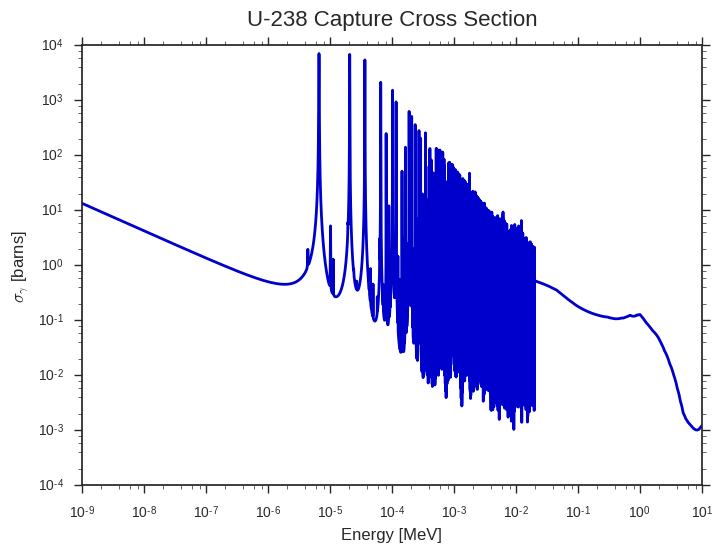
\includegraphics[width=0.8\linewidth]{figures/mgxs/u238-capture-xs}
\caption[U-238 capture cross section]{The continuous energy capture cross section for U-238.}
\label{fig:chap2-u238-xs}
\end{figure}
 
Although cross sections are experimentally measured, the neutron flux must be calculated analytically or with simulation. The steady-state Boltzmann transport equation~\cite{bell1970nuclear} is integro-differential in the neutron angular flux $\psi(\mathbf{r},\mathbf{\Omega},E)$ and balances the rate of change of the population of neutrons in phase space to the difference between the production and loss rates of neutrons within a closed system:

\begin{dmath}
\label{eqn:chap2-transport-ce}
\mathbf{\Omega} \cdot \nabla \psi(\mathbf{r},\mathbf{\Omega},E) + \Sigma_{t}(\mathbf{r},E)\psi(\mathbf{r},\mathbf{\Omega},E) \;\;\;\;\; = \;\;\;\;\; \int\displaylimits_{0}^{\infty}\int\displaylimits_{4\pi} \Sigma_{s}(\mathbf{r},{\mathbf{\Omega'}\rightarrow\mathbf{\Omega}},{E'\rightarrow E}) \psi(\mathbf{r},\mathbf{\Omega'},E') \mathrm{d}\mathbf{\Omega'} \mathrm{d}E' + Q(\mathbf{r},\mathbf{\Omega},E)
\end{dmath}

The first term on the left hand side of the equation represents the streaming of neutrons within space and the second term is the total neutron collision rate determined by the total cross section $\Sigma_{t}$. On the right hand side, the first term models the scattering of neutrons at some energy $E'$ and direction $\mathbf{\Omega'}$ into energy $E$ and direction $\mathbf{\Omega}$. The final term represents a generic source $Q$ of neutrons. In the case of critical systems, such as nuclear reactors, $Q$ is a source of fission neutrons:

\begin{dmath}
\label{eqn:chap2-source}
Q(\mathbf{r},\mathbf{\Omega},E) = \frac{1}{k_{eff}}\int\displaylimits_{0}^{\infty}\int\displaylimits_{4\pi} \nu\Sigma_{f}(\mathbf{r},{\mathbf{\Omega'}\rightarrow \mathbf{\Omega}},{E'\rightarrow E})\psi(\mathbf{r},\mathbf{\Omega'},E') \mathrm{d}\mathbf{\Omega'} \mathrm{d}E'
\end{dmath}

The fission production cross section $\nu\Sigma_{f}$ represents the probability of neutrons emitted at energy $E$ and angle $\mathbf{\Omega}$ resulting from fission events precipitated by neutrons at $E'$ and $\mathbf{\Omega'}$. The eigenvalue $k_{eff}$ of a critical system represents the multiplication of neutrons from fission and forces balance between neutron sources and losses due to absorption and leakage.

A solution for the neutron flux must computed from the transport equation in order to compute reaction rate distributions. The accurate determination of the neutron flux is primarily challenged by  the complicated energy structure of the cross sections. In addition, the distribution of neutrons in \ac{LWRs} spans 11 orders of magnitude from a few MeV at birth from fission emission to death by absorption at energies approaching 10$^{-5}$ eV. As a result, analytical solutions to Eqn.~\ref{eqn:chap2-transport-ce} are intractable without significant simplifying assumptions.

Instead, numerical simulation is used to solve the transport equation for the flux. Monte Carlo may be employed to exactly treat the energy dependence in Eqn.~\ref{eqn:chap2-transport-ce}\footnote{The treatment is only as exact as the uncertainties in measured nuclear cross section data will permit.}, but it is computationally burdensome and impractical for routine nuclear reactor analysis. Although space and angle may be discretized using standard techniques for the solution of PDEs, special treatment must be given to the energy variable. The following sections introduce approximations used to reduce the dimensionality of the equation to permit tractable multi-group calculations.

%The following sections present standard approximations made in multi-group theory to reduce the dimensionality of the angular, energy and spatial variables 


%%%%%%%%%%%%%%%%%%%%%%%%%%%%%%%%%%%%%%%%%%%%%%%%%%%%%%%%%%%%%%%%%%%%%%%%%%%%%%%
\section{Approximations in Angle}
\label{sec:chap2-approx-angle}

%%%%%%%%%%%%%%%%%%%%%%%%%%%
\subsection{Isotropic Fission Source}
\label{subsec:chap2-fiss-src}

The neutrons emitted from fission form a nearly isotropic distribution independent of the energy or angle of the incoming neutron. As a result, the fission production cross section can be approximated as $\nu\Sigma_{f}(\mathbf{r},{\mathbf{\Omega'}\rightarrow \mathbf{\Omega}},{E'\rightarrow E}) \approx \nu\Sigma_{f}(\mathbf{r},{E'\rightarrow E})$. This permits the fission source in Eqn.~\ref{eqn:chap2-source} to be written as:

\begin{dmath}
\label{eqn:chap2-source-scalar-flux}
Q(\mathbf{r},\mathbf{\Omega},E) = \frac{1}{4\pi k_{eff}}\int\displaylimits_{0}^{\infty}\int\displaylimits_{4\pi} \nu\Sigma_{f}(\mathbf{r},{E'\rightarrow E})\psi(\mathbf{r},\mathbf{\Omega'},E') \mathrm{d}\mathbf{\Omega'} \mathrm{d}E'
\end{dmath}

This expression may be further simplified in terms of the scalar neutron flux $\phi(\mathbf{r},E)$:

\begin{dmath}
\label{eqn:chap2-source-scalar-flux}
Q(\mathbf{r},\mathbf{\Omega},E) = \frac{1}{4\pi k_{eff}} \int\displaylimits_{0}^{\infty}\nu\Sigma_{f}(\mathbf{r},{E'\rightarrow E})\phi(\mathbf{r},E') \mathrm{d}E'
\end{dmath}

\begin{dmath}
\label{eqn:chap2-scalar-flux}
\phi_{g}(\mathbf{r},E) = \int\displaylimits_{4\pi}\psi(\mathbf{r},\mathbf{\Omega},E)\mathrm{d}\mathbf{\Omega}
\end{dmath}

The isotropic approximation reduces the dimensionality of the fission production term in the transport equation and simplifies the derivation of the approximations in the following sections.


%%%%%%%%%%%%%%%%%%%%%%%%%%%%%%
\subsection{Angular Expansion of the Scattering Kernel}
\label{subsec:chap2-scatt-src}

Unlike the fission source, the scattering source cannot be treated as isotropic since it is strongly dependent on the relationship between the incoming and outgoing directions of motion. The dimensionality of the scattering source term in the transport equation -- known as the double differential scattering kernel -- is commonly reduced with basis function expansions in angle~\cite{hebert2009applied, cacuci2010handbook}. The angular flux is first expanded as an infinite sum of spherical harmonic functions $Y_{\ell}^{m}(\mathbf{\Omega})$ and angular flux moments $\psi_{\ell}^{m}(\mathbf{r},E)$:

\begin{dmath}
\label{eqn:chap2-flux-expand}
\psi(\mathbf{r},\mathbf{\Omega},E) = \displaystyle\sum\limits_{\ell=0}^{\infty} \frac{2\ell+1}{4\pi} \displaystyle\sum\limits_{m=-\ell}^{\ell} \psi_{\ell}^{m}(\mathbf{r},E)Y_{l}^{m}(\mathbf{\Omega})
\end{dmath}

\begin{dmath}
\label{eqn:chap2-flux-moment}
\psi_{\ell}^{m}(\mathbf{r},E) = \displaystyle\int\limits_{4\pi} \psi(\mathbf{r},\mathbf{\Omega},E)Y_{\ell}^{m}(\mathbf{\Omega}) \mathrm{d}\mathbf{\Omega}
\end{dmath}

Similarly, the angular dependence of the scattering cross section $\Sigma_{s}(\mathbf{r},{\mathbf{\Omega'}\rightarrow\mathbf{\Omega}},{E'\rightarrow E})$ can be treated with a basis function expansion. The scattering cross section can be simplified without approximation by noting that the distribution over the change in direction $\mu$ is independent of the incoming angle $\mathbf{\Omega'}$ in isotropic media. The re-parametrized scattering cross section $\Sigma_{s}(\mathbf{r},\mu,E'\rightarrow E)$ can then expanded as an infinite sum of Legendre polynomials $P_{\ell}(\mu)$ and scattering moments $\Sigma_{s,\ell}(\mathbf{r},{E'\rightarrow E})$:

\begin{dmath}
\label{eqn:chap2-scatt-expand}
\Sigma_{s}(\mathbf{r},\mu,E'\rightarrow E) = \displaystyle\sum\limits_{\ell=0}^{\infty} \frac{2\ell+1}{2} \Sigma_{s,\ell}(\mathbf{r},{E'\rightarrow E})P_{\ell}(\mu)
\end{dmath}

\begin{dmath}
\label{eqn:chap2-scatt-moment}
\Sigma_{s,\ell}(\mathbf{r},E'\rightarrow E) = \displaystyle\int\limits_{-1}^{1} \Sigma_{s}(\mathbf{r},\mu,{E'\rightarrow E})P_{\ell}(\mu)\mathrm{d}\mu
\end{dmath}

The expansions of the angular flux in spherical harmonics and the scattering cross section in Legendre polynomials may be substituted into the scattering kernel. The spherical harmonic addition theorem can be applied to simplify the kernel in terms of only the real components $R_{\ell}^{m}(\mathbf{\Omega})$ of the spherical harmonics:

\begin{dmath}
\label{eqn:chap2-scatt-src-expand}
\int\displaylimits_{0}^{\infty}\int\displaylimits_{4\pi} \Sigma_{s}(\mathbf{r},{\mathbf{\Omega'}\rightarrow\mathbf{\Omega}},{E'\rightarrow E}) \psi(\mathbf{r},\mathbf{\Omega'},E') \mathrm{d}\mathbf{\Omega'} \mathrm{d}E' = \int\displaylimits_{0}^{\infty} \displaystyle\sum\limits_{\ell=0}^{\infty} \frac{2\ell+1}{4\pi} \Sigma_{s,\ell}(\mathbf{r},{E'\rightarrow E}) \psi_{\ell}^{m}(\mathbf{r},E')R_{\ell}^{m}(\mathbf{\Omega}) \mathrm{d}E'
\end{dmath}

No approximation has been made to the scattering kernel's angular dependence in Eqn.~\ref{eqn:chap2-scatt-src-expand}. In practice, however, the expansion is truncated to a finite number of spherical harmonics $L$ to make the transport equation computationally tractable. The transport equation with the scattering source expansion and isotropic fission source is then:

\begin{dmath}
\label{eqn:chap2-transport-ce-2}
\mathbf{\Omega} \cdot \nabla \psi(\mathbf{r},\mathbf{\Omega},E) + \Sigma_{t}(\mathbf{r},E)\psi(\mathbf{r},\mathbf{\Omega},E) = \int\displaylimits_{0}^{\infty} \displaystyle\sum\limits_{\ell=0}^{L} \frac{2\ell+1}{4\pi} \displaystyle\sum\limits_{m=-\ell}^{\ell} \Sigma_{s,\ell}(\mathbf{r},{E'\rightarrow E}) \psi_{\ell}^{m}(\mathbf{r},E')R_{\ell}^{m}(\mathbf{\Omega}) \mathrm{d}E' + \frac{1}{4\pi k_{eff}}\int\displaylimits_{0}^{\infty} \nu\Sigma_{f}(\mathbf{r},{E'\rightarrow E})\phi(\mathbf{r},E')\mathrm{d}E'
\end{dmath}


%%%%%%%%%%%%%%%%%%%%%%%%%%%%%%
\subsection{Transport Correction}
\label{subsec:chap2-transport-corr}

The scattering matrix and flux moments substantially increase the memory and storage requirements for calculation schemes which model anisotropic scattering with a finite moment expansion as introduced in Sec.~\ref{subsec:chap2-scatt-src}. In practice, many methods attempt to implicitly model anisotropic scattering effects with transport corrected cross sections. These approaches seek to define a correction which makes the transport equation with isotropic scattering in the laboratory system ($L=0$) equivalent to the general equation with anisotropic scattering. Various transport corrections are thoroughly detailed in \cite{macfarlane1993transx,macfarlane2000njoy}, each of which follow~\cite{bell1967transport}. This section summarizes the analysis in~\cite{hebert2009applied}.

First, consider a truncated form of the Legendre polynomial expansion of the scattering cross section $\Sigma_{s}(\mathbf{r},\mu,E'\rightarrow E)$ in Eqn.~\ref{eqn:chap2-scatt-expand}:

\begin{dmath}
\label{eqn:chap2-scatt-expand-truncate}
\Sigma_{s}(\mathbf{r},\mu,E'\rightarrow E) = \displaystyle\sum\limits_{\ell=0}^{\infty} \frac{2\ell+1}{2} \Sigma_{s,\ell}(\mathbf{r},{E'\rightarrow E})P_{\ell}(\mu) \approx \displaystyle\sum\limits_{\ell=0}^{L} \frac{2\ell+1}{2} \hat{\Sigma}_{s,\ell}(\mathbf{r},{E'\rightarrow E})P_{\ell}(\mu) + \Delta\Sigma_{tr}(\mathbf{r},{E'\rightarrow E})\delta(\mu-1)
\end{dmath}

where $\hat{\Sigma}_{s,\ell}$ is a modified form of the scattering moment $\Sigma_{s,\ell}$ and $\Delta\Sigma_{tr}$ is a transport correction term. The Kronecker delta function $\delta(\mu-1)$ is used to make the correction term forward peaked in order to best capture the first order anisotropies in thermal reactors. The coefficients $\hat{\Sigma}_{s,\ell}$ and $\Delta\Sigma_{tr}$ are defined such that the Legendre moments of the scattering cross section in Eqn.~\ref{eqn:chap2-scatt-moment} are preserved for $0 \le \ell \le L+1$:

\begin{dmath}
\label{eqn:chap2-scatt-moment-preserve}
\Sigma_{s,\ell}(\mathbf{r},E'\rightarrow E) = \displaystyle\int\limits_{-1}^{1} \Sigma_{s}(\mathbf{r},\mu,{E\rightarrow E})P_{\ell}(\mu)\mathrm{d}\mu \approx \displaystyle\int\limits_{-1}^{1} \displaystyle\sum\limits_{\ell'=0}^{L} \frac{2\ell'+1}{2} \hat{\Sigma}_{s,\ell'}(\mathbf{r},{E'\rightarrow E})P_{\ell'}(\mu)P_{\ell}(\mu)\mathrm{d}\mu + \displaystyle\int\limits_{-1}^{1} \Delta\Sigma_{tr}(\mathbf{r},{E'\rightarrow E})\delta(\mu-1)P_{\ell}(\mu)\mathrm{d}\mu
\end{dmath}

The following simultaneous system of equalities for $0 \le \ell \le L$ follows from the identity $P_{\ell}(1) = 1$ and the orthogonality relation of the Legendre polynomial basis set:

\begin{dmath}
\label{eqn:chap2-sigsl}
\hat{\Sigma}_{s,\ell}(\mathbf{r},{E'\rightarrow E}) + \Delta\Sigma_{tr}(\mathbf{r},{E'\rightarrow E}) = \Sigma_{s,\ell}(\mathbf{r},{E'\rightarrow E})
\end{dmath}

\begin{dmath}
\label{eqn:chap2-delta-transport}
\Delta\Sigma_{tr}(\mathbf{r},{E'\rightarrow E}) = \Sigma_{s,L+1}(\mathbf{r},{E'\rightarrow E})
\end{dmath}

For isotropic in lab scattering with $L = 0$ the Eqns.~\ref{eqn:chap2-scatt-expand-truncate} and~\ref{eqn:chap2-delta-transport} simplify in terms of only the zeroth and first order scattering moments:

\begin{dmath}
\label{eqn:chap2-iso-scatt-kernel-transport}
\Sigma_{s}(\mathbf{r},\mu,E'\rightarrow E) \approx \frac{1}{2}\left[\Sigma_{s,0}(\mathbf{r},{E'\rightarrow E}) - \Sigma_{s,1}(\mathbf{r},{E'\rightarrow E})\right] + \Sigma_{s,1}(\mathbf{r},{E'\rightarrow E})\delta(\mu-1)
\end{dmath}

The transport corrected scattering cross section in Eqn.~\ref{eqn:chap2-iso-scatt-kernel-transport} is then substituted into the transport equation in Eqn.~\ref{eqn:chap2-transport-ce-2} with an isotropic scattering kernel and rearranged to produce:

\begin{dmath}
\label{eqn:chap2-transport-ce-3}
\mathbf{\Omega} \cdot \nabla \psi(\mathbf{r},\mathbf{\Omega},E) + \Sigma_{t}(\mathbf{r},E)\psi(\mathbf{r},\mathbf{\Omega},E) - \int\displaylimits_{0}^{\infty} \Sigma_{s,1}(\mathbf{r},{E'\rightarrow E})\phi(\mathbf{r},E')\mathrm{d}E' = \frac{1}{4\pi} \int\displaylimits_{0}^{\infty} \left[\Sigma_{s,0}(\mathbf{r},{E'\rightarrow E}) - \Sigma_{s,1}(\mathbf{r},{E'\rightarrow E})\right] \phi(\mathbf{r},E')\mathrm{d}E' + \frac{1}{4\pi k_{eff}}\int\displaylimits_{0}^{\infty}\nu\Sigma_{f}(\mathbf{r},{E'\rightarrow E})\phi(\mathbf{r},E') \mathrm{d}E'
\end{dmath}

where the relation $\phi = \psi_{0}^{0}$ for the scalar flux has been used to completely remove the angular dependence from the isotropic scattering kernel. The transport correction term $\Delta\Sigma_{tr}(\mathbf{r},E)$ can be lumped into new transport corrected total and scattering cross sections $\hat{\Sigma}_{t}$ and $\hat{\Sigma}_{s}$ as follows:

\begin{dmath}
\label{eqn:chap2-transport-xs}
\Delta\Sigma_{tr}(\mathbf{r},E) = \frac{\int\displaylimits_{0}^{\infty} \Sigma_{s,1}(\mathbf{r},{E'\rightarrow E})\phi(\mathbf{r},E') \mathrm{d}E'}{\phi(\mathbf{r},E)}
\end{dmath}

\begin{dmath}
\label{eqn:chap2-transpot-corr-tot-x}
\hat{\Sigma}_{t}(\mathbf{r},E) = \Sigma_{t}(\mathbf{r},E) - \Delta\Sigma_{tr}(\mathbf{r},E)
\end{dmath}

\begin{dmath}
\label{eqn:chap2-transpot-corr-tot-x}
\hat{\Sigma}_{s}(\mathbf{r},{E'\rightarrow E}) = \Sigma_{s,0}(\mathbf{r},{E'\rightarrow E}) - \Delta\Sigma_{tr}(\mathbf{r},E)\delta(E'-E)
\end{dmath}

This definition of the transport correction is termed the \textit{in-scatter approximation} in the literature~\cite{yamamoto2008simplified}. Finally, the transport equation in Eqn.~\ref{eqn:chap2-transport-ce-3} can be simplified with the substitution of the corrected total and scattering cross sections:

\begin{dmath}
\label{eqn:chap2-transport-ce-4}
\mathbf{\Omega} \cdot \nabla \psi(\mathbf{r},\mathbf{\Omega},E) + \hat{\Sigma}_{t}(\mathbf{r},E)\psi(\mathbf{r},\mathbf{\Omega},E) = \frac{1}{4\pi} \int\displaylimits_{0}^{\infty} \hat{\Sigma}_{s}(\mathbf{r},{E'\rightarrow E}) \phi(\mathbf{r},E') \mathrm{d}E' + \frac{1}{4\pi k_{eff}}\int\displaylimits_{0}^{\infty} \nu\Sigma_{f}(\mathbf{r},{E'\rightarrow E})\phi(\mathbf{r},E') \mathrm{d}E'
\end{dmath}

%This is the form of the transport equation that will be used throughout the remainder of this chapter. 

%The approximations in energy and space that will be introduced in the following sections are directly applicable to the transport equation with explicit treatment of anisotropic scattering with a moment expansion as given in Eqn.~\ref{eqn:chap2-transport-ce-2}.

%The angular flux expansion can be substituted into the total collision terminto the total collision term in the transport equation:

%\begin{dmath}
%\label{eqn:chap2-tot-expand}
%\Sigma_{t}(\mathbf{r},E)\psi(\mathbf{r},\mathbf{\Omega},E) = \displaystyle\sum\limits_{\ell=0}^{\infty} \frac{2\ell+1}{4\pi} \displaystyle\sum\limits_{m=-\ell}^{\ell} \Sigma_{t,\ell}^{m}(\mathbf{r},E) \psi_{\ell}^{m}(\mathbf{r},E)Y_{l}^{m}(\mathbf{\Omega})
%\end{dmath}

%\begin{dmath}
%\label{eqn:chap2-tot-moment}
%\Sigma_{t,\ell}^{m}(\mathbf{r},E) = \frac{\Sigma_{t}(\mathbf{r},E)\psi_{\ell}^{m}(\mathbf{r},E)}{\psi_{\ell}^{m}(\mathbf{r},E)}
%\end{dmath}

%model scattering as isotropic in the laboratory system (equivalent to truncating the scattering kernel with $L = 0$) and define a transport correction which makes the transport equation equivalent to one with anisotropic scattering

%The expanded total collision term in Eqn.~\ref{eqn:chap2-tot-expand} can be moved to the right hand side of Eqn.~\ref{eqn:chap2-transport-ce-2}, and with some simplifications, incorporated into the scattering kernel expansion. A new free parameter for the transport corrected total cross section $\Sigma_{tr}$ is then added as a reaction rate to each side of the transport equation, where the spatial and energy variables have been dropped for simplicity:

%\begin{dmath}
%\label{eqn:chap2-transport-ce-3}
%\mathbf{\Omega} \cdot \nabla \psi + \Sigma_{tr}\psi = \int\displaylimits_{0}^{\infty} \displaystyle\sum\limits_{\ell=0}^{L} \frac{2\ell+1}{4\pi} \displaystyle\sum\limits_{m=-\ell}^{\ell} \left(\Sigma_{s,\ell} - \left(\Sigma_{t,\ell}^{m} - \Sigma_{tr}\right)\delta_{E',E}\right) \psi_{\ell}^{m}R_{\ell}^{m}(\mathbf{\Omega}) \mathrm{d}E' + \frac{1}{4\pi k_{eff}}\int\displaylimits_{0}^{\infty}\int\displaylimits_{4\pi} \nu\Sigma_{f}\psi \mathrm{d}\mathbf{\Omega'} \mathrm{d}E'
%\end{dmath}

%The scattering kernel expansion has been truncated to order $L$ and the variable $\delta_{E',E}$ is the Kronecker delta function. A variety of forms for the transport cross section $\Sigma_{tr}$ are extensively discussed in the literature. One of the most commonly used versions of $\Sigma_{tr}$ is known as the \textit{in-scatter approximation}~\cite{yamamoto2008simplified}. In the case of isotropic scattering where $L = 0$, the in-scatter approximation is defined as the total cross section with a current-weighted correction term based on $\Sigma_{s,\ell=1}$:

%This form is Each of these forms are presented here for the case of isotropic scattering where $L = 0$, as is a common scenario in many deterministic transport codes.

%\begin{dmath}
%\label{eqn:chap2-transport-in-scatt-curr}
%\Sigma_{tr}(\mathbf{r},E) \equiv \Sigma_{t}(\mathbf{r},E) - \frac{\int\limits_{0}^{\infty}\Sigma_{s,\ell=1}(\mathbf{r},{E'\rightarrow E})\psi_{1}(\mathbf{r},E')\mathrm{d}E'}{\psi_{1}(\mathbf{r},E)}
%\end{dmath}

%Since it is generally impractical to compute the neutron current \textit{a priori}, the first moment of the flux -- known as the scalar flux $\phi$ -- is more commonly used to weight the correction term:

%In-scatter approximation with scalar flux weighting - make the approximation that weighting with the current $\psi_{1}$ is akin to weighting with the scalar flux $\psi_{0}$:

%\begin{dmath}
%\label{eqn:chap2-transport-in-scatt-flux}
%\Sigma_{tr}(\mathbf{r},E) \equiv \Sigma_{t}(\mathbf{r},E) - \frac{\int\limits_{0}^{\infty}\Sigma_{s,\ell=1}(\mathbf{r},{E'\rightarrow E})\psi_{0}(\mathbf{r},E')\mathrm{d}E'}{\psi_{0}(\mathbf{r},E)}
%\end{dmath}

%Out-scatter approximation:

%\begin{dmath}
%\label{eqn:chap2-transport-out-scatt}
%\Sigma_{tr}(\mathbf{r},E) \equiv \Sigma_{t}(\mathbf{r},E) - \int\limits_{0}^{\infty}%\Sigma_{s,\ell=1}(\mathbf{r},{E'\rightarrow E})\mathrm{d}E'
%\end{dmath}

%Although some deterministic transport codes explicitly treat the anisotropy of the scattering source with a finite moment expansion, it is common for many methods to assume isotropic scattering and model the first term in the expansion in terms of the scalar neutron flux $\phi$:

%\begin{dmath}
%\label{eqn:chap2-scatt-src-iso}
%\int\displaylimits_{0}^{\infty}\int\displaylimits_{4\pi} \Sigma_{s}(\mathbf{r},{\mathbf{\Omega'}\rightarrow\mathbf{\Omega}},{E'\rightarrow E}) \psi(\mathbf{r},\mathbf{\Omega'},E') \mathrm{d}\mathbf{\Omega'} \mathrm{d}E' \approx \frac{1}{4\pi} \int\displaylimits_{0}^{\infty} \Sigma_{s}(\mathbf{r},{E'\rightarrow E}) \psi_{0}(\mathbf{r},E') = \frac{1}{4\pi} \int\displaylimits_{0}^{\infty} \Sigma_{s,0}(\mathbf{r},{E'\rightarrow E}) \phi(\mathbf{r},E') \mathrm{d}E'
%\end{dmath}

%\begin{dmath}
%\label{eqn:chap2-source-scalar-flux}
%\phi(\mathbf{r},E) = \int\displaylimits_{4\pi}\psi(\mathbf{r},\mathbf{\Omega'},E) \mathrm{d}\Omega'
%\end{dmath}



%%%%%%%%%%%%%%%%%%%%%%%%%%%%%%%%%%%%%%%%%%%%%%%%%%%%%%%%%%%%%%%%%%%%%%%%%%%%%%%
\section{Approximations in Energy}
\label{sec:chap2-approx-energy}

%%%%%%%%%%%%%%%%%%%%%%%%%%%%%%%%%%
\subsection{Energy Discretization}
\label{subsec:chap2-energy}

The multi-group approach used to solve the transport equation subdivides the neutron's energy into discrete bins known as energy groups. The energy groups are indexed starting at 1 for high energies and ending with $G$ for the lowest energies of interest. An energy group $g \in \left\{1, 2, \ldots, G\right\}$ spans a range of energies from $\left[E_{g}, E_{g-1}\right]$ where $E_{0}$ is the highest energy under consideration and $E_{g}$ is the upper bound of group $g$\footnote{This convention derives from the fact that neutrons are emitted at high energies from fission and are absorbed at lesser energies in \ac{LWRs}.}. First, a group-wise angular flux $\psi_{g}$ and scalar flux $\phi_{g}$ is defined for each energy group:

\begin{dmath}
\label{eqn:chap2-groupwise-flux-angular}
\psi_{g}(\mathbf{r},\mathbf{\Omega}) = \int\displaylimits_{E_{g}}^{E_{g-1}} \psi(\mathbf{r},\mathbf{\Omega},E)\mathrm{d}E
\end{dmath}

\begin{dmath}
\label{eqn:chap2-groupwise-flux-scalar}
\phi_{g}(\mathbf{r}) = \int\displaylimits_{E_{g}}^{E_{g-1}} \phi(\mathbf{r},E)\mathrm{d}E
\end{dmath}

The continuous energy transport equation with isotropic fission and scattering sources and transport corrected cross sections in Eqn.~\ref{eqn:chap2-transport-ce-4} can be transformed into its multi-group form by first integrating over each energy group\footnote{The multi-group approximation with energy discretization may be similarly applied to the transport equation in Eqn.~\ref{eqn:chap2-transport-ce-2} if anisotropic scattering is explicitly treated with scattering moments.}:

\begin{dmath}
\label{eqn:chap2-transport-mg-1}
\mathbf{\Omega} \cdot \nabla \psi_{g}(\mathbf{r},\mathbf{\Omega}) + \int\displaylimits_{E_{g}}^{E_{g-1}} \Bigg[\hat{\Sigma}_{t}(\mathbf{r},E)\psi(\mathbf{r},\mathbf{\Omega},E)\Bigg]\mathrm{d}E = \;\;\; \int\displaylimits_{E_{g}}^{E_{g-1}} \Bigg[\frac{1}{4\pi} \sum_{g'=1}^{G} \int\displaylimits_{E_{g'}}^{E_{g'-1}} \hat{\Sigma}_{s}(\mathbf{r},{E'\rightarrow E}) \phi(\mathbf{r},E') \mathrm{d}E'\Bigg]\mathrm{d}E + \int\displaylimits_{E_{g}}^{E_{g-1}}\Bigg[\frac{1}{4\pi k_{eff}}\sum_{g'=1}^{G} \int\displaylimits_{E_{g'}}^{E_{g'-1}}\nu\Sigma_{f}(\mathbf{r},{E'\rightarrow E})\phi(\mathbf{r},E')\mathrm{d}E'\Bigg]\mathrm{d}E
\end{dmath}

The integrals over incoming neutron energy in the scattering kernel and fission source in Eqn.~\ref{eqn:chap2-transport-mg-1} are treated as summations of discrete integrals over each incoming energy group. Although the streaming term is easily expressed in terms of the multi-group flux $\psi_{g}$, the total collision, scattering and fission terms are defined as integral quantities in energy. These three terms can be simplified by multiplying each by unity in the form of $\nicefrac{\psi_{g}}{\psi_{g}}$ and $\nicefrac{\phi_{g}}{\phi_{g}}$:

\begin{dmath}
\label{eqn:chap2-transport-mg-2}
\mathbf{\Omega} \cdot \nabla \psi_{g}(\mathbf{r},\mathbf{\Omega}) + \left[\frac{\int\displaylimits_{E_{g}}^{E_{g-1}} \hat{\Sigma}_{t}(\mathbf{r},E)\psi(\mathbf{r},\mathbf{\Omega},E)\mathrm{d}E}{\psi_{g}(\mathbf{r},\mathbf{\Omega})}\right]\psi_{g}(\mathbf{r},\mathbf{\Omega}) 
= \;\;\; 
\frac{1}{4\pi} \sum_{g'=1}^{G} \left[\frac{\int\displaylimits_{E_{g}}^{E_{g-1}} \int\displaylimits_{E_{g'}}^{E_{g'-1}} \hat{\Sigma}_{s}(\mathbf{r},{E'\rightarrow E}) \phi(\mathbf{r},E')\mathrm{d}E'\mathrm{d}E}{\phi_{g'}(\mathbf{r})}\right]\phi_{g'}(\mathbf{r})
+ 
\dfrac{1}{4\pi k_{eff}} \sum_{g'=1}^{G} \left[\frac{\int\displaylimits_{E_{g}}^{E_{g-1}} \int\displaylimits_{E_{g'}}^{E_{g'-1}} \nu\Sigma_{f}(\mathbf{r},{E'\rightarrow E})\phi(\mathbf{r},E') \mathrm{d}E'\mathrm{d}E}{\phi_{g'}(\mathbf{r})}\right]\phi_{g'}(\mathbf{r})
\end{dmath}

The bracketed terms in Eqn.~\ref{eqn:chap2-transport-mg-2} are defined as the \ac{MGXS} for total, scattering and fission production reactions. The \ac{MGXS} are the averages of the corresponding continuous energy cross sections weighted by the angular neutron flux $\psi$ in each energy group. The \ac{MGXS} $\hat{\Sigma}_{t,g}$, $\hat{\Sigma}_{s,g' \rightarrow g}$ and $\nu\Sigma_{f,g' \rightarrow g}$ are defined below for completeness:

\begin{dmath}
\label{eqn:chap2-sigt-mg}
\hat{\Sigma}_{t,g}(\mathbf{r},\mathbf{\Omega}) \equiv \frac{\int\displaylimits_{E_{g}}^{E_{g-1}} \hat{\Sigma}_{t}(\mathbf{r},E)\psi(\mathbf{r},\mathbf{\Omega},E)\mathrm{d}E}{\psi_{g}(\mathbf{r},\mathbf{\Omega})}
\end{dmath}

\begin{dmath}
\label{eqn:chap2-sigs-mg}
\hat{\Sigma}_{s,g' \rightarrow g}(\mathbf{r}) \equiv \frac{\int\displaylimits_{E_{g}}^{E_{g-1}} \int\displaylimits_{E_{g'}}^{E_{g'-1}} \hat{\Sigma}_{s}(\mathbf{r},{E'\rightarrow E}) \phi(\mathbf{r},E') \mathrm{d}E' \mathrm{d}E} {\phi_{g'}(\mathbf{r})}
\end{dmath}

\begin{dmath}
\label{eqn:chap2-nusigf-mg}
\nu\Sigma_{f,g' \rightarrow g}(\mathbf{r}) \equiv \frac{\int\displaylimits_{E_{g}}^{E_{g-1}} \int\displaylimits_{E_{g'}}^{E_{g'-1}} \nu\Sigma_{f}(\mathbf{r},{E'\rightarrow E})\phi(\mathbf{r},E') \mathrm{d}E'\mathrm{d}E}{\phi_{g'}(\mathbf{r})}
\end{dmath}

With these definitions of the \ac{MGXS}, the multi-group form of the transport equation in Eqn.~\ref{eqn:chap2-transport-mg-1} can be expressed succinctly in terms of the group-wise fluxes:

\begin{dmath}
\label{eqn:chap2-transport-mg-3}
\mathbf{\Omega} \cdot \nabla \psi_{g}(\mathbf{r},\mathbf{\Omega}) + \hat{\Sigma}_{t,g}(\mathbf{r},\mathbf{\Omega})\psi_{g}(\mathbf{r},\mathbf{\Omega}) =
\frac{1}{4\pi}\sum_{g'=1}^{G} \hat{\Sigma}_{s,g' \rightarrow g}(\mathbf{r}) \phi_{g'}(\mathbf{r}) + \frac{1}{4\pi k_{eff}}\sum_{g'=1}^{G} \nu\Sigma_{f,g' \rightarrow g}(\mathbf{r})\phi_{g'}(\mathbf{r})
\end{dmath}

Thus far, no approximations have been made in the energy discretization of multi-group transport equation given in Eqn.~\ref{eqn:chap2-transport-mg-3}. However, the expression for the total multi-group cross section $\hat{\Sigma}_{t,g}$ in Eqn.~\ref{eqn:chap2-sigt-mg} presents a complication since it is dependent on the unknown angular flux. One common approximation used to eliminate the angular dependence is presented in the following section.


%%%%%%%%%%%%%%%%%%%%%%%%%%%%%%
\subsection{Flux Separability Approximation}
\label{subsec:chap2-angle}

The angular dependence of the total cross section is often treated with the flux separability approximation. Flux separability makes the simplifying assumption that the energy and angular dependence of the flux varies independently such that the angular flux can be written as the product of the scalar neutron flux $\phi(\mathbf{r},E)$ and some function $W(\mathbf{r}, \mathbf{\Omega})$:

\begin{dmath}
\label{eqn:chap2-flux-separate}
\psi(\mathbf{r},\mathbf{\Omega},E) = \phi(\mathbf{r},E) W(\mathbf{r},\mathbf{\Omega})
\end{dmath}

\begin{dmath}
\label{eqn:chap2-scalar-flux}
\phi(\mathbf{r},E) = \int\displaylimits_{4\pi} \psi(\mathbf{r},\mathbf{\Omega},E)\mathrm{d}\mathbf{\Omega}
\end{dmath}

The angular dependence of the $\hat{\Sigma}_{t,g}$ may then be eliminated by inserting Eqn.~\ref{eqn:chap2-flux-separate} into Eqn.~\ref{eqn:chap2-sigt-mg}, factoring out $W(\mathbf{r},\mathbf{\Omega})$ and writing $\hat{\Sigma}_{t}$ in terms of the scalar flux:

\begin{dmath}
\label{eqn:chap2-sigt-mg-scalar}
\hat{\Sigma}_{t,g}(\mathbf{r}) = \frac{\int\displaylimits_{E_{g}}^{E_{g-1}} \hat{\Sigma}_{t}(\mathbf{r},E)\phi(\mathbf{r},E)W(\mathbf{\Omega},E)\mathrm{d}E}{\phi_{g}(\mathbf{r})W_{g}(\mathbf{\Omega})} \approx \frac{\int\displaylimits_{E_{g}}^{E_{g-1}} \hat{\Sigma}_{t}(\mathbf{r},E)\phi(\mathbf{r},E)\mathrm{d}E}{\phi_{g}(\mathbf{r})}
\end{dmath}

Although flux separability is a simple and commonly used approach to reduce the complexity of the ``true'' multi-group total cross section, it is not always valid and may not preserve neutron balance. The impact of the flux separability approximation is systematically investigated and quantified in Sec.~\ref{chap:biases} and~\ref{chap:sph} for some simple \ac{PWR} benchmark models.

%\begin{dmath}
%\label{eqn:chap2-sigt-mg-scalar}
%\hat{\Sigma}_{t,g}(\mathbf{r}) \equiv \frac{\int\displaylimits_{E_{g}}^{E_{g-1}} \hat{\Sigma}_{t}(\mathbf{r},E)\phi(\mathbf{r},E)\mathrm{d}E}{\phi_{g}(\mathbf{r})}
%\end{dmath}

%\begin{dmath}
%\label{eqn:chap2-sigs-mg-scalar}
%\hat{\Sigma}_{s,0,g' \rightarrow g}(\mathbf{r}) \equiv \frac{\int\displaylimits_{E_{g}}^{E_{g-1}} \int\displaylimits_{E_{g'}}^{E_{g'-1}} \hat{\Sigma}_{s,0}(\mathbf{r},{E'\rightarrow E}) \phi(\mathbf{r},E') \mathrm{d}E' \mathrm{d}E} {\phi_{g'}(\mathbf{r})}
%\end{dmath}

%\begin{dmath}
%\label{eqn:chap2-nusigf-mg-scalar}
%\nu\Sigma_{f,g' \rightarrow g}(\mathbf{r}) \equiv \frac{\int\displaylimits_{E_{g}}^{E_{g-1}} \int\displaylimits_{E_{g'}}^{E_{g'-1}} \nu\Sigma_{f}(\mathbf{r},{E'\rightarrow E})\phi(\mathbf{r},E') \mathrm{d}E'\mathrm{d}E}{\phi_{g'}(\mathbf{r})}
%\end{dmath}

%The group-wise scalar flux $\phi_{g}$ is the corollary to its angle dependent counterpart $\psi_{g}$:

%\begin{dmath}
%\label{eqn:chap2-scalar-flux-mg}
%\phi_{g}(\mathbf{r}) = \int\displaylimits_{E_{g}}^{E_{g-1}}\phi(\mathbf{r},E)\mathrm{d}E
%\end{dmath}


%%%%%%%%%%%%%%%%%%%%%%%%%%%%%%%%%%%
\subsection{Scattering Production}
\label{sec:chap2-scatt-prod}

Although neutron production is dominated by fission in nuclear reactors, there may also be non-negligible production of neutrons due to scattering multiplicity $(n,xn)$ reactions. Production from scattering is typically accounted for with a factor $\nu_{scatt,g' \rightarrow g}$ which represents the average number of neutrons produced in a scattering reaction. The factor $\nu_{scatt,g' \rightarrow g}$ may be lumped into the scattering matrix $\nu_{scatt,g' \rightarrow g}\Sigma_{s,g' \rightarrow g}$ and substituted directly into the scattering source term in the multi-group transport equation. 

The $k_{eff}$ eigenvalue is only defined for the fission operator in the transport equation. As a result, deterministic methods which compute the eigenvalue using the fission production, absorption and leakage rates will fail to capture scattering production in the multiplication factor. In order to account for $(n,xn)$ reactions, a ``corrected'' absorption cross section $\tilde{\Sigma}_{a,g} = \Sigma_{a,g} - (1-\nu_{scatt,g' \rightarrow g})\Sigma_{s,g' \rightarrow g}$ must be used to preserve neutron balance. Alternatively, $(n,xn)$ reactions will be accounted for if the eigenvalue is computed as the ratio of successive fission sources in iterative deterministic methods.


%%%%%%%%%%%%%%%%%%%%%%%%%%%%%%%%%%%
\subsection{Fission Matrix Condensation}
\label{sec:chap2-fiss-mat}

The scattering and fission production matrices dominate the memory storage requirements for \ac{MGXS} since they depend on both incoming and outgoing energy groups. In thermal reactors the energy distribution of neutrons produced in fission is nearly independent of the incoming neutron energy, and the fission production matrix can be condensed into two single dimensional vectors for each energy group. The fission spectrum $\chi_{g}$ is introduced as a probability distribution over outgoing fission energies:

\begin{dmath}
\label{eqn:chap2-nusifg}
\chi_{g} \equiv \frac{\displaystyle\sum\limits_{g'=1}^{G}\nu\Sigma_{f,g'\rightarrow g}\phi_{g'}}{\displaystyle\sum\limits_{g=1}^{G}\displaystyle\sum\limits_{g'=1}^{G}\nu\Sigma_{f,g'\rightarrow g}}\phi_{g'}
\end{dmath}

The group-wise fission production cross section $\nu\Sigma_{f,g}$ is defined as the sum of $\nu\Sigma_{f,g'\rightarrow g}$ over all outgoing groups and signifies the probability of fission occurring in group $g$:

\begin{dmath}
\label{eqn:chap2-nusifg}
\nu\Sigma_{f,g'} \equiv \displaystyle\sum\limits_{g'=1}^{G}\nu\Sigma_{f,g'\rightarrow g}
\end{dmath}

Upon substituting $\chi_{g}$ and $\nu\Sigma_{f,g}$ into Eqn.~\ref{eqn:chap2-transport-mg-3} one obtains:

\begin{dmath}
\label{eqn:chap2-transport-mg-4}
\mathbf{\Omega} \cdot \nabla \psi_{g}(\mathbf{r},\mathbf{\Omega}) + \hat{\Sigma}_{t,g}(\mathbf{r})\psi_{g}(\mathbf{r}) = \frac{1}{4\pi} \sum_{g'=1}^{G} \hat{\Sigma}_{s,g' \rightarrow g}(\mathbf{r}) \phi_{g}(\mathbf{r}) + \frac{\chi_{g}}{4\pi k_{eff}}\sum_{g'=1}^{G} \nu\Sigma_{f,g}(\mathbf{r})\phi_{g}(\mathbf{r})
\end{dmath}

%frequently made in multi-group transport calculations thermal reactor spectra the energy distribution of neutrons produced in fission is nearly independent of the incoming neutron energy.

%to reduce the dimensionality of the fission production matrix $\nu\Sigma_{f,g'\rightarrow g}$. In thermal reactor spectra the energy distribution of neutrons produced in fission is nearly independent of the incoming neutron energy.


%%%%%%%%%%%%%%%%%%%%%%%%%%%%%%%%%%%%%%%%%%%%%%%%%%%%%%%%%%%%%%%%%%%%%%%%%%%%%%%
\section{Approximations in Space}
\label{sec:chap2-approx-space}

%%%%%%%%%%%%%%%%%%%%%%%%%%%%%%%%%%%
\subsection{Spatial Homogenization}
\label{subsec:chap2-space}

%Up to this point the \ac{MGXS} have been defined as continuously varying in space. Most deterministic methods solve the multi-group transport equation by discretizing the spatial domain. The following equation introduces an integral over each mesh cell $i$ to each term in the multi-group transport equation:

%\begin{dmath}
%\label{eqn:chap2-transport-mg-4}
%\int\displaylimits_{\mathbf{r} \in V_{i}}\left(\mathbf{\Omega} \cdot \nabla \psi_{g}(\mathbf{r},\mathbf{\Omega}) + \Sigma_{t,g}(\mathbf{r})\psi_{g}(\mathbf{r},\mathbf{\Omega})\right)\mathrm{d}\mathbf{r} \;\;\;\; = \;\;\;\;\; \int\displaylimits_{\mathbf{r} \in V_{i}}\sum_{g'=1}^{G} \int\displaylimits_{4\pi} \Sigma_{s,g' \rightarrow g}(\mathbf{r},{\mathbf{\Omega'}\rightarrow\mathbf{\Omega}}) \psi_{g}(\mathbf{r},\mathbf{\Omega'}) \mathrm{d}\mathbf{\Omega'} \mathrm{d}\mathbf{r} + \frac{1}{4\pi k_{eff}}\int\displaylimits_{\mathbf{r} \in V_{i}}\sum_{g'=1}^{G} \int\displaylimits_{4\pi} \nu\Sigma_{f,g' \rightarrow g}(\mathbf{r})\psi_{g}(\mathbf{r},\mathbf{\Omega'}) \mathrm{d}\mathbf{\Omega'} \mathrm{d}\mathbf{r}
%\end{dmath}

Up to this point the \ac{MGXS} have been defined as continuously varying in space. In practice, most deterministic methods used to solve the multi-group transport equation make the simplifying assumption that the material properties are constant across each mesh cell. Spatial homogenization is used to compute flux-weighted volume-averaged cross sections within each mesh cell $i$ with volume $V_{i}$ as follows:

\begin{dmath}
\label{eqn:chap2-sigt-mg-scalar}
\hat{\Sigma}_{t,i,g} = \frac{\int\displaylimits_{\mathbf{r} \in V_{i}}\left[\int\displaylimits_{E_{g}}^{E_{g-1}} \hat{\Sigma}_{t}(\mathbf{r},E)\phi(\mathbf{r},E)\mathrm{d}E\right]\mathrm{d}\mathbf{r}}{\int\displaylimits_{\mathbf{r} \in V_{i}}\phi_{g}(\mathbf{r})\mathrm{d}\mathbf{r}}
\end{dmath}

\begin{dmath}
\label{eqn:chap2-sigs-mg-scalar}
\hat{\Sigma}_{s,i,g' \rightarrow g} \equiv \frac{\int\displaylimits_{\mathbf{r} \in V_{i}}\left[\int\displaylimits_{E_{g}}^{E_{g-1}} \int\displaylimits_{E_{g'}}^{E_{g'-1}} \hat{\Sigma}_{s}(\mathbf{r},{E'\rightarrow E}) \phi(\mathbf{r},E') \mathrm{d}E' \mathrm{d}E\right]\mathrm{d}\mathbf{r}}{\int\displaylimits_{\mathbf{r} \in V_{i}}\phi_{g'}(\mathbf{r})\mathrm{d}\mathbf{r}}
\end{dmath}

\begin{dmath}
\label{eqn:chap2-nusigf-mg-scalar}
\nu\Sigma_{f,i,{g'\rightarrow g}} \equiv \frac{\int\displaylimits_{\mathbf{r} \in V_{i}}\left[\int\displaylimits_{E_{g}}^{E_{g-1}} \int\displaylimits_{E_{g'}}^{E_{g'-1}} \nu\Sigma_{f}(\mathbf{r},{E'\rightarrow E})\phi(\mathbf{r},E') \mathrm{d}E'\mathrm{d}E\right]\mathrm{d}\mathbf{r}}{\int\displaylimits_{\mathbf{r} \in V_{i}}\phi_{g'}(\mathbf{r})\mathrm{d}\mathbf{r}}
\end{dmath}

Blah blah blah

\begin{dmath}
\label{eqn:chap2-transport-mg-5}
\mathbf{\Omega} \cdot \nabla \psi_{g}(\mathbf{r},\mathbf{\Omega}) + \hat{\Sigma}_{t,i,g}\psi_{g}(\mathbf{r}) = \frac{1}{4\pi} \sum_{g'=1}^{G} \hat{\Sigma}_{s,i,g' \rightarrow g}\phi{g}(\mathbf{r}) + \frac{\chi_{g}}{4\pi k_{eff}}\sum_{g'=1}^{G} \nu\Sigma_{f,i,g}\phi{g}(\mathbf{r})
\end{dmath}


%A variety of discretization schemes may be used to solve the following multi-group transport equation in Eqn.~\ref{eqn:chap2-transport-mg-3}, including the \ac{MOC} and discrete ordinates (S$_N$). For first order discretization schemes in space, the transport equation can be re-written in terms of the volume-averaged group-wise fluxes $\psi_{i,g}$ and the spatially homogenized \ac{MGXS} in each mesh cell and energy group:

%\begin{dmath}
%\label{eqn:chap2-transport-mg-4}
%\mathbf{\Omega} \cdot \nabla \psi_{i,g}(\mathbf{\Omega}) + \Sigma_{t,i,g}\psi_{i,g}(\mathbf{\Omega}) \;\;\;\; = \;\;\;\;\;
%\sum_{g'=1}^{G} \int\displaylimits_{4\pi} \Sigma_{s,i,g' \rightarrow g}\psi_{i,g}(\mathbf{\Omega'}) \mathrm{d}\mathbf{\Omega'} + 
%\frac{1}{4\pi k_{eff}}\sum_{g'=1}^{G} \int\displaylimits_{4\pi} \nu\Sigma_{f,i,g'}\psi_{i,g}(\mathbf{\Omega'}) \mathrm{d}\mathbf{\Omega'}
%\end{dmath}

This is the form of the multi-group transport equation solved using the deterministic OpenMOC code in this thesis. 


%%%%%%%%%%%%%%%%%%%%%%%%%%%%%%%%%%%%%%%%%%%%%%%%%%%%%%%%%%%%%%%%%%%%%%%%%%%%%%%
\section{MGXS Generation}
\label{sec:chap2-mgxs-lib}

\begin{itemize}[noitemsep]
  \item equation and figures mapped to variables
  \item tally ``noise'' model
  \item uncertainty propagation equations
  \item mention recent work to use MC for MGXS (chap. 3 of nelson's thesis)
\end{itemize}

\begin{figure}[h!]
  \centering
  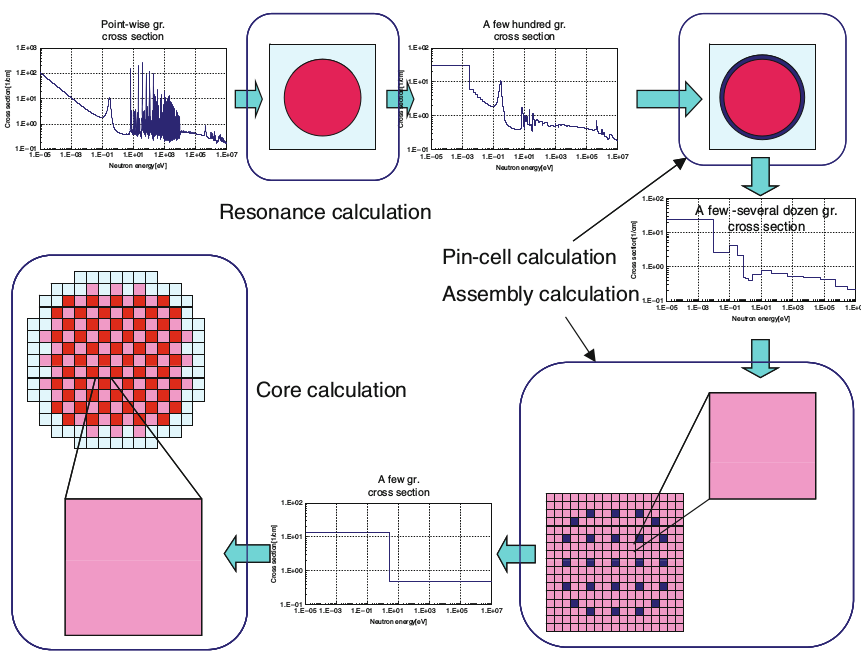
\includegraphics[width=0.9\linewidth]{figures/mgxs/nuke-handbook-mgxs-process}
\caption[]{}
\label{fig:chap2-mgxs-process}
\end{figure}

%\begin{dmath}
%\label{eqn:chap2-sigt-mg-color}
%\sigma_{t,n,i,g} = \frac{\int\displaylimits_{\mathbf{r} \in V_{i}} \int\displaylimits_{E_{g}}^{E_{g-1}} \sigma_{t,n}(\textcolor{carolinablue}{\mathbf{r}},\textcolor{darktangerine}{E})\phi(\textcolor{lightsalmonpink}{\mathbf{r}},\textcolor{lightgreen}{E})\mathrm{d}E\mathrm{d}\mathbf{r}}{\int\displaylimits_{\mathbf{r} \in V_{i}} \int\displaylimits_{E_{g}}^{E_{g-1}} \phi_{g}(\textcolor{lightsalmonpink}{\mathbf{r},\textcolor{lightgreen}{E}})\mathrm{d}E\mathrm{d}\mathbf{r}}
%\end{dmath}

\begin{figure}[h!]
  \centering
  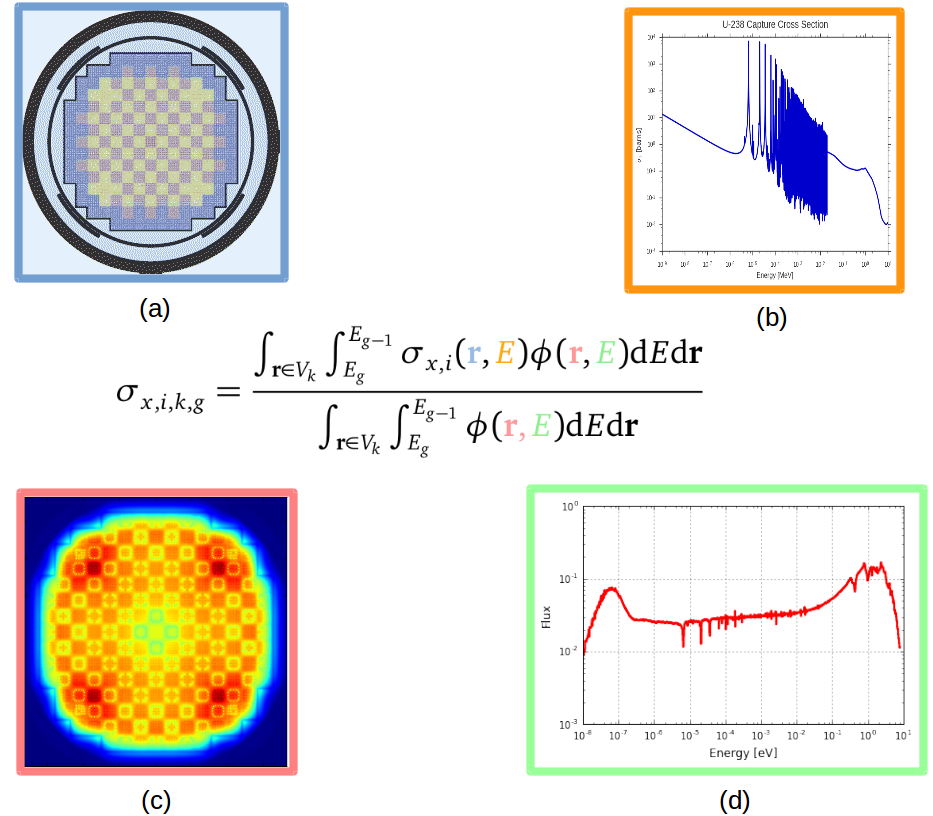
\includegraphics[width=0.9\linewidth]{figures/mgxs/mgxs-overlay}
\caption[]{}
\label{fig:chap2-mgxs-overlay}
\end{figure}


%%%%%%%%%%%%%%%%%%%%%%%%%%%%%%%%%%%%%%%%%%%%%%%%%%%%%%%%%%%%%%%%%%%%%%%%%%%%%%%
\section{MGXS Generation with Monte Carlo}
\label{sec:chap2-mgxs-mc}

\begin{itemize}[noitemsep]
  \item \ac{MC} is \emph{reactor agnostic}
  \item stochastic approx. to integrals in Section~\ref{sec:chap2-background}
\end{itemize}


%%%%%%%%%%%%%%%%%%%%%%
\subsection{Past Work}
\label{subsec:chap2-past-work}

\begin{itemize}[noitemsep]
  \item \ac{MGXS} for coarse mesh diffusion
  \begin{itemize}[noitemsep]
    \item Redmond
    \item Pounders
    \item Serpent
  \end{itemize}
  \item \ac{MGXS} for fine mesh transport
  \begin{itemize}[noitemsep]
    \item Nelson with NDPP
  \end{itemize}
\end{itemize}

%%%%%%%%%%%%%%%%%%%%%%%%%%%%%%%%%%%%%%%%%%%%%
\subsection{Spatial Self-Shielding Treatment}
\label{subsec:chap2-spatial-shield}

\begin{itemize}[noitemsep]
  \item spatial self-shielding treatment is natural in \ac{MC}
  \item challenge is slow convergence rate
  \item motivate clustering
\end{itemize}
\chapter{The Method of Characteristics}
\label{chap:moc}

In the previous chapter, some significant approximations are made in generation of multi-group cross-sections. Standard \ac{MOC} solvers, such as the one developed and discussed in this thesis, rely on multi-group cross-sections as input. Once the cross-sections are generated, \ac{MOC} is capable of computing reaction rates across the reactor geometry.

First, the \ac{MOC} equations are derived from the multi-group neutron transport equation. Then, track discretization is introduced, forming a system of equations involving discrete variables. Finally, the solution of the system of equations is discussed. Discussions of solution techniques to the \ac{MOC} system of equations normally are centered around the underlying physics with little mention of the system as a linear algebra problem~\cite{boyd2014openmoc}. Others further describe \ac{MOC} in terms of operator notation, but offer little insight into the structure of the operators~\cite{kochunas}. Instead, this discussion casts the system of equations as simply a general eigenvalue problem. Then discussion of matrix structure motivates the use of an uncommon solution technique. Physical reasoning for the structure is mentioned throughout the discussion. The properties of the chosen solution technique are discussed, motivating the need for an acceleration scheme to mitigate its weaknesses.


%%%%%%%%%%%%%%%%%%%%%%%%%%%%%%%%%%%%%%%%%%%%%%%%%%%%%%%%%%%%%%%%%%%%%%%%%%%%%%%
\section{Derivation of Continuous Angle MOC Equations}
\label{sec:derivation-of-moc}

Starting from the multi-group neutron transport equation given in Eq.~\ref{eqn:multi-group-transport}, the neutron source $q_g(\mathbf{r})$ is defined in Eq.~\ref{eqn:source},
\begin{equation}
q_g(\mathbf{r}) = \frac{1}{4 \pi} \left( \frac{\chi_{g}\left(\mathbf{r}\right)}{k} \sum_{g'=1}^{G} \nu_{g'}\left(\mathbf{r}\right) \Sigma_f^{g'}\left(\mathbf{r}\right) \phi_{g'}\left(\mathbf{r}\right) + \, \sum_{g'=1}^G \,  \Sigma_{s}^{g' \rightarrow g}\left(\mathbf{r}\right) \phi_{g'}(\mathbf{r}) \right)
\label{eqn:source}
\end{equation}
which leads to a new form for the neutron balance equation in Eq.~\ref{eqn:source-balance}.
\begin{dmath}
	\mathbf{\Omega} \cdot \nabla \psi_g(\mathbf{r},\mathbf{\Omega}) \, + \, \Sigma_{t}^{g}(\mathbf{r})\psi_g(\mathbf{r},\mathbf{\Omega}) = q_g(\mathbf{r})
	\label{eqn:source-balance}
\end{dmath}
Next, a coordinate transformation is performed, casting the position as a displacement from an origin $\mathbf{r_0}$ along the direction of travel $\mathbf{\Omega}$ as $\mathbf{r} = \mathbf{r_0} + s\mathbf{\Omega}$. Under this transformation, the new balance equation becomes:
\begin{dmath}
	\mathbf{\Omega} \cdot \nabla \psi_g(\mathbf{r_0} + s\mathbf{\Omega},\mathbf{\Omega}) \, + \, \Sigma_{t}^{i,g}(\mathbf{r_0} + s\mathbf{\Omega})\psi_g(\mathbf{r_0} + s\mathbf{\Omega},\mathbf{\Omega}) = q_g(\mathbf{r_0} + s\mathbf{\Omega})
\end{dmath}
In this new form, the gradient reduces to a simple derivative by the distance $s$ traveled from the origin $\mathbf{r_0}$ in Eq.~\ref{eqn:moc-transform}.
\begin{dmath}
	\frac{d\psi_g(\mathbf{r_0} + s\mathbf{\Omega},\mathbf{\Omega})}{ds} \, + \, \Sigma_{t}^{g}(\mathbf{r_0} + s\mathbf{\Omega})\psi(\mathbf{r_0} + s\mathbf{\Omega},\mathbf{\Omega}) = q_g(\mathbf{r_0} + s\mathbf{\Omega})
	\label{eqn:moc-transform}
\end{dmath}
Considering a region $i$ with constant total cross-section $\Sigma_{t}^{i,g}$, the angular flux a distance $\ell$ from the origin can be calculated using Eq.~\ref{eqn:moc-source-int}. The interested reader can find a simple derivation in Appendix~\ref{deriv:moc-source-int}.
\begin{dmath}
	\psi_g(\mathbf{r_0} + \ell \mathbf{\Omega},\mathbf{\Omega}) = \psi_g(\mathbf{r_0},\mathbf{\Omega}) e^{-\Sigma_{t}^{i,g} \ell} + \int\displaylimits_{0}^{\ell} ds \, e^{-\Sigma_{t}^{i,g} (\ell-s)}q_g(\mathbf{r_0} + s\mathbf{\Omega})
	\label{eqn:moc-source-int}
\end{dmath}

Eq.~\ref{eqn:moc-source-int} reveals an important relationship. For a region of constant total cross-section with known source distribution $q_g(\mathbf{r})$ and angular flux at a single point $\psi_g(\mathbf{r_0},\mathbf{\Omega})$, the angular flux for all points along the direction of travel $\mathbf{\Omega}$ can be calculated. Therefore an enclosing boundary defining the relationship of impinging angular fluxes is sufficient for the calculation of all angular fluxes within the region.

An example of one such boundary condition is the vacuum boundary condition where it is assumed that zero angular flux is impingent on the region for all angles. This is often used for full core problems since there are virtually no neutron sources outside the problem domain.

If the problem domain can be represented (or approximated) as the composition of a finite number of \textit{source regions} over which the total cross-section is constant and the neutron source $q_g(\mathbf{r})$ takes some known distribution, the calculation of all angular fluxes throughout the problem is straightforward.

Realistically, the source distribution is not known before solving the neutron transport equation, since it depends on the scalar fluxes. However, if the geometry is sufficiently discretized, a low order approximation of the \textit{shape} of the neutron source within the regions can be made with little impact on solution accuracy. An example of geometry discretization is shown in Fig.~\ref{fig:pin-discretization} where a fuel pin is discretized radially. The image on the left shows a radial view of the fuel pin geometry, colored by (constant cross-section) material region. The image on the right shows a discretized form of that geometry, colored by source region over which the neutron source is assumed to have some low-order form.

\begin{figure}[h!]
	\centering
	\begin{subfigure}{0.45\textwidth}
		\centering
		
\includegraphics[width=\linewidth]{figures/pin_1.PNG}
		\caption{}
		\label{fig:pin-discretization-a}
	\end{subfigure}
	\begin{subfigure}{0.45\textwidth}
		\centering
		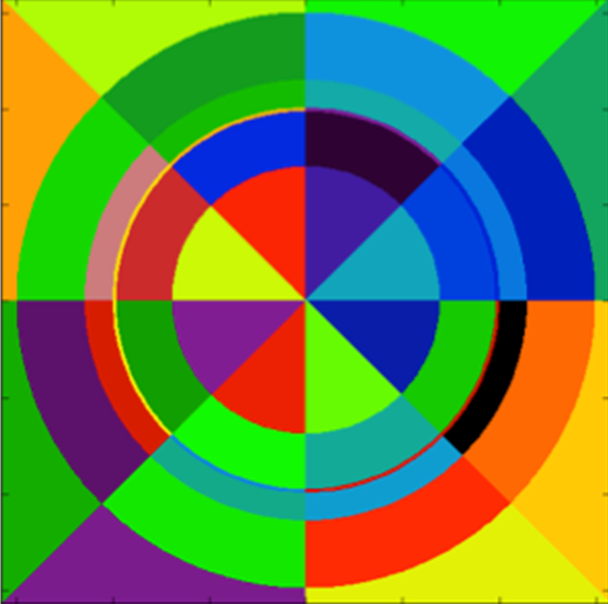
\includegraphics[width=\linewidth]{figures/pin_1_discretized.PNG}
		\caption{}
		\label{fig:pin-discretization-b}
	\end{subfigure}
	\caption[]{A description of source region discretization and mesh refinement. The geometry is shown (a) colored by material and (b) colored by source region.}
	\label{fig:pin-discretization}
\end{figure}

One common low order approximation for the neutron source is the flat source approximation. This approximation assumes the neutron source for a given energy group $q_g(\mathbf{r})$ is constant over each source region. A linear source approximation will be introduced later in Section~\ref{sec:linear-source}, allowing for a coarser discretization of the geometry. However, the flat source approximation is first presented in this description of \ac{MOC} as it is less mathematically cumbersome than the linear source approximation while arriving at a very similar form and solution method as the linear source version. The flat source approximation is also the most frequently used approximation in standard \ac{MOC} solvers~\cite{kochunas, FIXME}. Under this approximation the angular flux relationship given in Eq.~\ref{eqn:moc-source-int} reduces to
\begin{dmath}
	\psi_g(\mathbf{r_0} + \ell \mathbf{\Omega},\mathbf{\Omega}) = \psi_g(\mathbf{r_0},\mathbf{\Omega}) e^{-\Sigma_{t}^{i,g} \ell} + \int\displaylimits_{0}^{\ell} ds \, q^0_{i,g} e^{-\Sigma_{t}^{i,g} (\ell-s)}
\end{dmath}
with region $i$ having constant neutron source $q^0_{i,g}$. The integral can be analytically solved, leading to the final form given in Eq.~\ref{eqn:angular-flux-var}
\begin{dmath}
	\psi_g(\mathbf{r_0} + \ell \mathbf{\Omega},\mathbf{\Omega}) = \psi_g(\mathbf{r_0},\mathbf{\Omega}) e^{-\Sigma_{t}^{i,g} \ell} + \frac{q^0_{i,g}}{\Sigma_{t}^{i,g}} F_1 \left(\Sigma_{t}^{i,g} \ell\right)
	\label{eqn:angular-flux-var}
\end{dmath}
where
\begin{equation}
F_1(\tau) = 1 - e^{-\tau}.
\end{equation}

This equation allows for the computation of all necessary angular fluxes within a region of neutron source $q^0_{i,g}$. From the definition of the neutron source in Eq.~\ref{eqn:source}, the constant neutron source $q^0_{i,g}$ in the region $i$ can be computed as
\begin{equation}
q^0_{i,g} = \frac{1}{4 \pi} \left( \frac{\chi_{i,g}}{k} \sum_{g'=1}^{G} \nu_{i,g'} \Sigma_f^{i,g'} \overline{\phi_{i,g'}} + \, \sum_{g'=1}^G \,  \Sigma_{s}^{i,g' \rightarrow g} \overline{\phi_{i,g'}} \right)
\label{eqn:source-discr}
\end{equation}
where $\overline{\phi_{i,g}}$ is the average scalar flux in the region and the cross-sections have been taken to be constant over each region $i$. Recall from Eq.~\ref{eqn:scalar-flux} and integrating over region $i$ that the average scalar flux can be computed as:
\begin{dmath}
	\overline{\phi_{i,g}} = \frac{1}{V_i}\int_V dV \, \int_{4\pi} d\Omega \, \psi_g(\mathbf{r},\mathbf{\Omega})
	\label{eqn:avg-flux-theory}
\end{dmath}

This form is relatively unuseful since the relationship presented in Eq.~\ref{eqn:angular-flux-var} only applies for a specific direction. Therefore, the angular space is discretized into a finite number of directions. With the angular space discretized, the integral could be transformed into a weighted sum over the discrete directions, allowing the calculation of scalar fluxes.

\section{Track Discretization of the MOC Equations}

\ac{MOC} discretizes the angular space by choosing a finite number of directions to lay down \textit{tracks} across the geometry. For each direction, tracks stretch the entire length of the geometry, from one boundary to another, and completely fill the geometry. This collection of tracks is termed the \textit{track laydown}. A radial view of a coarse track laydown for a simple pin-cell geometry is shown in Figure~\ref{fig:track-laydown}. The geometry is colored by material region; namely water, clad, and fuel. Note that the final track laydown traverses tracks in both forward and backward directions rather than generating tracks in each direction for computational efficiency~\cite{kochunas2007twoway}.

%The left image shows the geometry, colored by material region; namely water, clad, and fuel. The middle image shows the track laydown across the geometry for one direction. The right image shows complete track laydown for four azimuthal directions.

\begin{figure}[h!]
	\centering
	\begin{subfigure}{0.3\textwidth}
		\centering
		
\includegraphics[width=\linewidth]{figures/pin_1.PNG}
		\caption{}
		\label{fig:track-laydown-a}
	\end{subfigure}
	\begin{subfigure}{0.3\textwidth}
		\centering
		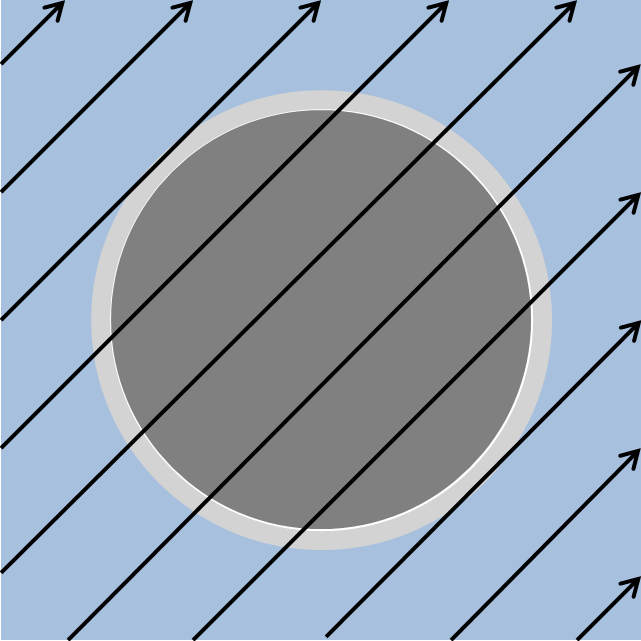
\includegraphics[width=\linewidth]{figures/pin_2.PNG}
		\caption{}
		\label{fig:track-laydown-b}
	\end{subfigure}
	\begin{subfigure}{0.3\textwidth}
		\centering
		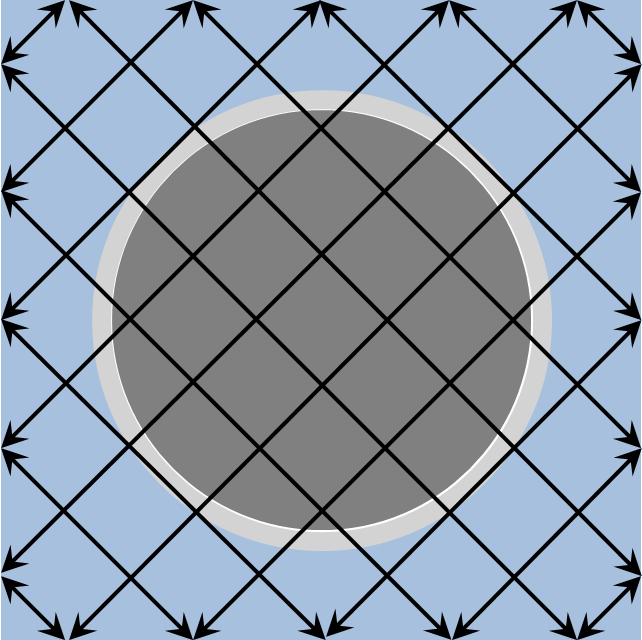
\includegraphics[width=\linewidth]{figures/pin_3.PNG}
		\caption{}
		\label{fig:track-laydown-c}
	\end{subfigure}
	\caption[]{A description of the track laydown process. The geometry (a) is shown followed by the track laydown (b) for one particular direction. Finally the entire track laydown for 4 azimuthal angles is shown (c) with arrows showing that each track is traversed both forward and backward. Note that the track laydowns shown here are significantly coarser than usual track laydowns for illustration purposes.}
	\label{fig:track-laydown}
\end{figure}

Across each track crossing a given constant cross-section source region, the variation of angular flux follows Eq.~\ref{eqn:angular-flux-var}. Therefore, each track is discretized into \textit{segments}, in which each segment is the portion of the track that crosses a particular source region. Across the entire length of each segment Eq.~\ref{eqn:angular-flux-var} applies. An illustration of the segmentation process for the simple pin-cell geometry is shown in Figure~\ref{fig:segmentation}. The presented track, with the geometry drawn along its direction of travel is discretized into segments by material region. For simplicity, this illustration does not discretize the geometry further than material boundaries. A real segmentation process would discretize segments over the domain shown in Figure~\ref{fig:pin-discretization-b}. This process would treat all tracks shown in the track laydown (eg. Figure~\ref{fig:track-laydown}) in a similar manner.

\begin{figure}[h!]
	\centering
	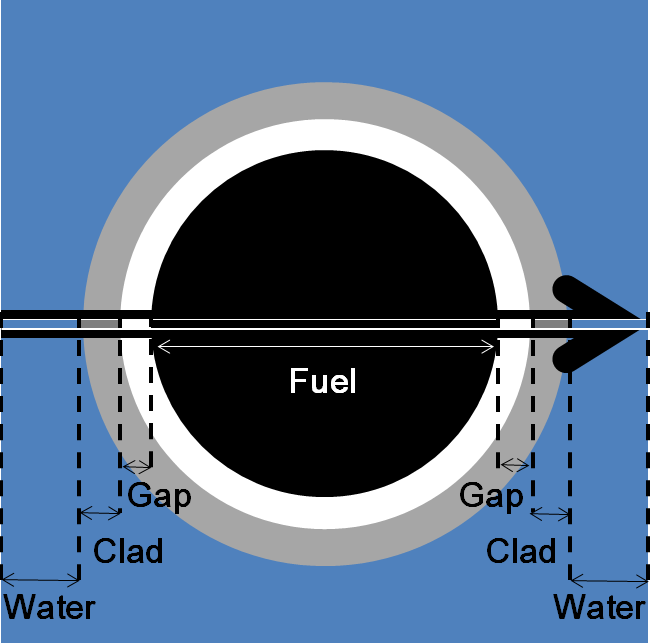
\includegraphics[width=0.6\linewidth]{figures/segmentation.PNG}
	\caption[]{The segmentation of a track horizontally traversing a pin-cell domain with coarse source discretization wherein the boundaries of source regions are no finer than their material region. The formed segments are colored by material region. For illustration purposes, the geometry is not shown to scale.}
	\label{fig:segmentation}
\end{figure}

All of these images showed track laydown and segmentation in just the radial plane, but the same methodology applies for dealing with full three dimensional geometries. Now that tracks have been segmented, a system of equations can be formed governing the variation of angular flux thorough each region as presented in Eq.~\ref{eqn:angular-flux-var}. However, this has a dependence on the incoming angular flux. For segments originating in the bulk of the geometry, continuity of angular flux is naturally enforced. The outgoing flux of the preceding segment in the track provides the incoming flux of the segment. Specifically, the position-dependent angular flux $\psi_{p,g}^{t,\varsigma}(\mathbf{r})$ in group $g$ along track $t$ and segment $\varsigma$ can be expressed as the angular flux of the preceding segment $\varsigma-1$ at the interface point $\mathbf{r_{\textbf{int}}}$ where the segments meet as
\begin{dmath}
	\psi_{p,g}^{t,\varsigma}(\mathbf{r_{\textbf{int}}}) = \psi_{p,g}^{t,\varsigma-1}(\mathbf{r_{\textbf{int}}}).
\end{dmath}
Defining the angular flux along a segment in terms of distance traveled along the segment rather than position, this can equivalently be written as
\begin{dmath}
	\psi_g^{t,\varsigma}(0) = \psi_g^{t,\varsigma-1}(\ell_{t,\varsigma-1})
	\label{eqn:angular_flux_boundary}
\end{dmath}
where $\ell_{t,\varsigma}$ refers to the length of segment $\varsigma$ along track $t$. For angular fluxes originating at the geometry boundary, the boundary condition provides the relationship for the angular flux. For vacuum boundary conditions, it is assumed that there is no impinging angular flux, so the incoming angular flux is simply taken to be zero at the boundary. 

For reflective boundary conditions, the incoming angular flux is equal to the outgoing angular flux of the reflected angle. This requires that a track be present with the correct reflecting angle, meeting at precisely the same point on the boundary. During track laydown, this is enforced. If only vacuum boundary conditions were present, this restriction on track laydown would not be necessary. Similar treatments are possible for periodic and rotational boundary conditions if allowed by the track laydown.  A more complete discussion of track laydown is given in Chapter~\ref{chap:track-laydown}. For instance, the conditions required to link tracks at geometric boundaries will be discussed at length.

Precise definitions are needed in order to discuss the relation of these tracks to the \ac{MOC} equations. Tracks are defined to originate at one boundary and stretch across the geometry until they terminate at another boundary. The segments of a track are ordered in the direction of the track so that only the first segment is affected by a boundary condition. Track $t$ is defined to have $S(t)$ segments. For vacuum boundaries,
\begin{dmath}
	\psi_g^{t,1}(0) = 0
\end{dmath}
For boundary conditions (such as reflective, periodic, and rotational) that connect with another track, the function $C$ is defined which defines the linking track. For instance, the incoming angular flux of track $t$ would connect with the outgoing angular flux of track $C(t)$ as
\begin{dmath}
	\psi_g^{t,1}(0) = \psi_g^{C(t),S(C(t))}(\ell_{C(t),S(C(t))})
	\label{eqn:linking-bc}
\end{dmath}

With the angular and spatial discretization from the track laydown, the angular flux relationship along a characteristic path given in Eq.~\ref{eqn:angular-flux-var} can be presented in terms of the discretized track segments in Eq.~\ref{eqn:angular-flux-var-disc} where the function $R$ yields the region traversed by track $t$ and segment $\varsigma$. 
\begin{dmath}
	\psi_g^{t,\varsigma}(s) = \psi^{t,\varsigma}_g(0) + \left( \frac{q^0_{R(t,\varsigma),g}}{\Sigma_{t}^{i,g}} - \psi_g^{t,\varsigma}(0) \right) F_1\left(\Sigma_{t}^{R(t,\varsigma),g} s \right)
	\label{eqn:angular-flux-var-disc}
\end{dmath}
Still, these equations only determine the behavior of the neutron flux along a particular track. To determine the behavior of the neutron flux throughout the geometry, an infinite number of tracks would be required so that every point in the geometry lies along one of the tracks. Therefore, an approximation is invoked in which all points within the geometry are characterized by the nearest track. Therefore each track represents a volume formed by the product of its length and the perpendicular distances to tracks of the same direction. Those perpendicular lengths form the track cross-sectional area as illustrated in Figure~\ref{fig:track-cross-section}. This illustration just shows the radial view of the tracks. However, in three dimensions, axial distances also exist between tracks so that the track cross-sectional area does indeed represent an area rather than a distance.
\begin{figure}[h!]
	\centering
	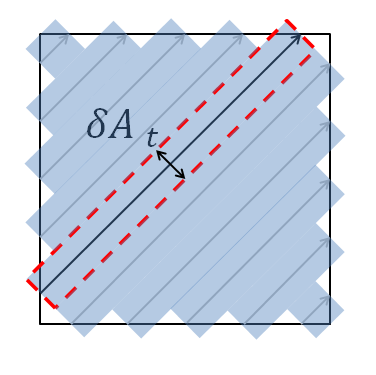
\includegraphics[width=0.6\linewidth]{figures/track-cross-sectional-area.PNG}
	\caption[]{An illustration of the spatial volume represented by each track as the product of track length and track cross-sectional area $\delta A_t$. The volume represented by each track is shaded in blue.}
	\label{fig:track-cross-section}
\end{figure}
With a fine track laydown where the distance between tracks becomes small, the approximation error of assuming points within the geometry are characterized by the nearest track also becomes small. 

However, the neutron transport equation has an angular dependence in addition to a spatial dependence. Therefore, fully resolving the angular dependence would require a track at every direction, again leading to an infinite number of tracks. Similar to the approximation invoked to cover the entire geometric space, the behavior of the neutron flux at each direction is characterized by the track with the most similar direction. This leads to each track $t$ having an angular weight $\alpha_t$ relating to the width of the angular space represented by the track. Therefore the overall weight of the track $w_t$ is calculated as the product of track cross-sectional area and angular weight as given in Eq.~\ref{eqn:weight-def}.
\begin{equation}
w_{t} = \delta A_{t} \alpha_t
\label{eqn:weight-def}
\end{equation}
With each track now representing a portion of the spatial and angular domain, Eq.~\ref{eqn:avg-flux-theory} can be transformed to reflect the track discretization in Eq.~\ref{eqn:average-flux-disc}, yielding a closed-form relationship to calculate the scalar flux.
\begin{dmath}
	\overline{\phi_{i,g}} = \frac{1}{V_i} \sum_{(t,\varsigma) \in V_i} w_{t} \int_{0}^{\ell_{t,\varsigma}} ds \, \psi^{t,\varsigma}_g(s)
	\label{eqn:average-flux-disc}
\end{dmath}
Combining Eq.~\ref{eqn:average-flux-disc} with Eq.~\ref{eqn:angular-flux-var-disc}, the scalar flux can be calculated using the relationship in Eq.~\ref{eqn:average-flux}. A proof is given in Appendix~\ref{deriv:avg-flux} for the interested reader.
\begin{dmath}
	\overline{\phi_{i,g}} = \frac{q^0_{i,g}}{\Sigma_{t}^{i,g}} + \frac{1}{\Sigma_{t}^{i,g} V_i} \sum_{(t,\varsigma) \in V_i} w_{t} \Delta \psi_g^{t,\varsigma}
	\label{eqn:average-flux}
\end{dmath}
The difference in angular flux $\Delta \psi_g^{t,\varsigma}$ is equal to $\psi_g^{t,\varsigma}(0) - \psi_g^{t,\varsigma}(\ell_{t,\varsigma})$. The calculated fluxes can then be used to construct the neutron sources $q^0_{i,g}$ for each region $i$ and each energy group $g$ with the relationship in Eq.~\ref{eqn:source-discr}.


\section{Solving the MOC System of Equations}
\label{sec:moc-solve}

In the previous section Eq.~\ref{eqn:angular-flux-var-disc} and Eq.~\ref{eqn:average-flux} provided ways to calculate the angular fluxes and scalar fluxes, respectively. The source can be computed from the scalar fluxes with Eq.~\ref{eqn:source-discr}. This forms a system of equations that can be solved to determine the neutron distribution inside a nuclear reactor core. Normally, the solution of the \ac{MOC} equations is presented in terms of a physics perspective, following neutrons along trajectories, and repeatedly solving for the neutron source. Physical intuition usually guides this discussion.

The discussion presented here will be more broad. Instead of solely focusing on physics, the problem will be cast as a set of matrix equations that could theoretically be solved with common linear algebra packages. However, this discussion will show that blindly solving the system of equations with a general linear algebra package is computationally infeasible since it loses sight of inherent structure the physics-based approach naturally captures.

The system of equations to be solved is formed by Eq.~\ref{eqn:source-discr}, Eq.~\ref{eqn:angular-flux-var-disc}, and Eq.~\ref{eqn:average-flux}. Turning Eq.~\ref{eqn:source-discr} into matrix form, a fission matrix $F$ and a scattering matrix $S$ are defined such that
\begin{equation}
\mathbf{q} = \frac{1}{k} F \boldsymbol{\phi} + S \boldsymbol{\phi}
\label{eqn:matrix-source-calc}
\end{equation}
where $\mathbf{q}$ is a vector of size $M$ containing all neutron sources and $\boldsymbol{\phi}$ is a vector of size $M$ containing all scalar fluxes. Since there must be a neutron source and scalar flux for every source region and every energy group, $M = L G$ where $L$ is the number of source regions and $G$ is the number of groups. The scalar fluxes $\boldsymbol{\phi}$ as well as the sources $\mathbf{q}$ are ordered such that they are contiguous in group with the index calculated as $i G + g$. In the context of this discussion, elements relating to region quantities are indexed by source region $i$ and group $g$, yielding the following definitions for the fission matrix $F$ and scattering matrix $S$ as
\begin{eqnarray}
F_{\left(i, g\right), \, \left(i, g'\right)} = \frac{1}{4\pi} \chi_{i,g} \nu \Sigma_f^{i,g'}
\label{eqn:fission-matrix}
\end{eqnarray}
and
\begin{eqnarray}
S_{\left(i, g\right), \, \left(i, g'\right)} = \frac{1}{4\pi} \Sigma_s^{i,g' \rightarrow g}
\label{eqn:scattering-matrix}
\end{eqnarray}
where all other unspecified matrix elements are zero. Both of these matrices are of size $M \times M$ and sparse since there are no inter-regional terms.

The relationship in Eq.~\ref{eqn:angular-flux-var-disc} can be rearranged to form the relationship in Eq.~\ref{eqn:re-angular-flux-var-disc}. This form is much easier to work with in the translation to matrix definitions.
\begin{equation}
 \psi^{t,\varsigma}_g(0) \left(\frac{F_1\left(\Sigma_{t}^{i,g} s \right) - 1}{F_1\left(\Sigma_{t}^{i,g} s \right)}\right) + \psi_g^{t,\varsigma}(s) \left(\frac{1}{F_1\left(\Sigma_{t}^{i,g} s \right)}\right) = \frac{q^0_{i,g}}{\Sigma_{t}^{i,g}}
\label{eqn:re-angular-flux-var-disc}
\end{equation}
This relationship can be turned into matrix form by defining an angular flux vector $\boldsymbol{\psi}$ that contains all outgoing angular fluxes. This is represented in Eq.~\ref{eqn:matrix-attn} by an angular flux transport matrix $T$ defining relationships between angular fluxes, a source selection matrix $H$ which selects the source of the region being traversed, and a diagonal matrix $D$ containing the total cross-sections which scale the source appropriately to match the relationship in Eq.~\ref{eqn:re-angular-flux-var-disc}.
\begin{equation}
T \boldsymbol{\psi} = H D^{-1} \mathbf{q}
\label{eqn:matrix-attn}
\end{equation}
The number of angular fluxes is $N = \beta L G$ where $\beta$ is the average number of track crossings per source region. Since there must be a significant number of track crossings per region for convergence we expect $N >> M$. $T$ is size $N \times N$ as it defines relationships between angular fluxes, the size of $H$ is $N \times M$ since for each angular flux pair it must pick out the appropriate source region, and the size of $D$ is $M \times M$ since it relates only to the source regions. The elements relating to angular flux quantities are indexed by track $t$, segment $\varsigma$, and group $g$. The source selection matrix $H$ can therefore be defined as
\begin{equation}
H_{\left(t,\varsigma,g\right), \, \left(R(t,\varsigma), g\right)} = 1.
\label{eqn:source-selection-matrix}
\end{equation}
This matrix therefore, has only one non-zero value per row, indicating which region is being traversed, relating track-based quantities such as angular fluxes to region based quantities such as the scalar fluxes. Its transpose similarly relates the regions to the tracks traversing the region. The matrix $H^T H$ is a $M \times M$ diagonal matrix with each diagonal element representing the number of tracks that traverse the region multiplied by the number of groups. Since it is diagonal, it is easily invertible, which will be important in the later discussion.
The diagonal matrix $D$ containing the total cross-sections is defined by
\begin{equation}
D_{\left(i, g\right), \, \left(i, g\right)} = \Sigma_t^{i,g}.
\label{eqn:total-xs-matrix}
\end{equation}
The angular flux transport matrix $T$ is defined by
\begin{equation}
T_{\left(t,\varsigma,g\right), \, \left(t, \varsigma, g\right)} = \frac{1}{F_1\left(\Sigma_{t}^{R(t,\varsigma),g} \ell_{t,\varsigma}\right)}
\label{eqn:angular-flux-transport-matrix-1}
\end{equation}
and
\begin{equation}
T_{\left(t,\varsigma,g\right), \, \left(t, \varsigma-1, g\right)} = \frac{F_1\left(\Sigma_{t}^{R(t,\varsigma),g} \ell_{t,\varsigma}\right) - 1}{F_1\left(\Sigma_{t}^{R(t,\varsigma),g} \ell_{t,\varsigma}\right)}.
\label{eqn:angular-flux-transport-matrix-2}
\end{equation}
Again, all non-specified quantities are zero.

Lastly, Eq.~\ref{eqn:average-flux} describes how the scalar flux can is calculated in terms of both a weighted sum of angular fluxes and the neutron source. Specifically, an angular flux weighting matrix $W$ of size $M \times N$ is defined such that
\begin{equation}
\boldsymbol{\phi} = D^{-1}\mathbf{q} + D^{-1} W \boldsymbol{\psi}.
\label{eqn:matrix-flux-calc}
\end{equation}
In order to expose its structure, $W$ is expressed as a multiplication of matrices
\begin{equation}
W = V^{-1} H^T \tilde{W}
\end{equation}
where the volume matrix $V$ is a $M \times M$ diagonal matrix containing region volumes as
\begin{equation}
V_{\left(i, g\right), \, \left(i, g\right)} = V_i
\end{equation}
and $\tilde{W}$ is an $N \times N$ matrix defined by
\begin{equation}
\tilde{W}_{\left(t,\varsigma,g\right), \, \left(t, \varsigma, g\right)} = -w_{t}
\end{equation}
and
\begin{equation}
\tilde{W}_{\left(t,\varsigma,g\right), \, \left(t, \varsigma-1, g\right)} = w_{t}
\end{equation}
with all other elements being zero. Now that all matrix elements have been defined, the transport equation can be written as a matrix eigenvalue problem. Combining Eq.~\ref{eqn:matrix-source-calc} and Eq.~\ref{eqn:matrix-flux-calc} yields
\begin{equation}
\boldsymbol{\phi} = D^{-1} \left(\frac{1}{k} F + S \right) \boldsymbol{\phi} + D^{-1} W \boldsymbol{\psi}
\end{equation}
which combined with Eq.~\ref{eqn:matrix-attn} yields
\begin{equation}
\boldsymbol{\phi} = D^{-1}\left( I + W T^{-1} H D^{-1}\right) \left(\frac{1}{k} F + S \right) \boldsymbol{\phi}
\label{eqn:moc-matrix-form}
\end{equation}
where $I$ is the identity matrix of dimension $M \times M$. This relationship can be further simplified by defining a matrix $J$ such that
\begin{equation}
J = D^{-1}\left( I + W T^{-1} H D^{-1}\right)
\end{equation}
leading to the expression
\begin{equation}
\boldsymbol{\phi} = J \left(\frac{1}{k} F + S \right) \boldsymbol{\phi}
\label{eq:transport-simplified}
\end{equation}
This results in the generalized eigenvalue equation given in Eq.~\ref{eqn:gen-eig}
\begin{equation}
A \boldsymbol{\phi} = k B \boldsymbol{\phi}
\label{eqn:gen-eig}
\end{equation}
where
\begin{equation}
A = JF
\end{equation}
and
\begin{equation}
B = I - JS.
\end{equation}
This can of course be turned into a regular eigenvalue problem by explicitly taking the inverse as
\begin{equation}
B^{-1}A \boldsymbol{\phi} = k \boldsymbol{\phi}.
\label{eqn:eig}
\end{equation}
At this point, the matrix $B^{-1}A$ could be explicitly calculated and then input into any standard eigenvalue solver. However, taking matrix inverses is very computationally intense, especially due to the internal structure of $A$ and $B$. Specifically, since $J$ involves the inverse of $T$, even the explicit computation of its elements is infeasible. Therefore, doing this would be very unwise. Even if a generalized eigenvalue solver is available capable of solving equations of the form given in Eq.~\ref{eqn:gen-eig}, the problem would still rely on computing explicit components of $J$. Even though the steady-state neutron transport equation is an eigenvalue problem defined in terms of the angular fluxes, they only enter the equation implicitly with the inversion of $T$. 

%Moreover, the reaction rates of interest are defined in terms of the scalar fluxes. From angular fluxes, it is simple to calculate the scalar fluxes. This structure is an indication that explicitly solving for the full vector of angular fluxes is unnecessary.

Therefore, instead of using a common eigenvalue solution technique, a variation of fixed point iteration termed \textit{source iteration} is chosen to solve the system. In this procedure, the relationship in Eq.~\ref{eqn:moc-matrix-form} is used with the right hand side of the equation lagged as
\begin{equation}
\boldsymbol{\phi}_{n+1} = D^{-1}\left( I + W T^{-1} H D^{-1}\right) \left(\frac{1}{k_n} F + S \right) \boldsymbol{\phi}_n
\end{equation}
where the subscript $n$ indicates iteration number. Mechanically, the process iterates over estimations of the neutron source, calculating the corresponding fluxes. First, an initial flux distribution is guessed along with a value for the eigenvalue $k$. At the start of each iteration, the source distribution $\mathbf{q}$ is calculated using Eq.~\ref{eqn:matrix-source-calc} from the current guess of scalar fluxes $\boldsymbol{\phi}$ and eigenvalue $k$. Then, during the \textit{transport sweep}, new angular fluxes are computed as
\begin{equation}
\boldsymbol{\psi} = T^{-1} H D^{-1} \mathbf{q}.
\end{equation}
First, the computation of $HD^{-1}\mathbf{q}$ is trivial since $H$ is just the source selection matrix and $D$ is diagonal. Physically, this just relates to picking out the source region being traversed and calculating the source divided by the total cross-section.

Due to the simple structure of $T$, solving its implicit inversion is rather simple. $T$ has just one element on the diagonal and one off-diagonal element per row. Note that the angular fluxes are only related to their associated connecting angular flux. For some boundary conditions (e.g. reflective), the connecting angular flux might be from another track. This could cause the inversion to be somewhat difficult. If all boundaries have this characteristic, all the angular fluxes within a cycle of connecting tracks would be dependent on each other.

To alleviate this issue, the angular fluxes at boundaries are approximated by the calculated angular flux at the boundary from the previous iteration. Specifically, the relationship in Eq.~\ref{eqn:angular_flux_boundary} relating connecting angular fluxes at the start of a track is approximated by
\begin{dmath}
	\psi_g^{t,1}(0) = \widetilde{\psi}_g^{C(t),S(C(t))}(\ell_{C(t),S(C(t))})
\end{dmath}
where $\widetilde{\psi}$ represents the calculated angular fluxes from the previous iteration so that $\widetilde{\psi}_g^{C(t),S(C(t))}$ is the angular flux of the connecting track from the previous iteration. This transformation allows the inversion of $T$ to be calculated using an altered matrix $\tilde{T}$ which lacks dependency between different tracks, then adding the contribution of the previous iteration angular fluxes, if applicable. The structure of $\tilde{T}$ is block-diagonal and within each block the matrix is upper triangular. Physically this means that all tracks can be calculated independently of each other during an iteration. For each track, the angular fluxes can be solved sequentially by segment. This is where the \textit{transport sweep} owes its name as the algorithm simply sweeps over segments. Since each row has at most two elements, very little calculation is required for each angular flux. 

During this process, it is noted that only the boundary angular fluxes along with the neutron source are needed to determine all angular fluxes. Therefore, non-boundary angular fluxes are computed on-the-fly. Furthermore, the elements of $T$ are re-computed on-the-fly. Since the computation of the scalar fluxes $\boldsymbol{\phi}$ relies on a weighted sum of the full angular flux vector $\boldsymbol{\psi}$, once an angular flux is computed its contribution to the scalar fluxes is tallied before it is discarded.

After the transport sweep, the source is added to the scalar flux tally, consistent with Eq.~\ref{eqn:matrix-flux-calc}, to produce a new estimate of the scalar fluxes $\boldsymbol{\phi}$. To form a new estimate of $k$, note that
\begin{equation}
T \boldsymbol{\psi} = \frac{1}{k} H D^{-1} F \boldsymbol{\phi} + H D^{-1} S \boldsymbol{\phi}
\end{equation}
which then is re-arranged and multiplied with a vector of ones $\mathbb{1}_M$ of length $M$ as
\begin{equation}
\mathbb{1}_M^T D H_{\text{left}}^{-1} T \boldsymbol{\psi}  = \frac{1}{k} \mathbb{1}_M^T  F \boldsymbol{\phi} + \mathbb{1}_M^T  S \boldsymbol{\phi}.
\end{equation}
Since $H$ is rectangular, it cannot be simply inverted. But since it is of full rank, $H^T H$ can be inverted. From the previous discussion of $H$, recall that $H^T H$ is diagonal so its inversion is simple. Therefore the left inverse $H_{\text{left}}^{-1}$ of matrix $H$ is defined to be
\begin{equation}
H_{\text{left}}^{-1} = \left(H^T H\right)^{-1} H^T.
\end{equation}
This allows the eigenvalue $k$ to be computed as
\begin{equation}
k = \frac{\mathbb{1}_M^T F \boldsymbol{\phi}}{\mathbb{1}_M^T  D H_{\text{left}}^{-1} T \boldsymbol{\psi} - \mathbb{1}_M^T S \boldsymbol{\phi}}.
\end{equation}
Combining Eq.~\ref{eqn:matrix-attn} and Eq.~\ref{eqn:matrix-flux-calc}, note that
\begin{equation}
D H_{\text{left}}^{-1} T \boldsymbol{\psi} = D \boldsymbol{\phi} - W \boldsymbol{\psi}
\end{equation}
and therefore
\begin{equation}
k = \frac{\mathbb{1}_M^T F \boldsymbol{\phi}}{\mathbb{1}_M^T \left(D - S \right) \boldsymbol{\phi} - \mathbb{1}_M^T W \boldsymbol{\psi}}.
\end{equation}
where $\mathbb{1}_M^T F \boldsymbol{\phi}$ refers to the fission rate, $\mathbb{1}_M^T \left(D - S \right) \boldsymbol{\phi}$ refers to the absorption rate, and $-\mathbb{1}_M^T W \boldsymbol{\psi}$ refers to the leakage rate. Physically, this shows that $k$ is simply a ratio of neutron production to neutron loss terms.

Notice that each source iteration relies on simply taking the inverse of the transport matrix $T$ rather than the full $B$ matrix, which includes the scattering matrix, as would normally be taken during an eigenvalue solver, e.g. power iteration. While this choice does ease the computational burden of each iteration, it also requires many more iterations to converge to the correct solution as each iteration does little work in resolving the angular fluxes as the scattering matrix is not included in the inversion. Physically, this relates to not treating the scattering source as directly coupled to the total neutron source. Therefore, un-accelerated \ac{MOC} is inherently plagued by slow convergence. 

Next, in Chapter~\ref{chap:cmfd}, Course Mesh Finite Difference (CMFD) acceleration is introduced which resolves the issue of slow convergence for source iteration. This allows for the computational burden of each iteration to be eased without giving up anything in terms of convergence rate by iteration.

\newpage
\vfill
\begin{highlightsbox}[frametitle=Highlights]
	\begin{itemize}
		\item The \ac{MOC} transform changes the neutron transport equation from a partial differential equation to an ordinary differential equation along a certain direction.
		\item The geometry is discretized into source regions which have constant cross-sections and a low-order approximation of the neutron source within the region.
		\item Tracks are laid down across the geometry which enable the  \ac{MOC} transform to yield an analytic description of the angular flux variation across each source region.
		\item The angular flux variation along each track provided a weighted contribution to the scalar flux estimate of each traversed source region.
		\item The synthesis of \ac{MOC} equations over each source region form an eigenvalue problem.
		\item The \ac{MOC} eigenvalue problem fundamentally involves all angular fluxes over each source region.
		\item Since the number of angular fluxes is vast, standard eigenvalue solution techniques are abandoned in favor of \textit{source iteration} which takes advantage of fundamental structure of the \ac{MOC} equations.
		\item \textit{Source iteration} allows each \ac{MOC} iteration to be computed far more efficiently in the form of a \textit{transport sweep} but at the cost of slow convergence (if acceleration is absent)
	\end{itemize}
\end{highlightsbox}


%\begin{equation}
%\left(I - JS\right)^{-1} JF \boldsymbol{\phi} = k \boldsymbol{\phi}
%\end{equation}

%\begin{equation}
%A \boldsymbol{\phi} = k \boldsymbol{\phi}
%\end{equation}

%\begin{equation}
%\boldsymbol{\phi}_{n+1} = J \left(\frac{1}{k_n} F + S\right) \boldsymbol{\phi}_n
%\end{equation}

%\begin{equation}
%\boldsymbol{\phi}_{n+1} = J \left(\frac{1}{k} F + S\right) \boldsymbol{\phi}_n
%\end{equation}

%\begin{equation}
%\boldsymbol{\phi}_{n+1} = B \boldsymbol{\phi}_n
%\end{equation}

%\begin{equation}
%B \boldsymbol{\phi} = \lambda \boldsymbol{\phi}
%\end{equation}


%\begin{equation}
%\boldsymbol{\phi} + C \boldsymbol{\phi} = J \left(\frac{1}{k} F + S\right) \boldsymbol{\phi} + C \boldsymbol{\phi}
%\end{equation}

%\begin{equation}
%\left(I + C\right)\boldsymbol{\phi}_{n+1} = J \left(\frac{1}{k_n} F + S\right) \boldsymbol{\phi}_n + C \boldsymbol{\phi}_n
%\end{equation}

%\begin{equation}
%\boldsymbol{\phi}_{n+1} = \left(I + C\right)^{-1} \left[J \left(\frac{1}{k_n} F + S\right) + C\right] \boldsymbol{\phi}_n
%\end{equation}
\chapter{CMFD Acceleration}
\label{chap:cmfd}

In the previous section, the poor convergence of source iteration to solve the MOC equations was discussed. In this section, Course Mesh Finite Difference (CMFD) acceleration is introduced which allows for better convergence. During CMFD acceleration, a course mesh problem is solved that is consistent with the fine mesh MOC problem. Since the course mesh problem can be solved quickly, it can be fully converged and used to update the MOC solution allowing global behavior to be communicated in fewer iterations. This section discuss CMFD as a multigrid method, shows how the CMFD equations are derived from the fundamental multi-group transport equation, and then the process of applying CMFD acceleration is discussed.

%%%%%%%%%%%%%%%%%%%%%%%%%%%%%%%%%%%%%%%%%%%%%%%%%%%%%%%%%%%%%%%%%%%%%%%%%%%%%%%
\section{Multigrid Methods}
\label{sec:multigrid}

Multigrid methods are popular in numerical analysis for solving differential equations. The fundamental idea is that global information can be transferred much quicker over a coarse mesh that a fine mesh. Using this principle multigrid methods alternate between solving the set of equations on a coarse mesh, where the problem size is reduced and information propagates much quicker, and a fine mesh where the discretization accurately captures the solution of the problem. It is vital that the coarse mesh solution be consistent with the fine mesh solution. In this context, consistency means that at convergence the coarse mesh and fine mesh solutions agree.

Multigrid methods can be structured in many different ways but they generally involve two important stages: restriction and prolongation.
\begin{itemize}
	\item \textbf{Restriction - } Collapsing the fine mesh solution down to a consistent form on a coarse mesh.
	\item \textbf{Prolongation - } Using the coarse mesh solution to interpolate corrections to the fine mesh solution.
\end{itemize}

Multigrid methods in general can involve many layers of mesh. At each layer, restriction and prolongation are used to transfer to coarser and finer mesh layers, respectively. However, for the CMFD acceleration scheme implemented in this thesis, only two layers of mesh are used: the fine MOC mesh and the coarse CMFD mesh. Figure~\ref{fig:multigrid-cmfd} illustrates the process of solving the MOC equations using CMFD acceleration.
\begin{figure}[h!] 
	\centering 
	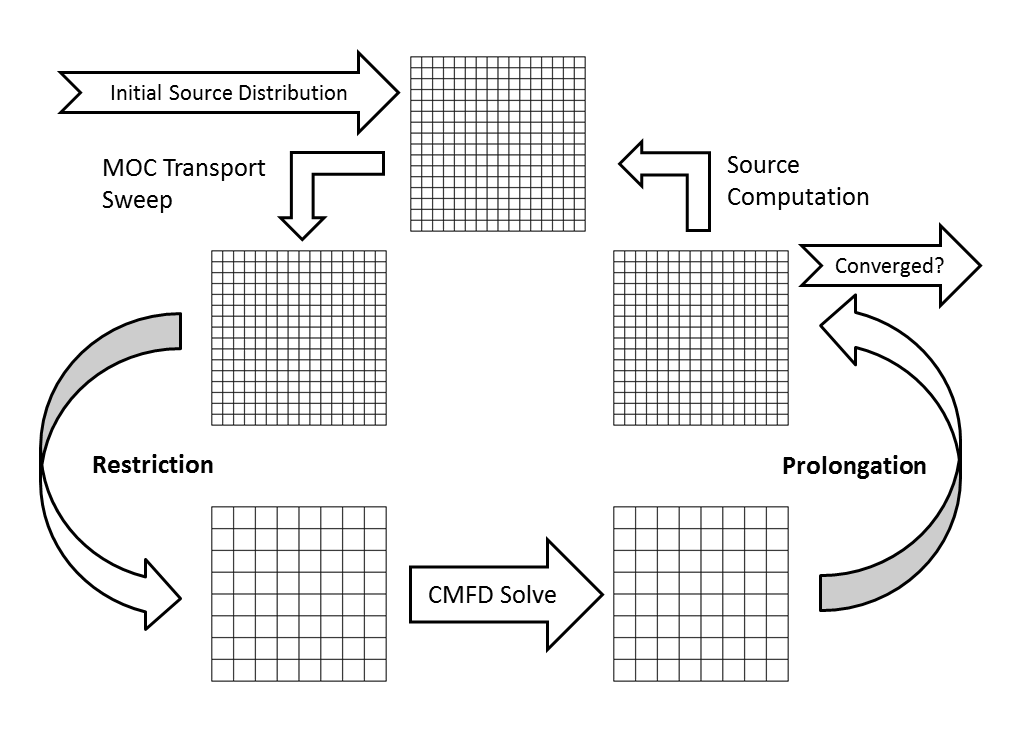
\includegraphics[width=\linewidth]{figures/multigrid-cmfd.PNG}
	\caption[]{A depiction of the multigrid approach to solving the MOC transport equations with CMFD acceleration.}
	\label{fig:multigrid-cmfd}
\end{figure}

One important difference between usual multigrid approaches and CMFD is that the CMFD equations are solved using consistent but fundamentally different equations. Instead of solving the coarse mesh problem using the same MOC form of the neutron transport equation, where the angular space is discretized using tracks, the CMFD equations rely on diffusion theory. This alternate form of the transport equation relies strictly on cell averaged quantities rather than having a dependence on angular directions. To enforce consistency with the MOC solution, surface currents are tallied during the MOC solve. Section~\ref{sec:cmfd-derivation} details the derivation of the diffusion form of the neutron transport equation with term definitions from the MOC equations for consistency.

%%%%%%%%%%%%%%%%%%%%%%%%%%%%%%%%%%%%%%%%%%%%%%%%%%%%%%%%%%%%%%%%%%%%%%%%%%%%%%%
\section{Derivation of the CMFD Equations}
\label{sec:cmfd-derivation}

The CMFD equations can be derived from the fundamentals of multi-group transport. The general concept is to turn the transport equation, which is fundamentally based on angular fluxes into a diffusion problem which is fundamentally based on scalar fluxes averaged over some volume in the reactor. During this process, some approximations will be introduced. However, all of these approximations introduce no bias at convergence. Therefore they do not impact solution accuracy. First recall the multigroup approximation given in Eq.~\ref{eqn:multi-group-transport}:
\begin{equation}
	\mathbf{\Omega} \cdot \nabla \psi_{g}(\mathbf{r},\mathbf{\Omega}) + \Sigma_t^{g}(\mathbf{r}) \psi_{g}(\mathbf{r},\mathbf{\Omega}) = \frac{1}{4 \pi} \left( \frac{\chi_{g}\left(\mathbf{r}\right)}{k} \sum_{g'=1}^{G} \nu_{g'}\left(\mathbf{r}\right) \Sigma_f^{g'}\left(\mathbf{r}\right) \phi_{g'}\left(\mathbf{r}\right) + \, \sum_{g'=1}^G \,  \Sigma_{s}^{g' \rightarrow g}\left(\mathbf{r}\right) \phi_{g'}(\mathbf{r}) \right)
\end{equation}
To transform this equation into one based on the scalar fluxes $\phi_{g}(\mathbf{r})$ rather than the angular fluxes $\psi_{g}(\mathbf{r},\mathbf{\Omega})$, the equation is integrated over the entire $4\pi$ angular space. In doing so, recall from Eq.~\ref{eqn:scalar-flux} that the integral of angular flux over the entire angular space is simply the scalar flux, leading to the relationship in Eq.~\ref{eqn:angle_int_transport}.
\begin{equation}
	\int\displaylimits_{4 \pi} d\mathbf{\Omega} \,\mathbf{\Omega} \cdot \nabla \psi_{g}(\mathbf{r},\mathbf{\Omega}) + \Sigma_t^{g}\left(\mathbf{r}\right) \phi_{g}(\mathbf{r}) = \frac{\chi_{g}\left(\mathbf{r}\right)}{k} \sum_{g'=1}^{G} \nu_{g'}\left(\mathbf{r}\right) \Sigma_f^{g'}\left(\mathbf{r}\right) \phi_{g'}(\mathbf{r}) + \, \sum_{g'=1}^G \,  \Sigma_{s}^{g' \rightarrow g}\left(\mathbf{r}\right) \phi_{g'}(\mathbf{r})
	\label{eqn:angle_int_transport}
\end{equation}
Notice that only the streaming term has any dependence on the angular flux $\psi_{g}(\mathbf{r},\mathbf{\Omega})$. Since the angular variable $\mathbf{\Omega}$ is independent of the spatial variable $\mathbf{r}$, the gradient can be brought outside the integral in the streaming term as shown in Eq.~\ref{eqn:angle_int_transport_grad}.
\begin{equation}
	\nabla \cdot \int\displaylimits_{4 \pi} d\mathbf{\Omega} \,\mathbf{\Omega} \psi_{g}(\mathbf{r},\mathbf{\Omega}) + \Sigma_t^{g}\left(\mathbf{r}\right) \phi_{g}(\mathbf{r}) = \frac{\chi_{g}\left(\mathbf{r}\right)}{k} \sum_{g'=1}^{G} \nu_{g'}\left(\mathbf{r}\right) \Sigma_f^{g'}\left(\mathbf{r}\right) \phi_{g'}(\mathbf{r}) + \, \sum_{g'=1}^G \,  \Sigma_{s}^{g' \rightarrow g}\left(\mathbf{r}\right) \phi_{g'}(\mathbf{r})
	\label{eqn:angle_int_transport_grad}
\end{equation}
Next, the net current $J_g\left(\mathbf{r}\right)$ is defined as
\begin{equation}
J_g\left(\mathbf{r}\right) = \int\displaylimits_{4 \pi} d\mathbf{\Omega} \,\mathbf{\Omega} \psi_{g}(\mathbf{r},\mathbf{\Omega}).
\label{eqn:net_current}
\end{equation}
Inserting this definition and integrating the equation over an arbitrary volume $V$ leads to Eq.~\ref{eqn:vol_int_transport}.
\begin{equation}
	\begin{split}
	\int\displaylimits_{V} d\mathbf{r} \,\nabla \cdot J_g\left(\mathbf{r}\right) + \int\displaylimits_{V} d\mathbf{r} \, \Sigma_t^{g}\left(\mathbf{r}\right) \phi_{g}(\mathbf{r}) = & \\
	 \int\displaylimits_{V} d\mathbf{r} \, \Bigg( \frac{\chi_{g}\left(\mathbf{r}\right)}{k} \sum_{g'=1}^{G} & \nu_{g'}\left(\mathbf{r}\right) \Sigma_f^{g'}\left(\mathbf{r}\right) \phi_{g'}(\mathbf{r}) + \, \sum_{g'=1}^G \,  \Sigma_{s}^{g' \rightarrow g}\left(\mathbf{r}\right) \phi_{g'}(\mathbf{r}) \Bigg) 
	\end{split}
	\label{eqn:vol_int_transport}
\end{equation}
The entire geometry is then partitioned into CMFD cells. Defining a volume $V_j$ for CMFD cell $j$ which is the composition of a finite number of non-overlapping MOC source regions, the transport equation can be cast in terms of the fluxes and constant cross-sections for the MOC source regions $i$ with volumes $V_i$ as given in Eq.~\ref{eqn:cmfd_composition_moc}. 
\begin{equation}
\begin{split}
	\int\displaylimits_{V_j} d\mathbf{r} \,\nabla \cdot J_g\left(\mathbf{r}\right) + & \sum_{i \in j} \int\displaylimits_{V_i} d\mathbf{r} \, \Sigma_t^{i,g} \phi_{g}(\mathbf{r}) = \\
	& \sum_{i \in j} \int\displaylimits_{V_i} d\mathbf{r} \, \left( \frac{\chi_{i,g}}{k} \sum_{g'=1}^{G} \nu_{i, g'} \Sigma_f^{i,g'} \phi_{g'}(\mathbf{r}) + \sum_{g'=1}^G  \Sigma_{s}^{i, g' \rightarrow g} \phi_{g'}(\mathbf{r}) \right)
\end{split}
	\label{eqn:cmfd_composition_moc}
\end{equation}
It is important to note that in this definition, CMFD boundaries are not allowed to intersect MOC source region boundaries. In practice, source regions with an intersecting CMFD boundary are split so that each source region has only one CMFD cell within its domain. Since the MOC equations are often solved for the average flux within source regions, $\overline{\phi_{i,g}}$, the transport equation can be re-written as:
\begin{equation}
	\int\displaylimits_{V_j} d\mathbf{r} \,\nabla \cdot J_g\left(\mathbf{r}\right) + \sum_{i \in j} \Sigma_t^{i,g} \overline{\phi_{i,g}} V_i = \sum_{i \in j} \left( \frac{\chi_{i,g}}{k} \sum_{g'=1}^{G} \nu_{i, g'} \Sigma_f^{i,g'} \overline{\phi_{i,g'}} V_i + \sum_{g'=1}^G   \Sigma_{s}^{i, g' \rightarrow g}\overline{\phi_{i,g'}} V_i \right)
\end{equation}
All of the variables given in this equation are present in the MOC equations except for the net current found in the streaming term. The bounding surface of CMFD cell $j$ is defined as $S_j$ with surface normal $\mathbf{n}$. Applying gauss-divergence theorem to the streaming term, it can be cast as a surface integral, shown in Eq.~\ref{eqn:cmfd_gauss_divergence}.
\begin{equation}
	\int\displaylimits_{S \in S_j} dS \, J_g\left(\mathbf{r}\right) \cdot \mathbf{n} + \sum_{i \in j} \Sigma_t^{i,g} \overline{\phi_{i,g}} V_i = \sum_{i \in j} \left( \frac{\chi_{i,g}}{k} \sum_{g'=1}^{G} \nu_{i, g'} \Sigma_f^{i,g'} \overline{\phi_{i,g'}} V_i + \sum_{g'=1}^G   \Sigma_{s}^{i, g' \rightarrow g}\overline{\phi_{i,g'}} V_i \right)
	\label{eqn:cmfd_gauss_divergence}
\end{equation}
In order to make the CMFD problem even less computationally intense, the group structure is coarsened. A group collapse is performed in which a given CMFD group $e$ is the incorporation of one or more MOC groups. To arrive at this relationship, the transport equation is summed over all MOC groups $g$ within the CMFD group $e$, shown in Eq.~\ref{eqn:cmfd_sum_groups}.
\begin{equation}
\begin{split}
	\sum_{g \in e} \left( \int\displaylimits_{S \in S_j} dS \, J_g\left(\mathbf{r}\right) \cdot \mathbf{n} + \sum_{i \in j} \Sigma_t^{i,g} \overline{\phi_{i,g}} V_i \right) = & \\
	\sum_{i \in j}  \Bigg( \frac{\sum_{g \in e} \chi_{i,g}}{k} \sum_{g'=1}^{G}  \nu_{i, g'} \Sigma_f^{i,g'} \overline{\phi_{i,g'}} V_i & + \sum_{g'=1}^G \left(\sum_{g \in e} \Sigma_{s}^{i, g' \rightarrow g} \right) \overline{\phi_{i,g'}} V_i \Bigg)
\end{split}
	\label{eqn:cmfd_sum_groups}
\end{equation}
Similar to the process of forming multi-group cross-sections from continuous energy definitions in Chapter~\ref{chap:transport}, CMFD cross-sections over coarse mesh and coarse group structures are defined in terms of the fine mesh MOC quantities. The CMFD cross-sections are given the subscript $C$ and their definitions are given in equations ~\ref{eqn:cmfd-xs-chi} -- ~\ref{eqn:cmfd-xs-total}. 
\begin{equation}
	\chi_C^{j,e} = \frac{\sum_{i \in j} \left[ \left(\sum_{g \in e} \chi_{i,g} \right) \left(\sum_{g'=1}^{G} \nu_{i, g'} \Sigma_f^{i,g'} \overline{\phi_{i,g'}} V_i \right)\right]}{\sum_{i \in j} \sum_{g=1}^{G} \nu_{i, g} \Sigma_f^{i,g} \overline{\phi_{i,g}} V_i}
	\label{eqn:cmfd-xs-chi}
\end{equation}
\begin{equation}
	\nu_C^{j,e} \, \Sigma_{C,f}^{j,e} = \frac{\sum_{i \in j} \sum_{g \in e} \nu_{i, g} \Sigma_f^{i,g} \overline{\phi_{i,g}} V_i}{\sum_{i \in j} \sum_{g \in e} \overline{\phi_{i,g}} V_i}
\end{equation}
\begin{equation}
	\Sigma_{C,s}^{j, e' \rightarrow e} = \frac{\sum_{i \in j} \sum_{g'\in e'} \left(\sum_{g \in e} \Sigma_{s}^{i, g' \rightarrow g} \right) \overline{\phi_{i,g'}} V_i}{\sum_{i \in j} \sum_{g\in e} \overline{\phi_{i,g}} V_i}
\end{equation}
\begin{equation}
	\Sigma_{C,t}^{j, e} = \frac{\sum_{i \in j} \sum_{g \in e} \Sigma_{t}^{i, g} \overline{\phi_{i,g}} V_i}{\sum_{i \in j} \sum_{g\in e} \overline{\phi_{i,g}} V_i}
	\label{eqn:cmfd-xs-total}
\end{equation}
Notice that these cross-sections involve a weighting over the MOC fluxes. Therefore the CMFD solution is limited in accuracy by the calculation of MOC scalar fluxes. At convergence, the MOC scalar fluxes are sufficiently accurate so that there is no approximation error, allowing the CMFD solution to be entirely consistent. CMFD cell volumes $V_C^j$ and cell-averaged scalar fluxes $\phi_C^{j,e}$ are defined by Eq.~\ref{eqn:cmfd_volumes} and Eq.~\ref{eqn:cmfd_scalar_fluxes}, respectively.
\begin{equation}
	V_C^j = \sum_{i \in j} V_i
	\label{eqn:cmfd_volumes}
\end{equation}
\begin{equation}
\phi_C^{j,e} = \frac{\sum_{i \in j} \sum_{g \in e} \overline{\phi_{i,g}} V_i}{\sum_{i \in j} V_i}
\label{eqn:cmfd_scalar_fluxes}
\end{equation}
These definitions, along with the CMFD cross-section definitions, form the basis of the restriction component of CMFD acceleration. It is important to note that the CMFD mesh is significantly coarser - both in space and energy -- than the MOC mesh. A comparison of the spatial mesh is given in Figure~\ref{fig:cmfd-mesh} with the MOC mesh on the left. The depicted mesh are the actual mesh sizes used in the final results for this thesis. The MOC mesh is quite coarser than typical MOC mesh due to the use of a linear source approximation. The CMFD calculations use pin-cell sized mesh. Even with the coarse MOC mesh, the CMFD mesh is significantly coarser.
\begin{figure}[h!]
	\centering
	\begin{subfigure}{0.45\textwidth}
		\centering
		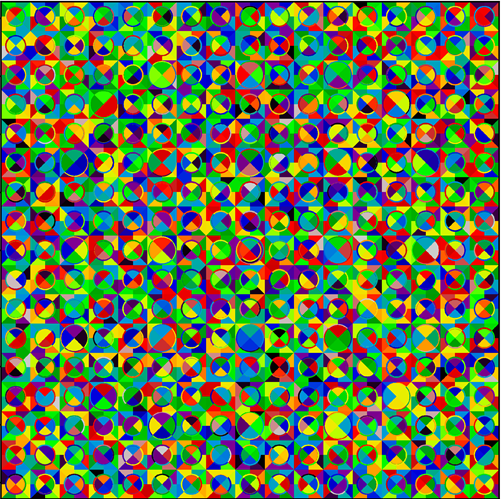
\includegraphics[width=\linewidth]{figures/moc_mesh.PNG}
		\caption{}
		\label{fig:cmfd-mesh-a}
	\end{subfigure}
	\begin{subfigure}{0.45\textwidth}
		\centering
		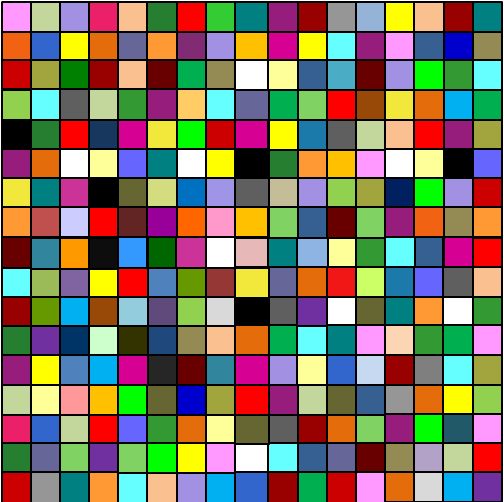
\includegraphics[width=\linewidth]{figures/cmfd_mesh.PNG}
		\caption{}
		\label{fig:cmfd-mesh-b}
	\end{subfigure}
	\caption[]{A depiction of the spatial mesh used in MOC (a) and CMFD (b) solvers. The mesh refinements correspond to those used in the final results for this thesis.}
	\label{fig:cmfd-mesh}
\end{figure}

For the energy condensation, the MOC calculations in this thesis use 70 energy groups whereas the CMFD solver uses 25 or less energy groups. The combination of coarse spatial mesh and coarse energy groups causes the CMFD problem size to be incredibly small in comparison with the MOC problem size. With the collapsed cross-sections on the coarse mesh, the CMFD transport equation looks very similar to the original multi-group transport equation and is given in Eq.~\ref{eqn:cmfd_transport}.
\begin{equation}
	\frac{1}{V_C^j} \sum_{g \in e} \left( \int\displaylimits_{S \in S_j} dS \, J_g\left(\mathbf{r}\right) \cdot \mathbf{n} \right) + \Sigma_{C,t}^{j,e} \phi_C^{j,e} = \frac{\chi_C^{j,e}}{k} \sum_{e'=1}^{E} \nu_C^{j, e'} \Sigma_{C,f}^{j,e'} \phi_C^{j,e'} + \sum_{e'=1}^E  \Sigma_{C,s}^{i, e' \rightarrow e} \phi_C^{j,e'}
	\label{eqn:cmfd_transport}
\end{equation}
Returning to the streaming term, the entire surface $S_j$ of CMFD cell $j$ is partitioned into a finite number of partial surfaces $H$ that form an interface between cell $j$ and exactly one other CMFD cell. This allows the total net current of CMFD cell $j$ to be defined in terms of the sum over net currents over these interfacial surfaces as given in Eq.~\ref{eqn:cmfd_partial_surface_currents}.
\begin{equation}
	\frac{1}{V_C^j} \sum_{g \in e} \sum_{h=1}^H \left( \int\displaylimits_{S \in S_{j,h}} dS \, J_g\left(\mathbf{r}\right) \cdot \mathbf{n} \right) + \Sigma_{C,t}^{j,e} \phi_C^{j,e} = \frac{\chi_C^{j,e}}{k} \sum_{e'=1}^{E} \nu_C^{j, e'} \Sigma_{C,f}^{j,e'} \phi_C^{j,e'} + \sum_{e'=1}^E  \Sigma_{C,s}^{i, e' \rightarrow e} \phi_C^{j,e'}
	\label{eqn:cmfd_partial_surface_currents}
\end{equation}
The integrated net current over each interfacial surface for an MOC group $g$ can be cast in terms of angular fluxes using the definition given in Eq.~\ref{eqn:net_current} to produce the relationship in Eq.~\ref{eqn:interfacial_current_def}.
\begin{equation}
	\int\displaylimits_{S_{j,h}} dS \, J_g\left(\mathbf{r}\right) \cdot \mathbf{n} =  \int\displaylimits_{S \in S_{j,h}} dS \, \int\displaylimits_{4 \pi} d\mathbf{\Omega} \, \psi_{g}(\mathbf{r},\mathbf{\Omega}) \left(\mathbf{\Omega} \cdot \mathbf{n} \right)
	\label{eqn:interfacial_current_def}
\end{equation}
Figure~\ref{fig:cmfd-contact-surface} shows the geometric relationship between a given MOC track and CMFD surfaces. This shows that the surface area penetrated on surface $S_{j,h}$ by track $t$ can be calculated as $\delta A_{t} / \left(\mathbf{\Omega} \cdot \mathbf{n}\right)$.
\begin{figure}[h!]
	\centering
	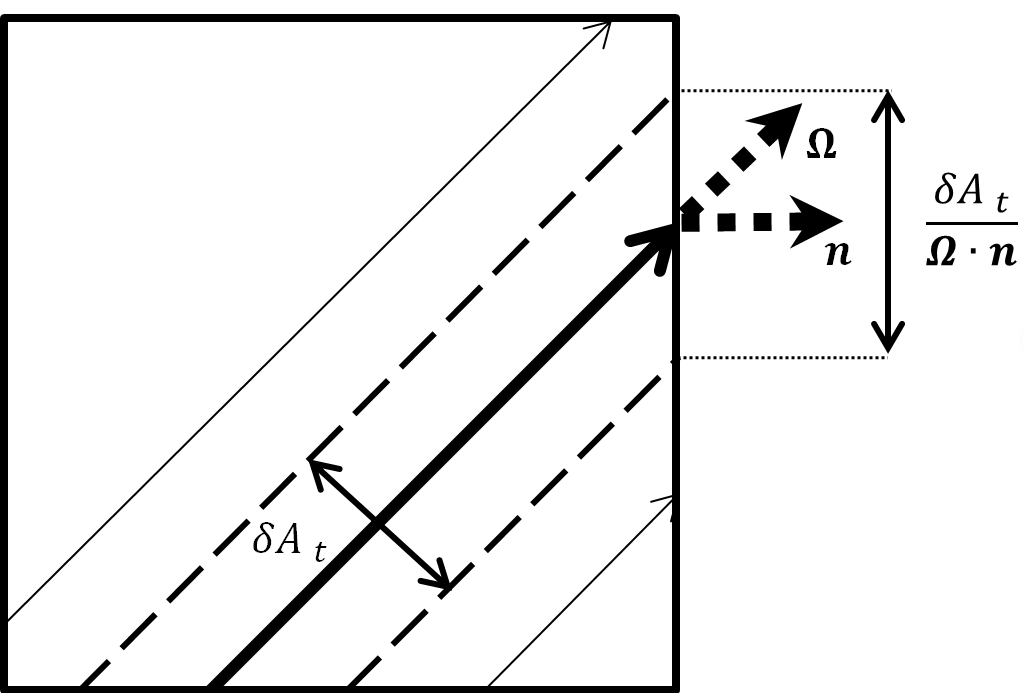
\includegraphics[width=0.5\linewidth]{figures/cmfd-contact-surface.PNG}
	\caption[]{A depiction of a CMFD surface with normal vector $\mathbf{n}$ being penetrated by a track with cross-sectional area $\delta A_{t}$ traveling in direction $\mathbf{\Omega}$. The area of the penetrated surface area is $\delta A_{t} / \left(\mathbf{\Omega} \cdot \mathbf{n}\right)$.}
	\label{fig:cmfd-contact-surface}
\end{figure}
With this geometric relationship in mind and factoring in angular weights from Eq.~\ref{eqn:weight-def}, the integrated net current over the interfacial surface can be calculated using Eq.~\ref{eqn:moc_net_current_calc}.
%\begin{equation}
%	\int\displaylimits_{S_{j,h}} dS \, J_g\left(\mathbf{r}\right) \cdot \mathbf{n} =  \sum_{(t,s) \in S_{j,h}} \frac{w_{t}}{\mathbf{\Omega} \cdot \mathbf{n}} \psi_{g}^{t,s}(s_{j,h}) \left(\mathbf{\Omega} \cdot \mathbf{n} \right)
%\end{equation}
\begin{equation}
	\int\displaylimits_{S \in S_{j,h}} dS \, J_g\left(\mathbf{r}\right) \cdot \mathbf{n} =  \sum_{(t,s) \in S_{j,h}} w_{i,t} \psi_{g}^{t,s}(s_{j,h})
	\label{eqn:moc_net_current_calc}
\end{equation}
Similar to the CMFD cross-sections, these currents are formed from the MOC calculation, so they are only approximate until convergence. Summing over all MOC groups $g$ within CMFD group $e$ gives a representation for the net current $\tilde{J}_{j,h,e}$ across surface $h$ of cell $j$ for CMFD group $e$ in Eq.~\ref{eqn:cmfd_partial_current}.
\begin{equation}
	\tilde{J}_{j,h,e} = \sum_{g \in e} \sum_{(t,s) \in S_{j,h}} w_t \psi_{g}^{t,s}(s_{j,h})
	\label{eqn:cmfd_partial_current}
\end{equation}
It is important to note that these estimates rely on angular fluxes. Since the entire angular flux vector is not stored explicitly, as discussed in Section~\ref{sec:moc-solve}, when a CMFD surface is encountered during the MOC transport sweep, the contribution of angular fluxes along the track to the net current on the CMFD surface must be tallied. This is usually a relatively cheap operation, not adding much work to the transport sweep. With these calculated currents, the new transport equation is given in Eq.~\ref{eqn:transport_partial_current_1}.
\begin{equation}
	\frac{1}{V_C^j} \sum_{h=1}^H \tilde{J}_{j,h,e} + \Sigma_{C,t}^{j,e} \phi_C^{j,e} = \frac{\chi_C^{j,e}}{k} \sum_{e'=1}^{E} \nu_C^{j, e'} \Sigma_{C,f}^{j,e'} \phi_C^{j,e'} + \sum_{e'=1}^E  \Sigma_{C,s}^{i, e' \rightarrow e} \phi_C^{j,e'}
	\label{eqn:transport_partial_current_1}
\end{equation}
With this new representation of neutron balance, it is possible to solve for new scalar fluxes. However, this is not in the form of an eigenvalue problem since the streaming term has no dependence on the scalar flux. Physically, a relationship is indeed expected between the streaming term and scalar flux since high scalar flux indicates dense neutron population and hence more leakage out of the volume. This concept is very similar to diffusion theory. Therefore, new terms are introduced that relate the current to the scalar flux via diffusion coefficients. This is shown in Eq.~\ref{eqn:cmfd_current_repr}.
\begin{equation}
	\frac{\tilde{J}_{j,h,e}}{A_{j,h}} = - u(j,h) \hat{D}_{j,e} \left(\phi_C^{I(j,h),e} - \phi_C^{j,e}\right) - \tilde{D}_{j,h,e} \left(\phi_C^{I(j,h),e} + \phi_C^{j,e}\right)
	\label{eqn:cmfd_current_repr}
\end{equation}
The function $u(j,h)$ is the \textit{sense} of the surface $h$ on cell $j$, $A_{j,h}$ is the area of surface $S_{j,h}$, $\hat{D}_{j,e}$ is the surface diffusion coefficient, and $\tilde{D}_{j,h,e}$ is the nonlinear corrected diffusion coefficient. The inspiration of the first term involving $\hat{D}_{j,e}$ comes from diffusion theory. Specifically it can be calculated using Eq.~\ref{eqn:surf_diff_coef} under a CMFD uniform mesh assumption
\begin{equation}
	\hat{D}_{j,h,e} = \frac{D_{j,e} D_{I(j,h),e}}{\Delta \mathbf{r}_h \left( D_{j,e} + D_{I(j,h),e} \right)}
	\label{eqn:surf_diff_coef}
\end{equation}
where $\Delta \mathbf{r}_h$ is the distance between the CMFD cell and the interfacial surface $h$, the function $I(j,h)$ computes the index of the neighboring CMFD cell of $j$ on surface $h$, and $D_{j,e}$ is the bulk diffusion coefficient of cell $j$ in group $e$. Due to the uniform mesh assumption, the distance between the centroid of cell $j$ and surface $h$ is the same as that of the neighboring cell $I(j,h)$. In this thesis, the uniform mesh assumption is imposed, but a more general treatment is possible. The bulk diffusion coefficients are defined in Eq.~\ref{eqn:cmfd_diff_coef}, with motivation from how diffusion coefficients are calculated in common nodal diffusion theory.
\begin{equation}
	D_{j,e} = \frac{\sum_{i \in j} \sum_{g \in e} \frac{1}{3\Sigma_{t}^{i, g}} \overline{\phi_{i,g}} V_i}{\sum_{i \in j} \sum_{g \in e} \overline{\phi_{i,g}} V_i}
	\label{eqn:cmfd_diff_coef}
\end{equation}
The sense $u(j,h)$ is calculated by Eq.~\ref{eqn:sense} where $\mathbb{1}$ is just the vector of ones in three dimensions and $\mathbf{n}_{j,h}$ is the normal vector of surface $S_{j,h}$. For a Cartesian uniform mesh, the sense is $+1$ if the surface is a positive $x$, $y$, or $z$ surface and $-1$ if it is a negative $x$, $y$, or $z$ surface.
\begin{equation}
u(j,h) = \frac{\mathbb{1} \cdot \mathbf{n}_{j,h}}{|\mathbb{1} \cdot \mathbf{n}_{j,h}|}
\label{eqn:sense}
\end{equation}
Lastly, the corrected diffusion coefficients $\tilde{D}_{j,h,e}$ are computed based on the relationship in Eq.~\ref{eqn:cmfd_current_repr} for fluxes computed after the MOC transport sweep and before the CMFD solve. This makes the CMFD calculation consistent with the MOC calculation at convergence~\cite{smith1983cmfd}. The calculation of the corrected diffusion coefficients therefore follows Eq.~\ref{eqn:cmfd_corr_dif_coef} where $\tilde{\phi}_C^{j,e}$ are the CMFD cell-averaged scalar fluxes calculated from the MOC iteration with the tilde indicating the quantity comes from the MOC calculation and does not change throughout the CMFD iterations.
\begin{equation}
	\tilde{D}_{j,h,e} = \frac{-u(j, h) \hat{D}_{j,h,e} \left(\tilde{\phi}_C^{I(j,h),e} - \tilde{\phi}_C^{j,e}\right) - \frac{\tilde{J}_{j,h,e}}{A_{j,h}}}{\tilde{\phi}_C^{I(j,h),e} + \tilde{\phi}_C^{j,e}}
	\label{eqn:cmfd_corr_dif_coef}
\end{equation}
Returning to balance equation and inserting the relationship for net current yields the new balance equation given in Eq.~\ref{eqn:cmfd_final_balance}.
\begin{equation}
\begin{split}
	\frac{1}{V_C^j} \sum_{h=1}^H A_{j,h} \left( - u(j, h) \hat{D}_{j,e} \left(\phi_C^{I(j,h),e} - \phi_C^{j,e}\right) - \tilde{D}_{j,h,e} \left(\phi_C^{I(j,h),e} + \phi_C^{j,e}\right) \right) + \Sigma_{C,t}^{j,e} \phi_C^{j,e} = \\
	\frac{\chi_C^{j,e}}{k} \sum_{e'=1}^{E} \nu_C^{j, e'} \Sigma_{C,f}^{j,e'} \phi_C^{j,e'} + \sum_{e'=1}^E  \Sigma_{C,s}^{i, e' \rightarrow e} \phi_C^{j,e'}
\end{split}
\label{eqn:cmfd_final_balance}
\end{equation}

\section{Solving the CMFD Equations for MOC Acceleration}
The CMFD balance equation in Eq.~\ref{eqn:cmfd_final_balance} represents a physically equivalent system to solve the transport equation as the MOC balance equation in Eq.~\ref{eqn:angular-flux-var-disc}. Re-arranging terms in the balance equation and grouping by scalar flux yields the relationship in Eq.~\ref{eqn:cmfd_balance_grouped}.
\begin{equation}
	\begin{split}
		\left[\Sigma_{C,t}^{j,e} V_C^j + \sum_{h=1}^H A_{j,h} \left(u(j,h) \hat{D}_{j,e} - \tilde{D}_{j,h,e} \right) \right] \phi_C^{j,e} - \sum_{h=1}^H A_{j,h} \left( \tilde{D}_{j,h,e} + u(j,h) \hat{D}_{j,e} \right) \phi_C^{I(j,h),e} & \\ - \sum_{e'=1}^E  \Sigma_{C,s}^{i, e' \rightarrow e} V_C^j \phi_C^{j,e'} =
		\frac{\chi_C^{j,e}}{k} \sum_{e'=1}^{E} \nu_C^{j, e'} \Sigma_{C,f}^{j,e'} V_C^j \phi_C^{j,e'} & \\
	\end{split}
	\label{eqn:cmfd_balance_grouped}
\end{equation}
This can be written in terms of a matrix eigenvalue problem by defining a scalar flux vector $\Phi_C$ which incorporates all of the CMFD cell-averaged scalar fluxes $\phi_C^{j,e}$, a loss matrix $A$, and a multiplicative matrix $M$ in Eq.~\ref{eqn:cmfd_eigenvalue_problem}.
\begin{equation}
	A \Phi_C = \frac{1}{k} M \Phi_C
	\label{eqn:cmfd_eigenvalue_problem}
\end{equation}
This can be related to a regular eigenvalue problem by taking the inverse of $A$ as
\begin{equation}
	A^{-1} M \Phi_C = k \Phi_C.
\end{equation}
Any common eigenvalue solver can be used to solve this system. In this thesis, simple power iteration is employed. More details on practical implementation aspects of CMFD in this thesis are given in Chapter~\ref{chap:cmfd-optimize}.

Once the CMFD equations are solved, the solution is used to update MOC fluxes, hence producing a new source on the next iteration. The updating of MOC fluxes is the prolongation step of the CMFD process. There are a variety of ways for which the CMFD fluxes can be updated. One simple approach is just updating all MOC fluxes in source region $i$ and MOC group $g$ encompassed by CMFD cell $j$ and CMFD group $e$ by applying Eq.~\ref{eqn:cmfd_simple_prolongation}:
\begin{equation}
\phi_{i,g}^{\text{new}} = \phi_{i,g}^{\text{old}} \, \frac{\phi_{C, \, \text{new}}^{j,e}}{\phi_{C, \, \text{old}}^{j,e}}
\label{eqn:cmfd_simple_prolongation}
\end{equation}
where $\phi_{i,g}^{\text{new}}$ refers to the updated MOC flux after prolongation, $\phi_{i,g}^{\text{old}}$ refers to the MOC flux before prolongation, $\phi_{C, \, \text{old}}^{j,e'}$ refers to the CMFD cell-averaged flux at the start of the CMFD solution (calculated directly from the MOC fluxes), and $\phi_{C, \, \text{new}}^{j,e'}$ refers to the CMFD cell-averaged flux at convergence of the CMFD solution. It is important to ensure that both new and old scalar fluxes are normalized in the same manner.

Updating the MOC fluxes with the CMFD solution allows convergence to be greatly accelerated, quickly capturing the flux shape over the coarse mesh. In addition, the computational cost of fully converging the CMFD solution is small in comparison with just one MOC transport sweep. Therefore, using the process laid out at the beginning of this chapter in Figure~\ref{fig:multigrid-cmfd}, the CMFD equations are formed and solved after every transport sweep. This process for solving the MOC neutron transport eigenvalue problem with CMFD acceleration is detailed in Alg.~\ref{alg:moc-cmfd-eigenvalue-solve}.

\begin{algorithm}
	\caption[MOC Eigenvalue Solver with CMFD Acceleration]{OpenMOC Eigenvalue Solver with CMFD Acceleration}
	\label{alg:moc-cmfd-eigenvalue-solve}
	\begin{algorithmic}[1]
		\Procedure{computeEigenvalue}{$geometry$, $tracks$, $N$}
		\State Implicitly define $F$, $S$, $H$, $D$, and $T$ from $geometry$ \Comment{Definitions in Chapter~\ref{chap:moc}}
		\State $\boldsymbol{\phi} \gets \mathbb{1}$ \Comment{Initialize scalar fluxes to all ones}
		\State $\boldsymbol{\psi} \gets 0$ \Comment{\parbox[t]{.4\linewidth}{Initialize angular fluxes to zeros (only boundary stored)}}
		\State $k \gets 1$ \Comment{Initialize the eigenvalue to 1}
		\State $\boldsymbol{\phi} \gets \boldsymbol{\phi} \, / \, \left(\mathbb{1}^T F \boldsymbol{\phi}\right)$ \Comment{Normalize by total fission source}
		\While{not converged}
		\State $\mathbf{q} \gets \frac{1}{4\pi} \left(S \boldsymbol{\phi} + \frac{1}{k} F \boldsymbol{\phi} \right)$ \Comment{Compute neutron sources}
		\State \parbox[t]{.3\linewidth}{$\boldsymbol{\psi} \gets T^{-1} H D^{-1} \mathbf{q}$ \\ $\mathbf{p} \gets W \boldsymbol{\psi}$} \Comment{\parbox[t]{.5\linewidth}{Transport Sweep: these equations are solved simultaneously for computational efficiency. Currents on CMFD surfaces are tallied. Only angular fluxes on the boundary are explicitly stored.}}
		\State $\boldsymbol{\phi} \gets D^{-1}\mathbf{q} + D^{-1}
		\mathbf{p}$ \Comment{Scalar fluxes computed from tally $\mathbf{p}$}
		\State Form CMFD matrices $A$ and $M$ \Comment{\parbox[t]{.4\linewidth}{Defined by Eq.~\ref{eqn:cmfd_balance_grouped} and Eq.~\ref{eqn:cmfd_eigenvalue_problem} \\ (\textbf{restriction})}}
		\State Compute CMFD scalar fluxes $\Phi_C$ \Comment{Defined by Eq.~\ref{eqn:cmfd_scalar_fluxes} (\textbf{restriction})}
		\State $\Phi_C \gets \Phi_C \, / \, \left(\mathbb{1}^T M \Phi_C\right)$ \Comment{Normalize by total CMFD fission rate}
		\State $\tilde{\Phi}_C \gets \Phi_C$ \Comment{Save pre-CMFD scalar fluxes}
		\While{not converged}
			\State $\Phi_C \gets A^{-1} M \Phi_C$ \Comment{\parbox[t]{.5\linewidth}{Compute inverse with a linear solver \\ (Gauss-Seidel)}}
			\State $k \gets \mathbb{1}^T M \Phi_C$ \Comment{\parbox[t]{.5\linewidth}{Implicitly computing \\ $\left(\mathbb{1}^T M A^{-1} M \Phi_C\right) \, / \, \left(\mathbb{1}^T M \Phi_C\right)$}}
			\State $\Phi_C \gets \Phi_C \, / \, \left(\mathbb{1}^T M \Phi_C\right)$ \Comment{Normalize by total CMFD fission rate}
		\EndWhile
		\State \parbox[t]{.4\linewidth}{Update $\boldsymbol{\phi}$ by interpolating the \\ ratio of $\Phi_C$ and $\tilde{\Phi}_C$} \Comment{This is the \textbf{prolongation} step}
		\State $\boldsymbol{\phi} \gets \boldsymbol{\phi} \, / \, \left(\mathbb{1}^T F \boldsymbol{\phi}\right)$ \Comment{Normalize by total fission source}
		\EndWhile
		\State \textbf{return} $\boldsymbol{\phi}$ and $k$ \Comment{Return scalar fluxes and the eigenvalue}
		\EndProcedure
	\end{algorithmic}
\end{algorithm}

\newpage
\vfill
\begin{highlightsbox}[frametitle=Highlights]
	\begin{itemize}
		\item CMFD is a variant of multigrid methods, with a restriction step to reduce the problem size to a coarse CMFD mesh and a prolongation step to interpolate the coarse mesh CMFD solution onto the fine MOC mesh.
		\item The CMFD equations are based in diffusion theory, with currents defined from the MOC solution to ensure consistency between the MOC and CMFD equations.
		\item Solving the CMFD system equations is computationally cheap in comparison with the solution of the fine mesh MOC equations.
		\item CMFD accelerates MOC convergence by being able to capture global behavior quickly on the coarse mesh.
	\end{itemize}
\end{highlightsbox}
\vfill
\chapter{The BEAVRS Benchmark}
\label{chap:beavrs}

The main results presented in this thesis are based on models formed from the BEAVRS benchmark~\cite{horelik2013beavrs}. This chapter introduces the BEAVRS benchmark in Section~\ref{sec:beavrs-intro}, including a description of alteration made to the benchmark. Section~\ref{sec:beavrs-xs-gen} describes how cross-sections are generated for the benchmark. Finally, Section~\ref{sec:beavrs-models} details the particular models formed from cutouts of the BEAVRS model and, in some cases, replication of the cutouts.

%%%%%%%%%%%%%%%%%%%%%%%%%%%%%%%%%%%%%%%%%%%%%%%%%%%%%%%%%%%%%%%%%%%%%%%%%%%%%%%%
\section{Introduction to the BEAVRS Benchmark}
\label{sec:beavrs-intro}

The BEAVRS benchmark~\cite{horelik2013beavrs} was released in 2013, representing a Westinghouse 4-loop nuclear power reactor. This reactor is representative of common \ac{PWR} designs in the United States. The benchmark contains core loadings and detector measurements for the first two cycles of operation, but this thesis concentrates on \ac{HZP} simulations at the beginning of the first cycle in an all rods out configuration.

The reactor contains 193 fuel assemblies. Each assembly contains a $17 \times 17$ lattice of fuel rods, guide tubes, and instrument tubes. The pin-pitch is 1.26 cm inside each assembly. All fuel rods within the same assembly contain uranium of the same enrichment. In the first cycle, three uranium enrichments are used: 1.6\%, 2.4\%, and 3.1\%. Wet annular burnable absorbers are present throughout the core to flatten the power distribution. The active fuel height is 365.76 cm. A radial description of the core is shown in Figure~\ref{fig:beavrs-assembly-enrichment}.

\begin{figure}[h!]
	\centering
	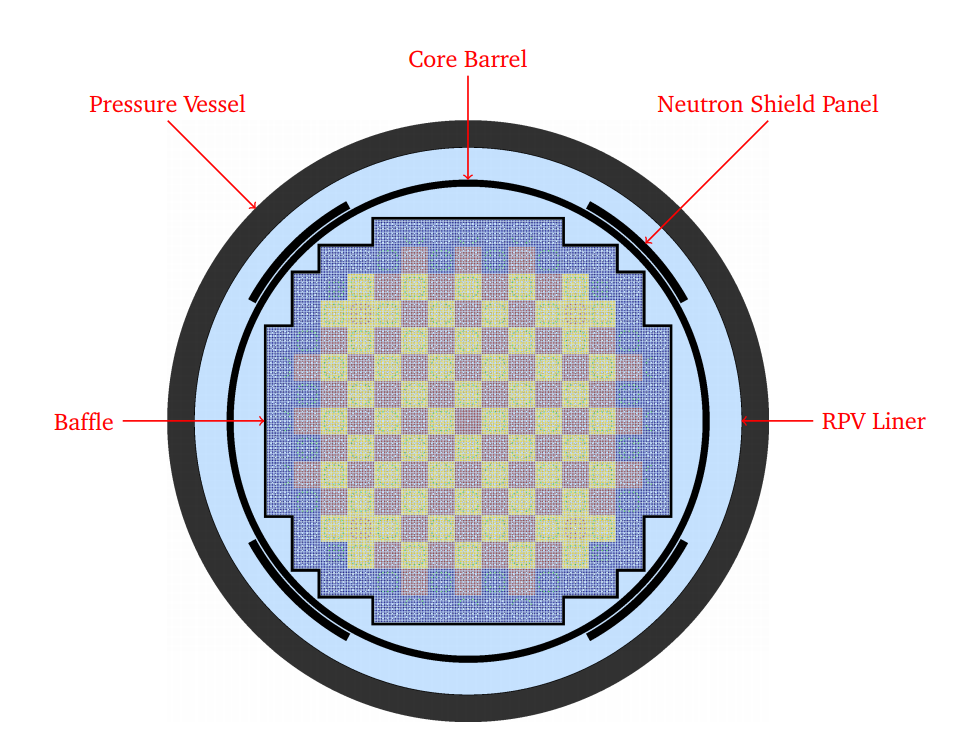
\includegraphics[width=\linewidth]{figures/beavrs-visual/beavrs-assembly-enrichment.png}
	\caption{A radial illustration of the BEAVRS benchmark with fuel pins colored by enrichment.}
	\label{fig:beavrs-assembly-enrichment}
\end{figure} 

The goal of this thesis is to simulate the BEAVRS benchmark using the explicit detail provided in the BEAVRS specification. However, in order to conduct uniform axial mesh refinement studies, the axial heights of material regions are altered such that each discontinuity occurs at an even number (in cm). The top and bottom grid spacers in the BEAVRS benchmark were defined to be 5.72 cm with intermediate grid spacers 3.36 cm. These lengths were altered to 6.0 cm and 2.0 cm respectively. The starting height of the grid spacers were rounded to the nearest even integer. All other $z$-heights in the geometry were similarly rounded to the nearest integer. The altering of axial heights allows regions to be formed which all have the same axial height, which can simplify sensitivity analysis. While these alterations do change the benchmark slightly -- and therefore also change the computed solutions -- these solutions are still representative of a realistic \ac{PWR} problem.

Although the BEAVRS model is defined inside a cylindrical geometry, a rectangular bounding geometry is often necessary in \ac{MOC} methods for cyclic tracking. Therefore, the BEAVRS model is modeled with a rectangular prism bounding the geometry. In the radial plane, the bounding dimensions are square with length equal to 17 assembly widths. Since the BEAVRS model has a maximum of 15 assemblies along each $x$ and $y$ direction, this allows at least one assembly of radial reflector to be modeled outside the core. In addition, the corners have very deep water reflectors. In the axial direction, the BEAVRS benchmark is modeled with 400 cm height, allowing approximately 20 cm of axial reflector in each direction. Vacuum boundaries are assumed on all surfaces. 


%%%%%%%%%%%%%%%%%%%%%%%%%%%%%%%%%%%%%%%%%%%%%%%%%%%%%%%%%%%%%%%%%%%%%%%%%%%%%%%%
\section{Cross-Section Generation}
\label{sec:beavrs-xs-gen}

In this thesis, the same 70 group cross-section library is used for all results involving the BEAVRS benchmark or cutouts of the BEAVRS benchmark except for the rod insertion studies. A separate 70 group cross-section library was formed for rod insertion studies in order to form accurate cross-sections for control rod materials. In this section, the process used to form cross-sections is thoroughly discussed.

Using the OpenMC Monte Carlo code, reaction rate tallies are generated for each unique material. These allow for the computation of multi-group cross-sections with the methodology discussed in Chapter~\ref{chap:mgxs} using the \texttt{mgxs} package implemented by Boyd~\cite{boyd2017thesis}. The 70 group library is formed from an OpenMC simulation of the full core BEAVRS benchmark. The Monte Carlo simulation used 400 batches (300 inactive, 100 active) with $2 \times 10^8$ particles per batch. The in-scatter transport correction described in Section~\ref{sec:transport-correction} is applied to the cross-sections using anisotropic scattering tallies. Note that using these tallies to form the transport correction introduces approximation since the true tallies should involve angular fluxes rather than scalar fluxes. Since the anisotropic current tallies could vary significantly between core and outer reflector regions, the water is split into two materials for which cross-sections are independently formed: core water and outer reflector water. In addition, a third water material is also formed near the support plate nozzle as the isotopic composition differs due to boron concentration. A plot of the BEAVRS benchmark colored by unique material region is shown in Figure~\ref{fig:beavrs-materials-radial}. In addition an axial plot of the materials is shown in Figure~\ref{fig:beavrs-materials-axial}. Similarly the radial and axial material plots of a 1.6\% enriched fuel assembly are shown in Figure~\ref{fig:beavrs-single-assembly-materials-radial} and Figure~\ref{fig:beavrs-single-assembly-materials-axial}, respectively.


\begin{figure}[h!]
	\centering
	\includegraphics[width=\linewidth]{figures/beavrs-visual/materials-beavrs-radial.jpg}
	\caption{A radial view of the BEAVRS benchmark with regions colored by material.}
	\label{fig:beavrs-materials-radial}
\end{figure} 

\begin{figure}[h!]
	\centering
	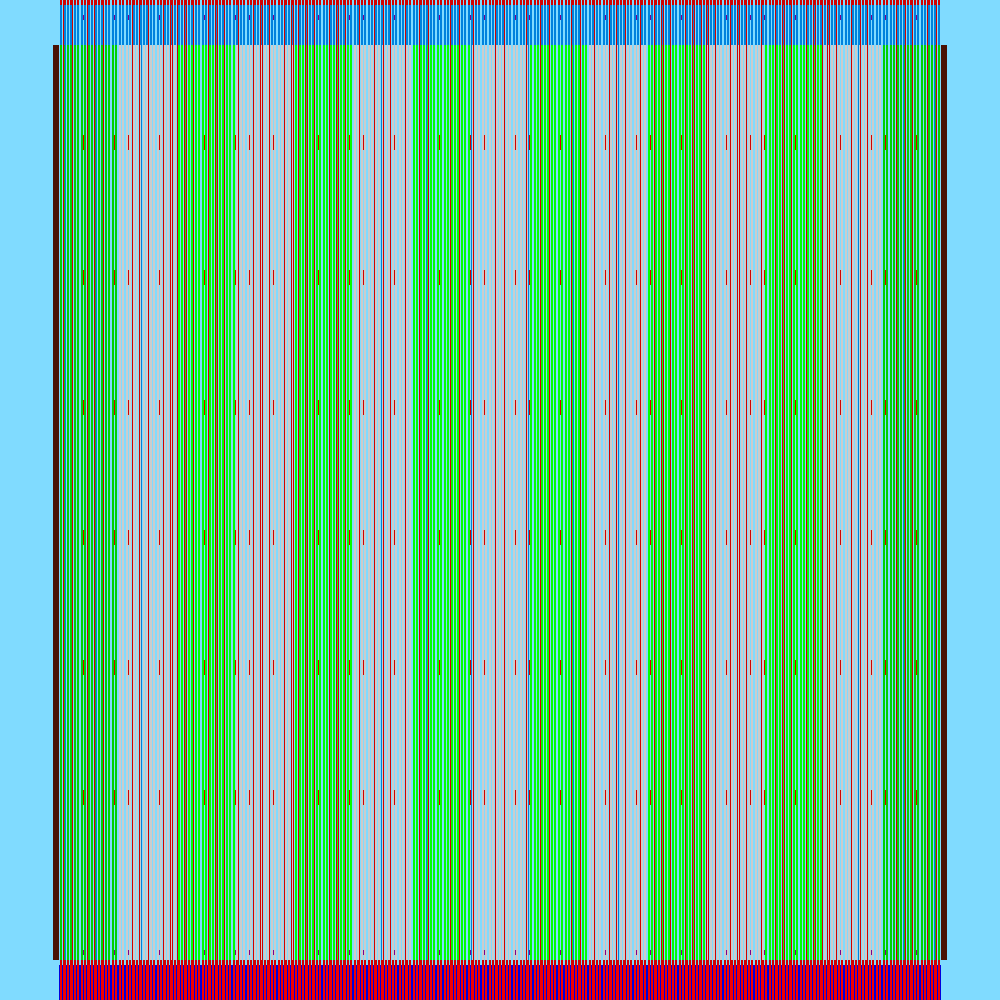
\includegraphics[width=\linewidth]{figures/beavrs-visual/materials-beavrs-axial.jpg}
	\caption{An axial view of the BEAVRS benchmark with regions colored by material.}
	\label{fig:beavrs-materials-axial}
\end{figure} 

\begin{figure}[h!]
	\centering
	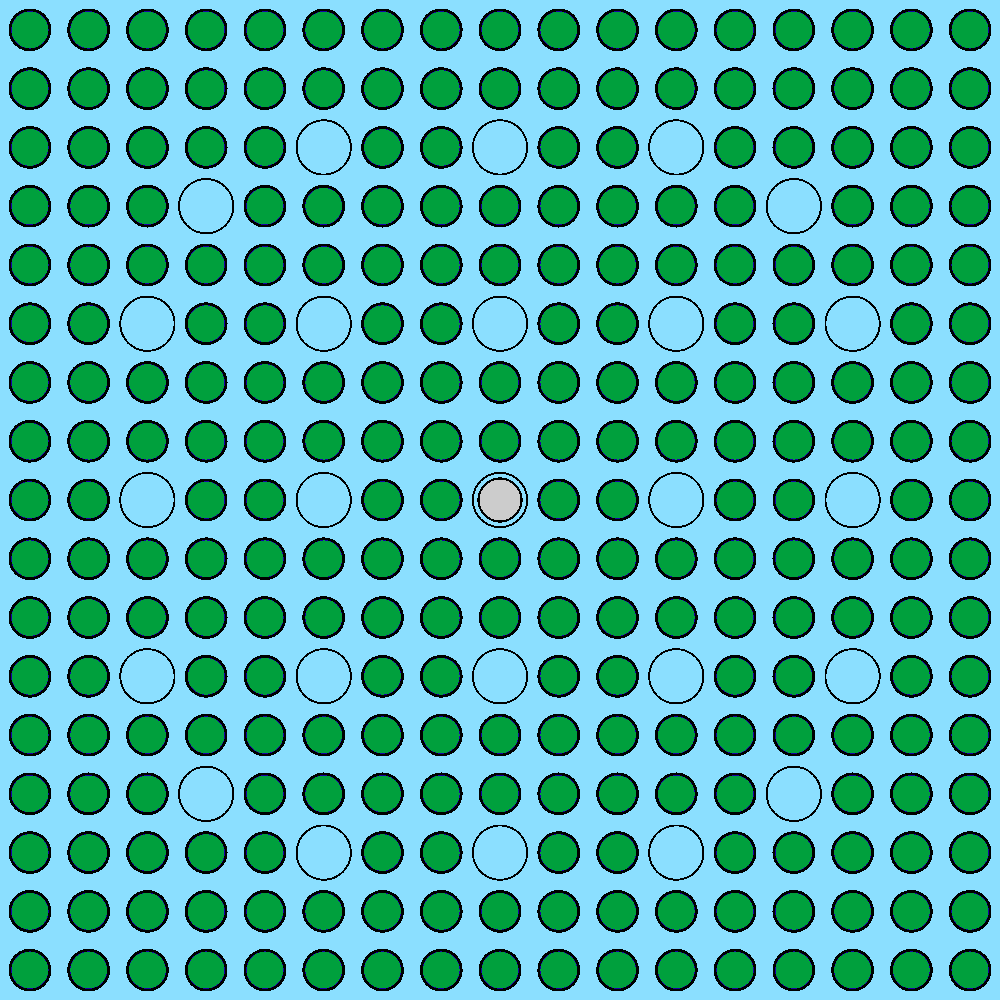
\includegraphics[width=0.65\linewidth]{figures/beavrs-visual/materials-single-assembly-radial.png}
	\caption{A radial view of the 1.6\% enriched fuel assembly in the BEAVRS benchmark with regions colored by material.}
	\label{fig:beavrs-single-assembly-materials-radial}
\end{figure} 

\begin{figure}[h!]
	\centering
	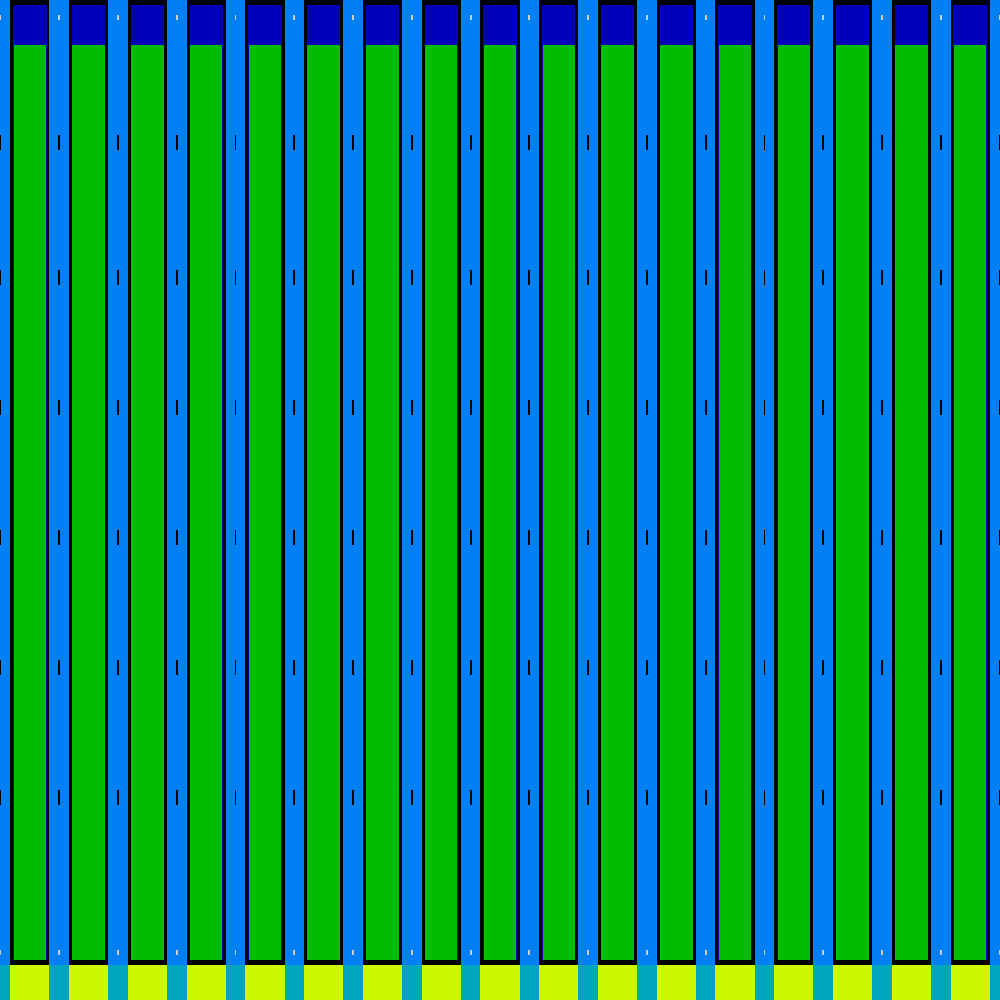
\includegraphics[width=0.65\linewidth]{figures/beavrs-visual/materials-single-assembly-axial.png}
	\caption{An axial view of 1.6\% enriched fuel assembly in the BEAVRS benchmark with regions colored by material.}
	\label{fig:beavrs-single-assembly-materials-axial}
\end{figure} 



\clearpage

The computed cross-sections were compared with CASMO-4 cross-sections and significant differences were found in the transport correction for water. In preliminary tests, the CASMO-4 multi-group cross-sections for core water were also able to much more accurately simulate the gross fission distribution. Therefore, instead of solely using the OpenMC \texttt{mgxs} cross-sections for core water which had an inaccurate transport correction, or solely using CASMO-4 cross-sections which are generated for more general problems, a new cross-section set was formed specifically for core water. Since CASMO-4 is a lattice physics code, it is designed to have accurate estimates of core water cross-sections. Therefore, the transport correction from CASMO-4 is used to modify the cross-sections formed by the OpenMC \texttt{mgxs} package. Specifically, the transport cross-section $\Sigma_{tr}^g$ for group $g$ is formed by computing
\begin{equation}
\Sigma_{tr}^g = \Sigma_{a}^g + \eta \left( \Sigma_{t}^g - \Sigma_{a}^g \right)
\end{equation}
where $\Sigma_{a}^g$ and $\Sigma_{t}^g$ are the associated absorption and total cross-sections formed by \texttt{mgxs}, respectively. The factor $\eta$ is computed by
\begin{equation}
\eta = \frac{\Sigma_{tr}^{g, \textbf{CASMO}} - \Sigma_{a}^{g, \textbf{CASMO}}}{\Sigma_{t}^{g, \textbf{CASMO}} - \Sigma_{a}^{g, \textbf{CASMO}}}
\end{equation}
where the \textbf{CASMO} superscript denotes CASMO-4 cross-sections. It is important to note that this is only done for core water. All other materials use the cross-sections formed directly from the \texttt{mgxs} package in OpenMC.

%%%%%%%%%%%%%%%%%%%%%%%%%%%%%%%%%%%%%%%%%%%%%%%%%%%%%%%%%%%%%%%%%%%%%%%%%%%%%%%%
\section{Description of BEAVRS Models}
\label{sec:beavrs-models}

All models which are simulated in this thesis are derived from cutouts of the BEAVRS benchmark with 70 group cross-sections. In past presentations the, 3D \ac{MOC} solver implemented in this thesis has been verified on a variety of simpler, conventional reactor physics models~\cite{physor2016shaner, physor2016otf}. The BEAVRS benchmark represents a far more computationally demanding challenge, especially with a 70 group cross-section library. Cutouts are formed in order to evaluate smaller problems which are representative of computational performance or physical behavior of the large full core problem.

\subsection{Full Core 3D Model}
\label{sec:beavrs-3D}

The first model is just the BEAVRS model incorporating all the details discussed in previous sections. The simulation of this model directly corresponds with the OpenMC simulations from which the cross-sections are derived. The objective of this thesis is to accurately simulate this model. However, due to the large computational cost of simulating this model, only minimal tests can be conducted. Therefore, smaller cutouts are formed which are more computationally feasible in order to test computational and physical behavior before running the 3D full core case.


\subsection{Full Core 2D Model}
\label{sec:beavrs-2D}

A 2D extruded cutout of the reactor is formed in order to determine the physical behavior of the BEAVRS model in the radial direction. This cutout is taken from an 10 cm axial interval over which there are no grid spacers. Reflective boundary conditions are placed on the top and bottom of the problem. While this model lacks any axial variation, it still contains all radial detail. Due to the lack of axial detail, 2D \ac{MOC} and 3D \ac{MOC} simulations with sufficient parameter refinement should produce equivalent solutions. Only this model and the full core 3D model contain the full radial water reflector. Therefore, this model is very useful in determining the effect of large radial water reflectors. 

\subsection{Single Assembly Model}
\label{sec:beavrs-single-assembly}

A single assembly model is formed which represents the full axial detail of a single 1.6\% enriched fuel assembly. While this model lacks radial water reflectors, it contains the full axial detail fo the full core problem, including grid spacers. Outside the core, full geometrical detail is also captured including support plate nozzles and, most notably, water reflectors of approximately 20 cm above and below the fuel. Reflective boundaries are placed on the $x$ and $y$ boundaries. Physically, this is equivalent to an infinite 2D lattice of 1.6\% enriched fuel assemblies. Vacuum boundaries remain on the top and bottom of this model. Since this problem is significantly less computationally expensive than the full core models (both 2D and 3D), it allows rigorous parameter refinement and convergence studies.

\subsection{Truncated Single Assembly Model}
\label{sec:trunc-single-assembly}

In addition to the single assembly model, a truncated single assembly model is also formed which contains all the detail of the single assembly model, but without the axial water reflectors. Specifically, 20 cm are removed from both the bottom and top of the model, resulting in a model that only covers the active fuel and is 360 cm tall. Axial boundaries still have vacuum boundary conditions. Comparison with the single assembly model described in Section~\ref{sec:beavrs-single-assembly} allows for the effect of axial water reflectors to be directly tested.

\subsection{SDSA Model}
\label{sec:sdsa}

The Single Domain Single Assembly (SDSA) model is formed for rigorous performance testing. It represents a 20 cm tall cutout within the single assembly model which contains no grid spacers. Reflective boundary conditions are imposed on all surfaces. Since this problem is far reduced in size, it allows for rigorous performance testing. In Chapter~\ref{chap:domain-decomposition}, spatial domain decomposition is introduced in which the geometry is split into equal sized domains in which each computational node is expected to handle one domain. When simulating the BEAVRS benchmark with domain decomposition, the expected domain size is the size of the SDSA model. Therefore, this model allows for realistic on-node performance characterization of the BEAVRS benchmark without needing to run the large full core problem.

\subsection{Short Single Assembly Model}
\label{sec:short-single-assembly}

Similar to the SDSA model, a short single assembly model is created which allows for studies at far reduced computational cost. This model is the same as the SDSA model except it is only 10 cm in axial height and contains 3.1\% enriched fuel. This enrichment is the highest enrichment found in the cycle 1 BEAVRS model. The higher enriched fuel allows for slightly larger gradients with a flux peak in the moderator. The primary focus of this model is to test in-core radial mesh sensitivity.


\subsection{Rodded Single Assembly Model}
\label{sec:rodded-single-assembly}

The rodded single assembly model is the only model which uses a geometry not explicitly found in the full core 3D BEAVRS model. The model is constructed in the same way as the single assembly model described in Section~\ref{sec:beavrs-single-assembly}, but with 3.1\% enriched fuel and with all rods inserted at 100 steps -- covering approximately half of the active fuel height. This large control rod insertion causes significant gradients within the axial scalar flux distribution, allowing for robust testing of 3D \ac{MOC} on problems with significant axial variation.

As mentioned previously, this model uses a separate cross-section library. Instead of simulating the all rods out configuration, which lacks control rods within the core, the single assembly model is explicitly simulated in OpenMC to form cross-section estimates. This allows reasonable estimates of control rod material cross-sections.


\newpage
\vfill
\begin{highlightsbox}[frametitle=Highlights]
	\begin{itemize}
		\item The BEAVRS benchmark represents a traditional \ac{PWR} reactor encompassing all relevant radial and axial detail
		\item The BEAVRS model is simulated within a radially square bounding box, leading to large corner reflector regions
		\item A 70 group cross-section library is formed through direct simulation of the BEAVRS benchmark in Monte Carlo using the OpenMC \texttt{mgxs} package with a combination of CASMO-4 and in-scatter transport corrections
		\item Cutouts of the BEAVRS model allow for physics and computational behavior to be tested with much lower computational cost
		\item A rodded single assembly model is created to test the effect of large axial variation, for which a separate cross-section library is generated in order to accurately capture control rod properties
		
	\end{itemize}
\end{highlightsbox}
\vfill


%\chapter{Simulation Workflow}
\label{chap:workflow}

%%%%%%%%%%%%%%%%%%%%%%%%%%%%%%%%%%%%%%%%%%%%%%%%%%%%%%%%%%%%%%%%%%%%%%%%%%%%%%%%
\section{A Simulation Triad}
\label{chap4:triad}

This thesis investigates Monte Carlo as a means to generate multi-group cross sections for fine mesh transport codes. This work required the development of a ``simulation triad'' encompassing three primary codes as illustrated in Fig.~\ref{fig:chap4-simulation-triad}. First, the OpenMC Monte Carlo code~\cite{romano2013openmc} was utilized to generate multi-group cross sections. Second, the \ac{MGXS} were used by the OpenMOC \ac{MOC} code~\cite{boyd2014openmoc} for deterministic multi-group transport calculations. Finally, the OpenCG library~\cite{boyd2015opencg} enabled the processing and transfer of tally data on combinatorial geometry (CG) meshes between OpenMC and OpenMOC. In addition, a significant amount of infrastructural code was developed to process the results produced by OpenMC and OpenMOC. The results in this thesis may be most easily reproduced with the versions of OpenMC, OpenMOC and OpenCG itemized in Tab.~\ref{table:chap4-git-shas}.

\begin{table}[hb!]
  \centering
  \caption[OpenMC, OpenMOC and OpenCG Git SHA-1 hashes]{The Git SHA-1 commit hashes for each code used in this thesis.}
  \small
  \label{table:chap4-git-shas} 
  \vspace{6pt}
  \begin{tabular}{l c c}
  \toprule
  \rowcolor{lightgray}
  {\bf Code} &
  {\bf Date [MM-DD-YYYY]} &
  {\bf Git Commit SHA-1} \\
  \midrule
  OpenMC & 05-30-2016 & 698c223482a7d5f5df4dc83eeed65d99a2e52fbf \\
  OpenMOC\footnotemark & 05-29-2016 & b09e66be269703ca0a08d7a6afced1bc5984112a \\
  OpenCG & 05-14-2016 & 2c5e8f92f501d076f4ed06b70b09684a411b06b9 \\
  \bottomrule
\end{tabular}
\end{table}

\footnotetext{OpenMOC was compiled with double precision floating point arithmetic.}

\begin{figure}[h]
  \centering
  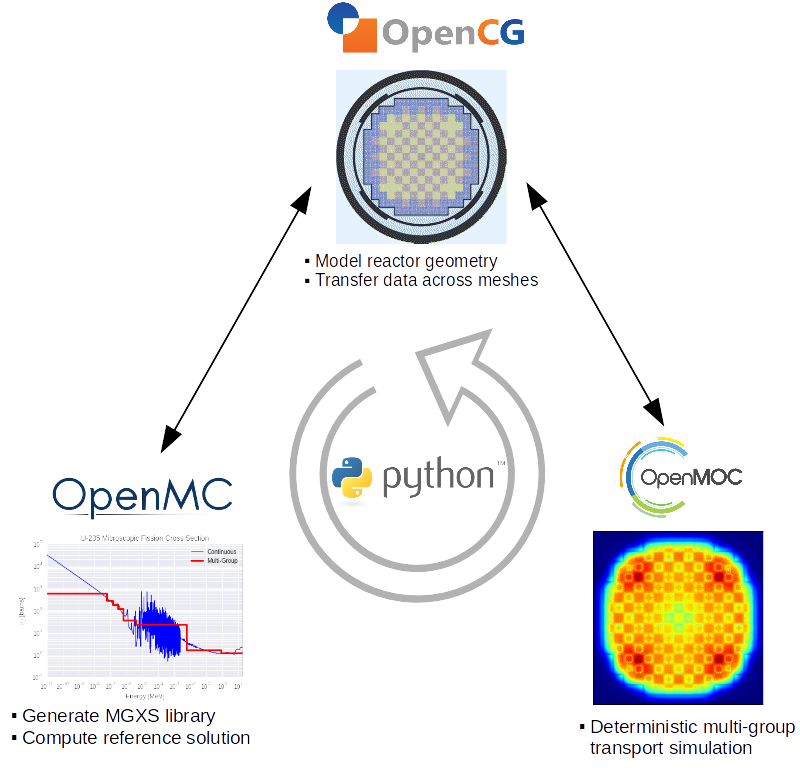
\includegraphics[width=0.8\linewidth]{figures/workflow/triad/simulation-triad}
\caption[A simulation triad of OpenMC, OpenMOC and OpenCG]{A simulation triad consisting of the OpenMC, OpenMOC and OpenCG codes ``glued'' together with Python formed the foundation for this thesis research.}
\label{fig:chap4-simulation-triad}
\end{figure}

This chapter describes the author's contributions to each component code in the simulation triad to support the objectives of this thesis -- namely, the evaluation of intrinsic bias in \ac{MGXS} for fine mesh transport (Chaps.~\Crefrange{chap:biases}{chap:sph}), and the development of a novel metholodogy for spatial homgenization based on unsupervised clustering (Chaps.~\Crefrange{chap:benchmarks}{chap:unsupervised}). An overview of the OpenMC, OpenMOC, and OpenCG codes, along with the features added to each code to support this thesis, are presented in Secs.~\ref{sec:chap4-openmc},~\ref{sec:chap4-openmoc}, and~\ref{sec:chap4-opencg}, respectively.

%The infrastructural code framework was developed using the Python programming language due to its flexibility and ease of use, as well as its extensive ecosystem of open source packages for high-performance data analysis.

%second paragraph: big data -> perhaps this should be in the motivation above?
%-explain/assume the need to tally across each spatial mesh zone
%-need to process large amounts of tally data
%-BEAVRS core figures for motivation
%-bulletize requirements?
%  -\# nuclides, \# tally regions, \# groups => data size
  
%third paragraph: requirements for software
%-processing/transferring lots of data
%  -requires a robust and scalable framework to ``glue'' triad together
%-requires extensions to each code

\begin{emphbox}
\textbf{A simulation triad consisting of OpenMC, OpenMOC and OpenCG was created to evaluate \ac{MGXS} generated from \ac{MC} within a Python-based framework.}
\end{emphbox}


%%%%%%%%%%%%%%%%%%%%%%%%%%%%%%%%%%%%%%%%%%%%%%%%%%%%%%%%%%%%%%%%%%%%%%%%%%%%%%%%
\section{OpenMC}
\label{sec:chap4-openmc}

The OpenMC code is a continuous energy Monte Carlo neutron transport code~\cite{romano2013openmc} with support for general constructive solid geometry models. OpenMC was initially created by Romano for his PhD thesis~\cite{romano2013parallel} to explore novel parallel algorithms for \ac{HPC} architectures. The code was released for public use with the MIT open source license, and has attracted growing interest as a platform for the development of new physics methods and computational algorithms. Although this thesis could have plausibly used any continuous energy \ac{MC} neutron transport code to generate \ac{MGXS}, this author chose OpenMC for its general and extensible implementation, excellent parallel scalability, and open source license agreement which permits the modification of its codebase. The general physics and computational methods implemented in OpenMC will not be detailed here since they are well documented in the literature. The interested reader is referred to the online code manual~\cite{openmc2016manual} for further information.

This thesis developed new features for OpenMC to enable the processing of large tally datasets to generate \ac{MGXS}. These contributions were motivated by the novel spatial homogenization technique presented in 
Chaps.~\Crefrange{chap:benchmarks}{chap:unsupervised} which required the calculation of microscopic \ac{MGXS} for each nuclide in each spatial zone across a reactor core geometry. The tally datasets for this scheme are orders of magnitude larger than those generated by the multi-level approaches previously considered in the literature. In particular, the tally datasets are computed on a fine (\textit{e.g.}, pin-wise) spatial tally mesh for a fully-detailed heterogeneous whole-core geometry. This stands in contrast to multi-level approaches which compute \ac{MGXS} for each unique fuel pin or assembly with infinite lattice boundary conditions for use in a multi-group whole-core calculation. For example, the scheme introduced here would tally \ac{MGXS} for each of the $\mathcal{O}(50,000)$ fuel pins in a whole-core \ac{MC} simulation of a \ac{PWR}. In contrast, a multi-level approach would compute \ac{MGXS} for the $\mathcal{O}(10)$ of unique fuel pins or assemblies in the model with pin-wise or assembly-wise \ac{MC} simulations.

This thesis' requirements for ``big data'' Monte Carlo calculations can be defined along two primary dimensions: scalable parallel algorithms for efficient \ac{MC} tracking, sampling and tallying, along with flexible and robust tools for downstream data processing. The first of these dimensions has been a focal point for OpenMC development since its inception. OpenMC includes distributed memory parallelism via the Message Passing Interface (MPI) and has been shown to scale with near perfect efficiency to 100,000s of processor cores~\cite{romano2013parallel}. In addition, shared memory parallelism is implemented with the OpenMP library~\cite{siegel2014multi} which reduces the simulation memory footprint by minimizing domain replication on multi-core processors. Furthermore, recent work has developed innovative schemes to manage tally datasets with memory footprints beyond that available on a single node in a typical \ac{HPC} machine (a few tens of gigabytes) with tally servers~\cite{romano2013servers} and spatial domain decomposition~\cite{horelik2014dd}. The efficient parallel algorithms already implemented in OpenMC were a key reason to use the code for this thesis work.

However, this thesis did involve the development of software tools to address the data processing needs for ``big data'' \ac{MC} calculations. It is the author's opinion that these data processing tools uniquely position OpenMC as the only \ac{MC} code presently capable of supporting the \ac{MGXS} generation scheme introduced in Chaps.~\Crefrange{chap:benchmarks}{chap:unsupervised}. For example, many commonly used \ac{MC} codes store and retrieve tally data from \ac{ASCII} formatted files or flat binary files. Although these file formats may work well for small tally datasets, they do not scale well for the tally datasets used in this thesis. The data processing paradigm reinforced by many \ac{MC} codes places an large burden on the user to write convoluted parsers to extract tally data without a generic set of tools to guide the process. In addition, many tally data stores are organized in a way that necessarily serializes tally data access without the metadata needed to index data in an efficient and parallel manner. Furthermore, many data stores are highly tailored to tallies on Cartesian or hexagonal meshes rather than the more complex unstructured meshes needed to generate \ac{MGXS} for fine mesh transport codes. The software tools developed for this thesis attempt to mitigate these issues and formalize a flexible and scalable tally data model for OpenMC.

%The development of a next-generation data model for OpenMC took a user-centric approach with the following three focus areas:

%\begin{itemize}[noitemsep]
%\item \textbf{Expressive Input} -- intuitive and compact simulation model descriptions
%\item \textbf{Managed Execution} -- automated optimization of simulation performance
%\item \textbf{Seamless Processing} -- scalable tools to index and transform tally data
%\end{itemize}

This section describes the features introduced to develop a next-generation tally data model in OpenMC and follows a recent paper by this author~\cite{boyd2016bigdata}. Sec.~\ref{subsec:chap4-py-api} presents a fully-featured Python \ac{API} for OpenMC which formed the foundation for much of this work. An algorithm to simplify tally management on unstructured but repeated tally volumes is highlighted in Sec.~\ref{subsec:chap4-distribcells}, and a feature to use isotropic in lab scattering is examined in Sec.~\ref{subsec:chap4-iso-in-lab}. Finally, a new module to generate \ac{MGXS} was implemented atop many of the newly introduced features in OpenMC as discussed in Sec.~\ref{subsec:chap4-mgxs}. All of the feature implementations were peer reviewed and incorporated into the v0.7.1 release of OpenMC.

%%%%%%%%%%%%%%%%%%%%%%%
\subsection{Python API}
\label{subsec:chap4-py-api}

A fully-featured Python \ac{API} was designed and implemented to enable programmatic pre- and post-processing for OpenMC. The \ac{API} enables tight coupling of input generation, simulation execution, and tally data analysis within dynamic Python script ``input files.'' In addition, the \ac{API} makes it possible to leverage the extensive ecosystem of Python packages for scientific computing alongside OpenMC in a simulation workflow. The following sections describe the \ac{API} and some of the core features which comprise the software stack developed to support the \ac{MGXS} generation module created for OpenMC.

%%%%%%%%%%%%%%%%%%%%%%%%%%%%%%%%%
\subsubsection{Overview}
\label{subsubsec:chap4-py-api-overview}

%-important to have flexible handle on the geometry for high-fidelity spatial tallies

The Python \ac{API} is a user-friendly, complementary (and optional) addition to the OpenMC codebase. OpenMC is written in Fortran 2008 and uses \ac{XML} input files to describe the simulation materials, geometry, tallies, and settings. Although \ac{XML} is often hailed as both human-readable and machine-readable, it is cumbersome to write by hand for large and complicated reactor models such as those modeled in this thesis. The Python \ac{API} circumvents this process by leveraging Python's internal \texttt{ElementTree} \ac{API} to generate the \ac{XML} files used by the OpenMC executable. Instead of writing \ac{XML} files by hand, dynamic Python scripts are used to describe one or more OpenMC simulations, including those used to generate \ac{MGXS} with OpenMC.

The OpenMC Python \ac{API} adheres to object-oriented software design principles with extensible class definitions. A user instantiates, manipulates, and connects objects representing items such as the materials, geometry and tallies to construct an OpenMC simulation. This is a scalable alternative workflow to traditional ``decks'' of ``cards'' in which data characterizing a simulation is specified in opaque \ac{ASCII} files (\textit{e.g.}, integer identifiers for geometric primitives such as surfaces, cells, universes, etc.). The Python \ac{API} provides classes and routines to represent all features provided by OpenMC's \ac{XML} input specifications.

In addition to its functionality for input generation, the Python \ac{API} also includes a rich framework of tally data processing utilities. The \ac{API} eliminates the time intensive and error prone process of writing code to parse results from OpenMC's output files. The \ac{API} is able to reconstruct the hierarchy of interconnected Python objects used to represent the materials, geometry and tallies from OpenMC's ``statepoint'' and ``summary'' \ac{HDF5} output files~\cite{koranne2011hdf5}. OpenMC's dynamic object-oriented data processing model -- fusing the geometry and materials configuration with tallied data -- enabled the rapid calculation, indexing and storage of \ac{MGXS} from tallies on unstructured meshes for this thesis.
  
%%%%%%%%%%%%%%%%%%%%%%%%%%%%%%%%%
\subsubsection{Pandas DataFrames}
\label{subsubsec:chap4-pandas-df}

The Python API encapsulates numerical tally data using $N$-dimensional array objects from the NumPy package~\cite{walt2011numpy}. Although OpenMC's NumPy interface to tally data is more flexible than simply reporting the data in \ac{ASCII} files, NumPy arrays are relatively opaque containers for managing large tally datasets. A single OpenMC \texttt{Tally} object used for \ac{MGXS} generation may encompass many different energy groups, nuclides and reaction types, yet all of this data is tabulated in a single contiguous NumPy array. As a result, it is challenging to implement general algorithms to inspect, index, and manipulate tally data in NumPy arrays for specific groups, nuclides or reactions.

The Pandas Python package~\cite{mckinney2010pandas} was implemented in the Python \ac{API} to enable transparent tally data processing for \ac{MGXS} generation. In particular, the \texttt{Tally} class includes a feature to construct a Pandas 
\texttt{DataFrame} object from tally data. Pandas \texttt{DataFrames} are modeled after data structures in the \textsf{R} programming language used to store data tables in a more accessible format than contiguous arrays. Pandas \texttt{DataFrames} support mixed-type data (\textit{i.e.}, strings and numbers), and allow the use of string keys or labels to index each column or row. The Python \ac{API} builds Pandas DataFrames by annotating tally data with the filters, nuclides, and scores associated with each tally bin. 

Pandas' most advanced features are intended for scalable data manipulation operations such as sorting, merging, and joining datasets, and generating pivot tables. In addition, Python's powerful statistics and machine learning packages -- such as SciPy~\cite{jones2011scipy}, statsmodels~\cite{seabold2010statsmodels} and scikit-learn~\cite{pedregosa2011sklearn} -- are well integrated with Pandas and may be easily applied to \texttt{DataFrames} of tally data. Pandas \texttt{DataFrames} were extensively used to encapsulate tally data throughout the statistical data processing framework for the \ac{MGXS} spatial homogenization methology introduced in Chaps.~\Crefrange{chap:benchmarks}{chap:unsupervised}.

%%%%%%%%%%%%%%%%%%%%%%%%%%%%%%%%
\subsubsection{Tally Slicing and Merging}
\label{subsubsec:chap4-tally-slice-merge}

Two useful and related features in the OpenMC Python \ac{API} for \ac{MGXS} generation are \textit{tally merging} and \textit{tally slicing} as depicted in Fig.~\ref{fig:tally-merge-slice}. It is intuitively useful to systematically create individual \texttt{Tally} objects for each spatial zone and reaction type when generating the OpenMC inputs necessary to compute \ac{MGXS}. However, this necessarily leads to a large number (10$^2$ -- 10$^3$) of distinct tally objects for large, complex geometries, which poses a computational bottleneck since the overhead to tally in OpenMC scales as $\mathcal{O}(N)$ for $N$ tallies. 

To compensate for this, the Python \ac{API}'s \texttt{Tally} class automatically merge user-specified tallies for input generation. Similarly, the \ac{API} supports the slicing of tallies to simplify downstream data processing which may comprise energy-, nuclide-, and/or reaction-dependent transformations of the tally data. Tally merging and slicing are extensively used throughout the statistical data processing framework for the \ac{MGXS} spatial homogenization methology introduced in Chaps.~\Crefrange{chap:benchmarks}{chap:unsupervised}.

\begin{figure}
\begin{subfigure}{\textwidth}
  \centering
  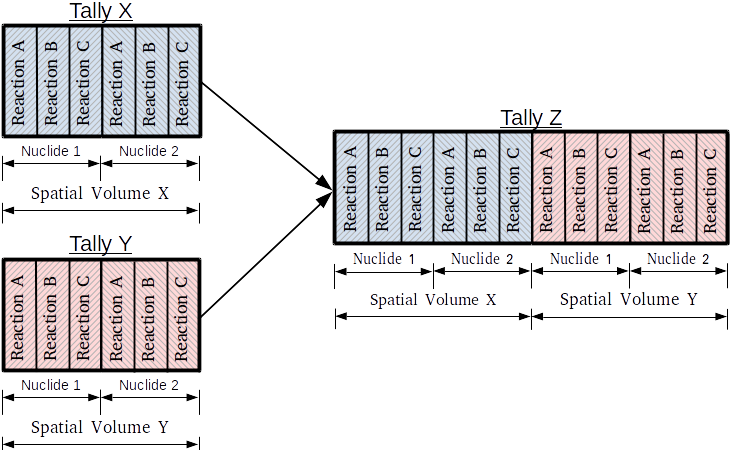
\includegraphics[width=\linewidth]{figures/workflow/openmc/tally-merge}
  \caption{}
\end{subfigure}
\begin{subfigure}{\textwidth}
  \centering
  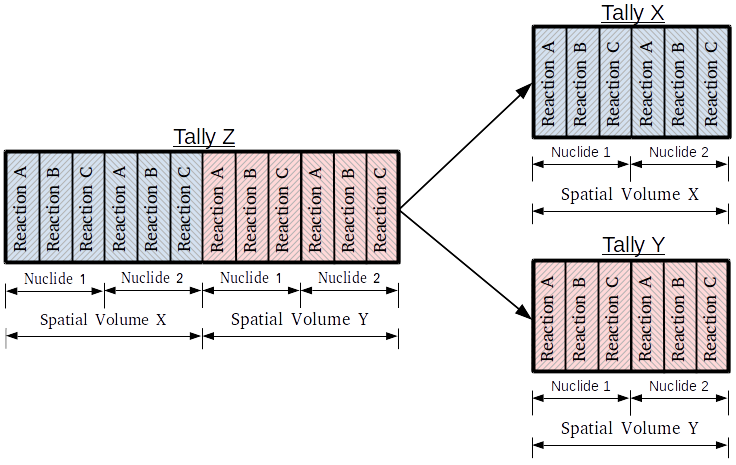
\includegraphics[width=\linewidth]{figures/workflow/openmc/tally-slice}
  \caption{}
\end{subfigure}
\caption[Tally merging and slicing operations]{Two \texttt{Tally} objects for different spatial volumes are merged into a single \texttt{Tally} (a). A single \texttt{Tally} is sliced by spatial volume into two distinct \texttt{Tally} objects (b).}
\label{fig:tally-merge-slice}
\end{figure}

%paragraph: aggregation (slicing/merging)
%-operations use NumPy to efficiently create derived sliced/merged tallies
%-slicing/merging can be used to slice tallies apart by nuclide, group, domain, etc.
%  -use tally merging to re-assembly MGXS from outputs of ML algorithms

%%%%%%%%%%%%%%%%%%%%%%%%%%%%%%%%
\subsubsection{Tally Arithmetic}
\label{subsubsec:chap4-tally-arithmetic}

As discussed in Sec.~\ref{subsec:chap3-tally-types}, a variety of reaction rate and flux tallies must be arithmetically combined in order to compute \ac{MGXS} with Monte Carlo (see Sec.~\ref{subsec:chap3-tally-types}). At the most general level, a reaction rate tally must be divided by a flux tally for each energy group, nuclide and tally volume (see Eqn.~\ref{eqn:chap3-general-micro}). In addition, the transport correction must be subtracted from the total cross section and scattering matrix (Eqns.~\ref{eqn:chap3-sigt-transport-macro} and~\ref{eqn:chap3-scatter-trans-macro}), and a summation must be performed over energy groups to compute the fission emission spectrum (Eqn.~\ref{eqn:chap3-chi}). Furthermore, it is desirable to compute a variance estimator for each \ac{MGXS} by propagating uncertainties as described in Sec.~\ref{subsec:chap3-uncertainty-prop}. The Python \ac{API} provides a novel feature known as \textit{tally arithmetic} to enable arithmetic combinations of tallies with efficient vectorized numerical operations across energy groups, nuclides and spatial tally zones.

Tally arithmetic is an object-oriented data processing feature which arithmetically combines two or more tallies and/or scalar values into new \textit{derived tallies}. The objective of tally arithmetic is to rapidly transform tally data with automated uncertainty propagation. The tally arithmetic implementation in OpenMC overloads the operators for addition, subtraction, multiplication, division, and exponentiation in the Python \ac{API}'s \texttt{Tally} class. In addition, the \texttt{Tally} class supports summation or averaging operations across some or all of its filter, nuclide or score bins.  The derived tallies produced from tally arithmetic provide the same rich functionality available for the \texttt{Tally} operands used in the arithmetic operation (\textit{e.g.}, Pandas DataFrames, tally arithmetic).

Multi-group cross sections may be simply and efficiently computed with tally arithmetic. For example, the following code snippet illustrates how tally slicing and arithmetic are used to compute a total \ac{MGXS}:

\lstinputlisting[language=Python, basicstyle=\ttfamily\scriptsize, caption={\ac{MGXS} calculation with tally arithmetic.}, label={lst:python-input}]{listings/workflow/tally-arithmetic.py}

\noindent The total \ac{MGXS} that is returned from the tally division operation is encapsulated within a \texttt{Tally} class. This is the approach used by the \ac{MGXS} generation module created for OpenMC in Sec.~\ref{subsec:chap4-mgxs}.

It should be noted that the uncertainty propagation in tally arithmetic makes the assumption that tallies represent independent random variables (see Sec.~\ref{subsec:chap3-uncertainty-prop}). However, in many if not most cases this assumption is untrue as tallies may be highly correlated. For example, there is a strong correlation between the flux and reaction rate tallies across the same material or cell, but this is not accounted for when these tallies are combined to compute \ac{MGXS} with tally arithmetic. In the future it may be possible to improve this approximation with the inclusion of tally covariance matrices in tally arithmetic.

%%%%%%%%%%%%%%%%%%%%%%%%%%%%%%%%%%%%%
\subsection{Distributed Cell Tallies}
\label{subsec:chap4-distribcells}

Many Monte Carlo codes, including OpenMC, use some variant of combinatorial geometry. because it can represent arbitrary, repeating geometries such as fuel pins and assemblies. However, the \ac{CG} approach is challenged by applications which require tallies in each instance of a repeated cell throughout a reactor geometry, such as the \ac{BEAVRS} benchmark model~\cite{horelik2013beavrs} depicted in Fig.~\ref{fig:beavrs}. The ``brute force'' solution is to instantiate a unique cell for each distinct tally zone. However, this defeats the purpose of using \ac{CG} for its compact representation, and it is not scalable to problems with large tally datasets such as those considered in this thesis.

\begin{figure}[h!]
  \centering
  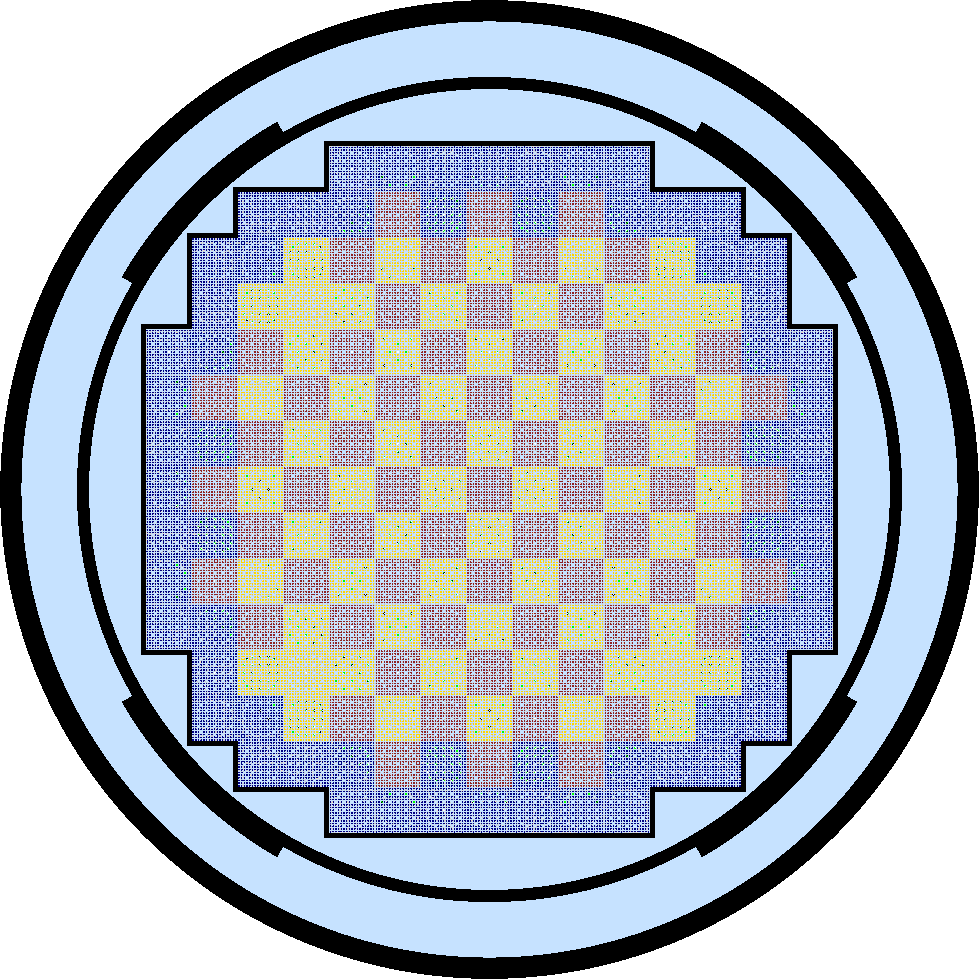
\includegraphics[width=2.5in]{figures/workflow/openmc/core}\hspace{1cm}
  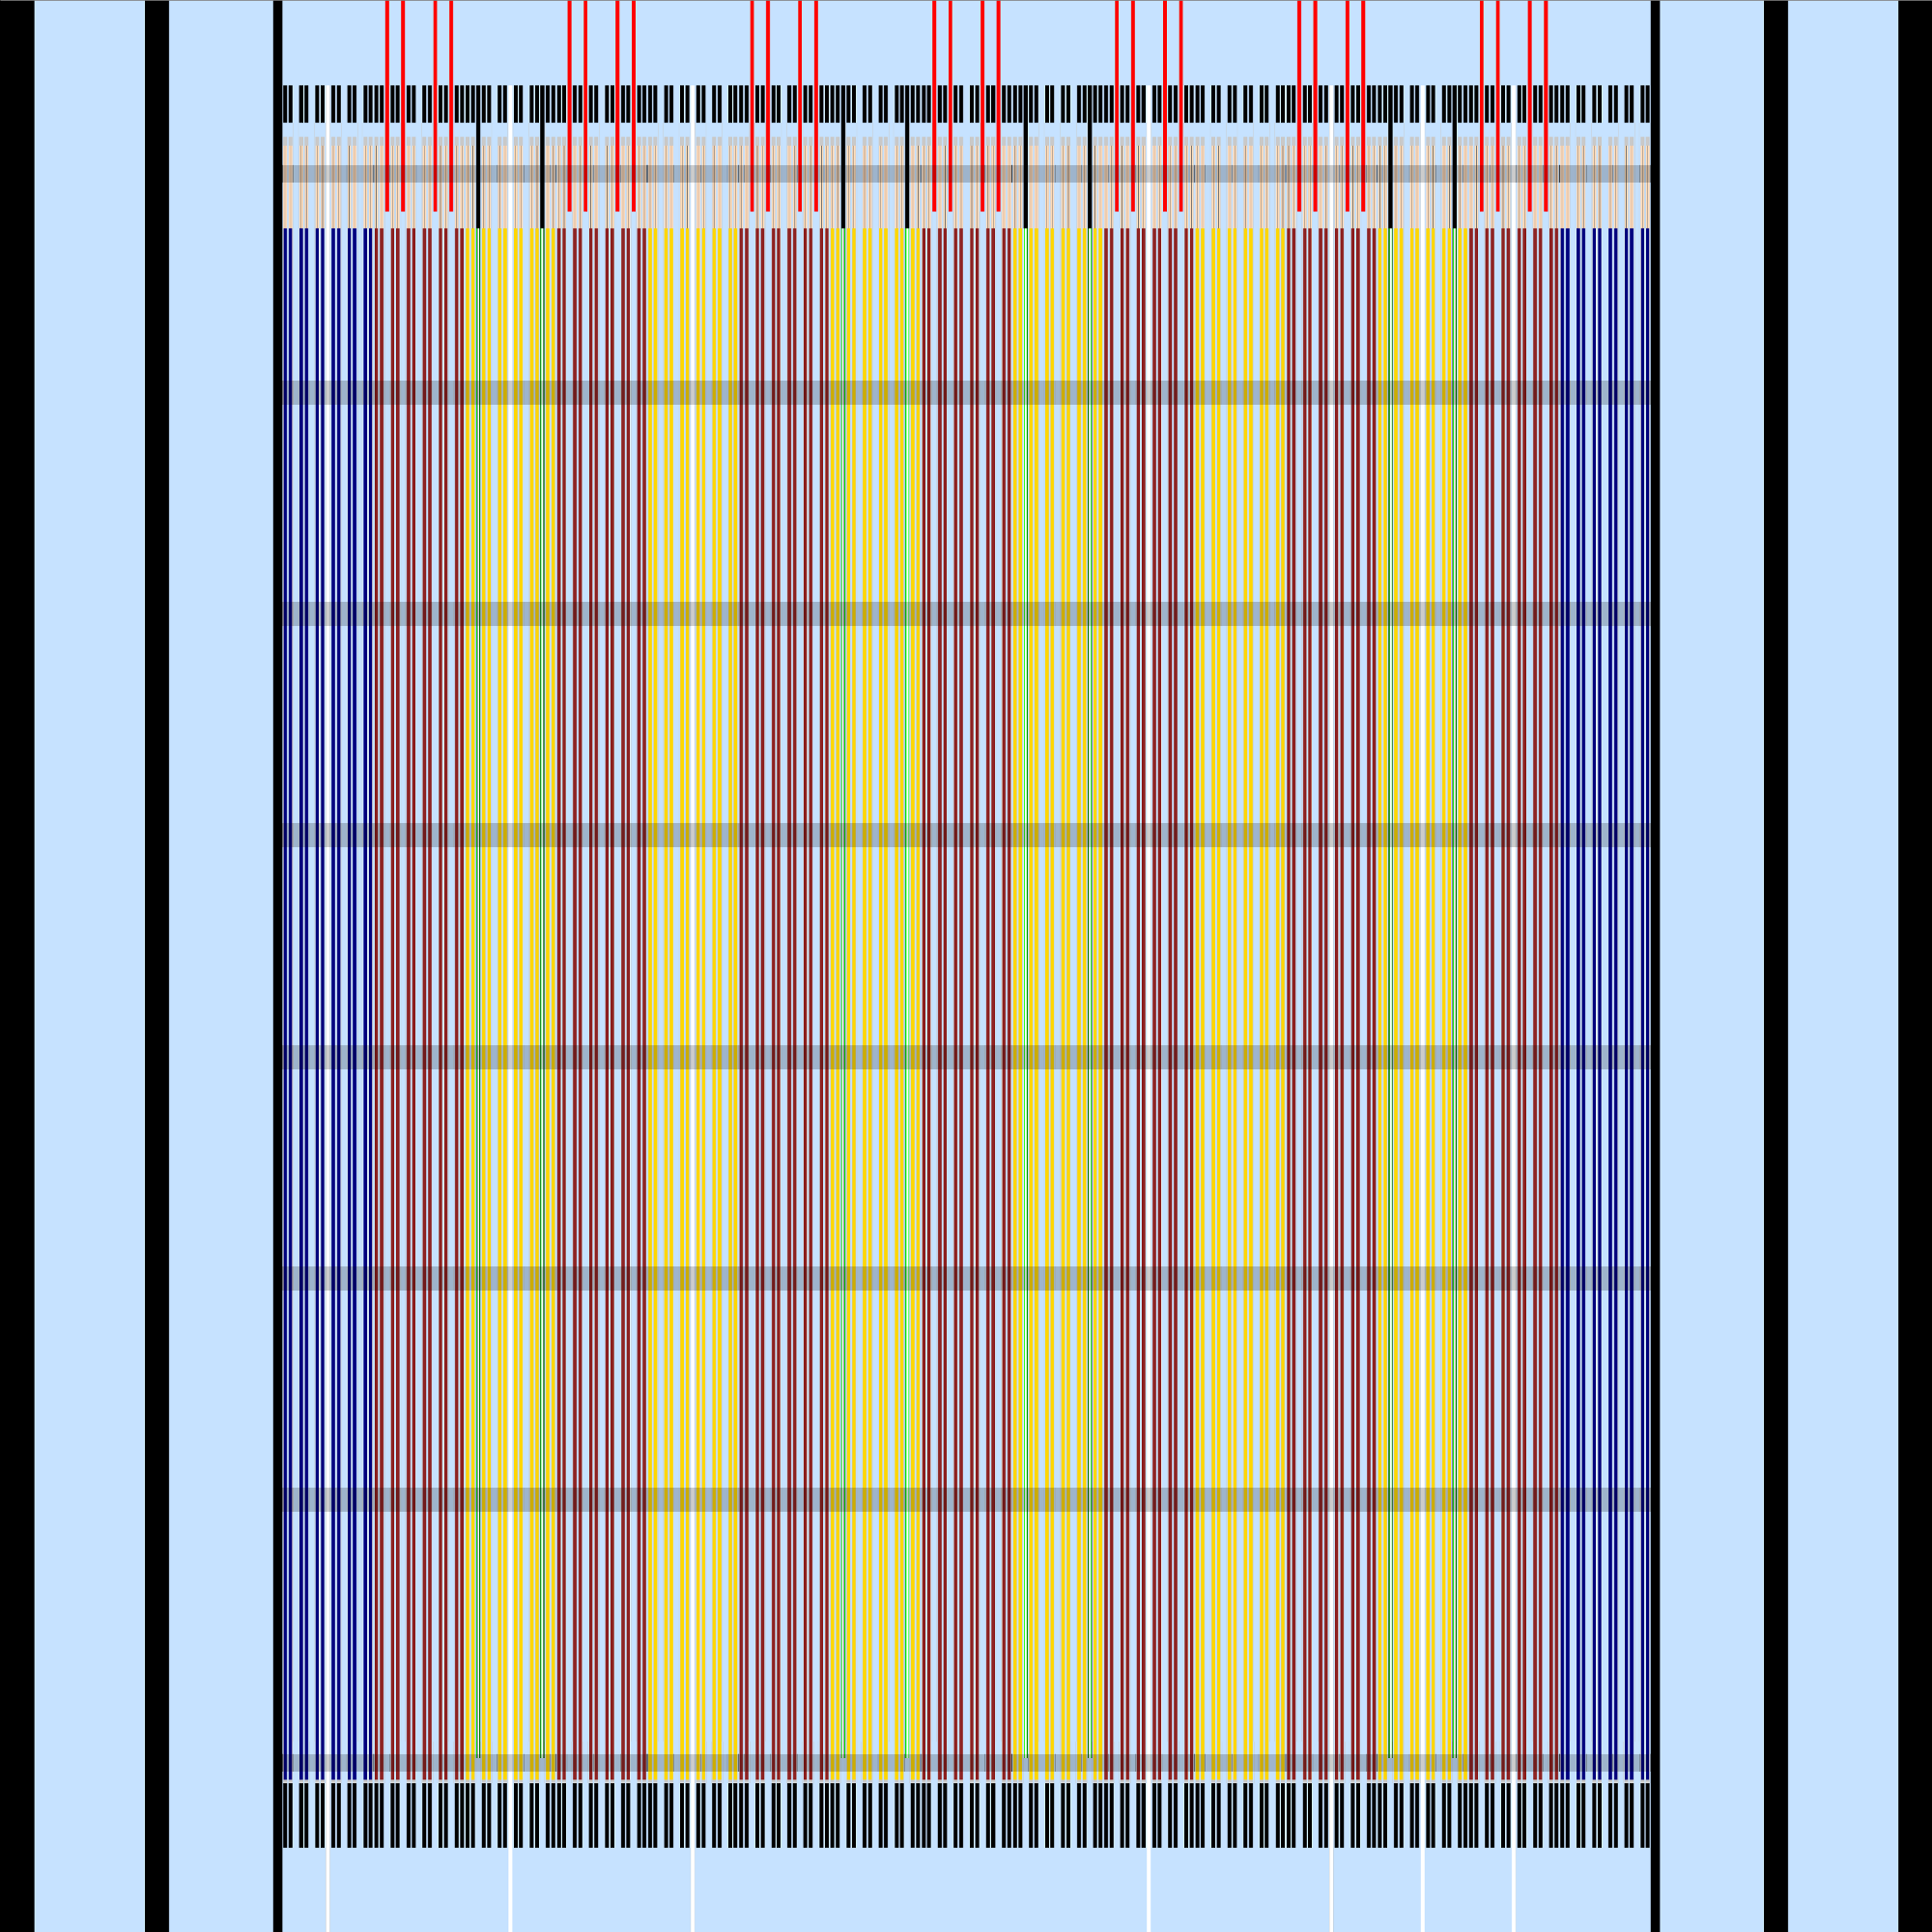
\includegraphics[width=2.5in]{figures/workflow/openmc/core_axial}
\caption[Radial and axial views of the BEAVRS core]{The radial (a) and axial (b) views of the BEAVRS \ac{PWR} core geometry~\cite{horelik2013beavrs}. The distributed cell tally algorithm provides a simple and efficient interface to tally within each of the 50,000+ fuel, guide tube, and burnable poison pin cells in complex heterogeneous models like the \ac{BEAVRS} core.}
\label{fig:beavrs}
\end{figure}

The \textit{distributed cell tally} algorithm was implemented in OpenMC to permit simply defined spatial tally zones across repeated cell instances~\cite{lax2014distribcell}. The distributed cell algorithm, commonly abbreviated as the \textit{distribcell} algorithm, classifies each unique cell instance using \textit{maps} and \textit{offsets} which consume orders of magnitude less memory than would be required by the ``brute force'' approach. Only a single transparent line of \ac{XML} input is necessary to define a distribcell tally which may span across an arbitrary number of instances for a particular cell. Furthermore, the Python \ac{API} may be used to perform efficient vectorized transformations of distribcell tally data stored as contiguous NumPy arrays. The distribcell tally algorithm was used to compute spatially-varying \ac{MGXS} across fuel pin cell instances for the spatial homogenization methology introduced in Chaps.~\Crefrange{chap:benchmarks}{chap:unsupervised}.

The distribcell tally algorithm consists of pre-processing and indexing stages. The pre-processing phase builds a mapping to index unique regions based on the unique combination of cells, universes and lattices used to construct each region. This is done by storing offset numbers in the data structures for each fill cell\footnote{Any cell that is filled with a nested universe or lattice of cells.}. The offset maps are recursively constructed starting from the top-level universe and proceeding through each lower nested universe level in the combinatorial geometry. The pre-processing algorithm tabulates the total number of instances of each cell in the geometry in order to dynamically allocate memory for distribcell tally arrays. At runtime, the on-the-fly indexing scheme efficiently computes cell instance IDs in order to index and score to the appropriate bin(s) in distribcell tallies. The cell instance IDs are simply found by summing the offsets at each nested universe level along the path to the cell instance in the \ac{CG} as shown in Fig.~\ref{fig:indexing-scheme}. The interested reader is referred to~\cite{lax2014distribcell} for details about the distribcell tally algorithm, including pseudocode for pre-processing and indexing and a performance model for the memory footprint consumed by offsets and maps.

\begin{figure}
  \centering
  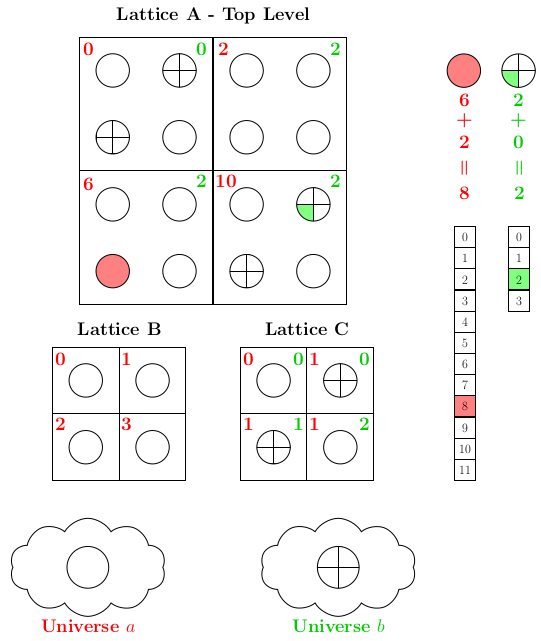
\includegraphics[width=\linewidth]{figures/workflow/openmc/distribcells}
\caption[The distributed cell tally indexing algorithm]{An example of the distribcell tally algorithm's on-the-fly indexing scheme~\cite{lax2014distribcell}. Material-filled cells are defined in pin cell universes $a$ and $b$, which are filled into the cells of lattices $B$ and $C$, which are filled into the cells of lattice $A$.  The colored numbers in each fill cell are the offsets for each base universe, which can be used to quickly compute a unique ID for each instance of a material cell.}
\label{fig:indexing-scheme}
\end{figure}

%%%%%%%%%%%%%%%%%%%%%%%%%%%%%%%%%%%%%%%%
\subsection{Isotropic in Lab Scattering}
\label{subsec:chap4-iso-in-lab}

As part of this thesis, a unique option for isotropic in lab scattering was implemented in the OpenMC code. The isotropic in lab (abbreviated as iso-in-lab) feature may be useful to quantify the ability of multi-group codes to capture anisotropic scattering effects with higher order scattering matrices or transport correction schemes (see Sec.~\ref{subsec:chap2-transport-corr}). The iso-in-lab scattering feature was implemented as a ``scattering'' attribute for each nuclide/element in a simulation. When iso-in-lab scattering is specified for a nuclide/element, the outgoing neutron energy is sampled from the scattering laws prescribed by the continuous energy cross section library, but the outgoing neutron direction of motion is sampled from an isotropic in lab distribution. 

Unless otherwise noted, isotropic in lab scattering was employed in OpenMC to generate the \ac{MGXS} used in this thesis. The iso-in-lab scattering feature enabled ``apples-to-apples'' comparisons between the reference eigenvalues and reaction rates produced by OpenMC and those computed from isotropic multi-group calculations with OpenMOC.

%%%%%%%%%%%%%%%%%%%%%%%%%%%%
\subsection{MGXS Generation}
\label{subsec:chap4-mgxs}

The OpenMC Python \ac{API}'s \texttt{openmc.mgxs} module was implemented to generate multi-group cross sections. The \texttt{openmc.mgxs} module is built atop the underlying core features in the rest of the \ac{API} to support a seamless interface for both input generation and downstream data processing of \ac{MGXS} from Python. In particular, one may specify the \ac{MGXS} to compute and the \texttt{openmc.mgxs} module will construct the necessary \texttt{Tally} objects. The \texttt{Tally} objects may be easily exported to \ac{XML} input files for OpenMC, and used to containerize and process the tally data produced by an OpenMC simulation. The \texttt{openmc.mgxs} module thereby leverages the software stack of Pandas DataFrames, tally arithmetic, etc. provided by the OpenMC Python \ac{API}.

The \texttt{openmc.mgxs} module can compute macroscopic or microscopic \ac{MGXS} for individual nuclides or elements as well as collections of nuclides and elements\footnote{A \ac{MGXS} computed for a collection of nuclides/elements is the sum of the individual contributions from each nuclide/element.}. \ac{MGXS} can be computed in one or more arbitrary energy group structures. The module supports energy condensation in downstream data processing which is useful for exploring approximation bias in various energy group structures. For example, \ac{MGXS} may be computed in a 16-group structure and the tally data subsequently condensed to 2-group, 8-group, 12-group, etc. structures for multi-group calculations\footnote{Energy condensation may be performed to arbitrarily defined coarse group structures with \texttt{openmc.mgxs} provided the coarse group boundaries coincide with boundaries in the fine group structure.}. The analysis in this thesis computed \ac{MGXS} in the 70-group structure provided in Tab.~\ref{table:app-70-groups}, and condensed the \ac{MGXS} to the coarser group structures given in Appendix~\ref{app:energy-groups} as needed.

The \texttt{openmc.mgxs} module is designed to perform spatial homogenization on heterogeneous tally meshes for fine mesh transport codes. In OpenMC parlance, \ac{MGXS} may be computed for material, cell or universe spatial domains. In addition, the module supports \ac{MGXS} calculations for repeated cell instances using distribcell spatial tally domains (see Sec.~\ref{subsec:chap4-distribcells}). The \texttt{openmc.mgxs} module may also perform spatial homogenization on structured Cartesian tally meshes for coarse mesh multi-gropu calculations. This thesis computed \ac{MGXS} using distribcell tallies (\textit{e.g.}, \ac{MGXS} for each fuel pin instance in a geometry) to support the \ac{MGXS} spatial homogenization introduced in Chaps.~\Crefrange{chap:benchmarks}{chap:unsupervised}.

The \texttt{openmc.mgxs} module uses an object-oriented design based on an abstract \texttt{MGXS} class with subclasses for different reaction types. The \texttt{MGXS} subclasses are itemized in Tab.~\ref{table:chap4-mgxs-types} and compute multi-group constants from \ac{MC} tallies using the methods detailed in Sec.~\ref{subsec:chap3-tally-types}. It should be noted that some reaction types include variants which do or do not account for scattering multiplicity reactions (see Sec.~\ref{sec:chap2-scatt-prod}). For example, the transport correction used by the \texttt{TransportXS} class does not include $(n,xn)$ reactions while that employed by the \texttt{NuTransportXS} does account for scattering multiplicity. The \texttt{openmc.mgxs} module also includes a \texttt{Library} class which automates the construction of \texttt{MGXS} objects for different group structures, spatial domains, and reaction types.

\begin{table}[h!]
  \centering
  \caption[The MGXS types implemented for OpenMC]{The \ac{MGXS} types implemented by the \texttt{openmc.mgxs} module in OpenMC.}
  \small
  \label{table:chap4-mgxs-types} 
  \vspace{6pt}
  \begin{tabular}{l p{10cm}}
  \toprule
  \rowcolor{lightgray}
  {\bf Class} &
  {\bf Description} \\
  \midrule
  \texttt{TotalXS} & Total collision \\
  \texttt{TransportXS} & Transport-corrected total collision \\
  \texttt{NuTransportXS} & Transport-corrected total collision w/ scattering multiplicity \\
  \texttt{AbsorptionXS} & Absorption \\
  \texttt{CaptureXS} & Radiative capture \\
  \texttt{FissionXS} & Fission \\
  \texttt{NuFissionXS} & Fission production \\
  \texttt{KappaFissionXS} & Fission energy release \\
  \texttt{ScatterXS} & Scattering \\
  \texttt{NuScatterXS} & Scattering w/ scattering multiplicity \\
  \texttt{ScatterMatrixXS} & Scattering matrix \\
  \texttt{NuScatterMatrixXS} & Scattering matrix w/ scattering multiplicity \\
  \texttt{Chi} & Fission emission spectrum \\
  \texttt{ChiPrompt} & Prompt fission emission spectrum \\
  \bottomrule
\end{tabular}
\end{table}

The \texttt{openmc.mgxs} module was developed with general design principles to generate \ac{MGXS} for any multi-group neutron transport code. Although the module does not explicitly support any multi-group codes, it can export \ac{MGXS} data to a variety of data storage formats, including \ac{CSV} and \ac{HDF5}. The exported \ac{MGXS} files may be easily transformed into the database or input files required by a particular multi-group code. As discussed in the following section, this thesis developed a tightly integrated framework to pipeline \ac{MGXS} generated by \texttt{openmc.mgxs} into the multi-group OpenMOC code.

\begin{emphbox}
\textbf{The OpenMC code was used to generate \ac{MGXS}. A Python \ac{API} was implemented for input generation and data processing, along with features including distributed cell tallies and isotropic in lab scattering. The \texttt{openmc.mgxs} Python module was created to generate \ac{MGXS} from OpenMC tallies.}
\end{emphbox}


%%%%%%%%%%%%%%%%%%%%%%%%%%%%%%%%%%%%%%%%%%%%%%%%%%%%%%%%%%%%%%%%%%%%%%%%%%%%%%%%
\section{OpenMOC}
\label{sec:chap4-openmoc}

The OpenMOC code is a multi-group neutron transport code implementing the deterministic Method of Characteristics (MOC)~\cite{boyd2014openmoc}. OpenMOC was initially developed to support a series of M.S. theses at MIT~\cite{li2013ms,boyd2014ms,shaner2014ms} and was later released for public use with the MIT open source license. Although this thesis could have plausibly used any multi-group code, OpenMOC was chosen for its flexible Python interface, computationally efficient algorithms, and the author's familiarity with the open source codebase.

%-reference need for MG code to evaluate MGXS for this thesis

This thesis inspired the development of new features and extensions which have been incorporated into the official OpenMOC codebase. This section begins with a brief overview of the \ac{MOC} implementation in OpenMOC in Sec.~\ref{subsubsec:chap4-openmoc-overview}. Various improvements were made to the OpenMOC Python interface as discussed in Sec.~\ref{subsubsec:chap4-openmoc-python}, while Sec.~\ref{subsubsec:chap4-openmoc-mgxs} details a module created to interface with \ac{MGXS} generated by OpenMC. The parallel algorithms and numerical acceleration schemes in OpenMOC which were used by this thesis are mentioned in Secs.~\ref{subsubsec:chap4-openmoc-parallel} and~\ref{subsubsec:chap4-openmoc-cmfd}, respectively.

%-improvements to the parallelism, CMFD to enable ``multi-sim'' calculations

%%%%%%%%%%%%%%%%%%%%%%%%%%%%%%%%%
\subsection{Methods Overview}
\label{subsubsec:chap4-openmoc-overview}

The method of characteristics is a widely used technique for solving partial differential equations, including the Boltzmann form of the neutron transport equation~\cite{askew1972moc}. Although not a stochastic formulation, \ac{MOC} is a ray-based algorithm akin to Monte Carlo particle tracking-based methods. In contrast to Monte Carlo, \ac{MOC} uses a fixed angular quadrature that is determined \textit{a priori}. This quadrature is used to specify 1D characteristics that cross the spatial domain. Prior to the physics computation, ray tracing must be performed to subdivide each characteristic into segments within different regions in the spatial mesh. Fig.~\ref{fig:moc-model} illustrates the spatial mesh and cyclic characteristic laydown used by the OpenMOC code.

\ac{MOC} propagates the angular neutron flux along each characteristic through each spatial zone. For each segment, the angular flux is attenuated due to neutron absorption and enhanced due to neutron fission or scattering in the corresponding spatial zone. \ac{MOC} uses the multi-group energy approximation such that this computation is performed for neutrons within discretized energy groups (see Sec.~\ref{subsec:chap2-energy}). Finally, an angular quadrature is applied to combine the average angular flux contribution from each characteristic to compute the average scalar flux in each zone and energy group.

\begin{figure}[h!]
  \begin{subfigure}[htb!]{0.32\textwidth}
    \centering
    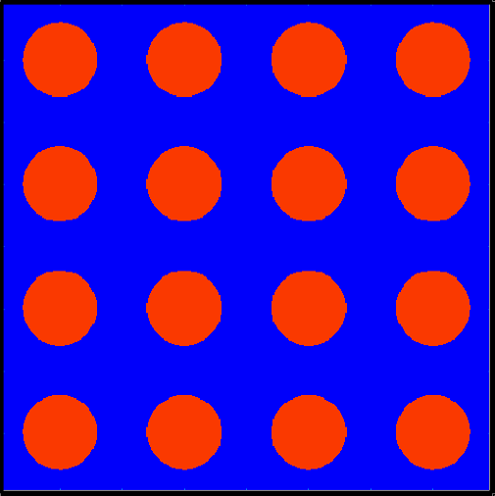
\includegraphics[width=0.95\textwidth]{figures/workflow/openmoc/materials-border}
    \label{fig:moc-model-materials}
    \caption{}
  \end{subfigure}
  \begin{subfigure}[htb!]{0.32\textwidth}
    \centering
    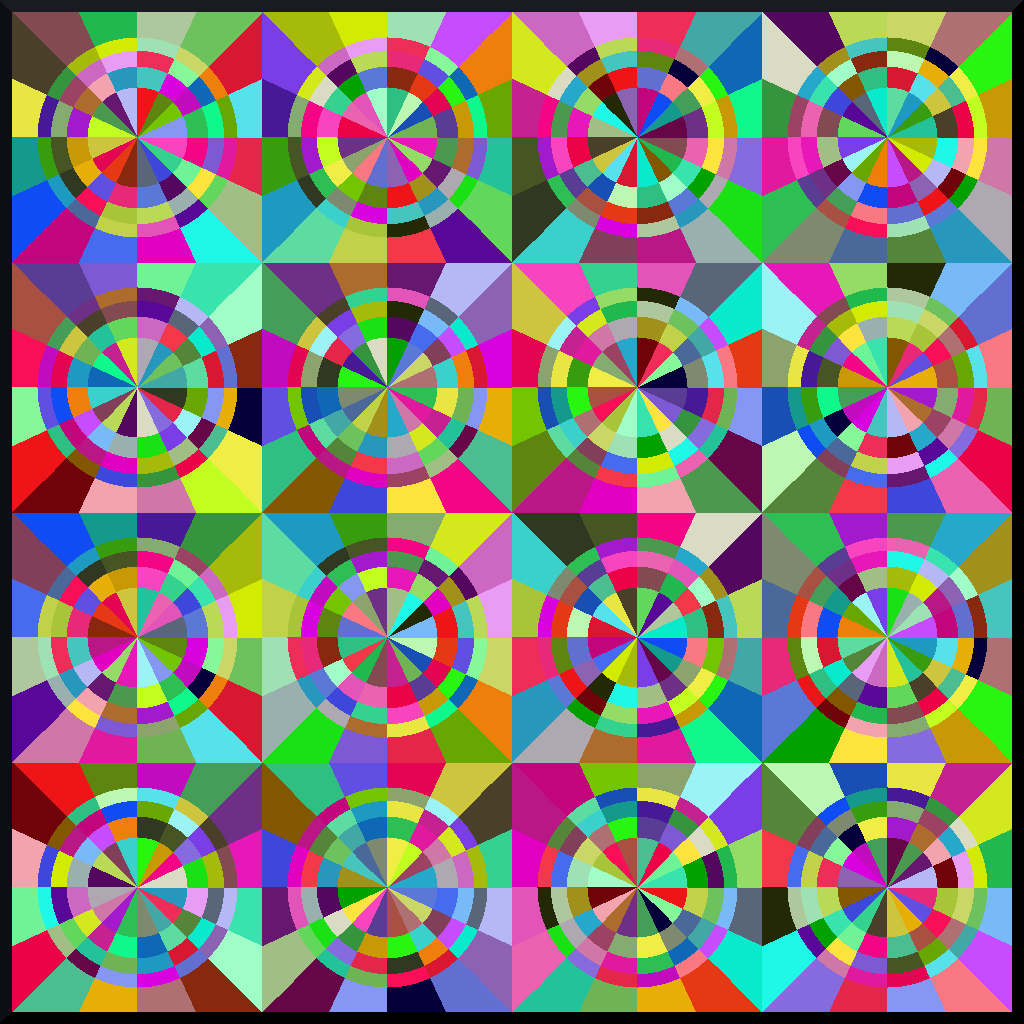
\includegraphics[width=0.95\textwidth]{figures/workflow/openmoc/FSRs}
    \label{fig:moc-model-fsrs}
    \caption{}
  \end{subfigure}
  \begin{subfigure}[htb!]{0.32\textwidth}
    \centering
    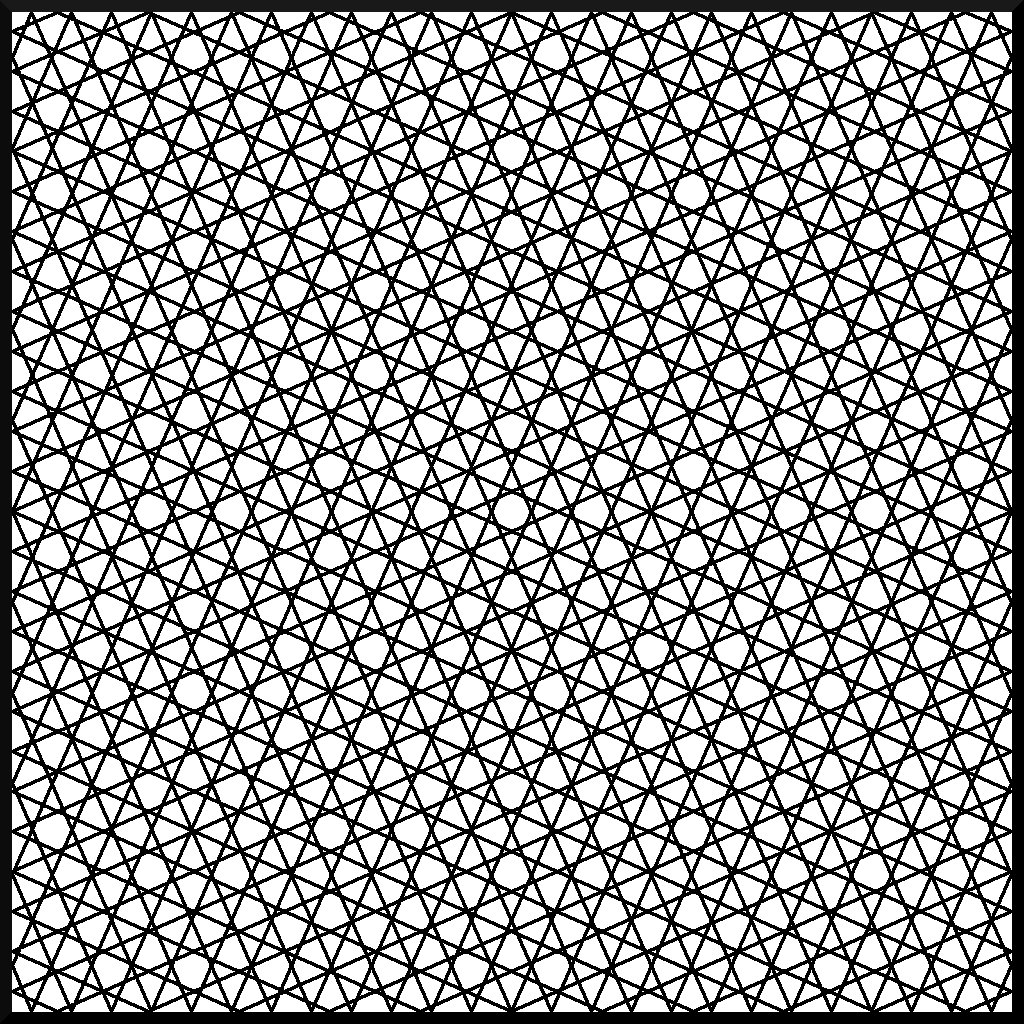
\includegraphics[width=0.95\textwidth]{figures/workflow/openmoc/cyclic-tracks}
    \label{fig:moc-model-tracks}
    \caption{}
  \end{subfigure}
\caption[Example OpenMOC flat source region mesh and track laydown]{The coolant and fuel materials (a), flat source region spatial mesh (b), and cyclic characteristic laydown (c) for a 4 $\times$ 4 fuel pin lattice taken from~\cite{boyd2016parallel}.}
\label{fig:moc-model}
\end{figure}

The OpenMOC code is capable of performing 2D \ac{MOC} calculations for light water reactor core configurations. OpenMOC discretizes the 2D geometry into flat source regions (FSRs) which approximate the neutron source as constant across each spatial zone\footnote{The neutron source may include any combination of fission, scattering and fixed sources.}. Furthermore, OpenMOC approximates the scattering source as isotropic in the lab coordinate system and is not yet able to use higher order scattering moment matrices. OpenMOC uses a power iteration scheme to solve for the dominant eigenvalue and eigenvector in criticality calculations. As part of this thesis, a general purpose fixed source solver was implemented to enable the detailed investigation of approximation bias in \ac{MGXS} as discussed in Chap.~\ref{chap:sph}. The interested reader is referred to the online code manual~\cite{openmoc2016manual} for more information detailing the \ac{MOC} implementation in OpenMOC.

%%%%%%%%%%%%%%%%%%%%%%%%%%%%%%%%%
\subsection{Python Interface}
\label{subsubsec:chap4-openmoc-python}

One of the key reasons that OpenMOC was used by this thesis was to leverage its flexible Python interface. The majority of the source code is written in C++ using object-oriented software design principles. The \ac{SWIG}~\cite{beazley2003swig} is deployed to expose the C++ classes and routines to the Python scripting language. The Python interface made it possible to tightly couple OpenMOC with the rich ecosystem of Python-based data processing and visualization tools for the spatial homogenization methodology developed in Chaps.~\Crefrange{chap:benchmarks}{chap:unsupervised}.

As part of this work, a new scheme was implemented to efficiently link OpenMOC's Python and C++ \ac{CG} data structures into a hierarchical tree-like data structure. This made it possible to use the OpenCG region differentiation algorithm discussed in Sec.~\ref{sec:chap4-region-diff} to derive geometries for OpenMOC. In addition, a thread-safe memory management model was realized which unifies the dynamic deallocation of objects shared between Python and C++ code. The memory model enabled 100s of OpenMOC simulations to be orchestrated by Python for the parametric studies considered in this thesis.

%\begin{figure}[h!]
%  \centering
%  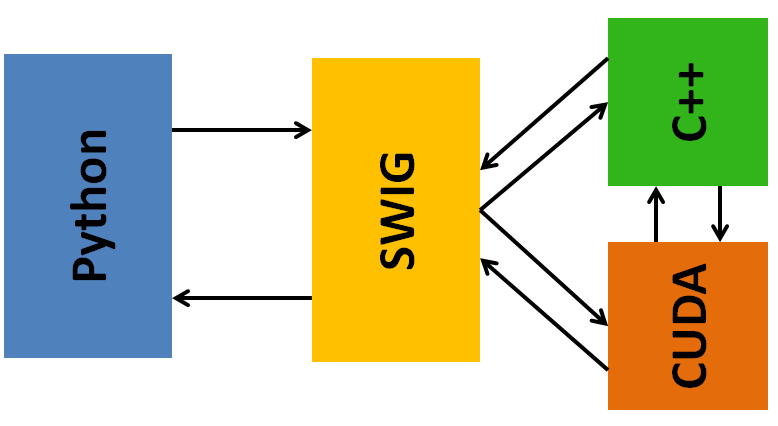
\includegraphics[width=0.7\linewidth]{figures/workflow/openmoc/software-design}
%\caption[The OpenMOC programming model]{The programming model used by OpenMOC to couple compiled C/C++/CUDA code to the Python interface using \ac{SWIG} taken from~\cite{boyd2014openmoc}.}
%\label{fig:openmoc-swig}
%\end{figure}

%%%%%%%%%%%%%%%%%%%%%%%%%%%%%%%%%
\subsection{Multi-Group Cross Sections}
\label{subsubsec:chap4-openmoc-mgxs}

OpenMOC uses multi-group macroscopic nuclear cross sections specified in any arbitrary energy group structure. Isotropic concentrations are not used since OpenMOC does not perform self-shielding or depletion calculations. Multi-group cross sections may be specified for each material or cell in the \ac{CG} used in a simulation. OpenMOC requires total, fission production and scattering matrix cross sections along with a fission emission spectrum\footnote{Transport-corrected total cross sections and scattering matrices may be used in OpenMOC.}. In addition, a fission cross section may be optionally supplied in order to compute spatially-varying fission reaction rates.

Cross section data is encapsulated by the \texttt{Material} class. A \texttt{Material} object may be instantiated in Python and cross section data loaded into it from NumPy arrays~\cite{walt2011numpy}. For simulations with many different materials (such as those in this thesis), defining nuclear cross section data by hand in a Python script is cumbersome and error prone. In order to minimize this painstaking process, the \texttt{openmoc.materialize} module was implemented to automate the loading \ac{MGXS} data into OpenMOC \texttt{Material} objects. This module can either import \ac{MGXS} data from HDF5 binary files~\cite{koranne2011hdf5} or extract \ac{MGXS} data from OpenMC \texttt{Library} Python objects (see Sec.~\ref{subsec:chap4-mgxs}). The \texttt{openmoc.materialize} module is designed to support large \ac{MGXS} libraries such as those produced from the spatial homogenization methodology introduced in Chaps.~\Crefrange{chap:benchmarks}{chap:unsupervised}. In addition, a scheme to compute \ac{SPH} factors to ensure reaction rate consistency with OpenMC was implemented in \texttt{openmoc.materialize} and is discussed in detail in Chap.~\ref{chap:sph}.

%%%%%%%%%%%%%%%%%%%%%%%%%%%%%%%%%
\subsection{Parallelism}
\label{subsubsec:chap4-openmoc-parallel}

OpenMOC's high performance parallel solvers for both multi-core \ac{CPUs} and \ac{GPUs} were extensively used for the analyses presented in this thesis. A shared memory parallel solver implemented in C++ using OpenMP~\cite{openmp2013} has demonstrated excellent scalability on a range of multi-core architectures\cite{boyd2016parallel}. In addition, OpenMOC includes a highly parallel implementation which uses the CUDA programming language~\cite{nvidia2012cuda} to run on NVIDIA \ac{GPUs} with 100s to 1000s of lightweight cores~\cite{boyd2013massively}. OpenMOC's parallel solvers made it possible to perform large parametric studies of 100s of \ac{MOC} simulations to evaluate the spatial homogenization methodology introduced in Chaps.~\Crefrange{chap:benchmarks}{chap:unsupervised}.


%%%%%%%%%%%%%%%%%%%%%%%%%%%%%%%%%
\subsection{CMFD Acecleration}
\label{subsubsec:chap4-openmoc-cmfd}

OpenMOC uses the Coarse Mesh Finite Difference (CMFD) acceleration scheme to greatly reduce the number of iterations required to converge criticality calculations~\cite{boyd2014openmoc}. \ac{CMFD} acceleration functions by using the solution of a coarse mesh diffusion problem to accelerate the convergence of the fine mesh \ac{MOC} transport problem. The details of the \ac{CMFD} implementation in OpenMOC are beyond the scope of this thesis, and the interested reader is referred to the online code manual~\cite{openmoc2016manual} for more information. 

\ac{CMFD} acceleration was extensively used to accelerate the eigenvalue calculations in this thesis. All simulations which employed \ac{CMFD} used the novel $k$-Nearest Neighbors prolongation scheme created by Shaner~\cite{shaner2015cmfd} and implemented in OpenMOC to improve the convergence rate and stability of \ac{CMFD}. In particular, all simulations used three neighbors along with a successive over-relaxation (SOR) factor of unity. Along with OpenMOC's parallel solvers, \ac{CMFD} acceleration made it feasible to perform large parametric studies to generate the results presented in this thesis.

%\begin{figure}[h!]
%  \centering
%  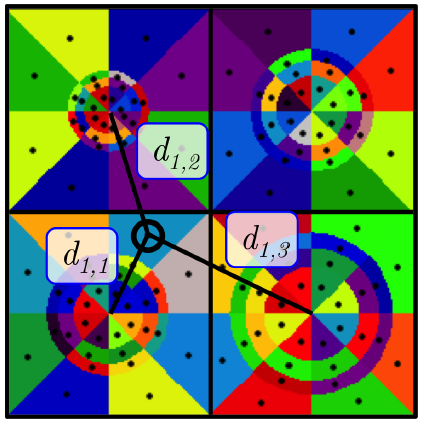
\includegraphics[width=0.5\linewidth]{figures/workflow/openmoc/centroid}
%\caption[$k$-nearest neighbor centroid scheme for CMFD]{The $k$-nearest neighbor centroid update scheme for \ac{CMFD}~\cite{shaner2015cmfd}.}
%\label{fig:knn-cmfd}
%\end{figure}

\begin{emphbox}
\textbf{The OpenMOC code was used to perform 2D deterministic multi-group \ac{MOC} calculations. The \texttt{openmoc.materialize} module was improved to support \ac{MGXS} generated from OpenMC. OpenMOC's parallel algorithms and \ac{CMFD} acceleration enabled parametric studies of 100s of OpenMOC simulations.}
\end{emphbox}


%%%%%%%%%%%%%%%%%%%%%%%%%%%%%%%%%%%%%%%%%%%%%%%%%%%%%%%%%%%%%%%%%%%%%%%%%%%%%%%%
\section{OpenCG}
\label{sec:chap4-opencg}

The OpenCG code~\cite{boyd2015opencg} was created to simplify the process of creating and transferring data mapped to combinatorial geometries for OpenMC and OpenMOC. Combinatorial geometry\footnote{\ac{CG} is often referred to as constructive solid geometry in the neutron transport literature.} is commonly used by neutron transport simulation codes since it:

\begin{itemize}[noitemsep]
  \item Permits description of an \textit{arbitrarily accurate} unstructured geometric mesh
  \item Provides a \textit{compact representation} with minimal input description
  \item Represents $\mathcal{O}(n)$ components with $\mathcal{O}(\log{}n)$ memory requirements
  \item Utilizes a hierarchical \textit{tree data structure} with scalable $\mathcal{O}(\log{}n)$ traversals
\end{itemize}

\noindent Although many codes utilize \ac{CG}, it is overly burdensome to manually write geometric input files for multiple simulation tools for code verification of a single reactor model. In addition, the compact geometric representation is not well-suited for large scale analysis of spatially-varying data in nuclear reactor cores -- such as distributed cell tally data in OpenMC -- without new algorithms to guide and automate the process. This thesis developed a new \ac{CG} modeling tool called OpenCG to accelerate the building of complicated reactor geometries, enable rapid cross-code verification and facilitate large scale data processing. 

OpenCG is a simple-to-use Python library which may be used to construct a single geometry for use in both OpenMC and OpenMOC. In addition, OpenCG enables data transfer between OpenMC and OpenMOC as illustrated in Fig.~\ref{fig:chap4-simulation-triad}. In particular, OpenCG accomodates the generation of \ac{MGXS} from distributed cell tallies on OpenMC's \ac{CG} mesh and maps them to the flat source region spatial mesh used by OpenMOC. A variant of OpenMC's distributed cell tally algorithm (see Sec.~\ref{subsec:chap4-distribcells}) was implemented in OpenCG to make this possible. In addition to transferring \ac{MGXS} data, OpenCG enabled the comparison of pin-wise reaction rate distributions computed from OpenMC distribcell tallies with those computed on OpenMOC's \ac{FSR} mesh.

The following sections outline the key features implemented in OpenCG for this thesis and follows a recent paper by this author~\cite{boyd2015opencg}. Sec.~\ref{sec:chap4-opencg-compatibility} discusses the compatibility modules which tie OpenCG, OpenMC and OpenMOC into a simulation triad. In addition, two novel algorithms known as \ac{LNS} and region differentiation were developed in OpenCG to enable the spatial homogenization methodology introduced in this thesis, and are presented in Secs.~\ref{sec:chap4-lns} and~\ref{sec:chap4-region-diff}, respectively.

%%%%%%%%%%%%%%%%%%%%%%%%%%%%%%%%%%%%
\subsection{Compatiblity Modules}
\label{sec:chap4-opencg-compatibility}

The simulation triad of OpenCG, OpenMC and OpenMOC shown in Fig.~\ref{fig:chap4-simulation-triad} is made possible with compatibility modules. The compatibility modules allow the construction of a single geometry using OpenCG's Python \ac{CG} primitives for surfaces, cells, universes and lattices. The OpenCG geometry may then be exported to OpenMC or OpenMOC using compatibility modules developed for each code.

For example, OpenMC includes a Python \ac{API} with object-oriented \ac{CG} primitives. This \ac{API}'s primitives include routines to directly export themselves to the \ac{XML} input file format used by OpenMC. The OpenCG-OpenMC compatibility module allows OpenCG's primitives to be transformed into the corollaries within the OpenMC Python \ac{API}, and vice versa. Likewise, the OpenCG-OpenMOC compatibility module allows OpenCG's primitives to be transformed into the corollaries within the OpenMOC Python/C++ code. In summary, the compatibility modules enable the rapid, automated exportation of various OpenCG geometries directly to OpenMC and OpenMOC.

OpenCG's object-oriented Python software model permits greater freedom for geometric parameter optimization than can be easily achieved with traditional \ac{ASCII} or \ac{XML} input files. In particular, the compatibility module framework enabled a dynamic workflow between OpenMC and OpenMOC for \ac{MGXS} generation and code verification in this thesis. For example, OpenCG's region differentiation algorithm (see Sec.~\ref{sec:chap4-region-diff}) was used to produce 100s of geometries composed with different \ac{MGXS} libraries to evaluate the spatial homogenization methodology introduced in Chaps.~\Crefrange{chap:benchmarks}{chap:unsupervised}.

%\begin{figure}[h!]
%  \centering
%  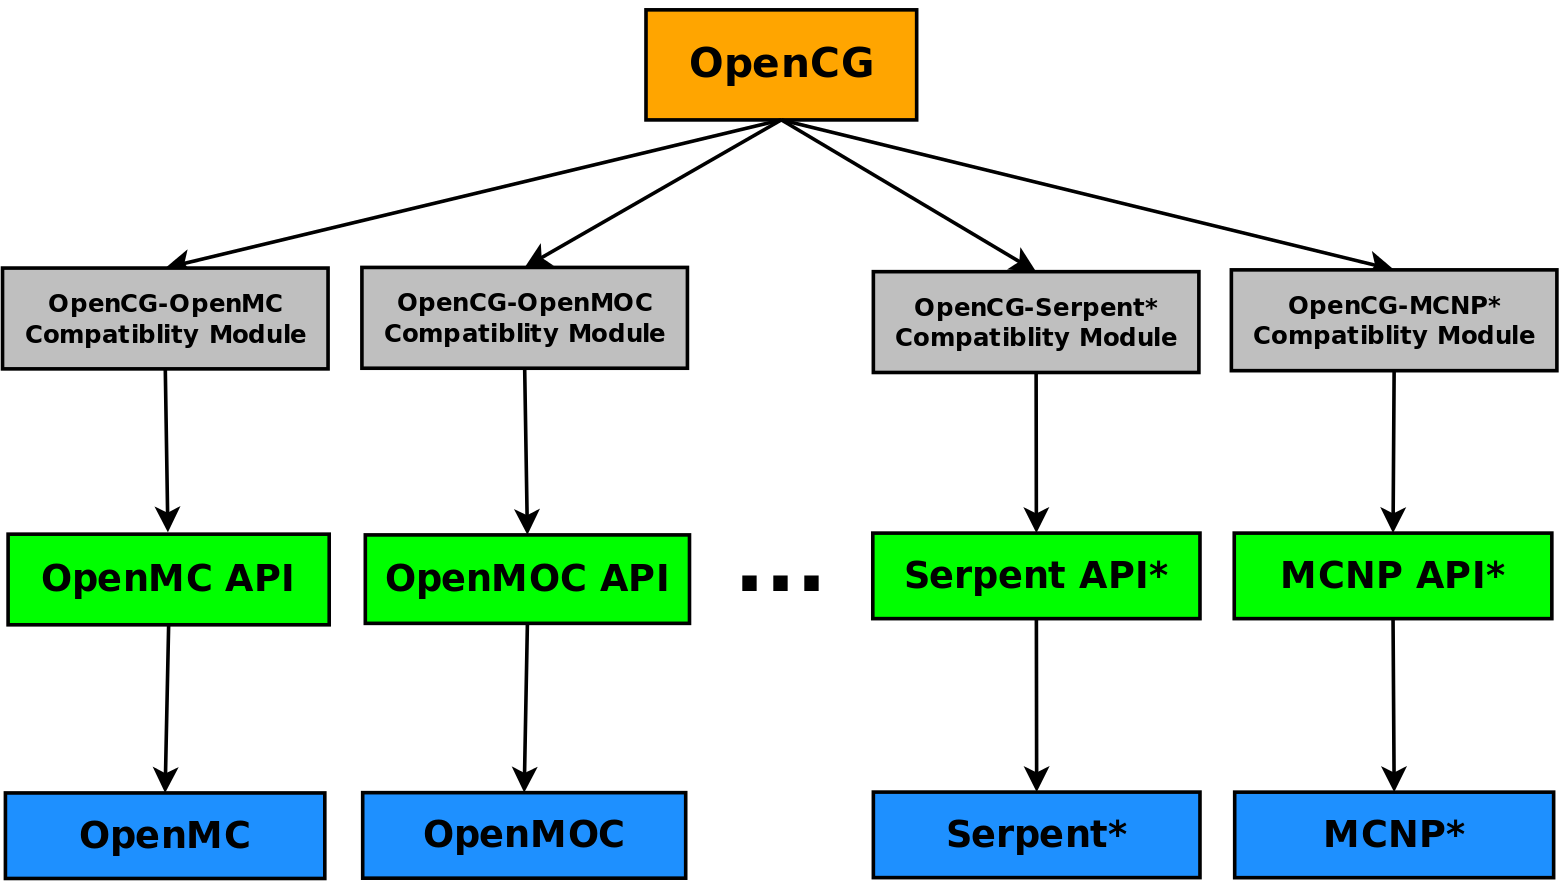
\includegraphics[width=.8\linewidth]{figures/workflow/opencg/compatibility-modules}
%  \caption{OpenCG compatibility modules for various neutron transport codes. The compatibility modules for OpenMC and OpenMOC will be released in future public distributions of each code, while modules for Serpent and MCNP are in progress at the time of this writing.}
%  \label{fig:compatibility-modules}
%\end{figure}


%%%%%%%%%%%%%%%%%%%%%%%%%%%%%%%%%%%%
\subsection{Local Neighbor Symmetry}
\label{sec:chap4-lns}

One of the unique algorithms implemented in OpenCG explicitly for this thesis is known as Local Neighbor Symmetry (LNS) identification~\cite{boyd2015opencg}. The LNS algorithm is motivated by this thesis' objective to accurately predict spatial zones that experience similar spectral self-shielding effects. The \ac{LNS} algorithm performs a systematic analysis of a \ac{CG} tree data structure to identify neighbor cells, or pairs of cells which are adjacent to one another. The neighbor cells are assembled into a heuristic which groups like spatial zones with common \ac{LNS} identifiers. The \ac{LNS} algorithm is analogous to the geometric templates used in lattice physics codes such as CASMO~\cite{edenius1995casmo} to identify fuel pins which have similar \ac{MGXS} in a fuel assembly.

The \ac{LNS} algorithm identifies the unique symmetry for the path to a region in a combinatorial geometry as described in Alg.~\ref{alg:local-neighbor-symmetry-cells}. \ac{LNS} performs a \ac{BFS} to find neighbors on each level of the \ac{CG} tree. For example, \ac{BFS} is used to find neighbor cells for a particular cell within a universe. Similarly, \ac{BFS} is used to find neighbor universes adjacent to a particular lattice cell. The neighbor cells and universes on each of the $k$ levels of a \ac{CG} tree are connected to form a $k$-partite graph\footnote{A $k$-partite graph is a graph whose graph vertices can be partitioned into $k$ disjoint sets so that no two vertices within the same set are adjacent~\cite{weisstein2012kpartite}.} as depicted in Fig.~\ref{fig:lns-k-partite-graph}. Finally, the $k$-partite graph is used as an argument to a hash function to compute the \ac{LNS} identifier (\textit{e.g}, a non-negative integer) for the particular region represented by the path. This algorithmic formulation is general to any arbitrary combinatorial geometry, including those commonly used to model \ac{LWRs} with nested rectilinear lattices.

\begin{algorithm}[h!]
\caption[OpenCG's Local Neighbor Symmetry Identification]{Local Neighbor Symmetry Identification}
\label{alg:local-neighbor-symmetry-cells}
\begin{algorithmic}[1]
\Procedure{computeNeighborSymmetry}{$path$}
    \State $G \gets \emptyset$ \Comment{Initialize empty set for graph}
    \State $k \gets$ \textbf{length}($path$) \Comment{Find number of independent sets}
    \For{$i := 1, k$}
        \If{\textbf{type}($path[i]$) \textbf{is} UNIVERSE}
            \State $G \gets G \cup \{path[i]\}$ \Comment{Append universe to graph}
        \ElsIf{\textbf{type}($path[i]$) \textbf{is} LATTICE}
            \State $N \gets$ \Call{BreadthFirstSearch}{$path[i]$} \Comment{Find lattice cell neighbors}
            \State $G \gets G \cup \{N\}$ \Comment{Append neighbors to graph}
        \ElsIf{\textbf{type}($path[i]$) \textbf{is} CELL}
            \State $N \gets$ \Call{BreadthFirstSearch}{$path[i]$} \Comment{Find cell neighbors}
            \State $G \gets G \cup \{N\}$ \Comment{Append neighbors to graph}
        \EndIf
    \EndFor
    \State \textbf{return} \Call{Hash}{$G$} \Comment{Return $k$-partite graph hash}
\EndProcedure
\end{algorithmic}
\end{algorithm}

\begin{figure}[h!]
  \centering
  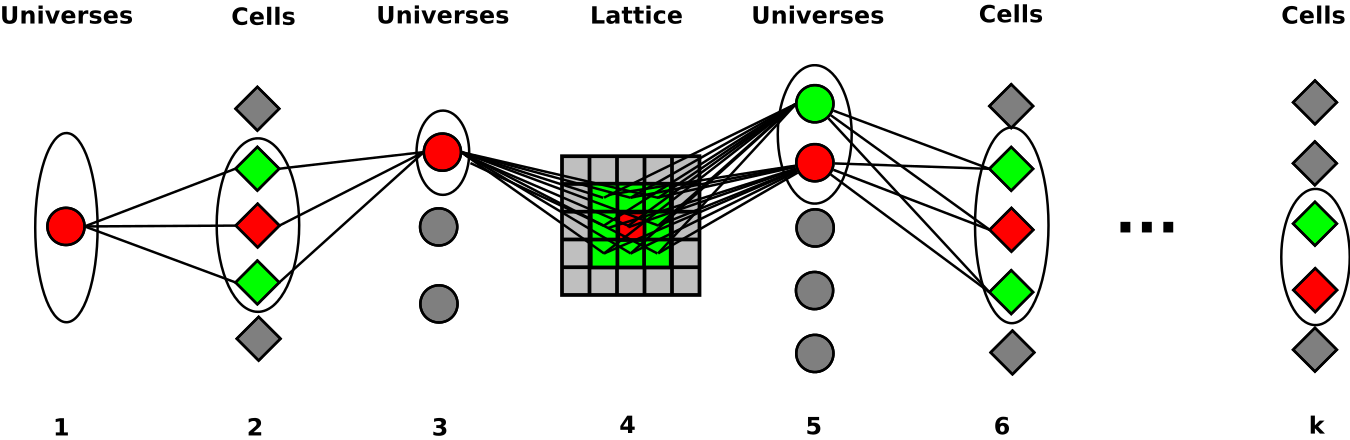
\includegraphics[width=\linewidth]{figures/workflow/opencg/neighbors-k-partite-graph}
  \caption[A $k$-partite graph created by the OpenCG LNS algorithm]{An example $k$-partite graph structure used to identify local neighbor symmetries. Red nodes correspond to the universes/cells encapsulating a region of interest, green nodes correspond to the neighbors of that region, and gray nodes correspond to universes/cells which are not neighbors. Red and green nodes at each level are combined into an argument for a hash function to generate a \ac{LNS} ID for the region of interest.}
  \label{fig:lns-k-partite-graph}
\end{figure}

Several parameters are incorporated into OpenCG's \ac{LNS} \ac{API} to provide the user with various methods to adjust the number of symmetries discovered by the algorithm. For example, OpenCG includes \textit{general} and \textit{unique} neighbor identifiers. General neighbors includes all neighbor cells/universes found by \ac{BFS} -- including duplicates -- as separate nodes in the $k$-partite graph. For example, a single universe may be placed multiple times around a lattice cell, each instance of which will be independently discovered by \ac{BFS} and replicated as a distinct node within the graph. On the contrary, unique neighbors does not include duplicate cells/universes -- only unique cells/universes are represented by distinct nodes in each independent set in the $k$-partite graph. A few diagrams of general and unique \ac{LNS} applied to two geometries are depicted in Fig.~\ref{fig:neighbor-cells}.

\begin{figure}[h!]
\begin{subfigure}{.5\textwidth}
  \centering
  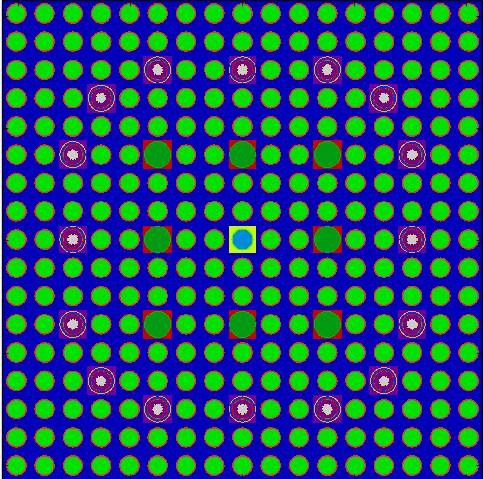
\includegraphics[width=.7\linewidth]{figures/workflow/opencg/cells-xy-24-16-assm}
  \caption{}
  \label{fig:assm-cells}
\end{subfigure}%
\begin{subfigure}{.5\textwidth}
  \centering
  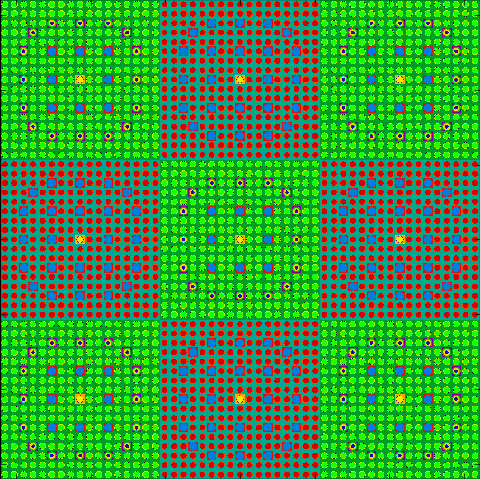
\includegraphics[width=.7\linewidth]{figures/workflow/opencg/cells-xy-colorset}
  \caption{}
  \label{fig:colorset-cells}
\end{subfigure}
\begin{subfigure}{.5\textwidth}
  \centering
  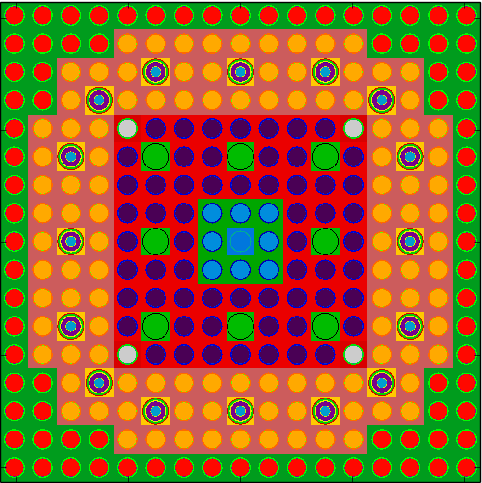
\includegraphics[width=.7\linewidth]{figures/workflow/opencg/unique-neighbor-cells-xy-24-16-assm}
  \caption{}
  \label{fig:assm-unique-neighbors}
\end{subfigure}
\begin{subfigure}{.5\textwidth}
  \centering
  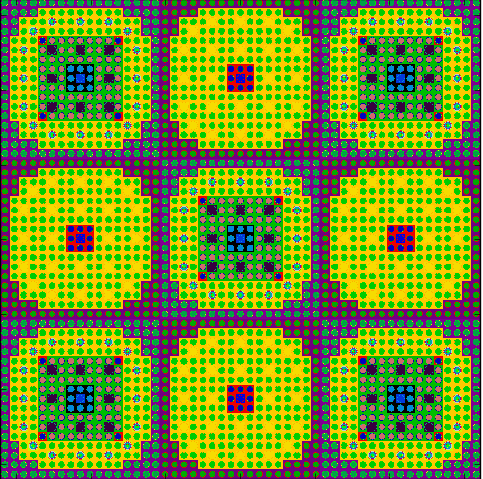
\includegraphics[width=.7\linewidth]{figures/workflow/opencg/unique-neighbor-cells-xy-colorset}
  \caption{}
  \label{fig:colorset-unique-neighbors}
\end{subfigure}
\begin{subfigure}{.5\textwidth}
  \centering
  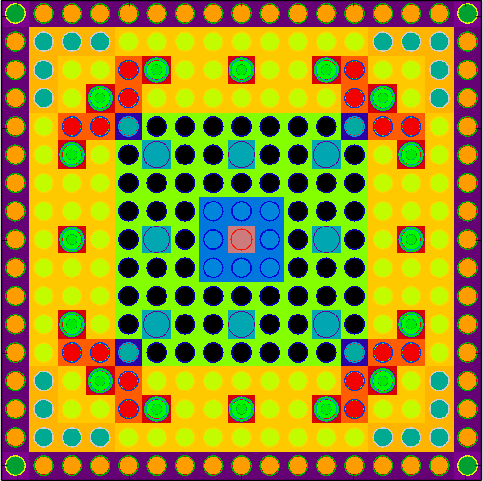
\includegraphics[width=.7\linewidth]{figures/workflow/opencg/neighbor-cells-xy-24-16-assm}
  \caption{}
  \label{fig:assm-neighbors}
\end{subfigure}
\begin{subfigure}{.5\textwidth}
  \centering
  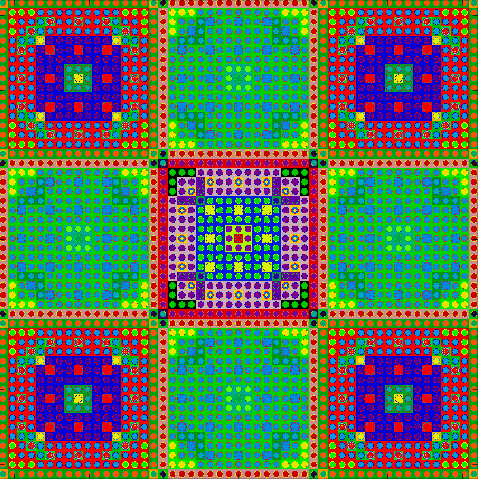
\includegraphics[width=.7\linewidth]{figures/workflow/opencg/neighbor-cells-xy-colorset}
  \caption{}
  \label{fig:colorset-neighbors}
\end{subfigure}
\caption[Example OpenCG Local Neighbor Symmetry mappings]{Two rectilinear lattice geometries are depicted to illustrate the use of local neighbor symmetry identification~\cite{boyd2015opencg}. The \textit{cells} are depicted for (a) a 17$\times$17 PWR lattice and (b) a 3$\times$3 colorset of two different 17 $\times$ 17 PWR assemblies each with burnable absorbers, guide tubes and instrument tubes. The \textit{unique neighbor} symmetry identifiers are color-coded in (b) and (c) for the assembly and colorset, respectively. Likewise, the \textit{general neighbor} symmetry identifiers are color-coded in (d) and (f).}
\label{fig:neighbor-cells}
\end{figure}

To this author's knowledge there is no other implementation of \ac{LNS} aside from that in the OpenCG code. The \ac{LNS} algorithm was used extensively in this thesis as a deterministic ``clustering'' technique for the spatial homogenization methodology introduced in Chaps.~\Crefrange{chap:benchmarks}{chap:unsupervised}. In particular, \ac{LNS} was used to predict which fuel pins have similar \ac{MGXS} in \ac{LWRs} due to spatial self-shielding effects induced by neighboring fuel, guide tube and absorber pins. The \ac{LNS} scheme served as a proxy to the traditional geometric template approach used in lattice physics codes to group pins with like \ac{MGXS}. The spatial homogenization methodology developed in Chaps.~\Crefrange{chap:benchmarks}{chap:unsupervised} incorporates \ac{MC} tally data in unsupervised clustering in an attempt to outperform \ac{LNS}' analysis based solely on the geometry.


%%%%%%%%%%%%%%%%%%%%%%%%%%%%%%%%%%%%
\subsection{Region Differentiation}
\label{sec:chap4-region-diff}

As previously noted, one of the advantages of combinatorial geometry is that it can take advantage of patterned structures with repeating primitives. In certain use cases, however, it may be necessary to replicate certain primitives which have the same geometric properties but experience very different radiation and/or thermal hydraulic conditions, and hence have different material properties in a transport simulation. For example, the \ac{LNS} algorithm is useful for identifying groups of fuel pin cell instances which may have similar \ac{MGXS}. However, in order for a transport code to make use of \ac{LNS}, a replica of each cell must be made to represent each of its different \ac{LNS} identifiers.

%first paragraph: motivation
%-build combinatorial geometries based on arbitrary clustering of cell instances

The process of manually constructing a \ac{CG} with many replicated but geometrically identical cells is very time consuming and prone to errors. To address this issue, a novel algorithm termed \textit{region differentiation} was implemented in OpenCG to efficiently and systematically reconstruct a \ac{CG} with replicated cells~\cite{boyd2015opencg}. A characterization of the region differentiation algorithm applied to a \ac{CG} tree data structure is shown in Fig.~\ref{fig:region-differentiation}.

The region differentiation algorithm is implemented in OpenCG and presents an interface which takes in a set of arbitrarily formed \textit{region groupings}. A region grouping is the set of all regions, that reference a particular cell in the geometry. Alternatively, a region grouping can be thought of as a set of repeated instances of a cell throughout a combinatorial geometry. Two or more region groupings corresponding to the same cell designate specific cell instances that should be replicated. The region differentiation algorithm replicates cells, universes, and lattices for each region grouping.

A naive or brute-force implementation of the region differentiation algorithm would scale as $\mathcal{O}(kn!)$ in both memory and time for $k$ nested universe/cell levels and $n$ region groupings. The reason is that \textit{a priori}, the algorithm does not know from which region groupings various cell instances will combine with one another to form universes, lattices and/or cells, which must themselves be differentiated for each possible combination of region groupings. To avoid factorial scaling, OpenCG makes use of dynamic programming to efficiently differentiate primitives one level at a time within the geometry.

\afterpage{\clearpage}
\begin{figure}[p]
\begin{subfigure}{\textwidth}
  \centering
  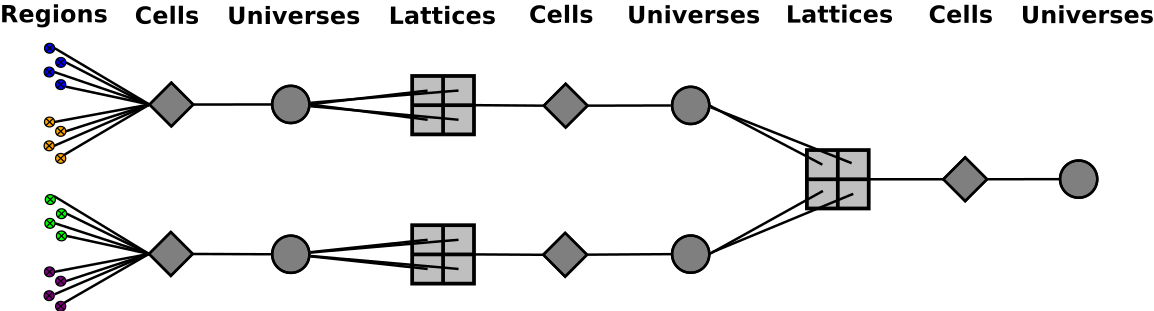
\includegraphics[width=0.82\linewidth]{figures/workflow/opencg/region-differentiation-1}
  \caption{}
  \label{fig:differentation-1}
\end{subfigure}
\begin{subfigure}{\textwidth}
  \centering
  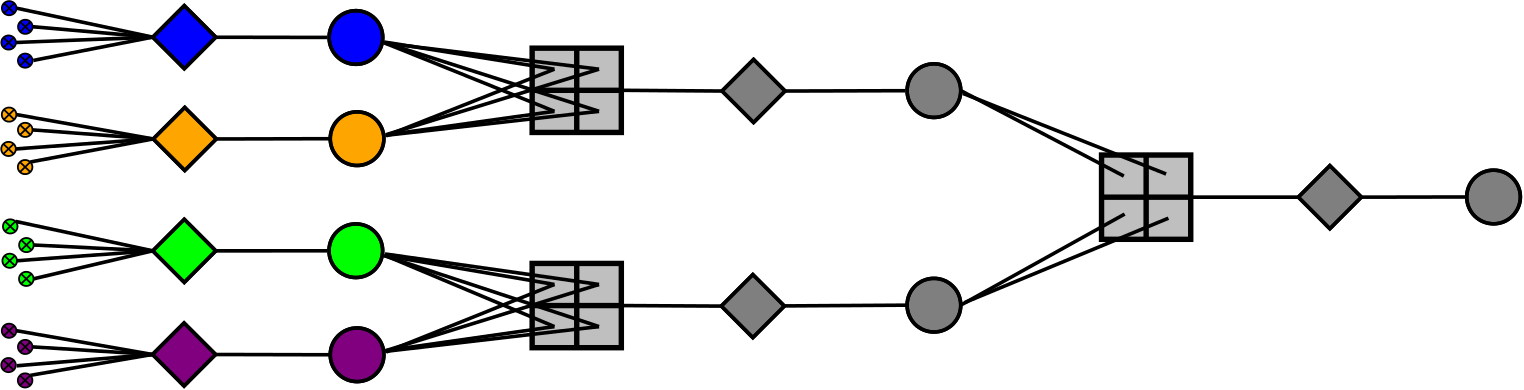
\includegraphics[width=0.75\linewidth]{figures/workflow/opencg/region-differentiation-2}
  \caption{}
  \label{fig:differentation-2}
\end{subfigure}
\begin{subfigure}{\textwidth}
  \centering
  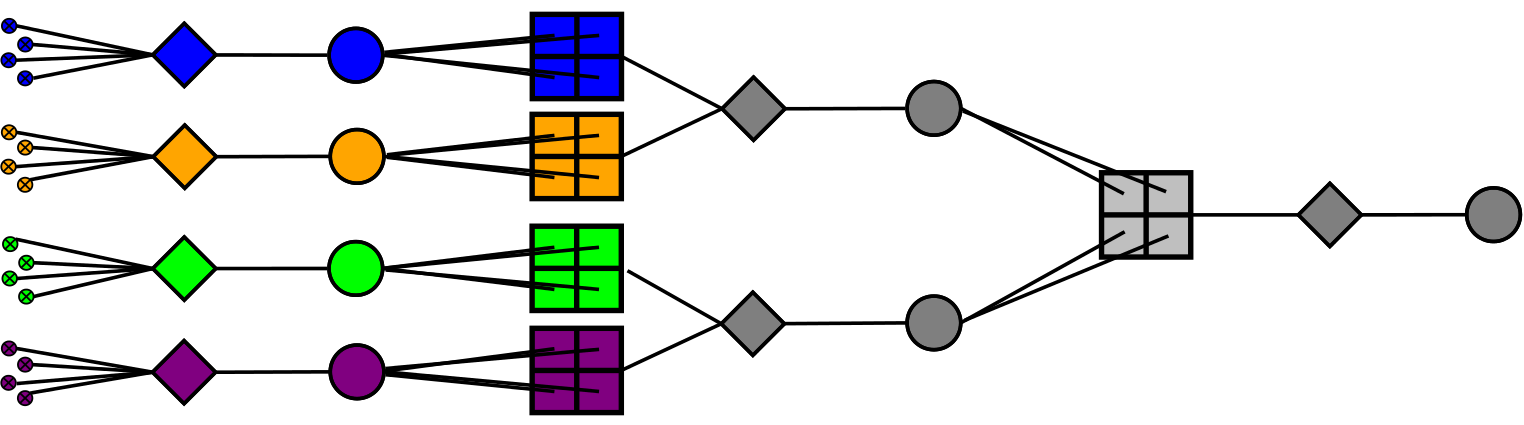
\includegraphics[width=0.75\linewidth]{figures/workflow/opencg/region-differentiation-3}
  \caption{}
  \label{fig:differentation-3}
\end{subfigure}
\begin{subfigure}{\textwidth}
  \centering
  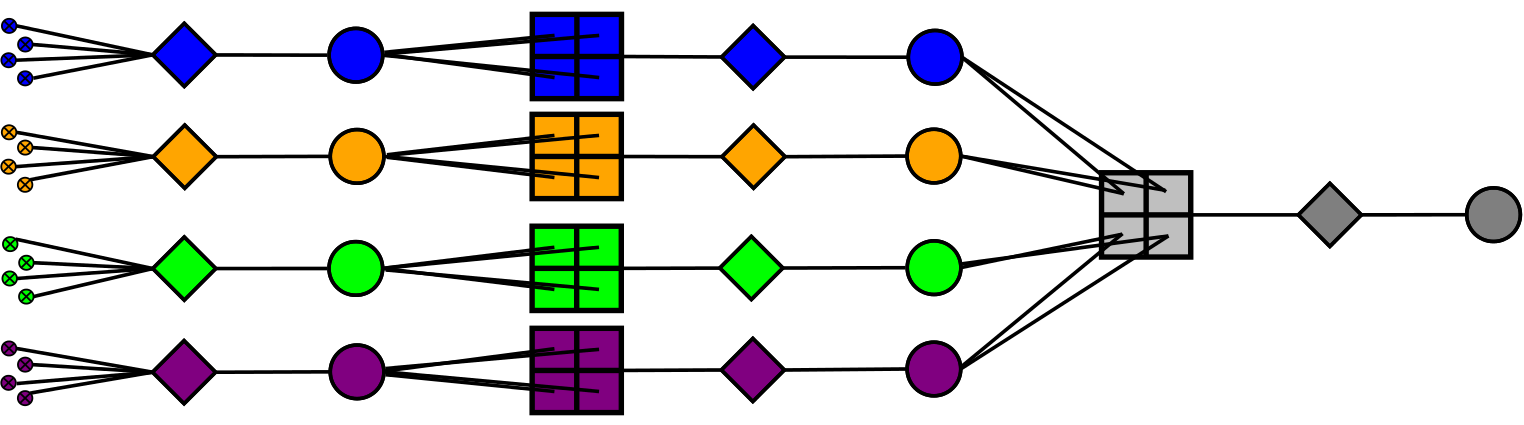
\includegraphics[width=0.75\linewidth]{figures/workflow/opencg/region-differentiation-4}
  \caption{}
  \label{fig:differentation-4}
\end{subfigure}
\begin{subfigure}{\textwidth}
  \centering
  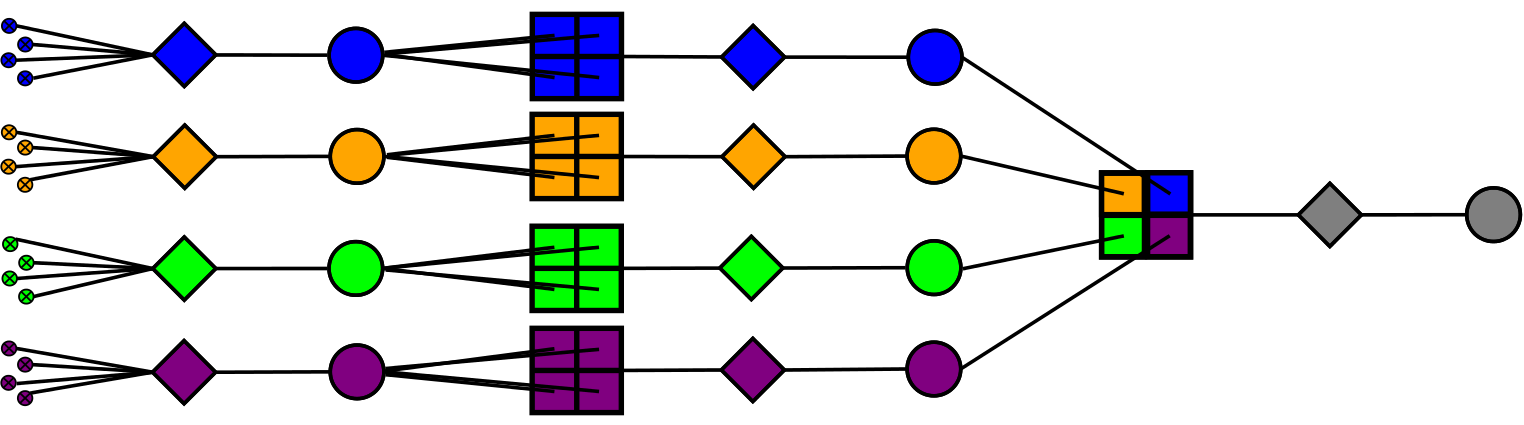
\includegraphics[width=0.75\linewidth]{figures/workflow/opencg/region-differentiation-5}
  \caption{}
  \label{fig:differentation-5}
\end{subfigure}
\caption[A few stages of the OpenCG region differentiation algorithm]{A few of the stages of the region differentiation algorithm~\cite{boyd2015opencg}. The regions (cell instances) to be differentiated are grouped and colored blue, orange, green and purple in (a). The first levels of cells and universes for each region group are differentiated in (b). The same is done for the lattices in (c). The algorithm continues to recursively differentiate cells, universes and lattices until no region groups collide at any level of the CG tree in (e).}
\label{fig:region-differentiation}
\end{figure}

The region differentiation algorithm iterates over each level of nested universes and cells. At each step, the paths for each region starting from the current level in the \ac{CG} tree and ending with the root universe node are hashed and stored in a hash table linked to the region grouping. Next, the algorithm manages \textit{primitive collisions} when two or more region groupings with the same path in the hash table point to the same primitive (cell, universe or lattice). To resolve primitive collisions, the algorithm differentiates the primitive for each region grouping involved in the collision. As primitive collisions are resolved, the algorithm merges any region groupings with paths that hash to same value in the hash table. The algorithm's termination condition is reached when the hash table only has one entry -- \textit{i.e.}, paths for all regions hash to the same value.

The region differentiation algorithm was an indispensable component of the simulation triad used to explore novel \ac{MGXS} generation techniques in this thesis. In particular, region differentiation made it possible to rapidly construct geometries to reflect the assignment of \ac{MGXS} to arbitrary collections of fuel pins for the spatial homogenization methodology introduced in Chaps.~\Crefrange{chap:benchmarks}{chap:unsupervised}. Fig.~\ref{fig:region-diff-proc-diagram} illustrates a flow diagram where the \ac{LNS} algorithm identifies the region groupings input to the region differentiation algorithm. The geometry produced from region differentiation may then be exported for use in OpenMC or OpenMOC using the compatibility modules discussed in Sec.~\ref{sec:chap4-opencg-compatibility}.

\begin{figure}[h!]
  \centering
  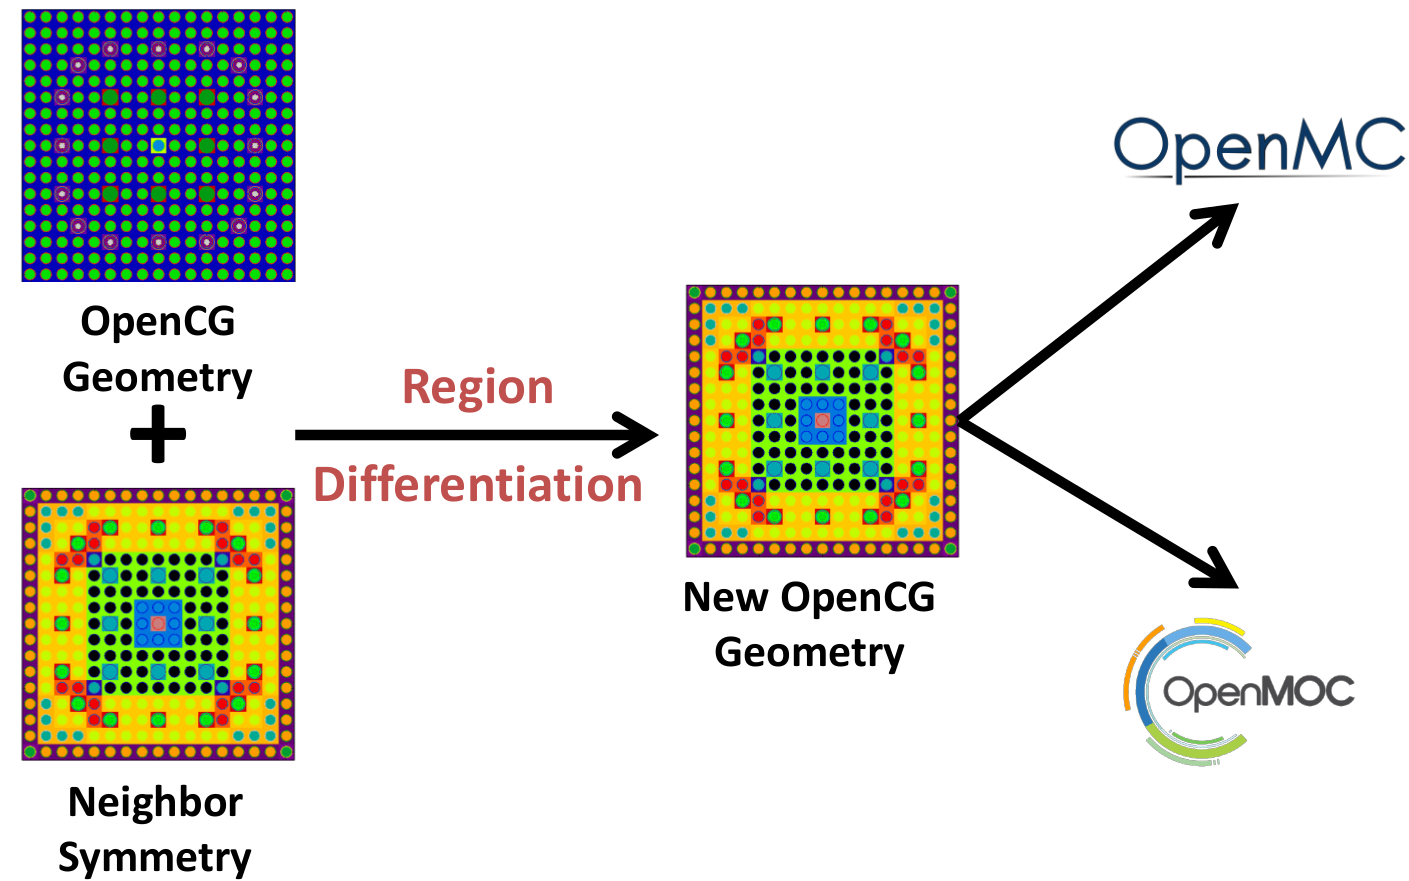
\includegraphics[width=0.8\linewidth]{figures/workflow/opencg/region-diff-proc-diagram}
  \caption[OpenCG region differentiation process diagram]{The OpenCG \ac{LNS} algorithm may be used to generate region groupings for the region differentiation algorithm to create a geometry for OpenMC or OpenMOC.}
  \label{fig:region-diff-proc-diagram}
\end{figure}

\begin{emphbox}
\textbf{The OpenCG code was implemented to facilitate data transfer between OpenMC and OpenMOC. The \ac{LNS} and region differentiation algorithms supported the novel spatial homogenization methodology developed in Chaps.~\Crefrange{chap:benchmarks}{chap:unsupervised}.}
\end{emphbox}


\vfill
\begin{highlightsbox}[frametitle=Highlights]
\begin{itemize}
  \item A framework consisting of the OpenMC, OpenMOC and OpenCG codes comprise a ``simulation triad'' used to explore \ac{MC}-based \ac{MGXS} generation methods for fine mesh transport calculations.
  \item A fully-featured Python \ac{API} was developed to support input generation and downstream processing of large tally datasets for OpenMC.
  \item The \texttt{openmc.mgxs} Python module was created to generate \ac{MGXS} from OpenMC tallies. The distributed cell tally algorithm was implemented to generate pin-wise \ac{MGXS} in large, heterogeneous geometries.
  \item New features were added to the deterministic multi-group OpenMOC code to enable it to use \ac{MGXS} generated by \texttt{openmc.mgxs} in 2D \ac{MOC} calculations.
  \item The OpenCG code was created to facilitate data processing and transfer on the combinatorial geometry meshes used by OpenMC and OpenMOC.
  \item OpenCG's \ac{LNS} and region differentiation algorithms were crucial components for the spatial homogenization methodology developed in Chaps.~\Crefrange{chap:benchmarks}{chap:unsupervised}.  
\end{itemize}
\end{highlightsbox}
\vfill

\part{Implementation}
% anals
\chapter{Software Design and Development}
\label{chap:software-design}

To implement the 3D MOC solver, the work in this thesis uses the OpenMOC~\ref{openmoc} neutron transport code. This code was developed initial for strictly 2D MOC simulations so great work was required to extend it to 3D MOC calculations. This chapter explains the structure of OpenMOC and the changes that were necessary to increase code flexibility to accommodate 3D MOC calculations. This chapter begins with a general overview of OpenMOC in Section~\ref{sec:openmoc-overview}. The interested reader can find a more complete description of the OpenMOC code in Boyd's thesis~\ref{boyd-ms}. Next, the object oriented design is discussed in greater detail in Section~\ref{sec:object-oriented} with a focus on the changes to accommodate both 2D and 3D simulations. In Section~\ref{sec:user-input} the standard Python user input is discussed as well as the new C++ alternative build which is attractive for high performance computing (HPC) applications where the availability of software required for the Python interface may be limited. Section~\ref{sec:version-control} concludes the chapter with a discussion of development practices and the open source license.

%%%%%%%%%%%%%%%%%%%%%%%%%%%%%%%%%%%%%%%%%%%%%%%%%%%%%%%%%%%%%%%%%%%%%%%%%%%%%%%%
\section{OpenMOC Overview}
\label{sec:openmoc-overview}

OpenMOC is neutron transport code that is written in C++ with a Simplified Wrapper Interface Generator (SWIG)~\cite{swig} to expose the C++ classes and routines to the Python scripting language. In this way, users are able to take advantage of the simplicity and flexibility of the Python language while also having the performance benefits of C++ compiled code. In this way users can work entirely in Python without having to touch the underlying C++ code and also do not have to learn a new input file syntax. This allows for users to write more natural code.

The underlying C++ code of OpenMOC also leverages the use of OpenMP~\cite{openmp} for shared memory parallelism. With the emergence of the 3D solver, distributed parallelism has also been implemented with MPI in the form of domain decomposition, discussed in Chapter~\ref{chap:domain-decomposition}. With this hybrid parallelism design, OpenMOC is able to scale to both many CPU cores and many nodes. 

OpenMOC is built on the use of constructive solid geometry (CSG), which allow complex geometries to be built out of boolean operations -- such as intersections and unions -- of simple surfaces and building blocks termed primitives. In addition, a hierarchy is used to agglomerate collections of primitives together. This approach is particularly useful for reactor geometries which are often highly structured. For example, a typical reactor core is built out of simple \textit{fuel pins}, grouped together into \textit{assemblies}. Assemblies are then grouped together to form the reactor core. An example of a CSG construction of a single assembly is given in Figure~\ref{fig:core-csg}.

\begin{figure}[h!]
	\centering
	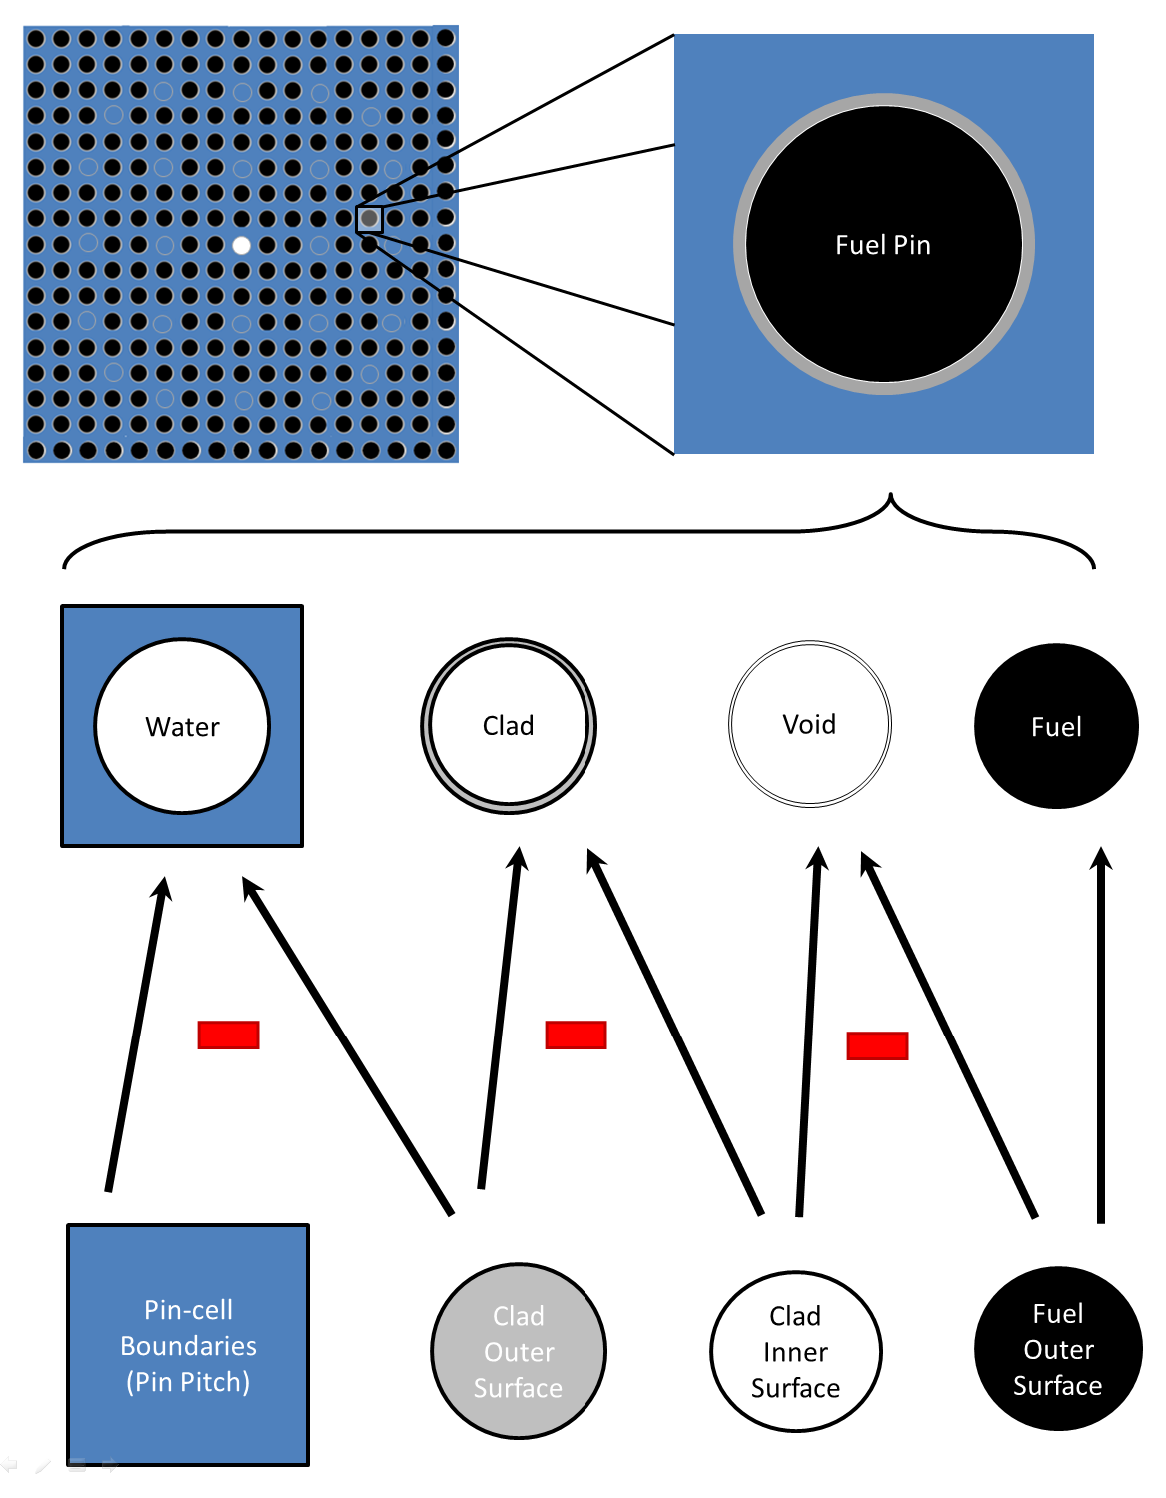
\includegraphics[width=0.9\linewidth]{figures/assembly-csg.PNG}
	\caption[]{The hierarchical CSG construction of a typical assembly.}
	\label{fig:core-csg}
\end{figure}

One of the benefits of the CSG approach is a reduced memory requirements of storing the geometry. Instead of explicitly storing information of each fuel pin within the reactor core, only unique fuel pin types need to be stored. They are then referenced in their parent object. For instance, an assembly contains an lattice of fuel pins. It would contain a mapping of location within the lattice to the unique assembly type, rather than the full information of each fuel pin.

In addition, the formation of a CSG allows ray tracing to be conducted in a general framework, agnostic of the individual primatives. Each \textit{cell} in OpenMOC is comprised of \textit{surface} objects and the half-space of each surface. A half-space determines on which side of the surface the cell is located. Ray tracing fundamentally involves calculating the distance to intersection along a direction. With the CSG framework, each of the bounding surfaces is queried for the distance to intersection. This naturally speeds up ray tracing by not having to check each instance of a surface within the geometry, but rather only the local surfaces. 

Once the geometry is built, OpenMOC generates tracks across the constructed geometry, and solves the neutron transport equation iteratively, as described in Chapter~\ref{chap:moc}. CMFD acceleration can also be included by the user, which employs the underlying methods that were described in Chapter~\ref{chap:cmfd-acceleration}.

Once the neutron transport equation is solved, the solver can be queried to return the scalar flux distribution. In order to visualize the data, OpenMOC includes Python plotting routines for scalar flux data, computed reaction rates, as well as geometric detail and visual diagnostics. 


%%%%%%%%%%%%%%%%%%%%%%%%%%%%%%%%%%%%%%%%%%%%%%%%%%%%%%%%%%%%%%%%%%%%%%%%%%%%%%%%
\section{Object Oriented Design}
\label{sec:object-oriented}

OpenMOC uses the object oriented programming paradigm whereby data structures called \textit{classes} are created that encapsulate both the data and associated subroutines. Object oriented programming generally leads to more resilient code since only the class itself can access its private attributes. An instantiation of a class is termed an \textit{object}. OpenMOC applies many of the principles of object oriented programming including information hiding, inheritance, and polymorphism.

An OpenMOC simulation requires three main components: a geometry, a track generator, and a solver. All of these are C++ classes in OpenMOC and exposed to the user. The user first describes the surfaces, cells, universes, and materials which constitute the geometry in a hierarchical CSG arrangement. The user then instantiates a \texttt{Geometry} object and provides it the root cell of the CSG. Next, a \texttt{TrackGenerator} is instantiated which is provided the \texttt{Geometry} object as well as track generation parameters such as radial ray spacing and number of azimuthal angles. Lastly, a \texttt{Solver} object is instantiated and given the \texttt{TrackGenerator} object along with solver criteria such as the tolerance. The solver can then be called to solve the MOC equations, such as the MOC neutron transport eigenvalue problem.

Extending the OpenMOC solver to 3D simulations required restructuring all of these classes in order to make them more flexible. The goal in extending to 3D simulations was to still maintain the ability to run 2D simulations, if desired. Additionally, to make the code more resilient and simpler, common code reuse should be maximized. Many of the routines present in the 2D simulations would also be used in the 3D simulations so both should use the same code without re-writing those entire sections. Also, users might be interested in running both 2D and 3D simulations on the same problem. Therefore, the input structure should not change much between 2D and 3D simulations. These points illustrate that the code should aim for maximum cohesion between the 2D and 3D modes. This is accomplished by expanding the 2D classes to be more general.

\subsection{\texttt{Geometry} Class Updates}
\label{sec:oo-geometry}

The \texttt{Geometry} class is altered to accommodate piecewise \textit{extruded geometries}. Extruded geometries are configurations in which the geometry looks the same at every axial level. A piecewise extruded geometry is a geometry that can be formed as the union of a finite number of extruded geometries. For instance, a fuel rod with end caps would fit the description of an extruded geometry but a sphere would not. Most practical reactor applications are indeed piecewise extruded geometries so this is not a very strong limitation. 

With the change from 2D geometries to piecewise axially extruded geometries, circles are transformed to $z$-cylinders (cylinders with the major axis vertical) and $z$-planes are added with a similar structure to the $x$ and $y$ planes already incorporated in OpenMOC. With this new geometry paradigm, 2D problems are thought of as simulating an $xy$ slice of a 3D geometry at a given $z$ height. By default this height is assumed to be 0.0 in order to limit the complexity of user input for 2D simulations.

\subsection{\texttt{TrackGenerator} Class Updates}
\label{sec:oo-trackgenerator}

Since tracks are built on a 2D projection, the 3D track generator must have all the functionality of the regular 2D track generator.

\subsection{\texttt{Solver} Class Updates}
\label{sec:oo-solver}

Solver - CPUSolver

%%%%%%%%%%%%%%%%%%%%%%%%%%%%%%%%%%%%%%%%%%%%%%%%%%%%%%%%%%%%%%%%%%%%%%%%%%%%%%%%
\section{Modular Structure}
\label{sec:modular-structure}

code reuse

For example, MOC can largely be described as an algorithm that performs a ray trace then computes equations over the segments formed from the ray trace. Many different ray tracing algorithms could be used with the underlying equations and solver remaining theoretically unchanged. However, if the code is rigid, each new ray tracing algorithm would require an entire code re-write. 

Talk about ray tracer comparison as a possibility

%%%%%%%%%%%%%%%%%%%%%%%%%%%%%%%%%%%%%%%%%%%%%%%%%%%%%%%%%%%%%%%%%%%%%%%%%%%%%%%%
\section{User Input}
\label{sec:user-input}

In terms of input structure, the 3D MOC updates to OpenMOC were structured to minimize the amount of work required to convert a 2D input to a 3D input. From a fully defined 3D geometry, including $z$-planes, the only difference in input between a 2D and 3D simulation is the definition of the track generator. A regular 2D \texttt{TrackGenerator} object supplied to a solver will trigger the 2D MOC solver, whereas a \texttt{TrackGenerator3D} object will trigger the 3D MOC solver.

If the Geometry was written in two dimensions without specifying $z$-planes, the geometry will need to be bounded in order to have a well defined 3D MOC problem. In theory, a 2D simulation implies infinite dimensions axially so if a bounded 3D geometry is provided to a regular 2D \texttt{TrackGenerator} object, a warning will be triggered, but the simulation will still run assuming infinite axial dimensions.

To facilitate running on systems which do not have thorough Python support or have difficulty transferring MPI communicator objects between Python and C++ for domain decomposed simulations, an alternative C++ build was implemented. This build uses a standard C++ Makefile and includes sample inputs in C++.

%%%%%%%%%%%%%%%%%%%%%%%%%%%%%%%%%%%%%%%%%%%%%%%%%%%%%%%%%%%%%%%%%%%%%%%%%%%%%%%%%
\section{Version Control and Licensing}
\label{sec:version-control}

OpenMOC utilizes Git version control and an open source distribution is hosted on GitHub at \url{https://github.com/mit-crpg/OpenMOC.git}. Git is a free and open source version control distribution that is becoming the software industry standard for version control. GitHub uses the Git distribution to host software distributions, both open source and closed source. Pull requests to the \textit{develop} branch form the basis by which the code evolves. Anyone in the public can contribute to the code by making a pull request to the develop branch. 

The OpenMOC code has been approved for open source release by the MIT Technology Licensing Office (TLO) under the MIT/X license. This license allows anyone to download the software without restriction. In addition, modifications to the software may be published, distributed, or sold. OpenMOC is designed with the intent of experimenting with new ideas within MOC simulations. This is further aided by the new flexible structure detailed in this chapter. The goal of OpenMOC is to promote an active reactor physics community where transparent research is possible and new ideas encourage the improvement of nuclear reactor modeling and simulation.
\chapter{Quantification of Spatial Self-Shielding Effects}
\label{chap:quantify}


%%%%%%%%%%%%%%%%%%%%%%%%%%%%%%%%%%%%%%%%%%%%%%%%%%%%%%%%%%%%%%%%%%%%%%%%%%%%%%%
\section{Overview}
\label{sec:chap8-overview}

The preceding chapter introduced six heterogeneous 2D \ac{PWR} benchmarks derived from the \ac{BEAVRS} model, along with reference metrics tallied by OpenMC. This chapter applies multi-group transport calculations to model the same benchmarks in OpenMOC with \ac{MGXS} generated by OpenMC. The objective is to identify the bias between OpenMC and OpenMOC for \ac{MGXS} libraries which account for spatial self-shielding effects\footnote{The effects of neighboring pins, burnable poisons, reflectors and the core baffle, barrel and vessel are all of interest in the context of spatial self-shielding in this and subsequent chapters.} to varying degrees. In particular, this chapter quantifies the difference in the approximation error between simulations in which the same \ac{MGXS} are used in each unique fuel pin (\textit{e.g.}, each fuel enrichment) and those in which unique \ac{MGXS} are used in each and every pin. The former case does little if anything to model spatial self-shielding effects, whereas the latter case ``fully'' resolves these effects, albeit at the expense of very large \ac{MGXS} libraries. This difference in approximation error motivates the development of a novel methodology in the following chapters which uses statistical clustering to capture spatial self-shielding effects in \ac{MGXS}.

Three different schemes for spatial homogenization of pin-wise \ac{MGXS} are introduced in Sec.~\ref{sec:chap8-pinwise-space-homogenize} and are referred to as \textit{infinite}, \textit{null} and \textit{degenerate} spatial homogenization, respectively. The discretized models and runtime parameters used in the OpenMOC simulations are detailed in Sec.~\ref{sec:chap8-moc-params}. The bias between the OpenMOC simulations and the reference OpenMC results -- including eigenvalues, pin-wise fission rates and pin-wise U-238 capture rates -- are presented in Sec.~\ref{sec:chap8-mg-results}. The need for a new, more flexible and specialized approach to spatial homogenization which appropriately captures spatial self-shielding effects with minimal computational expense is discussed in Sec.~\ref{sec:chap8-motivate}.


%%%%%%%%%%%%%%%%%%%%%%%%%%%%%%%%%%%%%%%%%%%%%%%%%%%%%%%%%%%%%%%%%%%%%%%%%%%%%%%
\section{Pin-wise Spatial Homogenization Schemes}
\label{sec:chap8-pinwise-space-homogenize}

This chapter employs three different spatial homogenization schemes to model spatial self-shielding effects in \ac{MGXS}. Although all spatial zones may experience spatial self-shielding, this chapter only models the impact of spatial self-shielding on \ac{MGXS} in fissile regions. The infinite, null and degenerate spatial homogenization schemes are introduced in Secs.~\Crefrange{subsec:chap8-infinite}{subsec:chap8-degenerate}. These schemes model spatial self-shielding for each fuel pin with increasing granularity and complexity. The total number of materials (\textit{i.e.}, \ac{MGXS}) used to model each benchmark with each homogenization scheme is given in Tab.~\ref{table:chap8-num-materials}. A fuel assembly, 2$\times$2 colorset and part of the quarter core \ac{BEAVRS} model are color-coded by material and illustrated in Fig.~\ref{fig:chap8-homogenization-schemes} for each homogenization scheme.

The \texttt{openmc.mgxs} module (see Sec.~\ref{subsec:chap4-mgxs}) was used to compute 70-group \ac{MGXS} with OpenMC for each of the six heterogeneous benchmarks introduced in Chap.~\ref{chap:benchmarks}. The tallied \ac{MGXS} data was condensed to coarse 2-group and 8-group structures with downstream data processing as necessary. The OpenMC simulations were performed with 1000 batches with 10$^{6}$ particle histories per batch for each benchmark. This was only one tenth of the 10$^7$ histories per batch used to tally the reference results in Chap.~\ref{chap:benchmarks} for practical computational reasons\footnote{The total runtime consumed by OpenMC scales with the number of tallied quantities. The number of tallies used to compute \ac{MGXS} was much larger than the three used to compute the reference solutions in Chap.~\ref{chap:benchmarks}. As a result, the simulation time per history was prohibitively slow to generate \ac{MGXS} with the same number of histories as was used to compute the reference solution.}. Stationarity of the fission source was obtained with 200 inactive batches for the quarter core \ac{BEAVRS} model, while 100 inactive batches were employed for the other five benchmarks (see Sec.~\ref{subsec:chap7-src-stationarity}). OpenMC's ``iso-in-lab'' feature (see Sec.~\ref{subsec:chap4-iso-in-lab}) was employed to enable consistent comparisons between OpenMC's reference results and OpenMOC's calculations with an isotropic in lab scattering source.

\vspace{0.2in}

\begin{table}[h!]
  \centering
  \caption[Number of materials for each spatial homogenization scheme]{Number of materials modeled with unique \ac{MGXS} in each heterogeneous benchmark for each spatial homogenization scheme.}
  \small
  \label{table:chap8-num-materials}
  \vspace{6pt}
  \begin{tabular}{l r r r}
  \toprule
  \rowcolor{lightgray}
  & \multicolumn{3}{c}{\cellcolor{lightgray} \bf \# Fuel Materials} \\
  \multirow{-2}{*}{\cellcolor{lightgray} \bf Benchmark} &
  \multicolumn{1}{c}{\cellcolor{lightgray} \bf Infinite} &
  \multicolumn{1}{c}{\cellcolor{lightgray} \bf Null} &
  \multicolumn{1}{c}{\cellcolor{lightgray} \bf Degenerate} \\
  \midrule
1.6\% Assm & 1 & 1 & 264 \\
%1.6\% Assm & 5 & 5 & 268 \\
  \midrule
3.1\% Assm & 1 & 1 & 264 \\
%3.1\% Assm & 5 & 5 & 268 \\
  \midrule
3.1\% Assm w/ 20 BPs & 1 & 1 & 264  \\
%3.1\% Assm w/ 20 BPs & 7 & 7 & 270  \\
  \midrule
2$\times$2 Colorset & 2 & 2 & 1,056 \\
%2$\times$2 Colorset & 8 & 8 & 1,062 \\
  \midrule
2$\times$2 Colorset w/ Reflector & 2 & 2 & 1,056 \\
%2$\times$2 Colorset w/ Reflector & 8 & 8 & 1,062 \\
  \midrule
\ac{BEAVRS} Quarter Core & 3 & 3 & 12,993 \\ % 193 * 264 / 4. + 128 + 127 + 7 % 50,964
%\ac{BEAVRS} Quarter Core & 10 & 10 & 13,000 \\ % 193 * 264 / 4. + 128 + 127 + 7 % 50,964
  \bottomrule
\end{tabular}
\end{table}

\begin{figure}[h!]
\centering
\begin{subfigure}{.45\textwidth}
  \centering
  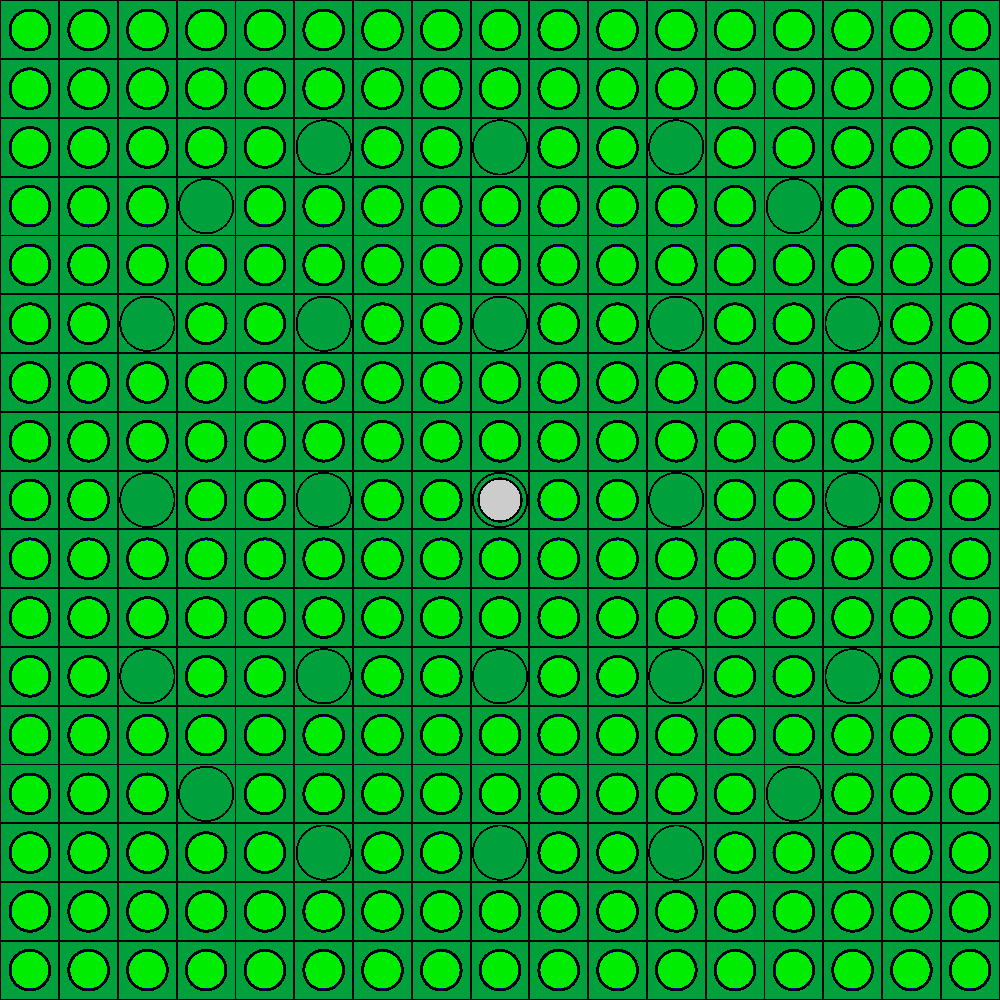
\includegraphics[width=0.87\linewidth]{figures/quantification/homogenization/assm-16-null-materials}
  \caption{}
  \label{fig:chap8-assm-16-null-materials}
\end{subfigure}%
\begin{subfigure}{.45\textwidth}
  \centering
  \includegraphics[width=0.87\linewidth]{figures/quantification/homogenization/assm-16-degenerate-materials}
  \caption{}
  \label{fig:chap8-assm-16-degenerate-materials}
\end{subfigure}
\begin{subfigure}{.45\textwidth}
  \centering
  \includegraphics[width=0.87\linewidth]{figures/quantification/homogenization/2x2-null-materials}
  \caption{}
  \label{fig:chap8-2x2-null-materials}
\end{subfigure}%
\begin{subfigure}{.45\textwidth}
  \centering
  \includegraphics[width=0.87\linewidth]{figures/quantification/homogenization/2x2-degenerate-materials}
  \caption{}
  \label{fig:chap8-2x2-degenerate-materials}
\end{subfigure}
\begin{subfigure}{.45\textwidth}
  \centering
  \includegraphics[width=0.87\linewidth]{figures/quantification/homogenization/full-core-null-materials}
  \caption{}
  \label{fig:chap8-full-core-null-materials}
\end{subfigure}%
\begin{subfigure}{.45\textwidth}
  \centering
  \includegraphics[width=0.87\linewidth]{figures/quantification/homogenization/full-core-degenerate-materials}
  \caption{}
  \label{fig:chap8-full-core-degenerate-materials}
\end{subfigure}
\caption[Depiction of spatial homogenization schemes]{OpenMOC materials for a single fuel assembly, a 2$\times$2 colorset and part of the 2D quarter core \ac{BEAVRS} model. The materials for the infinite and null schemes are depicted in (a), (c) and (e), and for the degenerate scheme in (b), (d) and (f), respectively. Each uniquely colored material represents a unique set of \ac{MGXS}.}
\label{fig:chap8-homogenization-schemes}
\end{figure}

%%%%%%%%%%%%%%%%%%%%%%%%%%%%%%%%%%%%%%
\subsection{Infinite Lattice Homogenization}
\label{subsec:chap8-infinite}

The \textit{infinite} spatial homogenization scheme is most reminiscent of the traditional multi-level schemes used to generate \ac{MGXS} (see Sec.~\ref{subsec:chap2-mgxs-lib-std-approach}), and is the simplest approach to model spatial self-shielding effects considered by this thesis. The infinite scheme employs multiple OpenMC simulations to compute \ac{MGXS} for each heterogeneous benchmark. The \ac{MGXS} for each type of fuel (\textit{e.g.}, enrichment) are generated by OpenMC simulations of each fuel pin type in an infinite, repeating array\footnote{An infinite, repeating array of fuel pins is modeled by a single fuel pin with reflective boundary conditions.}. The \ac{MGXS} for all other materials -- including borated water, zircaloy, helium, etc. -- are generated from OpenMC simulations of each heterogeneous benchmark where the reaction rates and fluxes are averaged across each geometry.

The infinite scheme is designed to quantify the impact of using the ``true'' Monte Carlo flux from an infinite lattice calculation, rather than the ``true'' \ac{MC} flux from the true heterogeneous geometry, to collapse \ac{MGXS} in fissile zones. The scheme employs a single \ac{MGXS} in each instance of a material zone, such as a fuel pin replicated many times throughout a benchmark geometry. The \ac{MGXS} for each fissile zone is generated from an infinite lattice calculation with OpenMC. The \ac{MGXS} for all non-fissile zones are generated using the ``true''  flux distribution in space and energy for each of the heterogeneous benchmarks. The scheme does not account for spatial self-shielding effects experienced by different non-fissile spatial zones filled by the same material, and instead averages these effects across the entire geometry for each material.

%-foonote: unable to run infinite pin cell calculations for non-fissile pin cells (CRGTs, BPs, instr tubes) since it's not a criticality calculation

%%%%%%%%%%%%%%%%%%%%%%%%%%%%%%%%%%%%%%
\subsection{Null Homogenization}
\label{subsec:chap8-null}

The \textit{null} spatial homogenization scheme builds upon the infinite scheme, but uses the ``true'' heterogeneous flux to collapse \ac{MGXS} for fissile as well as non-fissile materials. The null scheme eliminates the infinite lattice calculation to generate \ac{MGXS} for fissile zones, and instead uses a single Monte Carlo calculation of the complete heterogeneous geometry to generate \ac{MGXS} for \textit{all} materials. In this way, the null scheme fully abandons the multi-level approach used by the infinite scheme and most traditional approaches to generate \ac{MGXS}. Unlike the infinite scheme, the spatially self-shielded flux is used to collapse the cross sections in the fuel. However, the null scheme does not account for spatial self-shielding effects experienced by different fuel pins filled by the same type of fuel, and instead averages these effects across the entire geometry. As with the infinite scheme, a single \ac{MGXS} is employed in each instance of a material zone, such as a fuel pin replicated many times throughout a benchmark geometry.

%%%%%%%%%%%%%%%%%%%%%%%%%%%%%%%%%%%%%%
\subsection{Degenerate Homogenization}
\label{subsec:chap8-degenerate}

Unlike the infinite and null spatial homogenization schemes, the \textit{degenerate} scheme accounts for the different spatial self-shielding effects experienced by each instance of each fuel pin throughout a heterogeneous geometry. Like the null scheme, a single \ac{MC} calculation of the complete heterogeneous geometry is used to generate \ac{MGXS} for all materials. Unlike the null scheme, the \ac{MGXS} are tallied separately for each instance of fissile material zones. For example, if a heterogeneous benchmark includes $N$ fuel pins, then $N$ collections of \ac{MGXS} are separately tabulated for each fuel pin instance. The degenerate scheme tallies different \ac{MGXS} even if the isotopic compositions in the fuel pin instances are identical (\textit{e.g.}, fresh fuel at the beginning of life) since each instance may experience different spatial self-shielding effects and hence have different \ac{MGXS}.

Multi-group transport calculations with \ac{MGXS} generated using infinite/null and degenerate schemes may be compared to quantify the impact of modeling spatial self-shielding effects in \ac{MGXS} for fissile zones in heterogeneous geometries. The degenerate scheme applies the finest granularity to pin-wise spatial homogenization of any of the schemes considered in this thesis since it best captures different spatial self-shielding effects in each fuel pin. As a result, the degenerate scheme is used to benchmark the efficacy of the new methodology for spatial homogenization based on statistical clustering developed in the following chapters. Like both the infinite and null schemes, the spatial self-shielding effects experienced by different non-fissile spatial zones are averaged across the entire geometry for each non-fissile material.

The degenerate scheme generates \ac{MGXS} for each fuel pin instance using OpenMC's distributed cell tallies (see Sec.~\ref{subsec:chap4-distribcells}). The OpenCG region differentiation algorithm (see Sec.~\ref{sec:chap4-region-diff}) is used to build a new OpenMOC geometry with unique cells and materials for each fuel pin. The \ac{MGXS} are appropriately selected from OpenMC's distributed cell tallies to populate the \ac{MGXS} in the OpenMOC materials.

\begin{emphbox}
\textbf{The infinite, null and degenerate spatial homogenization schemes are used to quantify approximation errors made when neglecting spatial self-shielding due to neighboring pins, reflectors, etc. in heterogeneous \ac{PWR} benchmarks.}
\end{emphbox}


%%%%%%%%%%%%%%%%%%%%%%%%%%%%%%%%%%%%%%%%%%%%%%%%%%%%%%%%%%%%%%%%%%%%%%%%%%%%%%%
\section{OpenMOC Runtime Parameters}
\label{sec:chap8-moc-params}

The infinite, null and spatial homogenization schemes were used to prepare \ac{MGXS} libraries for OpenMOC simulations of each of the six heterogeneous \ac{PWR} benchmarks introduced in Chap.~\ref{chap:benchmarks}. This section briefly outlines the energy group structures and angular, spatial and \ac{CMFD} meshes used in the OpenMOC simulations. The total number of flat source regions, and \ac{MOC} tracks and segments are summarized for each benchmark in Tab.~\ref{table:chap8-num-fsrs-tracks-segments}. It was crucial to use an adequate discretization to accurately compare simulation results between the three spatial homogenization schemes, as well as to the reference OpenMC results.

\begin{table}[h!]
  \centering
  \caption[Number of FSRs, tracks and segments for each benchmark]{The number of \ac{MOC} \ac{FSR}s, tracks and segments modeled in each benchmark.}
  \small
  \label{table:chap8-num-fsrs-tracks-segments}
  \vspace{6pt}
  \begin{tabular}{l r r r}
  \toprule
  \rowcolor{lightgray}
  \textbf{Benchmark} &
  \multicolumn{1}{c}{\cellcolor{lightgray} \textbf{\# \ac{FSR}s}} &
  \multicolumn{1}{c}{\cellcolor{lightgray} \textbf{\# Tracks}} &
  \multicolumn{1}{c}{\cellcolor{lightgray} \textbf{\# Segments}} \\
  \midrule
1.6\% Assm & 28,376 & 34,976 & 7,945,952 \\
  \midrule
3.1\% Assm & 28,376 & 34,976 & 7,945,952 \\
  \midrule
3.1\% Assm w/ 20 BPs & 29,496 & 34,976 & 8,110,192  \\
  \midrule
2$\times$2 Colorset & 115,744 & 69,892 & 32,097,936 \\
  \midrule
2$\times$2 Colorset w/ Reflector & 203,220 & 104,788 & 51,122,228 \\
  \midrule
%\ac{BEAVRS} Quarter Core & 2,512,384 & 201,620 & 427,683,579 \\
\ac{BEAVRS} Quarter Core & 1,718,368 & 201,620 & 38,3785,515 \\
  \bottomrule
\end{tabular}
\end{table}

Each simulation was converged to 10$^{-5}$ on the root mean square of the energy-integrated fission source in each flat source region (FSR). It should be noted that a convergence criterion of 10$^{-7}$ was employed for the OpenMOC simulations of simple benchmarks without \ac{CMFD} acceleration (see Sec.~\ref{subsubsec:chap4-openmoc-cmfd}) in Chap.~\ref{chap:biases}, but a looser convergence criterion of 10$^{-5}$ may be used for calculations with \ac{CMFD}\footnote{The convergence criterion measures the residual between successive iterations, but should actually measure convergence to the asymptotic solution, which depends on both the residual between successive iterations and the dominance ratio. \ac{CMFD} significantly reduces the residual between successive iterations such that sufficient convergence to the asymptotic solution is achieved at a much lower successive iteration residual.}.

%%%%%%%%%%%%%%%%%%%%%%%%%%%%%%%%%%%%
\subsection{Energy Group Structures}
\label{subsec:chap8-energy-groups}

Each assembly, colorset and quarter core benchmark was modeled with \ac{MGXS} in 2, 8 and 70 energy groups. The energy group structures were the same as those used in Chaps.~\ref{chap:biases} and~\ref{chap:sph} and are tabulated in App.~\ref{app:energy-groups}. The \ac{MOC} energy group structures were collapsed onto coarser group structures for \ac{CMFD} acceleration. The mapping from \ac{MOC} to \ac{CMFD} group structures is listed in Tab.~\ref{table:chap8-coarse-cmfd-groups}. The coarse \ac{CMFD} structures were derived to best approximate equal lethargy spacing between coarse \ac{CMFD} groups. The coarse \ac{CMFD} structures significantly improved the speed of the 70-group OpenMOC calculations.

\begin{table}[h!]
  \centering
  \caption[CMFD coarse energy group structures]{The coarse \ac{CMFD} group structures for each of the fine \ac{MOC} group structures.}
  \small
  \label{table:chap8-coarse-cmfd-groups}
  \vspace{6pt}
  \begin{tabular}{p{1.5cm} p{1.5cm} p{7.2cm}}
  \toprule
  \rowcolor{lightgray}
  \multicolumn{1}{c}{\cellcolor{lightgray} \textbf{\# \ac{MOC} Groups}} &
  \multicolumn{1}{c}{\cellcolor{lightgray} \textbf{\# \ac{CMFD} Groups}} &
  \multicolumn{1}{c}{\cellcolor{lightgray} \textbf{\ac{CMFD} Fine-to-Coarse Group Mapping}} \\
  \midrule
  \multicolumn{1}{c}{2} & \multicolumn{1}{c}{2} & [1], [2] \\
  \midrule
  \multicolumn{1}{c}{8} & \multicolumn{1}{c}{4} & [1--2], [3], [4--5], [6--8] \\
  \midrule
%  \multicolumn{1}{c}{40} & \multicolumn{1}{c}{10} & [1--3], [4--7], [8], [9], [10], [11--13], \hspace{0.8cm} [14--16], [17--29], [30--36], [37--40] \\
%  \midrule
  \multicolumn{1}{c}{70} & \multicolumn{1}{c}{14} & [1--2], [3--6], [7--9], [10--12], [13--16], \hspace{0.6cm} [17--19], [20--21], [22--24], [25--27], [28--33], [34--53], [54--61], [62--68], [69--70] \\ 
  \bottomrule
\end{tabular}
\end{table}

%%%%%%%%%%%%%%%%%%%%%%%%%%%%%%%%%%%%
\subsection{Angular Discretization}
\label{subsec:chap8-angular-discretizations}

The OpenMOC simulations of each of the six heterogeneous benchmarks used the same \ac{MOC} angular discretization with 128 azimuthal angles and 0.05 cm track spacing. These parameters were selected since they were previously demonstrated to converge the solution for simple heterogeneous \ac{PWR} benchmark models~\cite{boyd2014ms}. Although the eigenvalues in Chap.~\ref{chap:biases} were only shown to converge for a 1D slab and 2D fuel pin with 0.01 cm track spacing, a coarser spacing of 0.05 cm was employed for the heterogeneous benchmarks for practical reasons\footnote{The computational expense of solving the \ac{MOC} equations scales linearly with the number of track segments. In addition, OpenMOC's memory footprint is dominated by track segments which can make some problems intractable except on high memory nodes. Finally, the time spent ray tracing across a combinatorial geometry is non-negligible if not prohibitive for fine track spacings in large geometries.}. The total number of tracks and segments resulting from the selected angular discretization are itemized in Tab.~\ref{table:chap8-num-fsrs-tracks-segments}. 

%%%%%%%%%%%%%%%%%%%%%%%%%%%%%%%%%%%%
\subsection{FSR Discretization}
\label{subsec:chap8-fsr-discretizations}

Flat source region spatial discretization meshes were applied to each of the six heterogeneous benchmarks in the OpenMOC simulations. The total number of \ac{FSR}s is itemized in Tab.~\ref{table:chap8-num-fsrs-tracks-segments} for each benchmark analyzed in this thesis. The \ac{FSR} meshes applied to the fuel pin, control rod guide tube, instrument tube and burnable poison pin cells are shown in Fig.~\ref{fig:chap8-pin-cell-fsrs}. As shown in the figures, eight equal angle subdivisions were used in all material zones. The UO$_2$ fuel was further subdivided into five equal volume radial rings, while ten radial rings were employed in the water-filled \acp{CRGT} and instrument tubes. The borosilicate glass and borated water material zones filling the \acp{BP} were each discretized into five equal volume radial rings. Finally, five equally spaced rings were used in the moderator zones surrounding each pin.

\begin{figure}[h!]
\centering
\begin{subfigure}{.5\textwidth}
  \centering
  \includegraphics[width=0.8\linewidth]{figures/quantification/fsrs/fsrs-fuel-pin}
  \caption{}
  \label{fig:chap8-pin-1.6}
\end{subfigure}%
\begin{subfigure}{.5\textwidth}
  \centering
  \includegraphics[width=0.8\linewidth]{figures/quantification/fsrs/fsrs-crgt}
  \caption{}
  \label{fig:chap8-pin-crgt}
\end{subfigure}
\begin{subfigure}{.5\textwidth}
  \centering
  \includegraphics[width=0.8\linewidth]{figures/quantification/fsrs/fsrs-instr-tube}
  \caption{}
  \label{fig:chap8-instr-tube}
\end{subfigure}%
\begin{subfigure}{.5\textwidth}
  \centering
  \includegraphics[width=0.8\linewidth]{figures/quantification/fsrs/fsrs-bp}
  \caption{}
  \label{fig:chap8-bp}
\end{subfigure}%
\caption[FSR discretization meshes applied to BEAVRS pin cells]{The \ac{FSR} spatial mesh used for fuel pins (a), control rod guide tubes (b), instrument tubes (c) and burnable poisons (d). Diagrams of each pin type color-coded by material are shown in Fig.~\ref{fig:chap7-pin-cells}.}.
\label{fig:chap8-pin-cell-fsrs}
\end{figure}

\begin{figure}[hb!]
\centering
\begin{subfigure}{0.45\textwidth}
  \centering
  \includegraphics[width=0.87\linewidth]{figures/quantification/fsrs/fsrs-assm-16}
  \caption{}
  \label{fig:chap8-assm-1.6-fsrs}
\end{subfigure}%
\begin{subfigure}{0.45\textwidth}
  \centering
  \includegraphics[width=0.87\linewidth]{figures/quantification/cmfd/cmfd-cells-assm}
  \caption{}
  \label{fig:chap8-assm-1.6-cmfd-cells}
\end{subfigure}
\begin{subfigure}{0.45\textwidth}
  \centering
  \includegraphics[width=0.87\linewidth]{figures/quantification/fsrs/fsrs-reflector}
  \caption{}
  \label{fig:chap8-reflector-fsrs}
\end{subfigure}%
\begin{subfigure}{0.45\textwidth}
  \centering
  \includegraphics[width=0.87\linewidth]{figures/quantification/cmfd/cmfd-cells-reflector}
  \caption{}
  \label{fig:chap8-reflector-cmfd-cells}
\end{subfigure}
\begin{subfigure}{0.45\textwidth}
  \centering
  \includegraphics[width=0.87\linewidth]{figures/quantification/fsrs/fsrs-full-core-quarter-pin-cmfd}
  \caption{}
  \label{fig:chap8-full-core-fsrs}
\end{subfigure}%
\begin{subfigure}{0.45\textwidth}
  \centering
  \includegraphics[width=0.87\linewidth]{figures/quantification/cmfd/cmfd-cells-full-core-quarter-pin-cmfd}
  \caption{}
  \label{fig:chap8-full-core-cmfd-cells}
\end{subfigure}
\caption[FSR discretization and CMFD cells for heterogeneous benchmarks]{\ac{FSR} (left) and \ac{CMFD} (right) meshes for a fuel assembly (a) and (b), a 2$\times$2 colorset with reflector (c) and (d), and quarter core \ac{BEAVRS} benchmark (e) and (f).}
\label{fig:chap8-assm-fsrs-cmfd-cells}
\end{figure}

The spatially discretized pin cells were used in each of the six heterogeneous benchmarks. The \ac{FSR} discretizations for an individual fuel assembly, 2$\times$2 colorset with a water reflector, and the upper right quadrant of the \ac{BEAVRS} core are depicted in Fig.~\ref{fig:chap8-assm-fsrs-cmfd-cells}. The water reflector in the 2$\times$2 colorset was discretized using a mesh shown to converge the solution for the similarly designed C5G7 benchmark~\cite{lewis2003c5g7} in~\cite{boyd2014ms}. In particular, the 13.85824 cm (equivalent to 11 pin cells) of water reflector nearest the fuel assemblies was discretized in a 0.125984 cm $\times$ 0.125984 cm rectilinear mesh, equivalent to a 10$\times$10 mesh in each pin. The 7.55904 cm (equivalent to 6 pin cells) of water reflector furthest from the fuel assemblies was discretized in a 1.25984 cm $\times$ 1.25984 cm pin-wise mesh.

Each type of pin cell was discretized in the same way for the quarter core \ac{BEAVRS} model. A 0.31496 cm $\times$ 0.31496 cm mesh (equivalent to a 4$\times$4 mesh in each pin) was applied in the water reflector. The mesh in the reflector was coarser than the mesh used in the reflector for the 2$\times$2 colorset since a finer mesh was not computationally practical for the quarter core \ac{BEAVRS} model, nor needed due to th presence of the steel baffle. A quarter pin-wise \ac{CMFD} mesh (\textit{i.e.}, 0.62992 cm $\times$ 0.62992 cm) was employed for the \ac{BEAVRS} model, which discretized the core barrel and vessel into a corresponding \ac{FSR} mesh.


%%%%%%%%%%%%%%%%%%%%%%%%%%%%%%%%%%%%%%%%%%%%%%%%%%%%%%%%%%%%%%%%%%%%%%%%%%%%%%%
\section{Analysis of Multi-Group Results}
\label{sec:chap8-mg-results}

Each of the six benchmarks was modeled with OpenMOC using \ac{MGXS} generated by the infinite, null and degenerate spatial homogenization schemes. The eigenvalues and pin-wise fission and U-238 capture rates computed by OpenMOC are compared to the reference OpenMC solutions in Secs.~\ref{subsec:chap8-eigenvalues},~\ref{subsec:chap8-fiss-rates} and~\ref{subsec:chap8-capt-rates}, respectively.

%%%%%%%%%%%%%%%%%%%%%%%%
\subsection{Eigenvalues}
\label{subsec:chap8-eigenvalues}

The OpenMOC eigenvalues were compared to the reference OpenMC eigenvalues from Tab.~\ref{table:chap7-ref-eigenvalues}. The eigenvalue bias $\Delta\rho$ was computed from Eqn.~\ref{eqn:chap5-delta-rho} in units of \ac{pcm}. The bias is listed for each benchmark, energy group structure and spatial homogenization scheme in Tab.~\ref{table:chap8-openmoc-eigenvalues}. It should be recalled that isotropic in lab scattering is used by OpenMC to compute both the reference solution and the \ac{MGXS}. If anisotropic scattering were employed in OpenMC, one would expect quite different biases without a robust implementation of a higher order scattering kernel in OpenMOC.

As expected, the eigenvalue bias is highly dependent on energy group structure. In general, a positive bias is exhibited for 2 groups with an increasingly negative trend with more groups. The bias is remarkably consistent between -100 and -250 \ac{pcm} for 70 groups for all of the benchmarks. This slightly negative bias is reminiscent of the -200 \ac{pcm} bias observed for the 1D slab and 2D pin cell \ac{PWR} benchmarks when modeled with 70 groups in Chap.~\ref{chap:biases}. The introduction of a reflector region in the 2$\times$2 colorset increases the bias to over 1700 \ac{pcm} for all homogenization schemes for 2 groups, but the bias is greatly reduced when modeled with more groups.

%\vspace{0.1in} 

\renewcommand{\arraystretch}{0.9}% Tighter

\begin{table}[ht!]
  \centering
  \caption[OpenMOC eigenvalue bias]{OpenMOC eigenvalue bias $\Delta\rho$ for heterogeneous benchmarks with varying spatial homogenization schemes and energy group structures.}
  \small
  \label{table:chap8-openmoc-eigenvalues}
  \vspace{6pt}
  \begin{tabular}{l l R{2.5cm} R{2.5cm} R{2.5cm}}
  \toprule
  \rowcolor{lightgray}
  & & \multicolumn{3}{S[table-format=6.1]}{\cellcolor{lightgray} {$\bm{\Delta\rho}$ \textbf{[pcm]}}} \\
  \multirow{-2}{*}{\cellcolor{lightgray} \bf Benchmark} &
  \multirow{-2}{*}{\cellcolor{lightgray} \bf \ac{MGXS} Scheme} &
  \multicolumn{1}{r}{{\cellcolor{lightgray} \bf 2-Group}} &
  \multicolumn{1}{r}{{\cellcolor{lightgray} \bf 8-Group}} &
  \multicolumn{1}{r}{{\cellcolor{lightgray} \bf 70-Group}} \\
  \midrule
\multirow{3}{*}{\parbox{2.5cm}{1.6\% Assm}} & Infinite & -132 & -68 & 31 \\
& Null & 60 & -72 & -161 \\
& Degenerate & 62 & -72 & -161 \\
  \midrule
\multirow{3}{*}{\parbox{2.5cm}{3.1\% Assm}} & Infinite & -188 & -98 & 29 \\
& Null & 95 & -79 & -202 \\
& Degenerate & 98 & -80 & -202 \\
  \midrule
\multirow{3}{*}{\parbox{2.5cm}{3.1\% Assm w/ 20 BPs}} & Infinite & 392 & 20 & -76 \\
& Null & -136 & -163 & -252 \\
& Degenerate & -160 & -161 & -248 \\
  \midrule
\multirow{3}{*}{\parbox{2.5cm}{2$\times$2 Colorset}} & Infinite & 267 & -149 & -16 \\
& Null & 27 & -93 & -196 \\
& Degenerate & 11 & -93 & -193 \\
  \midrule
\multirow{3}{*}{\parbox{2.5cm}{2$\times$2 Colorset w/ Reflector}} & Infinite & 2103 & 267 & 46 \\
& Null & 1818 & 478 & -142 \\
& Degenerate & 1765 & 487 & -132 \\
  \midrule
\multirow{3}{*}{\parbox{2.5cm}{BEAVRS Full Core}} & Infinite & 2000 & 296 & 103 \\
& Null & 2181 & 406 & -122 \\
& Degenerate & 2179 & 408 & -116 \\
  \bottomrule
\end{tabular}
\end{table}

%\footnotetext{The \ac{BEAVRS} benchmark is modeled with 40 groups; all other benchmarks are modeled with 70 groups.\label{note1}}

The eigenvalue bias is also dependent on the spatial homogenization scheme used to compute \ac{MGXS} in the fuel. It should first be noted that the eigenvalues are consistent for the null and degenerate schemes to within 10 \ac{pcm} with 8 or more groups for all benchmarks. This is expected since the \ac{MGXS} for each scheme is homogenized from the same flux and should preserve globally-integrated reaction rates. In contrast, the infinite scheme's eigenvalues differ by up to 300 \ac{pcm} from the null/degenerate schemes, with no marked trend across benchmarks and energy group structures.

%The infinite scheme also agrees with the null and degenerate schemes to within 50 \ac{pcm} for all of the benchmarks with 8 and 70 groups. However, the infinite scheme produces a markedly larger bias for the 2-group structure. The introduction of \acp{BP} to the 3.1\% enriched fuel assembly substantially increases the bias to over 1000 \ac{pcm} for the infinite scheme, while only increasing the magnitude by roughly 50 \ac{pcm} for the null and degenerate schemes. This disparity in the eigenvalue bias between the infinite and null/degenerate schemes is further increased with the introduction of a reflector to the 2$\times$2 colorset, and other heterogeneities in the quarter core \ac{BEAVRS} model.

% PUT THIS IN ANALYSIS SECTION???
%These results demonstrate the importance of using a relatively fine energy group structure -- in this case, 40 and 70 groups -- to accurately predict the eigenvalue in deterministic multi-group calculations. In addition, use of the spatially self-shielded flux from the heterogeneous geometry to collapse 2-group cross sections in the null and degenerate schemes enabled significantly more accurate eigenvalues than was possible with the infinite lattice flux. 

\begin{emphbox}
\textbf{A consistent eigenvalue bias between OpenMC and OpenMOC of less than 250 \ac{pcm} is observed for all benchmarks and homogenization schemes with 70 groups. The eigenvalues for the null and degenerate schemes are consistent to within 10 \ac{pcm} for eight or more groups due to reaction rate preservation.}
\end{emphbox}

%%%%%%%%%%%%%%%%%%%%%%%%%%%%%%%%%%%%%%%
\subsection{Fission Rate Distributions}
\label{subsec:chap8-fiss-rates}

The OpenMOC energy-integrated pin-wise fission rates were compared to the reference OpenMC fission rates from Figs.~\Crefrange{fig:chap7-fiss-rates-1.6-assm}{fig:chap7-fiss-rates-full-core}. The percent relative errors for each pin's fission rates were computed and the maximum and mean errors are listed for each benchmark, energy group structure and spatial homogenization scheme in Tabs.~\ref{table:chap8-openmoc-max-fiss-rates} and~\ref{table:chap8-openmoc-mean-fiss-rates}, respectively. In particular, the maximum errors are the maximum of the absolute values of the errors along with the appropriate sign, while the mean errors are the averages of the absolute error magnitudes.

As was the case for the eigenvalues, the fission rate errors are highly dependent on energy group structure. As expected, the maximum and mean errors are substantially reduced with finer energy group structures for all benchmarks and spatial homogenization schemes. The maximum fission rates are 2 -- 11\% in 2 groups for the individual fuel assembly and 2$\times$2 colorset benchmarks, respectively, but decrease to less than 1\% when modeled with 70 groups. The mean fission rate errors likewise decrease with finer energy group structures, and are less than 0.2\% in magnitude for the assembly and colorset benchmarks for all homogenization schemes with 70 groups.

The fission rate errors are somewhat dependent on the spatial homogenization scheme used to compute \ac{MGXS} in the fuel. In particular, the degenerate scheme produces slightly smaller maximum and mean errors than the null and infinite schemes. The error reduction is largest in 2 groups, and is less significant for more groups. The null and infinite schemes do not exhibit a systematic difference in their fission rate errors.

%\vspace{0.1in}

\begin{table}[ht!]
  \centering
  \caption[Maximum OpenMOC fission rate errors]{OpenMOC maximum fission rate percent relative errors for heterogeneous benchmarks with varying spatial homogenization schemes and energy group structures.}
  \small
  \label{table:chap8-openmoc-max-fiss-rates}
  \vspace{6pt}
  \begin{tabular}{l l R{2.5cm} R{2.5cm} R{2.5cm}}
  \toprule
  \rowcolor{lightgray}
  & & \multicolumn{3}{c}{\cellcolor{lightgray} \textbf{Max Error [\%]}} \\
  \multirow{-2}{*}{\cellcolor{lightgray} \bf Benchmark} &
  \multirow{-2}{*}{\cellcolor{lightgray} \bf \ac{MGXS} Scheme} &
  \multicolumn{1}{r}{{\cellcolor{lightgray} \bf 2-Group}} &
  \multicolumn{1}{r}{{\cellcolor{lightgray} \bf 8-Group}} &
  \multicolumn{1}{r}{{\cellcolor{lightgray} \bf 70-Group}} \\
  \midrule
\multirow{3}{*}{\parbox{2.5cm}{1.6\% Assm}} & Infinite & 2.387 & 0.643 & 0.375 \\
& Null & 2.379 & 0.638 & 0.380 \\
& Degenerate & 1.903 & 0.726 & 0.315 \\
  \midrule
\multirow{3}{*}{\parbox{2.5cm}{3.1\% Assm}} & Infinite & 2.779 & 0.729 & 0.433 \\
& Null & 2.748 & 0.719 & 0.437 \\
& Degenerate & 2.151 & 0.832 & 0.372 \\
  \midrule
\multirow{3}{*}{\parbox{2.5cm}{3.1\% Assm w/ 20 BPs}} & Infinite & -3.090 & -0.707 & 0.372 \\
& Null & -3.139 & -0.701 & 0.380 \\
& Degenerate & 1.915 & -0.689 & 0.331 \\
  \midrule
\multirow{3}{*}{\parbox{2.5cm}{2$\times$2 Colorset}} & Infinite & -5.964 & -1.425 & 0.418 \\
& Null & -6.059 & -1.428 & 0.463 \\
& Degenerate & -5.339 & -1.442 & 0.427 \\
  \midrule
\multirow{3}{*}{\parbox{2.5cm}{2$\times$2 Colorset w/ Reflector}} & Infinite & 11.024 & 2.773 & 0.670 \\
& Null & -16.330 & -2.855 & 0.764 \\
& Degenerate & -11.158 & -2.821 & 0.602 \\
  \midrule
\multirow{3}{*}{\parbox{2.5cm}{BEAVRS Quarter Core}} & Infinite & -79.994 & -31.934 & 2.103 \\
& Null & -85.893 & -32.357 & 1.829 \\
& Degenerate & -85.596 & -32.382 & 1.728 \\
  \bottomrule
\end{tabular}
\end{table}

\begin{table}[ht!]
  \centering
  \caption[Mean OpenMOC fission rate errors]{OpenMOC mean absolute fission rate percent relative errors for heterogeneous benchmarks with varying spatial homogenization schemes and energy group structures.}
  \small
  \label{table:chap8-openmoc-mean-fiss-rates}
  \vspace{6pt}
  \begin{tabular}{l l R{2.5cm} R{2.5cm} R{2.5cm}}
  \toprule
  \rowcolor{lightgray}
  & & \multicolumn{3}{c}{\cellcolor{lightgray} \textbf{Mean Error [\%]}} \\
  \multirow{-2}{*}{\cellcolor{lightgray} \bf Benchmark} &
  \multirow{-2}{*}{\cellcolor{lightgray} \bf \ac{MGXS} Scheme} &
  \multicolumn{1}{r}{{\cellcolor{lightgray} \bf 2-Group}} &
  \multicolumn{1}{r}{{\cellcolor{lightgray} \bf 8-Group}} &
  \multicolumn{1}{r}{{\cellcolor{lightgray} \bf 70-Group}} \\
  \midrule
\multirow{3}{*}{\parbox{2.5cm}{1.6\% Assm}} & Infinite & 0.951 & 0.231 & 0.073 \\
& Null & 0.943 & 0.229 & 0.074 \\
& Degenerate & 0.687 & 0.240 & 0.079 \\
  \midrule
\multirow{3}{*}{\parbox{2.5cm}{3.1\% Assm}} & Infinite & 1.177 & 0.285 & 0.080 \\
& Null & 1.155 & 0.279 & 0.081 \\
& Degenerate & 0.808 & 0.290 & 0.087 \\
  \midrule
\multirow{3}{*}{\parbox{2.5cm}{3.1\% Assm w/ 20 BPs}} & Infinite & 0.927 & 0.194 & 0.095 \\
& Null & 0.937 & 0.193 & 0.098 \\
& Degenerate & 0.692 & 0.213 & 0.086 \\
  \midrule
\multirow{3}{*}{\parbox{2.5cm}{2$\times$2 Colorset}} & Infinite & 3.152 & 0.690 & 0.108 \\
& Null & 3.132 & 0.690 & 0.120 \\
& Degenerate & 2.918 & 0.702 & 0.120 \\
  \midrule
\multirow{3}{*}{\parbox{2.5cm}{2$\times$2 Colorset w/ Reflector}} & Infinite & 4.964 & 1.029 & 0.147 \\
& Null & 5.471 & 1.080 & 0.178 \\
& Degenerate & 4.731 & 1.065 & 0.138 \\
  \midrule
\multirow{3}{*}{\parbox{2.5cm}{BEAVRS Quarter Core}} & Infinite & 34.831 & 10.391 & 0.492 \\
& Null & 39.355 & 10.541 & 0.323 \\
& Degenerate & 39.520 & 10.474 & 0.336 \\
  \bottomrule
\end{tabular}
\end{table}

The spatial distributions of fission rate errors are plotted as heatmaps for each benchmark in Figs.~\Crefrange{fig:chap8-assm-1.6-fiss-err}{fig:chap8-full-core-fiss-err}. These figures illustrate the fission rate errors for 8 and 70 energy group structures for the null and degenerate schemes; the reaction rate errors for 2, 8, and 70 groups for all three homogenization schemes are compared in Figs.~\Crefrange{fig:quantify-assm-1.6-fiss-err}{fig:quantify-full-core-fiss-err} in App.~\ref{sec:quantify-fiss-rates}. The heatmaps illustrate systematic trends in the pin-wise fission errors which correlate with spatial heterogeneities in each benchmark. In particular, the fission rates are generally underpredicted for pins near \acp{CRGT}, but overpredicted for pins near \acp{BP} and in pins removed from \acp{CRGT}, such as those in the corners of each fuel assembly. The effects due to heterogeneities are further enhanced when differentiating pins which are facially adjacent to \acp{CRGT}, facially and corner adjacent to two \acp{CRGT}, etc. In addition, the error magnitudes are large for pins along the inter-assembly and assembly-reflector interfaces for the 2$\times$2 colorset benchmarks. For the \ac{PWR} benchmarks modeled here, the moderation provided by neighboring \acp{CRGT} and reflectors softens the flux for nearby fuel pins and should be modeled when collapsing pin-wise \ac{MGXS} for high-fidelity multi-group transport calculations.

%As noted previously, the energy group structure has a large impact on the error distributions as can be seen from the figures. In addition, the heatmaps illustrate how the degenerate spatial homogenization scheme effectively ``smooths'' the pin-wise errors as compared to the infinite and null schemes. This effect is most pronounced when the benchmarks are modeled with 2-group \ac{MGXS} as shown in App.~\ref{sec:quantify-fiss-rates}. The differential of the errors for pins near \acp{CRGT}, \acp{BP}, and assembly and reflector interfaces is substantially reduced when degenerate homogenization is applied. The difference in the error spatial distributions for the infinite and null schemes is hardly noticeable except for pins near the assembly and reflector interfaces for the 2$\times$2 colorset benchmarks.

\begin{emphbox}
\textbf{The use of degenerate spatial homogenization ``smooths'' the spatial distribution of pin-wise fission rate errors for 2-group \ac{MGXS}. However, the fission rates computed with \ac{MGXS} generated from the infinite, null and degenerate homogenization schemes are very similar with fine 70 group structures.}
\end{emphbox}

\begin{figure}[h!]
\centering
\includegraphics[width=\linewidth]{figures/quantification/assm-16/fiss-err}
\vspace{2mm}
\caption[Fission rate errors for a 1.6\% enriched assembly]{Fission rate percent relative errors for a 1.6\% enriched assembly corresponding to the reference in Fig.~\ref{fig:chap7-fiss-rates-1.6-assm}.}
\label{fig:chap8-assm-1.6-fiss-err}
\end{figure}

\clearpage

\begin{figure}[h!]
\centering
\includegraphics[width=\linewidth]{figures/quantification/assm-31/fiss-err}
\vspace{2mm}
\caption[Fission rate errors for a 3.1\% enriched assembly]{Fission rate percent relative errors for a 3.1\% enriched assembly corresponding to the reference in Fig.~\ref{fig:chap7-fiss-rates-3.1-assm}.}
\label{fig:chap8-assm-3.1-fiss-err}
\end{figure}

\clearpage

\begin{figure}[h!]
\centering
\includegraphics[width=\linewidth]{figures/quantification/assm-31-20BPs/fiss-err}
\vspace{2mm}
\caption[Fission rate errors for a 3.1\% enriched assembly with 20 BPs]{Fission rate percent relative errors for a 3.1\% enriched assembly with 20 BPs corresponding to the reference in Fig.~\ref{fig:chap7-fiss-rates-3.1-assm-20BAs}.}
\label{fig:chap8-assm-3.1-20BPs-fiss-err}
\end{figure}

\clearpage

\begin{figure}[h!]
\centering
\includegraphics[width=\linewidth]{figures/quantification/2x2/fiss-err}
\vspace{2mm}
\caption[Fission rate errors for a 2$\times$2 colorset]{Fission rate percent relative errors for a 2$\times$2 colorset corresponding to the reference in Fig.~\ref{fig:chap7-fiss-rates-2x2}.}
\label{fig:chap8-2x2-fiss-err}
\end{figure}

\clearpage

\begin{figure}[h!]
\centering
\includegraphics[width=\linewidth]{figures/quantification/reflector/fiss-err}
\vspace{2mm}
\caption[Fission rate errors for a 2$\times$2 colorset with a reflector]{Fission rate percent relative errors for a 2$\times$2 colorset with a reflector corresponding to the reference in Fig.~\ref{fig:chap7-fiss-rates-reflector}.}
\label{fig:chap8-reflector-fiss-err}
\end{figure}

\clearpage

\begin{figure}[h!]
\centering
\begin{subfigure}{\textwidth}
  \centering
  \includegraphics[width=0.6\linewidth]{figures/quantification/full-core/fiss-err-null}
  \caption{}
  \label{fig:chap8-full-core-fiss-err-null}
\end{subfigure}
\vspace{4mm}
\begin{subfigure}{\textwidth}
  \centering
  \includegraphics[width=0.6\linewidth]{figures/quantification/full-core/fiss-err-degenerate}
  \caption{}
  \label{fig:chap8-full-core-fiss-err-degenerate}
\end{subfigure}
\caption[Fission rate errors for BEAVRS]{Fission rate percent relative errors for the quarter core \ac{BEAVRS} model with null (a) and degenerate (b) homogenization corresponding to the reference in Fig.~\ref{fig:chap7-fiss-rates-reflector}.}
\label{fig:chap8-full-core-fiss-err}
\end{figure}

\clearpage


%%%%%%%%%%%%%%%%%%%%%%%%%%%%%%%%%%%%%%%%%%%%%
\subsection{U-238 Capture Rate Distributions}
\label{subsec:chap8-capt-rates}

The OpenMOC energy-integrated U-238 capture rates were compared to the reference OpenMC fission rates from Figs.~\Crefrange{fig:chap7-capt-rates-1.6-assm}{fig:chap7-capt-rates-full-core}. The percent relative errors for each pin's capture rates were computed and the maximum and mean errors are listed for each benchmark, energy group structure and spatial homogenization scheme in Tabs.~\ref{table:chap8-openmoc-max-capt-rates} and~\ref{table:chap8-openmoc-mean-capt-rates}, respectively. In particular, the maximum errors are the maximum of the absolute values of the errors along with the appropriate sign, while the mean errors are the averages of the absolute error magnitudes.

\vspace{0.1in}

\begin{table}[hb!]
  \centering
  \caption[Maximum OpenMOC U-238 capture rate errors]{Maximum absolute U-238 capture rate percent relative errors for varying spatial homogenization schemes and energy group structures.}
  \small
  \label{table:chap8-openmoc-max-capt-rates}
  \vspace{6pt}
  \begin{tabular}{l l R{2.5cm} R{2.5cm} R{2.5cm}}
  \toprule
  \rowcolor{lightgray}
  & & \multicolumn{3}{c}{\cellcolor{lightgray} \textbf{Max Error [\%]}} \\
  \multirow{-2}{*}{\cellcolor{lightgray} \bf Benchmark} &
  \multirow{-2}{*}{\cellcolor{lightgray} \bf \ac{MGXS} Scheme} &
  \multicolumn{1}{r}{{\cellcolor{lightgray} \bf 2-Group}} &
  \multicolumn{1}{r}{{\cellcolor{lightgray} \bf 8-Group}} &
  \multicolumn{1}{r}{{\cellcolor{lightgray} \bf 70-Group}} \\
  \midrule
\multirow{3}{*}{\parbox{2.5cm}{1.6\% Assm}} & Infinite & -2.644 & -1.480 & -1.102 \\
& Null & -2.629 & -1.475 & -1.101 \\
& Degenerate & 1.075 & 0.484 & 0.386 \\
  \midrule
\multirow{3}{*}{\parbox{2.5cm}{3.1\% Assm}} & Infinite & -2.959 & -1.678 & -1.262 \\
& Null & -2.934 & -1.670 & -1.262 \\
& Degenerate & 0.941 & 0.437 & 0.326 \\
  \midrule
\multirow{3}{*}{\parbox{2.5cm}{3.1\% Assm w/ 20 BPs}} & Infinite & 3.245 & -1.278 & -0.978 \\
& Null & 3.193 & -1.253 & -0.946 \\
& Degenerate & 1.635 & 0.571 & 0.311 \\
  \midrule
\multirow{3}{*}{\parbox{2.5cm}{2$\times$2 Colorset}} & Infinite & -5.001 & -1.743 & -1.307 \\
& Null & -4.591 & -1.598 & -1.305 \\
& Degenerate & -2.983 & -0.954 & 0.615 \\
  \midrule
\multirow{3}{*}{\parbox{2.5cm}{2$\times$2 Colorset w/ Reflector}} & Infinite & 12.010 & 3.618 & -1.889 \\
& Null & 11.100 & 3.372 & -1.969 \\
& Degenerate & 8.260 & 2.787 & -0.783 \\
  \midrule
\multirow{3}{*}{\parbox{2.5cm}{BEAVRS Quarter Core}} & Infinite & -79.033 & -31.419 & -3.655 \\
& Null & -84.954 & -31.773 & -4.689 \\
& Degenerate & -84.624 & -31.392 & -2.292 \\
  \bottomrule
\end{tabular}
\end{table}

\begin{table}[h!]
  \centering
  \caption[Mean OpenMOC U-238 capture rate errors]{Mean absolute U-238 capture rate percent relative errors for varying spatial homogenization schemes and energy group structures.}
  \small
  \label{table:chap8-openmoc-mean-capt-rates}
  \vspace{6pt}
  \begin{tabular}{l l R{2.5cm} R{2.5cm} R{2.5cm}}
  \toprule
  \rowcolor{lightgray}
  & & \multicolumn{3}{c}{\cellcolor{lightgray} \textbf{Mean Error [\%]}} \\
  \multirow{-2}{*}{\cellcolor{lightgray} \bf Benchmark} &
  \multirow{-2}{*}{\cellcolor{lightgray} \bf \ac{MGXS} Scheme} &
  \multicolumn{1}{r}{{\cellcolor{lightgray} \bf 2-Group}} &
  \multicolumn{1}{r}{{\cellcolor{lightgray} \bf 8-Group}} &
  \multicolumn{1}{r}{{\cellcolor{lightgray} \bf 70-Group}} \\
  \midrule
\multirow{3}{*}{\parbox{2.5cm}{1.6\% Assm}} & Infinite & 1.252 & 0.643 & 0.480 \\
& Null & 1.247 & 0.641 & 0.479 \\
& Degenerate & 0.367 & 0.091 & 0.086 \\
  \midrule
\multirow{3}{*}{\parbox{2.5cm}{3.1\% Assm}} & Infinite & 1.371 & 0.718 & 0.543 \\
& Null & 1.361 & 0.715 & 0.543 \\
& Degenerate & 0.326 & 0.106 & 0.087 \\
  \midrule
\multirow{3}{*}{\parbox{2.5cm}{3.1\% Assm w/ 20 BPs}} & Infinite & 1.278 & 0.551 & 0.424 \\
& Null & 1.261 & 0.543 & 0.414 \\
& Degenerate & 0.443 & 0.150 & 0.089 \\
  \midrule
\multirow{3}{*}{\parbox{2.5cm}{2$\times$2 Colorset}} & Infinite & 2.300 & 0.611 & 0.451 \\
& Null & 2.007 & 0.616 & 0.446 \\
& Degenerate & 1.482 & 0.170 & 0.154 \\
  \midrule
\multirow{3}{*}{\parbox{2.5cm}{2$\times$2 Colorset w/ Reflector}} & Infinite & 3.878 & 0.847 & 0.480 \\
& Null & 3.708 & 0.780 & 0.478 \\
& Degenerate & 3.302 & 0.655 & 0.165 \\
  \midrule
\multirow{3}{*}{\parbox{2.5cm}{BEAVRS Quarter Core}} & Infinite & 34.706 & 10.005 & 0.556 \\
& Null & 39.137 & 10.164 & 0.547 \\
& Degenerate & 39.370 & 10.137 & 0.434 \\
  \bottomrule
\end{tabular}
\end{table}

As was the case for the other metrics, the U-238 capture rate errors are highly dependent on energy group structure. The maximum and mean errors are substantially reduced with finer energy group structures for all benchmarks and spatial homogenization schemes. The maximum capture rate errors are 2 -- 12\% in 2 groups for the individual fuel assembly and 2$\times$2 colorset benchmarks, respectively, but decrease to 0.4 -- 1.7\% when modeled with 70 groups. The mean capture rate errors likewise decrease with finer energy group structures, and are less than 0.6\% in magnitude for the assembly and colorset benchmarks for all homogenization schemes with 70 groups.

The capture rate errors are more dependent on the spatial homogenization scheme used to compute \ac{MGXS} in the fuel than are the fission rate errors. In particular, the degenerate scheme produces much smaller maximum and mean errors than the null and infinite schemes. The maximum error is greater than 1\% for all benchmarks with the infinite and null schemes even with 70 energy groups. The maximum error is reduced by 2 -- 5$\times$ for all benchmarks with the use of degenerate homogenization. In addition, the degenerate scheme consistently reduces the error for all energy group structures, with the most substantial improvement over the infinite and null schemes observed for 70 groups. This stands in contrast to the fission rate errors where the degenerate scheme was only significantly better for 2-group \ac{MGXS}. As was the case for the fission rate errors, the null and infinite schemes exhibit a negligible difference in their maximum and mean capture rate errors, with no systematic trend in the data.

The spatial distributions of capture rate errors are plotted as heatmaps for each benchmark in Figs.~\Crefrange{fig:chap8-assm-1.6-capt-err}{fig:chap8-full-core-capt-err}. These figures illustrate the capture rate errors for 8 and 70 energy group structures for the null and degenerate schemes; the capture rate errors for 2, 8, and 70 groups for all three homogenization schemes are compared in Figs.~\Crefrange{fig:quantify-assm-1.6-capt-err}{fig:quantify-full-core-capt-err} in App.~\ref{sec:quantify-capt-rates}. In addition, the U-238 capture absolute errors for the benchmarks with vacuum \acp{BC} are illustrated in App.~\ref{sec:quantify-capt-rates-absolute}.

The heatmaps illustrate systematic error trends in the pin-wise capture errors which correlate with spatial heterogeneities in each benchmark. As is observed for the fission rates, the capture rates are generally underpredicted for pins near \acp{CRGT}, but overpredicted for pins removed from \acp{CRGT}, such as those in the corners of the fuel assembly. Unlike the fission rates, the capture rates are also underpredicted for pins near \acp{BP}. The effects due to heterogeneities are further enhanced when differentiating pins which are facially adjacent to \acp{CRGT}, facially and corner adjacent to two \acp{CRGT}, etc. In addition, the error magnitudes are large for pins along the inter-assembly and assembly-reflector interfaces for the 2$\times$2 colorset benchmarks. For the \ac{PWR} benchmarks modeled here, the moderation provided by neighboring \acp{CRGT} and/or reflectors softens the local flux for nearby fuel pins and should be modeled when collapsing pin-wise \ac{MGXS} for high-fidelity multi-group transport calculations.

\begin{figure}[h!]
\centering
\includegraphics[width=\linewidth]{figures/quantification/assm-16/capt-err}
\vspace{2mm}
\caption[U-238 capture rate errors for a 1.6\% enriched assembly]{U-238 capture rate percent relative errors errors for a 1.6\% enriched assembly corresponding to the reference in Fig.~\ref{fig:chap7-capt-rates-1.6-assm}.}
\label{fig:chap8-assm-1.6-capt-err}
\end{figure}

\clearpage

\begin{figure}[h!]
\centering
\includegraphics[width=\linewidth]{figures/quantification/assm-31/capt-err}
\vspace{2mm}
\caption[U-238 capture rate errors for a 3.1\% enriched assembly]{U-238 capture rate percent relative errors errors for a 3.1\% enriched assembly corresponding to the reference in Fig.~\ref{fig:chap7-capt-rates-3.1-assm}.}
\label{fig:chap8-assm-3.1-capt-err}
\end{figure}

\clearpage

\begin{figure}[h!]
\centering
\includegraphics[width=\linewidth]{figures/quantification/assm-31-20BPs/capt-err}
\vspace{2mm}
\caption[U-238 capture rate errors for a 3.1\% enriched assembly with 20 BPs]{U-238 capture rate percent relative errors errors for a 3.1\% enriched assembly with 20 \acp{BP} corresponding to the reference in Fig.~\ref{fig:chap7-capt-rates-3.1-assm-20BAs}.}
\label{fig:chap8-assm-3.1-20BPs-capt-err}
\end{figure}

\clearpage

\begin{figure}[h!]
\centering
\includegraphics[width=\linewidth]{figures/quantification/2x2/capt-err}
\vspace{2mm}
\caption[U-238 capture rate errors for a 2$\times$2 colorset]{U-238 capture rate percent relative errors errors for a 2$\times$2 colorset corresponding to the reference in Fig.~\ref{fig:chap7-capt-rates-2x2}.}
\label{fig:chap8-2x2-capt-err}
\end{figure}

\clearpage

\begin{figure}[h!]
\centering
\includegraphics[width=\linewidth]{figures/quantification/reflector/capt-err}
\vspace{2mm}
\caption[U-238 capture rate errors for a 2$\times$2 colorset with a reflector]{U-238 capture percent relative errors rate errors for a 2$\times$2 colorset with a reflector corresponding to the reference in Fig.~\ref{fig:chap7-capt-rates-reflector}.}
\label{fig:chap8-reflector-capt-err}
\end{figure}

\clearpage

\begin{figure}[h!]
\centering
\begin{subfigure}{\textwidth}
  \centering
  \includegraphics[width=0.6\linewidth]{figures/quantification/full-core/capt-err-null}
  \caption{}
  \label{fig:chap8-full-core-capt-err-null}
\end{subfigure}
\vspace{4mm}
\begin{subfigure}{\textwidth}
  \centering
  \includegraphics[width=0.6\linewidth]{figures/quantification/full-core/capt-err-degenerate}
  \caption{}
  \label{fig:chap8-full-core-capt-err-degenerate}
\end{subfigure}
\caption[U-238 capture rate errors for BEAVRS]{U-238 capture rate percent relative errors for the quarter core \ac{BEAVRS} model with null (a) and degenerate (b) homogenization corresponding to the reference in Fig.~\ref{fig:chap7-capt-rates-full-core}.}
\label{fig:chap8-full-core-capt-err}
\end{figure}

\clearpage

As noted previously, the energy group structure has a large impact on the error distributions as can be seen from the figures. In addition, the heatmaps illustrate how the degenerate spatial homogenization scheme effectively ``smooths'' the pin-wise errors as compared to the infinite and null schemes. Although this effect appears most pronounced for the 2-group plots in App.~\ref{sec:quantify-capt-rates}, the ``smoothing'' trend persists for 8 and 70 groups as well (unlike the fission rate errors). In particular, the differential of the errors for pins near \acp{CRGT}, \acp{BP}, and assembly and reflector interfaces is substantially reduced when degenerate homogenization is applied. The difference in the spatial distributions of errors for the infinite and null schemes is hardly noticeable except for pins near the assembly and reflector interfaces for the 2$\times$2 colorset benchmarks.

\begin{emphbox}
\textbf{The use of degenerate spatial homogenization ``smooths'' the spatial distribution of pin-wise U-238 capture rate errors. The improvement in accuracy with degenerate homogenization increases with more energy groups. This underscores the importance of accounting for spatial heterogeneities -- such as the added moderation from \acp{CRGT} and reflectors -- when generating \ac{MGXS} to predict U-238 capture and Pu-239 production in \acp{LWR}.}
\end{emphbox}


%%%%%%%%%%%%%%%%%%%%%%%%%%%%%%%%%%%%%%%%%%%%%%%%%%%%%%%%%%%%%%%%%%%%%%%%%%%%%%%
\section{Motivation for a New Spatial Homogenization Scheme}
\label{sec:chap8-motivate}

The results presented in the preceding section quantify and illustrate the impact of capturing heterogeneous spatial self-shielding effects in \ac{MGXS} for fuel pins in \ac{PWR} geometries. The pin-wise U-238 capture rates, and to a lesser extent, the pin-wise fission rates, are better predicted when these effects are incorporated into \ac{MGXS} used in high-fidelity multi-group transport calculations. Alternatively, non-negligible systematic approximation errors in the reaction rates arise when using \ac{MGXS} collapsed with the flux from an infinite lattice calculation which does not differentiate pins based on neighboring spatial heterogeneities\footnote{This is the case for many traditional approaches to self-shielding for \ac{MGXS} generation.}. It should be noted that other approximation errors due to spatial, angular and energy discretization in \ac{MOC} are still present in these calculations, and may complicate the generality of the conclusions drawn in this section.

The use of degenerate spatial homogenization reduces reaction rate errors by directly modeling perturbations in the flux within each fuel pin due to local heterogeneities such as neighboring \acp{CRGT} and \acp{BP}. Some reactions may be more or less sensitive to local spatial self-shielding effects. In the \ac{PWR} benchmarks presented here, degenerate homogenization was most beneficial for predicting U-238 capture rates since it explicitly accounts for moderation from neighboring \acp{CRGT} and reflectors. Although degenerate spatial homogenization is advantageous for accuracy, it is not practical for routine reactor analysis due to computational resource limitations.

As shown in Tab.~\ref{table:chap8-num-materials}, the number of unique materials in the \ac{BEAVRS} model is $\mathcal{O}(10^{4})$ for degenerate homogenization\footnote{The number of materials may be $\mathcal{O}(10^{6})$ for 3D \ac{PWR} models with axial enrichment zoning.}, but only $\mathcal{O}(10)$ for the infinite and null homogenization schemes. As a result of the fine-grained spatial tally mesh employed by degenerate homogenization, far more particle histories are needed to converge the \ac{MGXS} tallies to obtain the same statistical uncertainties as with the simpler schemes. In particular, the particle track density across each of the degenerate tally zones (\textit{e.g}, fuel pins) is roughly one ten thousandth of that in the infinite/null schemes. Therefore, a factor of roughly 10,000 more particle histories are required to obtain the same particle track density within each of the degenerate tally zones\footnote{For eigenvalue calculations in high dominance ratio reactor cores, the additional number of particle histories needed to converge \ac{MGXS} tallies for degenerate homogenization may be even greater due to the highly uneven fission neutron source distribution.} and converge the statistical uncertainties to the same level as would be obtained with infinite/null homogenization.

However, the  spatial distribution of errors motivate the potential for a new homogenization scheme. In particular, the errors in the infinite/null homogenization schemes exhibit marked patterns which correlate with the local heterogeneities in the geometry. For example, the error of the predicted reaction rates for all pins facially adjacent to a \ac{CRGT} is quite similar. More generally, the observed reaction rate errors are similar for groups of pins with similar neighboring local heterogeneities. This key observation implies that the reaction rate errors may be minimized if an appropriate set of spatially self-shielded \ac{MGXS} are defined for each grouping of pins with similar flux profiles due to neighboring heterogeneities. In particular, can a library of \ac{MGXS} be homogenized across a greatly reduced set of pins from the degenerate case which approaches both:

\begin{itemize}[noitemsep]
\item the \textbf{accuracy} of the degenerate scheme
\item the \textbf{convergence} of the infinite/null schemes
\end{itemize}

\noindent with far fewer particle histories than the degenerate scheme? This question is investigated with an in-depth analysis of clustering of pin-wise \ac{MGXS} in the following chapter.

%\begin{itemize}[noitemsep]
%  \item Plot evolution of rel. err. by batch for each homogenization scheme
%  \begin{itemize}[noitemsep]
%    \item groups with highest rel. err.
%    \item reactions with greatest contribution to eigenvalue (U-238 capture)
%    \item total (track-length) vs. scattering matrices (analog)    
%    \item which group structure(s)?
% \end{itemize}
%  \item compare to pin power convergence rates in preceding chapter
%\end{itemize}

%-infinite vs. null vs. degenerate
%-conv rates for MGXS in each case - choose worst groups
%  -compare back to pin power error conv. rates
%  -convergence rates for infinite vs. null vs. degenerate

\clearpage

\vfill
\begin{highlightsbox}[frametitle=Highlights]
\begin{itemize}
  \item Each of the six heterogeneous benchmarks introduced in Chap.~\ref{chap:benchmarks} is modeled in OpenMOC with \ac{MGXS} generated by OpenMC.
  \item Three spatial homogenization schemes enable a direct quantification of spatial self-shielding effects from local heterogeneities in \ac{MGXS}:
  \begin{itemize}
    \item \textbf{\textit{Infinite homogenization}} tallies \ac{MGXS} for each unique fuel pin type using the \ac{MC} flux in an infinite lattice calculation.
    \item \textbf{\textit{Null homogenization}} tallies \ac{MGXS} for each unique fuel pin type using the \ac{MC} flux from the complete heterogeneous geometry.
    \item \textbf{\textit{Degenerate homogenization}} tallies \ac{MGXS} for each unique fuel pin instance using the \ac{MC} flux from the complete heterogeneous geometry.
  \end{itemize}
  \item The OpenMOC eigenvalues match OpenMC to within nearly 250 \ac{pcm} for all benchmarks and homogenization schemes with 70-group \ac{MGXS}.
  \item Degenerate homogenization best predicts reaction rates most sensitive to spatial self-shielding since it incorporates perturbations to the flux due to heterogeneities such as \acp{CRGT} and \acp{BP}.
  \begin{itemize}
    \item Fission rate errors do not improve significantly
    \item \textbf{U-238 capture rate errors are reduced by 2 -- 4$\times$}
  \end{itemize}
  \item Degenerate homogenization requires far more particle histories to converge \ac{MC} \ac{MGXS} tallies than the simpler infinite and null schemes.
  \item The pin-wise reaction rate error distributions motivate the development of a new spatial homogenization scheme to identify groups of fuel pins which experience similar spatial self-shielding effects and have similar \ac{MGXS}.
\end{itemize}
\end{highlightsbox}
\vfill
\chapter{Ray Tracing}
\label{chap:ray-tracing}

In the previous chapter, track generation was discussed. Once the tracks are laid across the geometry, they need to be partitioned by source region intersections into segments across which the \ac{MOC} equations can be applied. At a minimum, the segment lengths and associated source region identifiers need to be recorded for each track. During the transport sweep, the \ac{MOC} equations described in Chapter~\ref{chap:moc} are applied to all segments. This chapter discusses ray tracing procedures in which the segments are formed from the track and geometry information. 

This chapter introduces a ray tracing approach for axially extruded geometries in which ray tracing is performed in a 2D/1D fashion for efficiency. It is important to note the distinction between a 2D/1D approach to ray tracing and a 2D/1D approach to \ac{MOC}. In this thesis, all problems are solved using 3D \ac{MOC} but the ray tracing approach splits radial and axial detail to efficiently form 3D segments.

%Section~\ref{sec:rt-intro} provides an introduction of common ray tracing schemes and their implications. The section concludes with a discussion of the 2D/1D ray tracing approaches, which is the focus of ray tracing in this thesis. In Section~\ref{sec:ax-extruded}, geometric considerations in forming an extruded geometry to perform 2D/1D ray tracing are discussed. Section~\ref{sec:otf-axial-ray-tracing} discusses potential algorithms for ray tracing axially extruded geometries in a 2D/1D fashion. In Section~\ref{sec:performance-considerations}, implications of ray tracing algorithms on hardware performance are considered, focusing on cache and memory considerations. Section~\ref{sec:rt-results} presents performance results of the different ray tracing methods and Section~\ref{sec:rt-conclusion} concludes the chapter by summarizing the important results and implications of the ray tracing schemes.

%This chapter often refers to a 2D/1D approach to ray tracing. It is important to note the distinction between a 2D/1D approach to ray tracing and a 2D/1D approach to \ac{MOC}. In this thesis, all problems are solved using 3D \ac{MOC} but the ray tracing approach splits radial and axial detail to efficiently form 3D segments.

\section{Introduction to Ray Tracing}
\label{sec:rt-intro}

Ray tracing fundamentally solves the problem of determining the next intersection with a surface along a direction of travel and which new region is entered after the intersection. Since complicated geometries contain many surfaces, this can be expensive if all surfaces in the geometry need to be tested for intersections. Much of the work in complex ray tracing, often for animations, relies on somehow forming \textit{acceleration structures} which limit the number of surfaces that need to be tested~\cite{acceleration-structures}. Traditional methods form acceleration structures that resemble some hierarchy of cells and surfaces grouped by location so that only nearby surfaces are considered~\cite{acc-struct-hierarchy}.

In traditional reactor physics problems, an acceleration structure is naturally formed by the hierarchical structure of the geometry. For instance, a core can largely be viewed as an arrangement of assemblies, each of which is comprised of an arrangement of fuel rods. Therefore, by just using the hierarchical \ac{CSG} form of the geometry, the ray tracing requirements are naturally reduced.

However, ray tracing can still be expensive, especially for cases which do not form an easily structured form, such as reactor baffles, grid spacers, and neutron shields. A ray tracing algorithm which is capable of handling all of these complexities becomes significantly more complicated, leading to a loss in computational efficiency. In moving from 2D simulations to 3D simulations, even more surfaces are introduced, exacerbating the issue.
	
Most \ac{MOC} implementations avoid this issue by treating ray tracing as a pre-processing step whereby the segment information, which includes its length and the ID of the traversed source region (\ac{SR}), is calculated and explicitly stored at the beginning of the simulation. During the transport sweeps, the information is then loaded from memory. In this way, the amount of repeated ray tracing work is reduced and the cost of ray tracing is effectively amortized over the number of transport sweeps. While this approach is straightforward, its memory and compute requirements for 3D \ac{MOC} can be prohibitive, even for small problems, due to the vast number of segments present in 3D \ac{MOC} simulations~\cite{physor2016otf}. Reducing the memory footprint is important for many reasons including improved cache efficiency and reducing bulk memory requirements.

In this thesis, an alternative approach is presented that greatly reduces the segment storage and generation requirements by taking advantage of the extruded geometry structure common to many reactor physics problems. This alternative approach saves no 3D segment data, rather treating the ray tracing problem as a coupled 2D and 1D system whereby 2D radial ray tracing information is combined with 1D axial information to compute the 3D intersections~\cite{physor2016otf}.

Another ray tracing scheme, termed the \ac{CCM}~\cite{Sciannandrone2016}, also sought to reduce the memory requirements for ray tracing axially extruded geometries by only saving the unique chords (or segments).  However, this method still requires that the segmentation procedure be performed for all 3D tracks prior to performing transport sweeps, which can be prohibitively expensive for complex geometries. In addition, while it does indeed reduce the storage requirements, the storage scales with the number of unique 3D segment lengths. This can be problematic for problems in which there are a large number of unique segments. 

%For large full core problems, some regions might indeed have many repeated segment lengths, but in regions for which the source height is similar to the axial ray spacing, there would be very few repeated segment lengths.

The implementation in this thesis aims to most efficiently solve typical \ac{PWR} problems. From experience in simulating single \ac{PWR} assemblies, the axial ray separation can be on the same order as the axial source height~\cite{openmoc-beavrs}, potentially causing there to be a large number of unique segments. This motivates using concepts from the \ac{CCM} method to identify repeated segment lengths but also relying on the 2D/1D ray tracing approach to reduce storage.

\section{Forming an Axially Extruded Geometry}
\label{sec:ax-extruded}

As previously stated, OpenMOC only supports piece-wise axially extruded geometries. Most common reactor problems are naturally piece-wise axially extruded so this is not a strong limitation in practice. Here, an axially extruded geometry is defined to be a geometry in which every radial plane in the geometry is identical whereas a piece-wise axially extruded geometry can be defined as the collection of a finite number of axial zones where the geometry over each axial zone constitutes an extruded geometry. 

For ray tracing in a 2D/1D scheme, a single axially extruded geometry is required. Therefore, all radial detail must be gathered in order to effectively convert the piece-wise axially extruded geometry to an axially extruded geometry. While common reactor cores contain variations from axially extruded geometries, such as end plugs for control rods, these variations can be fully captured by implicitly inserting additional geometric intersections. Note the axially extruded requirement is only applied to the geometry, not the materials. Each axial zone in an axially extruded region could be a different material. 

Given an axially extruded geometry, it is possible to store only the 2D segments associated with intersections in the radial geometry. The 3D segments can then be formed on-the-fly using a simple axial mesh.

First, 2D segments need to be formed which reflect intersections of the 2D tracks with a superposition of all radial surfaces in the geometry. This is done by simultaneously ray tracing across all the unique radial planes in the geometry, as depicted in Fig.~\ref{fig:superposition}. This creates an implicit geometry containing all radial information, termed the \textit{superposition plane}. Each 2D geometric region in the superposition plane corresponds to an axially extruded region with an associated unique identifier that contains an axial mesh and an array of associated 3D \ac{SR}s. 

\begin{figure}[ht!]
	\centering
	\includegraphics[width=\linewidth]{figures/ph2016/new_unique_z_levels_v_extruded_rt2.png}
	\caption{Depiction of 2D ray tracing for superposition of all radial detail.}
	\label{fig:superposition}
\end{figure}

Each 2D segment formed during the ray tracing contains its length and the unique identifier of the axially extruded region being traversed. After 2D segmentation, axial meshes need to be created for on-the-fly axial ray tracing. If a global axial mesh is desired, whereby all axially extruded regions have the same axial mesh, all the unique $z$-planes in the geometry are collected and sorted into a single axial mesh. Otherwise, local meshes are populated for each axially extruded region during initialization of the 3D \ac{SR}s. To initialize the 3D \ac{SR}s, a temporary vertical ray is created for each axially extruded region. These rays are all upward directed, starting from the bottom of the root geometry, and segmented to determine distances between axial intersections while initializing the associated \ac{SR}s. During this step, the location of a point within each \ac{SR} is noted, and the data structures associated with managing the \ac{SR}s are initialized. An illustration of this process is presented in Fig.~\ref{fig:fsr-initialization}.

\begin{figure}[h!]
	\centering
	\begin{subfigure}[b]{0.25\textwidth}
		\centering
		\includegraphics[width=\linewidth]{figures/ph2016/fsr-init-a.PNG}
		\caption{}
		\label{fig:fsr-init-a}
	\end{subfigure}
	\begin{subfigure}[b]{0.28\textwidth}
		\centering
		\includegraphics[width=\linewidth]{figures/ph2016/fsr-init-b.PNG}
		\caption{}
		\label{fig:fsr-init-b}
	\end{subfigure}
	\begin{subfigure}[b]{0.4\textwidth}
		\centering
		\includegraphics[width=\linewidth]{figures/ph2016/fsr-init-c.PNG}
		\caption{}
		\label{fig:fsr-init-c}
	\end{subfigure}
	\caption[]{Illustration of \ac{SR} initialization starting from the superposition plane (a) where a radial point is chosen in each unique region, vertical tracks (b) are generated at the chosen points to map the axial detail, yielding (c) the 1D axial meshes for each region, and (optionally) a global 1D axial mesh}
	\label{fig:fsr-initialization}
\end{figure}

Implicitly, this strategy can create extra radial intersections since some of the axial levels might not have originally contained the full radial detail of the superposition plane. However, the number of additional intersections should be low due to the regular structure of most reactor cores. For instance, fuel rods with end plugs present only a slight deviation from an axially extruded geometry.

The advantage of local axial meshes is the ability to have different axial refinements within the reactor. For instance, a partially inserted control rod might require a finer \ac{SR} discretization near the control rod tip. If a global axial mesh were used, the finer discretization would need to be applied to the whole geometry at that axial height. With local axial meshes, only the regions which need refinement would use a finer discretization.

\section{On-the-fly Axial Ray Tracing}
\label{sec:otf-axial-ray-tracing}

During the transport sweeps, all 3D tracks are traversed across their span of the geometry. The common method mentioned in Section~\ref{sec:rt-intro}, in which segments are formed in a pre-processing step, accomplishes this by splitting every 3D track into 3D segments before the transport sweeps and then simply cycling through all the segments.

In the methods presented here, 3D segments are recreated on-the-fly using information from the 2D ray trace over all radial detail and the 1D axial meshes, both formed at the beginning of the simulation. Due to the manner in which the 3D tracks were generated, as detailed in Chapter~\ref{chap:track-laydown}, each 3D track has a corresponding 2D segmented track. From the starting $z$ coordinate of a track along with its polar angle, it is possible to determine the distance along the track to both intersections with axial planes and intersections with radial surfaces, defined by the 2D segments. On-the-fly axial ray tracing can either be performed on each 3D track individually or on an entire $z$-stack.

\subsection{Ray Tracing Individual 3D Tracks}

For ray tracing each 3D track individually, the associated 2D segments are traversed until the 3D track reaches its endpoint. First, the starting point is used to determine the appropriate starting 2D segment and index into the axial mesh. If local axial meshes are used, the index needs to be recomputed with a binary search at the start of each 2D segment. If a global mesh is used, the axial index only needs to be calculated at the beginning of the track. The 2D segments are traversed and the shorter distance to either an axial or radial intersection is calculated. This computed distance is the 3D segment length and has an associated 3D \ac{SR} indicated by the axial index. To form the next 3D segment, the position along the 2D track is moved by the appropriate distance. This process is repeated until the endpoint is reached. An illustration of this concept is presented in Fig.~\ref{fig::otf_ray_tracing}.

\begin{figure}[ht!]
	\centering
	\includegraphics[width=0.75\linewidth]{figures/ph2016/otf_ray_tracing.png}
	\caption{Illustration of the on-the-fly axial ray tracing process with axial intersections colored in blue and radial intersections colored in red. For the chosen track, the distance to the next axial intersection is denoted $L_z$ and the the distance to the next radial intersection is denoted $L_s$.}
	\label{fig::otf_ray_tracing}
\end{figure}

\subsection{Ray Tracing 3D Track $z$-Stacks}

The structure of the 3D track laydown can be used to ray trace an entire $z$-stack. Specifically all tracks in the $z$-stack have the same polar angle $\theta$, project onto the same 2D track, and are separated by a constant axial ray spacing $\delta z$. Therefore, the axial height $z_i$ of the $i^{\textit{th}}$ lowest track (starting from 0) can be given as a function of distance $s$ along the associated 2D track as
\begin{equation}
z_i(s) = z_0(0) + i\delta z + s \cot{\theta}
\label{eq::track_projection}
\end{equation}
where $z_0(0)$ is the $z$-coordinate at the intersection of the lowest track with the $z$-axis at the start of the associated 2D track. Combining this with 2D track information is enough to completely describe the trajectory and location of 3D tracks in the stack. Therefore, it is possible to determine which tracks will traverse a given \ac{SR}.

For each 2D segment in the 2D track, there is an associated axially extruded 2D region which contains a list of 3D \ac{SR}s in the region. With this structure, the \ac{SR}s can be traversed rather than the tracks. Using the boundaries of the \ac{SR} and Eq.~\ref{eq::track_projection}, it is possible to analytically compute the indexes in the $z$-stack of tracks that will cross the \ac{SR} as
\begin{equation}
i_{\textit{start}} = \Bigg\lceil\frac{z_{\textit{min}} - \max\left({z_0(s_{\textit{start}}), z_0(s_{\textit{end}})}\right) }{\delta z}\Bigg\rceil
\label{eq::start_track}
\end{equation}
\begin{equation}
i_{\textit{end}} = \Bigg\lfloor\frac{z_{\textit{max}} - \min\left({z_0(s_{\textit{start}}), z_0(s_{\textit{end}})}\right) }{\delta z}\Bigg\rfloor
\label{eq::end_track}
\end{equation}
where $i_{\textit{start}}$ is the index of the first track to cross the \ac{SR}, $i_{\textit{end}}$ is the index of the last track to cross the \ac{SR}, $s_{\textit{start}}$ is the 2D distance traversed at the start of the segment and $s_{\textit{end}}$ is the 2D distance traversed at the end of the segment. A detailed derivation of these relationships can be found in Appendix~\ref{app:z-stack}. A depiction of this process is shown in Fig.~\ref{fig::stack_tracing}.

\begin{figure}[ht!]
	\centering
	\includegraphics[width=0.75\linewidth]{figures/ph2016/stack_tracing.png}
	\caption{Illustration of the on-the-fly axial ray tracing process for an entire $z$-stack. The green arrows denote the first track to traverse the highlighted \ac{SR}s calculated by Eq.~\ref{eq::start_track} and the red arrows denote the last tracks to traverse the \ac{SR}s calculated by Eq.~\ref{eq::end_track}. In \ac{SR} A, a group of tracks traverse the entire 2D segment length. In \ac{SR} B, one track traverses the entire axial source height.}
	\label{fig::stack_tracing}
\end{figure}


Notice that for \ac{SR} A depicted in Fig.~\ref{fig::stack_tracing} there are multiple track segments that cross the entire 2D length of the \ac{SR} and are therefore identical. Their 3D segment length $L_{3D}$ would simply be
\begin{equation}
L_{3D} = \frac{s_{\textit{end}} - s_{\textit{start}}}{\sin{\theta}}.
\end{equation}

Due to the radial direction having much greater complexity than the axial direction, \ac{SR}s will tend to be longer in the axial direction than in the radial plane, especially when higher order sources allow for coarse discretization in the axial direction. The high aspect ratio causes some tracks to cross the entire 2D length of the \ac{SR}.

To take advantage of the repeated lengths, it is possible to calculate the indexes of the first and last tracks to traverse the entire 2D segment length. For this condition to be met, the axial height of the tracks over the entire 2D segment must be greater than the minimum axial boundary of the \ac{SR} and less than the maximum axial boundary. Therefore, the indexes of interest are the first track to have its lowest point above the minimum boundary and the first track to have its highest point above the maximum boundary. These indexes, $i_{\textit{in}}$ and $i_{\textit{out}}$, respectively, can be calculated as:

\begin{equation}
i_{\textit{in}} = \Bigg\lceil\frac{z_{\textit{min}} - \min\left({z_0(s_{\textit{start}}), z_0(s_{\textit{end}}})\right) }{\delta z}\Bigg\rceil
\end{equation}

\begin{equation}
i_{\textit{out}} = \Bigg\lceil\frac{z_{\textit{max}} - \max\left({z_0(s_{\textit{start}}), z_0(s_{\textit{end}}})\right) }{\delta z}\Bigg\rceil
\end{equation}

A derivation of these relations can be found in Appendix~\ref{app:z-stack}. For each \ac{SR} these indexes are calculated along with the beginning and end track indexes given in Eq.~\ref{eq::start_track} and Eq.~\ref{eq::end_track}. It is possible that $i_{\textit{in}}$ will be greater than $i_{\textit{out}}$ when the polar angle is steep enough, allowing for the \ac{SR} to be fully traversed axially without traversing the entire 2D length. These tracks can be determined with indexes $i_{\textit{in}}$ and $i_{\textit{out}}$ and have a common 3D segment length $L_{3D}$ given by
\begin{equation}
L_{3D} = \frac{z_{\textit{max}} - z_{\textit{min}}}{\left| \cos{\theta}\right|}.
\end{equation}

Therefore, 3D segments are classified into four categories named by Sciannandrone~\cite{Sciannandrone2016}:

\begin{itemize}
	\item \textbf{Mixed Tracks -- Case A:} Tracks that partially traverse the \ac{SR} and cross the lower \ac{SR} boundary. They are defined by track indexes $i_{\textit{start}} \leq i < \min\left(i_{\textit{in}}, i_{\textit{out}}\right)$. For these tracks, each 3D segment is computed individually. 
	\item \textbf{Mixed Tracks -- Case B:} Tracks that partially traverse the \ac{SR} and cross the upper \ac{SR} boundary and each 3D segment is again computed individually. They are defined by track indexes $\max\left(i_{\textit{in}}, i_{\textit{out}}\right)  \leq i  \leq i_{\textit{end}}$.
	\item \textbf{Horizontal Tracks:} Tracks that fully traverse the entire 2D radial distance of the \ac{SR} and are defined by indexes $i_{\textit{in}} \leq i < i_{\textit{out}}$. 
	\item \textbf{Vertical Tracks:} Tracks that traverse the entire axial distance of the \ac{SR} and are defined by $i_{\textit{out}} \leq i < i_{\textit{in}}$.
\end{itemize}

This classification of segments allows the computational work involved in calculating track intersections to be greatly reduced. In addition, the horizontal and vertical tracks for each \ac{SR} have common segment lengths, allowing for the potential reduction in computational work. While not implemented for this thesis, these common segment lengths all have the same exponential term for the \ac{MOC} equations, allowing these terms to only be computed once for the group of equal length segments.

Another important distinction between this scheme and ray tracing by individual 3D track is the traversal order of segments. Since the ray tracing by $z$-stack scheme describes intersections of all tracks with a given region, segments are traversed by \textit{region} rather than by track. In this scheme, the algorithm loops over all regions which are intersected by the $z$-stack, treating all segments which intersect the region before moving to the next region. This has profound implications on cache performance and is the subject of the next section.

\section{Performance Considerations}
\label{sec:performance-considerations}

Now that the on-the-fly ray tracing algorithms have been defined, performance considerations on typical computer hardware are discussed. This section focuses on how these algorithms interact with the hardware design of computers in order to maximize performance.

\subsection{Cache Considerations for Segment Traversal}

In the context of ray tracing, an efficient algorithm should traverse regions in a similar order in which the data is organized. This means information relating to \ac{SR}s, including the neutron source and scalar fluxes, should also be allocated contiguously in memory according to the traversed order. However, complex geometric detail in the radial plane causes any ordering to be very difficult. For instance, a completely optimized ordering of source regions in one direction might be a completely sub-optimal ordering in the perpendicular direction. This is illustrated in Figure~\ref{fig:radial-fsr-ordering} for a simplified pin-cell. As the geometric complexity and number of regions grows, the stride between \ac{SR}s along the perpendicular track would also grow, leading to a cache miss on almost every new source region along the sub-optimal track. 

\begin{figure}[ht!]
	\centering
	\includegraphics[width=0.4\linewidth]{figures/FSR_ordering_radial.PNG}
	\caption{A depiction of optimizing 2D radial \ac{SR} ordering for the track highlighted in blue. A perpendicular track, highlighted in red, experiences a very sub-optimal \ac{SR} ordering over its traversal with larger strides between sequential \ac{SR}s.}
	\label{fig:radial-fsr-ordering}
\end{figure}

However, the axial geometric detail for axially extruded geometries is far more regular. This allows for the ordering of regions in the axial direction to be organized, leading to improved cache performance when operating on nearby regions with the same 2D projection. This ordering is illustrated in Figure~\ref{fig:axial-fsr-ordering}. Note that this ordering is naturally created by the \ac{SR} initialization scheme discussed in Section~\ref{sec:ax-extruded}.

\begin{figure}[ht!]
	\centering
	\includegraphics[width=0.4\linewidth]{figures/FSR_ordering_axial.PNG}
	\caption{A depiction of optimizing \ac{SR} ordering for vertical intersections. \ac{SR}s are ordered sequentially in the axial direction, causing all vertical intersections to only have a stride of one \ac{SR} (the stride of scalar flux, neutron source, and moment information) in memory.}
	\label{fig:axial-fsr-ordering}
\end{figure}

For ray tracing by individual 3D tracks, this memory layout means that intersections with vertical surfaces cause a likely cache hit whereas intersections with horizontal surfaces, dictated by the 2D segments, likely incur cache misses. For ray tracing by $z$-stack, segments are traversed by \ac{SR} rather than track. In this scheme, \ac{SR}s are traversed in order axially with all segments of a given \ac{SR} treated together. This greatly improves the locality for loading \ac{SR} information.

However, the improved locality for loading \ac{SR} information does come at a cost. When ray tracing individual 3D tracks, all segments correspond to the same track and thus only one set of boundary angular flux data is updated while traversing segments. This means the angular flux data for the track is always kept in a low level cache. When ray tracing an entire $z$-stack, the segments belong to various tracks. While these tracks are generally close in memory, there is a possibility of cache misses when switching tracks. Due to the nature of the $z$-stack traversal, the algorithm switches tracks on nearly every traversed segment. When the number of energy groups becomes large, the angular flux data associated with a track also becomes large, and the possibility of incurring cache misses when switching tracks increases.

\subsection{Temporary Storage of Segments}

The 3D segments that are computed from the axial on-the-fly ray tracing can either be directly used to apply the \ac{MOC} equations on-the-fly or stored in buffers in the order in which they are formed. It is important to remember that in the OpenMOC implementation, as well as many other \ac{MOC} implementations, each segment represents both a forward and backward angular flux in order to maximize efficiency. Therefore, if segments are stored in buffers, the ray tracing cost can be halved since the ray tracing operation would not need to be repeated in the reverse direction. With the segments stored in buffers, the buffer can be traversed forward and backward, representing forward and backward angular fluxes.

Another benefit of storing the segments in a buffer is the ability to group together similar operations. All segments for a selected track or $z$-stack are ray traced, yielding a buffer of segments. Afterwards, the \ac{MOC} equations are applied to all segments in the buffer. This allows for improved locality since the two tasks are separated and nearby data is used more frequently during each task.

The cost of storing segments in buffers is the additional memory cost. The memory for the buffer is allocated as an array at the beginning of the solver. Since each thread handles different segments simultaneously, each tread needs its own buffer. The size of each buffer should be sufficient to store the computed segments. For ray tracing by track, this is equal to the maximum number of segments for a single track. For ray tracing by $z$-stack, it is equal to the maximum number of segments for an entire $z$-stack. The memory required for the maximum segments per track is trivial in comparison with the total memory footprint of the solver since there are many tracks in the problem and buffers only need to be created for each thread. The memory cost of the buffers is higher when ray tracing by $z$-stack, but still very small in comparison with the overall memory footprint. However, the need to store information into buffers could lead to detrimental latency effects when loading the segment information.

\section{Results}
\label{sec:rt-results}

Since there are trade-offs between the different ray tracing schemes, they should be analyzed within the context of full core 3D \ac{MOC} simulations. Previous work studied these schemes on a portion of a single C5G7 assembly~\cite{physor2016otf}. It is important to note that the geometry had the same axial discretization in each radial region such that using a global axial mesh incurs no penalty. The results showed that:
\begin{itemize}
	\item Storing segment information in temporary buffers outperforms on-the-fly application of the \ac{MOC} equations
	\item Ray tracing by stack was more efficient than ray tracing by track for all configurations
	\item Using a global axial mesh did not improve performance over local axial meshes for ray tracing by $z$-stack
	\item Using a global axial mesh was more efficient than local axial meshes for ray tracing by individual 3D track
	\item All on-the-fly ray tracing schemes significantly outperformed explicit storage of segment information in storage requirements with practically no computational overhead
\end{itemize}

From these results, temporary storage of segment information was chosen for the final OpenMOC implementation and used for the calculation of all results in this thesis. Additionally, explicit storage of segment information as a preprocessing step was not considered. Most of these results are expected to hold for a wide variety of problems.

The aim of this thesis is to analyze full core problems with a high number of energy groups (70) whereas the C5G7 benchmark uses 7-group cross-section data. Higher group counts have the potential to significantly change the performance characteristics as ray tracing costs become trivial in comparison with work done applying the \ac{MOC} equations. Therefore, the cost of using local axial meshes should be trivial in comparison with other costs, motivating the use of local axial meshes in all cases. However, the order in which segments are traversed could still have a substantial impact on performance. 

\subsection{Simulation Parameters}

The results presented here concentrate on the differences between ray tracing by individual 3D track and ray tracing by $z$-stack with both schemes using local axial meshes. The SDSA test problem, described in Appendix~\ref{app:sdsa}, is simulated with the simulation parameters given in Table~\ref{tab:sdsa-rt-flat}, which resemble expected \ac{MOC} ray spacing and mesh parameters for the linear source solver. Note that no ring divisions are used in this study. For all computational results, each case is run three times, reporting the mean and estimating the error margin using the maximum deviation from the mean.
	
\begin{table}[ht]
	\centering
	\caption{MOC parameters for the SDSA test problem for ray tracing studies}
	\medskip
	\begin{tabular}{lc}
		\hline
		Number of Sectors in Moderator & 8 \\
		Number of Sectors in Guide Tubes & 8 \\
		Number of Sectors in Fuel & 4 \\
		Height of Flat Source Regions & 2.0 cm \\
		Radial Ray Spacing & 0.05 cm \\
		Axial Ray Spacing & 0.75 cm \\
		Number of Azimuthal Angles & 64 \\
		Number of Polar Angles & 10 \\
		Number of Transport Sweeps & 1 \\
		\hline
	\end{tabular}
	\label{tab:sdsa-rt-flat}
\end{table}

\subsection{Single Thread Performance Comparison}

First, the single thread performance of the flat source solver with the two on-the-fly ray tracing schemes is compared. The single threaded results using one node of the Falcon supercomputer are presented in Table~\ref{tab:rt-single-thread}, showing ray tracing by $z$-stack to have slightly better single-threaded performance than ray tracing by individual track. Both schemes result in integration times near 10 ns for the flat source approximation. The linear source approximation adds a factor of $2\times$--$3\times$ the runtime for the fixed mesh, but recall that linear source allows for a coarser mesh to be used. In these trials, each test is run three times. The reported uncertainty indicates the maximum deviation from the average value.

\begin{table}[ht]
	\centering
	\caption{Single thread performance of ray tracing schemes using one node of the Falcon supercomputer}
	\medskip
	\begin{tabular}{l|l|l|l}
		\hline
		Source &  Ray Tracing & Transport Sweep & Integration \\
		Approx. &  Scheme & Time (s) & Time (ns) \\
		\hline
		Flat & By Track & 923.4 +/- 0.7 & 12.2 +/- 0.01 \\
		Flat & By $z$-Stack & 820.6 +/- 0.8 & 10.8 +/- 0.01 \\
		Linear & By Track & 2385.9 +/- 6.1 & 31.41 +/- 0.08 \\
		Linear & By $z$-Stack & 2268.7 +/- 2.1 & 29.87 +/- 0.03 \\
		\hline
	\end{tabular}
	\label{tab:rt-single-thread}
\end{table}

\subsection{Parallel Scaling}

As noted in Chapter~\ref{chap:software-design}, the on-node parallelism of OpenMOC uses OpenMP shared memory parallelism. In this section, the strong scaling performance is considered for both ray tracing schemes in which the number of created threads is varied for the SDSA problem of fixed size. In this analysis, the number of threads never exceeds the number of cores such that cores and threads become synonymous as each core is assigned at most one thread. 

To analyze parallel performance, the speedup metric is considered which for $n$ threads is defined by $T_1 / T_n$ where $T_1$ is the single-threaded computation time and $T_n$ is the computation time with $n$ threads. When each core is assigned at most one thread, the ideal speedup with $n$ threads is $n$. The parallel performance on the SDSA test problem of flat source \ac{MOC} is presented in Fig.~\ref{fig:rt-parallel-fs} for both ray tracing schemes. The same comparison is shown in Figure~\ref{fig:rt-parallel-ls} for linear source \ac{MOC}.

\begin{figure}[h!]
	\centering
	\includegraphics[width=0.7\linewidth]{figures/results/performance/fs-scaling-comb-stacks-tracks.png}
	\caption[]{Strong scaling performance on the SDSA test problem using the Falcon supercomputer with on-the-fly ray tracing by tracks and by $z$-stacks, both using the flat source \ac{MOC} solver.}
	\label{fig:rt-parallel-fs}
\end{figure}

\begin{figure}[h!]
	\centering
	\includegraphics[width=0.7\linewidth]{figures/results/performance/ls-scaling-comb-stacks-tracks.png}
	\caption[]{Strong scaling performance on the SDSA test problem using the Falcon supercomputer with on-the-fly ray tracing by tracks and by $z$-stacks, both using the linear source \ac{MOC} solver.}
	\label{fig:rt-parallel-ls}
\end{figure}

For practical purposes, performance using the full available resources is more important than single thread performance or scalability. Therefore, it is important to compare the runtime of the algorithms using the maximum number of available cores on a single node. This comparison is shown in Table~\ref{tab:rt-full-thread}, showing that ray tracing by $z$-stack seems to have slightly better performance than ray tracing by individual 3D track for both flat and linear source approximations of the neutron source.

\begin{table}[ht]
	\centering
	\caption{Performance on the SDSA test problem using full computational resources of a single Falcon node with 36 cores}
	\medskip
	\begin{tabular}{l|l|l|l}
		\hline
		%Source Approx. & Ray Tracing Scheme & Transport Sweep Time (s) & Integration Time (ns) \\
		Source &  Ray Tracing & Transport Sweep & Integration \\
		Approx. &  Scheme & Time (s) & Time (ns) \\
		\hline
		Flat & By Track & 49.9 +/- 3.9 & 23.8 +/- 1.8 \\
		Flat & By $z$-Stack & 43.1 +/- 2.3 & 20.5 +/- 1.1 \\
		Linear & By Track & 103.3 +/- 3.4 & 49.0 +/- 1.8 \\
		Linear & By $z$-Stack & 101.2 +/- 4.4 & 47.9 +/- 2.2 \\
		\hline
	\end{tabular}
	\label{tab:rt-full-thread}
\end{table}

\subsection{Performance on Cetus}

Since the aim of this thesis is accurately simulating full core PWR problems, which requires immense computational resources, the performance should be compared on a machine capable of solving very large problems. This work targets the Argonne BlueGene/Q supercomputer. Since the architecture of this machine is very different from traditional nodes, with comparatively slow cores and the ability to host four hyper-threads per core, the performance of algorithms on this machine should also be compared.

For testing performance on the Argonne BlueGene/Q supercomputer, the Cetus partition is utilized. One limitation in terms of testing performance on the Cetus partition is a one hour runtime limit of all jobs. Because of this limitation, the \ac{MOC} ray parameters are significantly coarsened to those shown in Table~\ref{tab:rt-cetus-params} so the problem can run on one thread in under an hour.

\begin{table}[ht]
	\centering
	\caption{MOC ray parameters for the SDSA test problem for ray tracing studies on the Cetus partition of the Argonne BlueGene/Q supercomputer}
	\medskip
	\begin{tabular}{lc}
		\hline
		Radial Ray Spacing & 0.1 cm \\
		Axial Ray Spacing & 1.5 cm \\
		Number of Azimuthal Angles & 16 \\
		Number of Polar Angles & 6 \\
		\hline
	\end{tabular}
	\label{tab:rt-cetus-params}
\end{table}

First, the performance is tested using the full computational resources of a single node of the Cetus partition. Since each node features 16 cores with 4 hyper-threads per core, this means using 64 threads. The results are shown in Table~\ref{tab:rt-full-thread-cetus}.

\begin{table}[ht]
	\centering
	\caption{Performance on the SDSA test problem using full computational resources of a single Cetus node with 16 cores}
	\medskip
	\begin{tabular}{l|l|l|l}
		\hline
		Source &  Ray Tracing & Transport Sweep & Integration \\
		Approx. &  Scheme & Time (s) & Time (ns) \\
		\hline
		Flat & By Track & 13.83 +/- 0.06 & 76.3 +/- 0.3 \\
		Flat & By $z$-Stack & 13.52 +/- 0.04 & 74.6 +/- 0.2 \\
		Linear & By Track & 31.88 +/- 0.52 & 176.0 +/- 2.9 \\
		Linear & By $z$-Stack & 31.68 +/- 0.26 & 174.9 +/- 1.4 \\
		\hline
	\end{tabular}
	\label{tab:rt-full-thread-cetus}
\end{table}

From these results, it seems that yet again the on-the-fly ray tracing by $z$-stack performs slightly better than on-the-fly ray tracing by individual 3D track. It is important to note the slowdown in integration time from Falcon to Cetus, even on a per-core basis, highlighting the extent to which the cores on Cetus are slower than the cores on Falcon. 

Since the scaling studies on Falcon showed scaling to be quite similar between ray tracing methods, only the scaling using on-the-fly ray tracing by $z$-stack is analyzed on Cetus. Results are shown for both flat and linear sources.

It is also important to note the role of hyper-threads in scaling studies. Since hyper-threads share computational resources with other hyper-threads on the same core, ideal scaling is only tangible when the number of threads is less than the number of cores. In this case, the number of cores is 16 and the parallel speedup of the algorithm is 91.9\% of ideal for flat sources and 90.9\% for linear sources when one thread is used per core, which is significantly better than the scaling observed on Falcon. At 64 threads, where all available hyper-threads are utilized, the average speedup is 42.15 for flat sources and 37.8 for linear sources. This shows that the algorithm benefits greatly from the addition of hyper-threads, showing that there latency is a major contributor to the overall run-time. The full scaling results are plotted in Figure~\ref{fig:rt-parallel-cetus}.

\begin{figure}[ht!]
	\centering
	\includegraphics[width=0.75\linewidth]{figures/results/performance/flat_linear_speedup.png}
	\caption{Strong scaling performance on the SDSA test problem using the Cetus partition of the Argonne BlueGene/Q supercomputer with on-the-fly ray tracing by $z$-stacks.}
	\label{fig:rt-parallel-cetus}
\end{figure}

\newpage
%------------------------------------------------------------------------------
%
%------------------------------------------------------------------------------
\section{Conclusion} 
\label{sec:rt-conclusion}

In this chapter, the \ac{MOC} ray tracing problem was thoroughly discussed. Alternative approaches to ray tracing for 3D \ac{MOC} were presented whereby only 2D segments are stored and 3D segments are computed on-the-fly. Two approaches were analyzed: one in which each individual 3D track is ray traced and another where an entire $z$-stack of tracks is ray traced. Both approaches offer significant memory reduction with minimal or no computational overhead. Results comparing these two on-the-fly ray tracing algorithms show that the ray tracing by entire $z$-stacks of 3D tracks was most efficient. Parallel scaling of the algorithms was also studied, showing similar scaling between the two ray tracing algorithms. Parallel scaling was quite close to ideal linear scaling for the targeted Argonne BlueGene/Q architecture, even into the hyper-thread regime. This supports the expectation that OpenMOC should make efficient use of the BlueGene/Q computational resources for full core simulations.

\newpage
\vfill
\begin{highlightsbox}[frametitle=Highlights]
\begin{itemize}
 
 \item On-the-fly ray tracing is chosen to alleviate the computational burden of explicitly storing an immense number of 3D segments

 \item All 2D radial geometric detail forms a superposition plane which is used in conjunction with axial meshes to form an axially extruded geometry

 \item On-the-fly ray can either be accomplished for each individual track or with an entire $z$-stack of tracks together assuming constant axial ray spacing
 
 \item For a high number of energy groups, differences in performance of ray tracing schemes are mostly dependent on the memory access patterns for traversing source regions

 \item Results show the on-the-fly ray tracing by $z$-stack to be slightly preferable to on-the-fly ray tracing by individual track for the 70-group energy structure used in this thesis

 \item The parallel scaling of the flat source solver using  on-the-fly ray tracing methods achieves near-linear over threads for the targeted Argonne BG/Q architecture
 
\end{itemize}
\end{highlightsbox}
\vfill
\chapter{MOC with a Track-Based Linear Source Approximation}
\label{chap:linear-source}

In Chapter~\ref{chap:moc}, the MOC equations were derived using a flat source approximation. While this approximation is convenient and used by many in practice~\cite{moc-codes}, a linear approximation can potentially reduce the computational requirements of simulating a fully converged reactor physics problem. While the linear source approximation increases the computational cost for a fixed discretization, the higher order source can capture source gradients, allowing for a much coarser discretization while maintaining solution accuracy. In Section~\ref{sec:ls-scalar-flux}, the linear source approximation is defined, leading to a new relationship for the variation of angular flux over source regions and hence the computation of the scalar flux. In Section~\ref{sec:ls-moments}, the computation of linear source moments is derived and discussed. Finally, Section~\ref{sec:ls-implications} discusses the implications of the linear source approximation.


Maybe change ordering to:
- Linear Source Derivation
- Algorithmic Strategy for Linear Source MOC (list relevant equations)

%%%%%%%%%%%%%%%%%%%%%%%%%%%%%%%%%%%%%%%%%%%%%%%%%%%%%%%%%%%%%%%%%%%%%%%%%%%%%%%
\section{Derivation of the Linear Source Approximation}
\label{sec:ls-derivation}

Starting from the integral form of the equation derived in Chapter~\ref{chap:moc}, the angular flux varies dependent on the neutron source $q_g(\mathbf{r})$ as
\begin{dmath*}
	\psi_g(\mathbf{r_0} + \ell \mathbf{\Omega},\mathbf{\Omega}) = \psi_g(\mathbf{r_0},\mathbf{\Omega}) e^{-\Sigma_{t}^{i,g} \ell} + \int\displaylimits_{0}^{\ell} ds \, e^{-\Sigma_{t}^{i,g} (\ell-s)}q_g(\mathbf{r_0} + s\mathbf{\Omega}).
\end{dmath*}
Previously, the neutron source was taken to be constant which resulted in a simple exponential attenuation relationship for the angular flux. With the linear source approximation, the source is assumed to vary linearly over the a given track $t$ on segment $\varsigma$ that traverses region $i$ as
\begin{equation}
q_g(\mathbf{r_0} + s\mathbf{\Omega}) = q^0_{t,\varsigma,g} + q^1_{t,\varsigma,g}(s-\ell_{t,\varsigma}/2)
\label{eq:track-ls}
\end{equation}
where $\ell_{t,\varsigma}$ is the length of the track $t$ over the region $i$ and the track-dependent coefficients are $q^0_{t,\varsigma,g}$ and $q^1_{t,\varsigma,g}$ . It is important to note that in this definition the source components are dependent on the track. Later, the track description of the source will be transformed into the spatial reference of the source, which is not track-dependent. Since tracks enter the source regions at different positions and different angles, the source strength they encounter varies. This is the reason for the track-dependent coefficients. 

By inserting the linear source definition into the balance equation, the angular flux follows the relationship
\begin{equation}
\psi_g(\mathbf{r_0} + \ell \mathbf{\Omega},\mathbf{\Omega}) = \psi_g(\mathbf{r_0},\mathbf{\Omega}) e^{-\Sigma_{t}^{i,g} \ell} + \int\displaylimits_{0}^{\ell} ds \, (q^0_{t,\varsigma,g} + q^1_{t,\varsigma,g}(s-\ell_{t,\varsigma}/2)) e^{-\Sigma_{t}^{i,g} (\ell-s)}.
\label{eq:first-ls}
\end{equation}
In this form, ... EXPLAIN, lay out sub-sections.

\subsection{Calculation of Average Scalar and Angular Fluxes}

The calculation of average scalar fluxes are often the goal of neutron transport simulations. Therefore, this derivation of the track-based linear source approximation starts with a discussion of their calculation given the linear source definition. The angular flux relationship previously presented in Eq.~\ref{eq:first-ls} can be simplified to
\begin{dmath}
	\psi_g(\mathbf{r_0} + \ell \mathbf{\Omega},\mathbf{\Omega}) = \psi_g(\mathbf{r_0},\mathbf{\Omega}) + \left( \frac{q^0_{t,\varsigma,g}}{\Sigma_{t}^{i,g}} - \psi_g(\mathbf{r_0},\mathbf{\Omega}) \right) F_1\left(\Sigma_{t}^{i,g} \ell\right) \\ +  \left(\frac{q^1_{t,\varsigma,g}}{2\left(\Sigma_{t}^{i,g}\right)^2}\right) F_2\left(\Sigma_{t}^{i,g} \ell, \Sigma_{t}^{i,g} \ell_{t,\varsigma}\right)
\end{dmath}
where the function $F_1$ follows the form given in Chapter~\ref{chap:moc} as
\begin{equation*}
F_1(\tau) = 1 - e^{-\tau}
\end{equation*}
and $F_2$ is defined in terms of $F_1$ as
\begin{equation}
F_2(\tau_1, \tau_2) = 2 \left[\tau_1 - F_1(\tau_1)\right] - \tau_2 F_1(\tau_1)
\end{equation}
With the discretization of the angular and spatial variables into tracks and segments, as discussed in Chapter~\ref{chap:moc}, the angular flux of energy group $g$ for track $t$ on segment $\varsigma$ which traverses region $i$ can be described by
\begin{equation}
	\psi_g^{t,\varsigma}(s) = \psi^{t,\varsigma}_g(0) + \left( \frac{q^0_{t,\varsigma,g}}{\Sigma_{t}^{i,g}} - \psi_g^{t,\varsigma}(0) \right) F_1\left(\Sigma_{t}^{i,g} s \right) + \left(\frac{q^1_{t,\varsigma,g}}{2\left(\Sigma_{t}^{i,g}\right)^2}\right) F_2\left(\Sigma_{t}^{i,g} s, \Sigma_{t}^{i,g} \ell_{t,\varsigma} \right).
\label{eq:ls-angular-flux}
\end{equation}
Recall that the average flux can be computed with the angular fluxes as
\begin{equation}
	\overline{\phi_{i,g}} = \frac{1}{V_i} \sum_{(t,\varsigma) \in V_i} w_t \int_{0}^{\ell_{t,\varsigma}} ds \, \psi^{t,\varsigma}_g(s)
\end{equation}
which can be re-written in terms of the average angular flux $\overline{\psi}^{t,\varsigma}_g$ as
\begin{equation}
	\overline{\phi_{i,g}} = \frac{1}{V_i} \sum_{(t,\varsigma) \in V_i} w_t \overline{\psi}^{t,\varsigma}_g \ell_{t,\varsigma}
	\label{eq:flat-scalar-flux}
\end{equation}
where the angular average angular flux $\overline{\psi}^{t,\varsigma}_g$ is defined by
\begin{equation}
\overline{\psi}^{t,\varsigma}_g = \frac{1}{\ell_{t,\varsigma}}\int_{0}^{\ell_{t,\varsigma}} ds \, \psi^{t,\varsigma}_g(s).
\end{equation}
The neutron transport equation, after the MOC transform and with the linear source approximation, takes the form
\begin{equation}
	\frac{d\psi_{i,g}(s)}{ds} \, + \, \Sigma_{t}^{i,g} \psi(s) = q^0_{t,\varsigma,g} + q^1_{t,\varsigma,g}(s-\ell_{t,\varsigma}/2)
\end{equation}
when the angular and spatial discretization is applied. This relationship can be rearranged to solve for the average angular flux $\overline{\psi}^{t,\varsigma}_g$ as
\begin{equation}
\overline{\psi}^{t,\varsigma}_g = \frac{q^0_{t,\varsigma,g}}{\Sigma_{t}^{i,g}} + \frac{\psi^{t,\varsigma}_g(0) - \psi^{t,\varsigma}_g(\ell_{t,\varsigma})}{\Sigma_{t}^{i,g} \ell_{t,\varsigma}}
\label{eq:ls-avg-angular-flux}
\end{equation}

Using Eq.~\ref{eq:ls-avg-angular-flux} with Eq.~\ref{eq:ls-angular-flux}, all of the angular fluxes can be calculated, along with their averages, given the linear neutron source components presented in Eq.~\ref{eq:track-ls}. The scalar fluxes can also be computed by combining Eq.~\ref{eq:flat-scalar-flux} with Eq.~\ref{eq:ls-avg-angular-flux}, yielding
\begin{equation}
\overline{\phi_{i,g}} = \frac{1}{V_i} \sum_{(t,\varsigma) \in V_i} w_t \ell_{t,\varsigma} \left( \frac{q^0_{t,\varsigma,g}}{\Sigma_{t}^{i,g}} + \frac{\psi^{t,\varsigma}_g(0) - \psi^{t,\varsigma}_g(\ell_{t,\varsigma})}{\Sigma_{t}^{i,g} \ell_{t,\varsigma}} \right)
\end{equation}
which can be simplified as
\begin{equation}
\overline{\phi_{i,g}} = \frac{\overline{q}_{i,g}}{\Sigma_{t}^{i,g}} + \frac{1}{\Sigma_{t}^{i,g} V_i} \sum_{(t,\varsigma) \in V_i} w_t \left(\psi^{t,\varsigma}_g(0) - \psi^{t,\varsigma}_g(\ell_{t,\varsigma}) \right)
\label{eq:ls-avg-scalar-flux}
\end{equation}
All these equations are dependent on being able to calculate the track-based linear source components, which is the subject of the remainder of this section.

%%%%%%%%%%%%%%%%%%%%%%%%%%%%%%%%%%%%%%%%%%%%%%%%%%%%%%%%%%%%%%%%%%%%%%%%%%%%%%%
\subsection{Linear Source Defined By Region}
\label{sec:derivation-of-moc}

Until now, the linear source approximation has been introduced in the perspective of each track. This is convenient for simplifying the MOC equations, but not convenient for computing the components. Therefore, a region-wise linear source $q_i^g$ for region $i$ and energy group $g$ is defined in terms of position $\mathbf{r}$ as
\begin{equation}
q_{i,g}(\mathbf{r}) = \overline{q}_{i,g} + \vec{q}_{i,g} \cdot \left( \mathbf{r} - \mathbf{r}^C_i \right)
\label{eq:ls-regional}
\end{equation}
where $\overline{q}_{i,g}$ is the flat source component, $\vec{q}_{i,g}$ is a vector representing the gradient of the source, and $\mathbf{r}^C_i$ is the centroid of the region $i$. The source gradient can be defined in terms of its components as $\vec{q}_{i,g} = \left[q_{x,i,g}, q_{y,i,g}, q_{z,i,g} \right]^T$ where $q_{x,i,g}$, $q_{y,i,g}$, and $q_{z,i,g}$ are the source gradients in the $x$, $y$, and $z$ directions, respectively. Here the vector notation $\vec{q}$ was chosen to avoid confusion with $\mathbf{q}$, the vector of all sources across all regions and energy groups discussed in Chapter~\ref{chap:moc}.

With this formalism, the track-based linear source components defined in Eq.~\ref{eq:track-ls} can be computed as:
\begin{equation}
q^0_{t,\varsigma,g} = q_{i,g}(\mathbf{r}^m_{t,\varsigma}) = \overline{q}_{i,g} + \vec{q}_{i,g} \cdot \left( \mathbf{r}^m_{t,\varsigma} - \mathbf{r}^C_i \right)
\end{equation}
\begin{equation}
q^1_{t,\varsigma,g} = \vec{q}_{i,g} \cdot \mathbf{\Omega}_t
\end{equation}
where $\mathbf{r}^m_{t,\varsigma}$ is the midpoint of segment $\varsigma$ along track $t$ and $\mathbf{\Omega}_t$ is its unit vector direction. In Cartesian coordinates, the source defined in Eq.~\ref{eq:ls-regional} can be defined as
\begin{equation}
q_{i,g}(x, y, z) = \overline{q}_{i,g} + q_{x,i,g} \left( x - x^C_i \right) + q_{y,i,g} \left( y - y^C_i \right) + q_{z,i,g} \left( z - z^C_i \right)
\end{equation}
where $x^C_i$, $y^C_i$, and $z^C_i$ represent the $x$, $y$, and $z$ coordinates of the region $i$ centroid, respectively. This can be written more compactly as
\begin{equation}
q_{i,g}(x, y, z) = \overline{q}_{i,g} + \sum_{v \in (x,y,z)} q_{v,i,g} \left( v - v^C_i \right)
\end{equation}
where $v$ iterates over the spatial variables $x$, $y$, and $z$. Using this same notation, the track-based source components can be expressed as:
\begin{equation}
q^0_{t,\varsigma,g} = \overline{q}_{i,g} + \sum_{v \in (x,y,z)} q_{v,i,g} \left( v^m_{t,\varsigma} - v^C_i \right)
\label{eq:q0-def}
\end{equation}
\begin{equation}
q^1_{t,\varsigma,g} = \sum_{v \in (x,y,z)} \Omega_{v,t} q_{v,i,g}
\label{eq:q1-def}
\end{equation}
where $\Omega_{v,t}$ refers to the $v\in(x,y,z)$ component of the unit vector direction $\mathbf{\Omega}_t$ for track $t$ and $v^m_{t,\varsigma}$ refers to the $v$ coordinate of the midpoint of segment $\varsigma$ along track $t$. Since the centroid $v^C_i$ can be computed as
\begin{equation}
v^C_i = \sum_{(t,\varsigma) \in V_i} w_t \int_{0}^{\ell_{t,\varsigma}} ds \, v \qquad \forall v \in (x,y,z).
\label{eq:gen-centroid-int}
\end{equation}
The variables $x$, $y$, and $z$ corresponding to $v$ can be cast in terms of the distance $s$ along a segment as
\begin{equation}
v = v^m_{t,\varsigma} + \Omega_{v,t} \left(s - \frac{\ell_{t,\varsigma}}{2} \right) \qquad \forall v \in (x,y,z)
\label{eq:v-to-s}
\end{equation}
which can be inserted in Eq.~\ref{eq:gen-centroid-int} to yield the simplified form as
\begin{equation}
v^C_i = \sum_{(t,\varsigma) \in V_i} w_t \ell_{t,\varsigma} v^m_{t,\varsigma} \qquad \forall v \in (x,y,z).
\label{eq:gen-centroid-sum}
\end{equation}
The flat source component $\overline{q}_{i,g}$ can be computed using the scalar fluxes in the same way as the flat source approximation, as shown in Eq.~\ref{eq:ls-flat-source}.
\begin{equation}
\overline{q}_{i,g} = \frac{1}{4 \pi} \left( \frac{\chi_{i,g}}{k} \sum_{g'=1}^{G} \nu_{i,g'} \Sigma_f^{i,g'} \overline{\phi_{i,g'}} + \, \sum_{g'=1}^G \,  \Sigma_{s}^{i,g' \rightarrow g} \overline{\phi_{i,g'}} \right)
\label{eq:ls-flat-source}
\end{equation}

\subsection{Relating Linear Source Components To Moments}
\label{sec:ls-components}

With the neutron source defined in terms of spatial variables rather than track-based variables, it is possible to relate the linear source components to source moments. The moment $Q_{v,i,g}$ of the source in the $v\in(x,y,z)$ direction can be calculated as
\begin{equation}
Q_{v,i,g} = \int_{V_i} d\mathbf{r} \, \left(v - v^C_i\right) q(\mathbf{r}) \qquad \forall v \in (x,y,z)
\end{equation}
where $V$ refers to the volume and $V_i$ is the volume of region $i$. With the track discretization, the integral can be calculated as
\begin{equation}
Q_{v,i,g}  = \sum_{(t,\varsigma) \in V_i} w_t \int_{0}^{\ell_{t,\varsigma}} ds \, \left(v - v^C_i\right) \left(\overline{q}_{i,g} + \sum_{v' \in (x,y,z)} q_{v',i,g} \left( v' - {v'}^C_i \right)\right) \qquad \forall v \in (x,y,z).
\end{equation}
This can be separated as
\begin{dmath}
Q_{v,i,g} = \sum_{(t,\varsigma) \in V_i} w_t \int_{0}^{\ell_{t,\varsigma}} ds \, \left(v - v^C_i\right) \overline{q}_{i,g} + \\ {\sum_{(t,\varsigma) \in V_i} w_t \int_{0}^{\ell_{t,\varsigma}} ds \, \left(v - v^C_i\right) \left(\sum_{v' \in (x,y,z)} q_{v',i,g} \left( v' - {v'}^C_i \right)\right) \quad \forall v \in (x,y,z)}
\end{dmath}
and simplified to
\begin{equation}
Q_{v,i,g}  = \sum_{(t,\varsigma) \in V_i} w_t \int_{0}^{\ell_{t,\varsigma}} ds \, \left(v - v^C_i\right) \left(\sum_{v' \in (x,y,z)} q_{v',i,g} \left( v' - {v'}^C_i \right)\right) \qquad \forall v \in (x,y,z)
\end{equation}
due to the definition of the region centroid in Eq.~\ref{eq:gen-centroid-int}. Defining moment coefficients $M_{v,v'}$ such that
\begin{equation}
M_{i,v,v'} = \sum_{(t,\varsigma) \in V_i} w_t  \int_{0}^{\ell_{t,\varsigma}} ds \, \left(v - v^C_i\right) \left( v' - {v'}^C_i \right) \qquad \forall (v,v') \in (x,y,z) \times (x,y,z),
\label{eq:moment-matrix-comp}
\end{equation}
it becomes clear that this can be cast as a linear problem such that
\begin{equation}
M_i \vec{q}_{i,g} = \vec{Q}_{i,g}
\label{eq:lin-moment-system}
\end{equation}
where $\vec{Q}_{i,g} = \left[Q_{x,i,g}, Q_{y,i,g}, Q_{z,i,g}\right]^T$ and the matrix $M$ is defined by Eq.~\ref{eq:moment-matrix-comp} where
\begin{equation}
M_i = 
\begin{bmatrix}
M_{i,xx} & M_{i,xy}  & M_{i,xz} \\
M_{i,xy} & M_{i,yy}  & M_{i,yz} \\
M_{i,xz} & M_{i,yz}  & M_{i,zz}
\end{bmatrix}.
\label{eq:linear-moment-matrix}
\end{equation}
Altogether, the linear system is defined by
\begin{equation}
\begin{bmatrix}
M_{i,xx} & M_{i,xy}  & M_{i,xz} \\
M_{i,xy} & M_{i,yy}  & M_{i,yz} \\
M_{i,xz} & M_{i,yz}  & M_{i,zz}
\end{bmatrix}
\begin{bmatrix}
q_{x,i,g} \\
q_{y,i,g} \\
q_{z,i,g}
\end{bmatrix}
=
\begin{bmatrix}
Q_{x,i,g} \\
Q_{y,i,g} \\
Q_{z,i,g}
\end{bmatrix}
.
\label{eq:moments-linear-sys}
\end{equation}
The source moments can then be calculated similar to the flat source components, using the relationship
\begin{equation}
Q_{v,i,g} = \frac{1}{4 \pi} \left( \frac{\chi_{i,g}}{k} \sum_{g'=1}^{G} \nu_{i,g'} \Sigma_f^{i,g'} \hat{\phi}_{v,i,g'} + \, \sum_{g'=1}^G \,  \Sigma_{s}^{i,g' \rightarrow g} \hat{\phi}_{v,i,g'} \right) \qquad \forall v \in (x,y,z)
\end{equation}
where $\hat{\phi}_{v,i,g}$ is the moment of the scalar flux in the $v$ direction. 


\subsection{Calculation of Scalar Flux Moments}
\label{sec:ls-moments}
The previous section allowed for the calculation of linear source moments given scalar flux moments. These scalar flux moments can be calculated by
\begin{equation}
\hat{\phi}_{v,i,g} = \sum_{(t,\varsigma) \in V_i} w_t \int_{0}^{\ell_{t,\varsigma}} ds \, \left(v - v^C_i\right) \psi^{t,\varsigma}_g(s) \qquad \forall v \in (x,y,z).
\end{equation}
Converting the variable $v$ into the tracked distance $s$ using Eq.~\ref{eq:v-to-s}, this can be recast as
\begin{equation}
\hat{\phi}_{v,i,g} = \sum_{(t,\varsigma) \in V_i} w_t \int_{0}^{\ell_{t,\varsigma}} ds \, \left[v^m_{t,\varsigma} + \Omega_{v,t} \left(s - \frac{\ell_{t,\varsigma}}{2} \right) - v^C_i \right] \psi^{t,\varsigma}_g(s) \qquad \forall v \in (x,y,z)
\end{equation}
which can be simplified to
\begin{equation}
\hat{\phi}_{v,i,g} = \sum_{(t,\varsigma) \in V_i} w_t \ell_{t,\varsigma} \left[\Omega_{v,t} \hat{\psi}^{t,\varsigma}_g +  \left( v^m_{t,\varsigma}- v^C_i - \frac{\Omega_{v,t} \ell_{t,\varsigma}}{2} \right) \overline{\psi}^{t,\varsigma}_g \right] \qquad \forall v \in (x,y,z)
\label{eq:flux-moments-1}
\end{equation}
where $\overline{\psi}^{t,\varsigma}_g$ is the average angular flux which can be calculated using Eq.~\ref{eq:ls-avg-angular-flux} and $ \hat{\psi}^{t,\varsigma}_g$ is the angular flux moment defined by
\begin{equation}
 \hat{\psi}^{t,\varsigma}_g = \int_{0}^{\ell_{t,\varsigma}} ds \, s \psi^{t,\varsigma}_g(s).
\end{equation}
To solve for the angular flux moment, the definition for angular flux in Eq.~\ref{eq:ls-angular-flux} is inserted, yielding
\begin{equation}
\hat{\psi}^{t,\varsigma}_g = \int_{0}^{\ell_{t,\varsigma}} ds \, s \left(\psi^{t,\varsigma}_g(0) + \left( \frac{q^0_{t,\varsigma,g}}{\Sigma_{t}^{i,g}} - \psi_g^{t,\varsigma}(0) \right) F_1\left(\Sigma_{t}^{i,g} s \right) + \left(\frac{q^1_{t,\varsigma,g}}{2\left(\Sigma_{t}^{i,g}\right)^2}\right) F_2\left(\Sigma_{t}^{i,g} s, \Sigma_{t}^{i,g} \ell_{t,\varsigma} \right)\right)
\end{equation}
which can be simplified to
\begin{equation}
\hat{\psi}^{t,\varsigma}_g = \frac{\psi^{t,\varsigma}_g(0) \ell_{t,\varsigma}}{2} + \left(\frac{q^0_{t,\varsigma,g}}{\Sigma_{t}^{i,g}} - \psi^{t,\varsigma}_g(0) \right) \frac{G_1(\Sigma_{t}^{i,g} \ell_{t,\varsigma})}{\Sigma_{t}^{i,g}} + \frac{\ell_{t,\varsigma} q^1_{t,\varsigma,g} G_2(\Sigma_{t}^{i,g} \ell_{t,\varsigma})}{2\left(\Sigma_{t}^{i,g}\right)^2}
\label{eq:angular-flux-moment}
\end{equation}
where the functions $G_1(\tau)$ and $G_2(\tau)$ are mathematically defined as
\begin{equation}
G_1(\tau) = 1 + \frac{\tau}{2} - \left(1 + \frac{1}{\tau}\right) F_1(\tau)
\end{equation}
and
\begin{equation}
G_2(\tau) = \frac{2}{3} \tau - \left(1 + \frac{2}{\tau}\right) G_1(\tau).
\end{equation}
With these definitions, the scalar flux moments can be calculated by inserting the definitions of average angular flux $\overline{\psi}^{t,\varsigma}_g$ (Eq.~\ref{eq:angular-flux-moment}) and angular flux moments $\hat{\psi}^{t,\varsigma}_g$ into the definition of the scalar flux moments in Eq.~\ref{eq:flux-moments-1}. This results in a long expression which, for simplicity, can be decomposed into four terms as
\begin{equation}
\hat{\phi}_{v,i,g} = K_1 + K_2 + K_3 + K_4
\end{equation}
where the terms are defined by:
\begin{align}
K_1 = & \frac{1}{\Sigma_{t}^{i,g}} \sum_{(t,\varsigma) \in V_i} w_t \ell_{t,\varsigma} q^0_{t,\varsigma,g} \left(\frac{\Omega_{v,t} G_1(\Sigma_{t}^{i,g} \ell_{t,\varsigma})}{\Sigma_{t}^{i,g}} +  v^m_{t,\varsigma} - v^C_i - \frac{\Omega_{v,t} \ell_{t,\varsigma}}{2} \right) \\
K_2 = & \frac{1}{\Sigma_{t}^{i,g}} \sum_{(t,\varsigma) \in V_i} w_t \Omega_{v,t} \ell_{t,\varsigma} \psi^{t,\varsigma}_g(0) \left(\frac{\Sigma_{t}^{i,g} \ell_{t,\varsigma}}{2} - G_1(\Sigma_{t}^{i,g} \ell_{t,\varsigma}) \right) \\
K_3 = & \frac{1}{2\left(\Sigma_{t}^{i,g}\right)^2} \sum_{(t,\varsigma) \in V_i} w_t q^1_{t,\varsigma,g} \Omega_{v,t} \ell_{t,\varsigma}^2 G_2(\Sigma_{t}^{i,g} \ell_{t,\varsigma}) \\
K_4 = & \frac{1}{\Sigma_{t}^{i,g}} \sum_{(t,\varsigma) \in V_i} w_t \left( v^m_{t,\varsigma} - v^C_i- \frac{\Omega_{v,t} \ell_{t,\varsigma}}{2} \right) \left(\psi^{t,\varsigma}_g(0) - \psi^{t,\varsigma}_g(\ell_{t,\varsigma}) \right)
\end{align}
Each of the terms can be simplified. First, $K_1$ can be simplified by inserting the definition of $q^0_{t,\varsigma,g}$ from Eq.~\ref{eq:q0-def}. After expanding terms, $K_1$ can be cast as
\begin{equation}
\begin{split}
K_1 = &\frac{\overline{q}_{i,g}}{\Sigma_{t}^{i,g}} \sum_{(t,\varsigma) \in V_i} w_t \ell_{t,\varsigma} \left(v^m_{t,\varsigma} - v^C_i \right) + 
 \frac{\overline{q}_{i,g}}{\Sigma_{t}^{i,g}} \sum_{(t,\varsigma) \in V_i} w_t \Omega_{v,t} \ell_{t,\varsigma} \left[\frac{G_1(\Sigma_{t}^{i,g} \ell_{t,\varsigma})}{\Sigma_{t}^{i,g}} - \frac{\ell_{t,\varsigma}}{2}\right] + \\
& \frac{1}{\Sigma_{t}^{i,g}} \sum_{p \in (x,y,z)} q_{p,i,g} \sum_{(t,\varsigma) \in V_i} w_t \ell_{t,\varsigma} \left( p^m_{t,\varsigma} - p^C_i \right) \left[\frac{\Omega_{v,t} G_1(\Sigma_{t}^{i,g} \ell_{t,\varsigma})}{\Sigma_{t}^{i,g}} +  v^m_{t,\varsigma} - v^C_i - \frac{\Omega_{v,t} \ell_{t,\varsigma}}{2} \right]
\end{split}
\end{equation}
Note that the first term of $K_1$ is zero due to the definition of the centroid in Eq.~\ref{eq:gen-centroid-sum}. The second term also becomes zero by noting that all tracks are traversed forwards and backwards, utilizing the simplification discussed in Section~\ref{sec:track-simplifications}. Therefore, after further expanding terms, $K_1$ is simplified to 
\begin{equation}
\begin{split}
K_1 = & \frac{1}{\Sigma_{t}^{i,g}} \sum_{p \in (x,y,z)} q_{p,i,g} \sum_{(t,\varsigma) \in V_i} w_t \ell_{t,\varsigma} \left( p^m_{t,\varsigma} - p^C_i \right) \left(v^m_{t,\varsigma} - v^C_i\right) + \\
& \frac{1}{\Sigma_{t}^{i,g}} \sum_{p \in (x,y,z)} q_{p,i,g} \sum_{(t,\varsigma) \in V_i} w_t \Omega_{v,t} \ell_{t,\varsigma} \left( p^m_{t,\varsigma} - p^C_i \right) \left[\frac{G_1(\Sigma_{t}^{i,g} \ell_{t,\varsigma})}{\Sigma_{t}^{i,g}} - \frac{\ell_{t,\varsigma}}{2} \right]. \\
\end{split}
\end{equation}
Notice that the bracketed quantity in the second term is not dependent on direction. Therefore, by again utilizing the forward and backward tracking simplifications discussed in Section~\ref{sec:track-simplifications}, the first term can be simplified and the second term can be eliminated, resulting in
\begin{equation}
K_1 = \frac{2}{\Sigma_{t}^{i,g}} \sum_{p \in (x,y,z)} q_{p,i,g} \sum_{(t,\varsigma) \in V^F_i} w_t \ell_{t,\varsigma} \left( p^m_{t,\varsigma} - p^C_i \right) \left(v^m_{t,\varsigma} - v^C_i\right)
\end{equation}
where $V^F_i$ represents the forward tracked volume of $V_i$, therefore using only half of the directional tracks. Next, $K_2$ can be simplified to
\begin{equation}
K_2 = \frac{1}{\Sigma_{t}^{i,g}} \sum_{(t,\varsigma) \in V_i} w_t \Omega_{v,t} \ell_{t,\varsigma} \psi^{t,\varsigma}_g(0) H(\Sigma_{t}^{i,g} \ell_{t,\varsigma})
\end{equation}
by defining the function $H$ as
\begin{equation}
H(\tau) = \frac{\tau}{2} - G_1(\tau).
\end{equation}
The $K_3$ term can be simplified by inserting the definition of $q^1_{t,\varsigma,g}$ in Eq.~\ref{eq:q1-def} and again using the forward and backward tracking simplifications discussed in Section~\ref{sec:track-simplifications} as
\begin{equation}
K_3 = \frac{1}{\left(\Sigma_{t}^{i,g}\right)^2} \sum_{p \in (x,y,z)} q_{p,i,g} \sum_{(t,\varsigma) \in V^F_i} w_t \Omega_{v,t} \Omega_{p,t} \ell_{t,\varsigma}^2 G_2(\Sigma_{t}^{i,g} \ell_{t,\varsigma}).
\end{equation}
The fourth and final term $K_4$ can be simplified as
\begin{equation}
K_4 = \frac{1}{\Sigma_{t}^{i,g}} \sum_{(t,\varsigma) \in V_i} w_t v^{\textbf{in}}_{t,\varsigma} \left(\psi^{t,\varsigma}_g(0) - \psi^{t,\varsigma}_g(\ell_{t,\varsigma}) \right)
\end{equation}
by defining $v^{\textbf{in}}_{t,\varsigma}$, the entering coordinate of the segment on the source region relative to the centroid as
\begin{equation}
v^{\textbf{in}}_{t,\varsigma} = v^m_{t,\varsigma} - v^C_i - \frac{\Omega_{v,t} \ell_{t,\varsigma}}{2}.
\end{equation}
Altogether, these equations can be combined and written compactly as
\begin{equation}
\begin{split}
\hat{\phi}_{v,i,g} = \frac{1}{\Sigma_{t}^{i,g}} \sum_{p \in (x,y,z)} q_{p,i,g} C_{v,p}^{i,g} + & \\
\frac{1}{\Sigma_{t}^{i,g}} \sum_{(t,\varsigma) \in V_i} w_t & \left[\Omega_{v,t} \ell_{t,\varsigma} \psi^{t,\varsigma}_g(0) H(\Sigma_{t}^{i,g} \ell_{t,\varsigma}) + v^{\textbf{in}}_{t,\varsigma} \left(\psi^{t,\varsigma}_g(0) - \psi^{t,\varsigma}_g(\ell_{t,\varsigma}) \right)\right]
\end{split}
\label{eq:final-scalar-flux-moments}
\end{equation}
where
\begin{equation}
C_{v,p}^{i,g} =  2 \sum_{(t,\varsigma) \in V^F_i} w_t \ell_{t,\varsigma}^2 \Omega_{v,t} \Omega_{p,t} G_2(\Sigma_{t}^{i,g} \ell_{t,\varsigma}) + \frac{1}{\Sigma_{t}^{i,g}} \sum_{(t,\varsigma) \in V^F_i} w_t \ell_{t,\varsigma} \left( p^m_{t,\varsigma} - p^C_i \right) \left(v^m_{t,\varsigma} - v^C_i\right).
\label{eq:ls-C}
\end{equation}

\section{MOC Algorithm with Linear Sources}
\label{sec:ls-algorithm}

In the previous section, the linear source equations were derived. Since these equations are much longer and greater in number than the flat source equivalent, this section will highlight the important equations and discuss how to implement an algorithm using the linear source approximation. For the flat source approximation discussed in Chapter~\ref{chap:moc}, there was significant discussion about the source iteration scheme. For linear source, source iteration will be the assumed as the method to solve the equations and this section will not dwell on the implications of source iteration. The iterative equations in this section will also be expressed in analytic form rather than matrix form.

\subsection{Identifying Invariant Constants}

Before transport sweeps yada yada yada

START:

init:

Just dependent on the geometry and track laydown.

\ref{eq:ls-C}
\begin{equation*}
C_{v,p}^{i,g} =  2 \sum_{(t,\varsigma) \in V^F_i} w_t \ell_{t,\varsigma}^2 \Omega_{v,t} \Omega_{p,t} G_2(\Sigma_{t}^{i,g} \ell_{t,\varsigma}) + \frac{1}{\Sigma_{t}^{i,g}} \sum_{(t,\varsigma) \in V^F_i} w_t \ell_{t,\varsigma} \left( p^m_{t,\varsigma} - p^C_i \right) \left(v^m_{t,\varsigma} - v^C_i\right)
\end{equation*}

calculate explicitly $M_i^{-1}$ for each cell where

\ref{eq:linear-moment-matrix}
\begin{equation*}
M_i = 
\begin{bmatrix}
M_{i,xx} & M_{i,xy}  & M_{i,xz} \\
M_{i,xy} & M_{i,yy}  & M_{i,yz} \\
M_{i,xz} & M_{i,yz}  & M_{i,zz}
\end{bmatrix}
\end{equation*}

and
\ref{eq:moment-matrix-comp}
\begin{equation*}
M_{i,v,v'} = \sum_{(t,\varsigma) \in V_i} w_t  \int_{0}^{\ell_{t,\varsigma}} ds \, \left(v - v^C_i\right) \left( v' - {v'}^C_i \right) \qquad \forall (v,v') \in (x,y,z) \times (x,y,z)
\end{equation*}


create exponential table for $F_1$, $F_2$, and $H$
%TODO talk about exponential lookup & capturing the 1/(vol * sig_t)

\subsection{Source Iterations}

iterate:

\begin{equation}
Q_{v,i,g}^{\mathbf{n}} = \frac{1}{4 \pi} \left( \frac{\chi_{i,g}}{k} \sum_{g'=1}^{G} \nu_{i,g'} \Sigma_f^{i,g'} \hat{\phi}_{v,i,g'}^{\mathbf{n}-1} + \, \sum_{g'=1}^G \,  \Sigma_{s}^{i,g' \rightarrow g} \hat{\phi}_{v,i,g'}^{\mathbf{n}-1} \right) \qquad \forall v \in (x,y,z)
\end{equation}

cite equation above \ref{eq:lin-moment-system}
$\vec{Q}_{i,g}^{\mathbf{n}} = \left[Q_{x,i,g}^{\mathbf{n}}, Q_{y,i,g}^{\mathbf{n}}, Q_{z,i,g}^{\mathbf{n}}\right]^T$
$\vec{q}_{i,g}^{\mathbf{n}} = \left[q_{x,i,g}^{\mathbf{n}}, q_{y,i,g}^{\mathbf{n}}, q_{z,i,g}^{\mathbf{n}} \right]^T$

\begin{equation}
\vec{q}_{i,g}^{\mathbf{n}} = M_i^{-1} \vec{Q}_{i,g}^{\mathbf{n}}
\end{equation}


\ref{eq:ls-flat-source}
\begin{equation}
\overline{q}_{i,g}^{\mathbf{n}} = \frac{1}{4 \pi} \left( \frac{\chi_{i,g}}{k} \sum_{g'=1}^{G} \nu_{i,g'} \Sigma_f^{i,g'} \overline{\phi_{i,g'}}^{\mathbf{n}-1} + \, \sum_{g'=1}^G \,  \Sigma_{s}^{i,g' \rightarrow g} \overline{\phi_{i,g'}}^{\mathbf{n}-1} \right)
\end{equation}

We now have fully defined sources

Once a source is formed, two equations:

\ref{eq:ls-avg-scalar-flux}
\begin{equation}
\overline{\phi_{i,g}}^{\mathbf{n}} = \frac{\overline{q}_{i,g}^{\mathbf{n}}}{\Sigma_{t}^{i,g}} + \frac{1}{\Sigma_{t}^{i,g} V_i} \sum_{(t,\varsigma) \in V_i} w_t \left(\psi^{t,\varsigma}_g(0) - \psi^{t,\varsigma}_g(\ell_{t,\varsigma}) \right)
\end{equation}

\ref{eq:final-scalar-flux-moments}
\begin{equation*}
\begin{split}
\hat{\phi}_{v,i,g}^{\mathbf{n}} = \frac{1}{\Sigma_{t}^{i,g}} \sum_{p \in (x,y,z)} q_{p,i,g}^{\mathbf{n}} C_{v,p}^{i,g} + & \\
\frac{1}{\Sigma_{t}^{i,g}} \sum_{(t,\varsigma) \in V_i} w_t & \left[\Omega_{v,t} \ell_{t,\varsigma} \psi^{t,\varsigma}_g(0) H(\Sigma_{t}^{i,g} \ell_{t,\varsigma}) + v^{\textbf{in}}_{t,\varsigma} \left(\psi^{t,\varsigma}_g(0) - \psi^{t,\varsigma}_g(\ell_{t,\varsigma}) \right)\right]
\end{split}
\end{equation*}


For each iteration .... computed on-the-fly, similar to the process laid out for solving flat source \ac{MOC} un Chapter~\ref{chap:moc}

angular fluxes:
\ref{eq:ls-angular-flux}
\begin{equation}
\psi_g^{t,\varsigma}(s) = \psi_g^{t,\varsigma}(0) + \left( \frac{q^0_{t,\varsigma,g}}{\Sigma_{t}^{i,g}} - \psi_g^{t,\varsigma}(0) \right) F_1\left(\Sigma_{t}^{i,g} s \right) + \left(\frac{q^1_{t,\varsigma,g}}{2\left(\Sigma_{t}^{i,g}\right)^2}\right) F_2\left(\Sigma_{t}^{i,g} s, \Sigma_{t}^{i,g} \ell_{t,\varsigma} \right).
\end{equation}

NOTE LINKING of fluxes from Chapter~\ref{chap:moc}

\ref{eq:q0-def}
\begin{equation}
q^0_{t,\varsigma,g} = \overline{q}_{i,g}^{\mathbf{n}} + \sum_{v \in (x,y,z)} q_{v,i,g}^{\mathbf{n}} \left( v^m_{t,\varsigma} - v^C_i \right)
\end{equation}
\ref{eq:q1-def}
\begin{equation}
q^1_{t,\varsigma,g} = \sum_{v \in (x,y,z)} \Omega_{v,t} q_{v,i,g}^{\mathbf{n}}
\end{equation}



\section{Performance Considerations}
\label{sec:ls-performance}


\subsection{Memory Access}

Locality structure, locality tight loops, and contention

source components laid out together

\subsection{Ray Tracing}

Redo analysis

Since the performance of \ac{MOC} changes with the incorporation of linear sources, ...

\subsection{Comparison with Linear Source}
%TODO compare FLOPs of linear vs flat
also give run-time comparison

\section{Conclusion}
\label{sec:ls-conclusion}



%\clearpage

\vfill
\begin{highlightsbox}[frametitle=Highlights]
\begin{itemize}
  \item A series of six 2D heterogeneous benchmark models were derived from the full core \ac{BEAVRS} model to explore spatial self-shielding effects on \ac{MGXS}.
  \item The benchmarks include individual fuel assemblies with different \ac{CRGT} and \ac{BP} configurations, 2$\times$2 fuel assembly colorsets with and without a water reflector, and the quarter core \ac{BEAVRS} model.
  \item The Shannon entropy was computed to determine the number of inactive batches needed when modeling each benchmark with OpenMC.
  \item Reference results for the eigenvalues, pin-wise fission rates and pin-wise U-238 capture rates were computed using OpenMC.
  \item The benchmarks and reference results are used in the following chapters to validate the use of statistical clustering methods to capture spatial self-shielding effects in \ac{MGXS} generated by OpenMC for OpenMOC.
\end{itemize}
\end{highlightsbox}
\vfill
%\include{chapters/performance} (Single node)
\chapter{Domain Decomposition}
\label{chap:domain-decomposition}

In the previous chapters, the on-node shared memory parallelism of OpenMOC was discussed in which all data is shared and available to all threads on a single computational node. However, this thesis concentrates on solving large scale reactor physics problems which cannot be solved with just one computational node. Extending to multiple computational nodes, communication of data between nodes becomes extremely costly. This makes a shared parallelism model computationally infeasible across nodes. Therefore, hybrid parallelism is introduced in which on-node parallelism uses the OpenMP shared parallelism model, but \ac{MPI}~\cite{mpi} is used to communicate information across nodes. In section~\ref{sec:geometrical-decomposition}, geometric domain decomposition is discussed which forms the basis of the inter-node parallelism in OpenMOC. Section~\ref{sec:moc-dd} discusses how the \ac{MOC} solver is domain decomposed and Section~\ref{sec:cmfd-dd} discusses how the \ac{CMFD} solver is domain decomposed. Both sections first identify the quantities that need to be communicated and then discuss the communication algorithms.

\section{Geometrical Decomposition}
\label{sec:geometrical-decomposition}

There are a wide variety of options for decomposing a problem into sub-domains, each of which are assigned to a single \ac{MPI} process. In this thesis, geometrical domain decomposition is selected for both its simple interpretation and scalability. In geometrical domain decomposition, the geometry is partitioned into many geometrical sub-domains. Each \ac{MPI} process (usually one per node) is assigned one of the geometrical sub-domains and is responsible for simulating the neutron behavior over the region. A 2D depiction is given in Figure~\ref{fig:domain-partition}.

\begin{figure}[h!]
	\centering
	\includegraphics[width=0.6\linewidth]{figures/DD/moc-dd-geometry.PNG}
	\caption[]{An illustration of partitioning a geometry into sub-domains. The partition, shown in green, forms a $2 \times 2$ lattice of sub-domains.}
	\label{fig:domain-partition}
\end{figure}

Each geometrical sub-domain can be approached as a somewhat independent reactor physics problem. However, the \ac{MOC} equations require knowing the boundary impingent boundary angular fluxes. Since these angular fluxes are carried along tracks, this requirement can be satisfied by linking tracks at sub-domain boundaries. To enforce the linking of tracks, the \ac{MRT} track laydown algorithm is implemented, as discussed in Chapter~\ref{chap:track-laydown}, with each sub-domain required to be of identical dimensions and track laydown. Under the \ac{MRT} scheme, tracks automatically link at reflective and periodic boundaries. By ensuring periodic track linking, tracks naturally meet at sub-domain boundaries. This is illustrated in Figure~\ref{fig:domain-track-linking}.

\begin{figure}[h!]
	\centering
	\includegraphics[width=0.6\linewidth]{figures/DD/moc-dd-rays.PNG}
	\caption[]{An illustration of track-liking with an \ac{MRT} track laydown. Tracks are shown for just one angular direction. Notice that the track laydown on every domain is the same and the linking track can be found by examining the periodic connecting track on the domain.}
	\label{fig:domain-track-linking}
\end{figure}

It is important to note that while the track laydown across each sub-domain is identical, the internal geometry of each sub-domain can be different. Therefore, ray tracing must be conducted on each sub-domain separately, using the techniques described in Chapter~\ref{chap:ray-tracing}. Each \ac{MPI} process separately forms a superposition of radial detail across its sub-domain. Since only the local sub-domain super position plane is used during ray tracing, the extra intersections formed from assuming an axially extruded geometry become minimal for a large number of axial sub-domains.

\section{MPI Communication}
\label{sec:mpi}

In any domain decomposition scheme, it is important to identify the data that needs to be communicated between sub-domains. The communication between nodes in OpenMOC is entirely handled by \ac{MPI}, which is an industry standard for inter-node communication, used widely in scientific applications. An \ac{MPI} process is defined as the series of programmed instructions which can be managed independently by an operating system scheduler~\cite{lamport}. Each \ac{MPI} process is responsible for exactly one sub-domain. In the context of this thesis, one \ac{MPI} process is expected per node. However, it is possible to run multiple \ac{MPI} processes per node with the node splitting its computational resources between its assigned \ac{MPI} processes. Since the domain decomposition algorithm in this thesis is designed with the expectation of one \ac{MPI} process per node, communication will be discussed as being between nodes rather than \ac{MPI} processes.

The communicated quantities in this thesis fall into two categories: boundary quantities and global quantities. Boundary quantities only need to be communicated between the neighboring nodes whereas global quantities need to be communicated between all nodes. Since communication costs scale with the number of communicating nodes, communication of global quantities is far more costly than the communication of boundary quantities. Therefore, an optimal domain decomposition algorithm should keep the data associated with global quantities small, such as scalar values. Once the communication data is identified, algorithms can be formed to transmit the data. 

\subsection{MPI Fundamentals}

The fundamental \ac{MPI} communication protocols are sends and receives, which can either be blocking or non-blocking. During blocking sends and receives, if node $A$ sends data with an \texttt{MPI_Send} function to node $B$, it will wait until node $B$ calls the \texttt{MPI_Recv} function to receive data from node $A$. Likewise, node $B$ will wait until it finds the matching send from node $A$. Once there is a match, node $A$ sends the data to node $B$ at the specified addresses and once the communication is complete both nodes $A$ and $B$ then continue their operations.

In contrast, non-blocking sends and receives do not wait for the matching send / receive functions to continue. Instead, the send and receive are merely posted and when they match the data is transmitted. When using non-blocking sends and receives it is important to manage the send and receive matches with care in order to ensure that the data is actually received before use. Therefore, the non blocking \ac{MPI} send and receive functions (\texttt{MPI_Isend} and \texttt{MPI_Irecv}, respectively) are also created with an \texttt{MPI_Request} object which monitors the communication. The object can be queried using the \texttt{MPI_Test} function to determine whether the data transfer has been completed. In general, non-blocking communication can be much faster than blocking communication but requires extra book-keeping to monitor the status of \ac{MPI} messages.

In addition to standard send and receive messages, \ac{MPI} also contains functions for global reductions. A \textit{reduction} is an operation applied to data across many nodes. A global reduction is a reduction over all nodes. An example of this is a summation of values across all nodes, though other operations exist such as maximum and minimum. For instance, consider a domain decomposed problem in which the total neutron production rate is desired. To compute this quantity, each node could first compute the local neutron production on its sub-domain. A reduction can be used to then sum the local neutron production rates to form the total neutron production rate.

Global reductions come in both blocking and non-blocking forms. The blocking and non-blocking reduction functions are \texttt{MPI_Allreduce} and \texttt{MPI_Iallreduce}, respectively. Since reductions in OpenMOC are usually implemented on scalar data rather than vectors, the communicated data is small, so the cost of the communication is relatively cheap. Therefore, blocking communication is always chosen for reductions in OpenMOC for simplicity and for guaranteeing synchronization across all nodes during reductions.

\subsection{The Buffered Synchronous Algorithm}

A common theme in the \ac{MPI} communication algorithms for both the \ac{MOC} and \ac{CMFD} solvers is the need to communicate information with nodes of neighboring sub-domains. Since most of the communication in OpenMOC falls into this category, it is important to use an algorithm that is efficient. Here, an efficient algorithm for communication with any collection of neighbors is presented. The concept is to use separate buffers for transferring data with each neighbor with non-blocking communication. All send and receive messages are posted in a non-blocking fashion. Then, each node waits for all its sends and receives to complete before unpacking the data. This process is described in detail in Algorithm~\ref{alg:Buffered Synchronous} from the perspective of a single node communicating with its neighbors.


\begin{algorithm*}[!h]
	\caption{Buffered Synchronous algorithm for transferring information with neighboring nodes}
	\label{alg:Buffered Synchronous}
	\begin{algorithmic}
		\State Consider a node with neighbors $U$ \hspace{\fill}
		\State Send buffer $S_u$ and receive buffer $R_u$ have been initialized for each neighbor $u$ \hspace{\fill}
		\vspace{0.1in}
		\ForAll{$u \in U$} \Comment Loop over all buffers for neighboring nodes
		\vspace{0.1in}
		\State Fill send buffer $S_u$ with information to transfer to node $u$
		\vspace{0.1in}
		\EndFor
		\vspace{0.1in}
		\ForAll{$u \in U$} \Comment Loop over all neighboring nodes
		\vspace{0.1in}
		\State Post non-blocking send message $M_{\text{send},u}$ to $u$ with data from buffer $S_u$
		\State Post non-blocking receive message $M_{\text{receive},u}$ to $u$, which will fill buffer $R_u$
		\vspace{0.1in}
		\EndFor
		\vspace{0.1in}
		\State $A \gets \textbf{true}$ \Comment $A$ indicates whether communication is active
		\While{$A$}
		\vspace{0.1in}
		\State $A \gets \textbf{false}$
		\ForAll{$u \in U$} \Comment Loop over all messages to neighboring nodes
		\vspace{0.1in}
		\If{$M_{\text{send},u}$ is active \textbf{or} $M_{\text{receive},u}$ is active}
		\State $A \gets \textbf{true}$
		\EndIf
		\vspace{0.1in}
		\EndFor
		\EndWhile
		\vspace{0.1in}
		\ForAll{$u \in U$} \Comment Loop over all buffers for neighboring nodes
		\vspace{0.1in}
		\State Copy data from buffer $R_u$ into local data structures
		\vspace{0.1in}
		\EndFor
	\end{algorithmic}
\end{algorithm*}

It is important to underscore that this algorithm works for any collection of neighbors a given node might have, which do not need to be adjacent. For application in OpenMOC, this algorithm is applied to spatially adjacent neighbors. In OpenMOC, boundary communication is limited to face-adjacent and corner-adjacent neighbors.

\newpage

\section{MOC Inter-domain Communication}
\label{sec:moc-dd}

\subsection{Identification of Communicated Quantities}

For \ac{MOC}, there is relatively little data that needs to be communicated between nodes, since each sub-domain can be approached as a legitimate reactor physics problem. Most of the communication deals with boundary angular flux data. With the tracks linked at sub-domain boundaries, each node should communicate the outgoing boundary flux information for its tracks with neighboring sub-domains. Ignoring boundary sub-domains which might not need to communicate across the information across the boundary surface, the number of boundary angular fluxes each node needs to communicate with its neighbors is $2TG$ where $T$ is the number of tracks per sub-domain, $G$ is the number of \ac{MOC} energy groups, and the factor of two arises from angular fluxes existing in both the forward and reverse directions of each track.

While the boundary angular flux communication accounts for the vast majority of the \ac{MOC} communication, a few global quantities need to also be calculated. First, residuals are required to evaluate convergence criteria. Second, total reaction rates are necessary to form estimates of the eigenvalue $k$ when no  \ac{CMFD} acceleration is present. This is computed with the fission, leakage, and absorption rates. In addition, reaction rates are necessary to normalize the \ac{MOC} scalar fluxes, which are normalized by the total fission source. Since all of these global quantities are scalar values, they add very little to the overall inter-node communication costs of OpenMOC.

\subsection{Communication Algorithm}

Since the bulk of the \ac{MOC} communication costs relate to the communication of boundary angular fluxes, the algorithm for transferring boundary angular flux information is described in great detail here. In order to simplify the algorithms for communicating angular flux data, a bulk synchronous communication scheme is chosen whereby all angular fluxes are communicated after the transport sweep, rather than during the transport sweep. 

Before and after the communication scheme, there are \textit{synchronization barriers} which force all nodes to wait until all other nodes have reached the barrier before continuing. This ensures that data is not overwritten that is necessary for the transport sweeps. In addition, it allows for simple recording of the run-time spent in the \ac{MOC} communication stage.

To determine how the angular flux information is communicated, recall that each node is aware of which track in the neighboring sub-domain each of its tracks need to connect with since the track laydown is identical on all sub-domains. The index of the connecting track on the neighboring sub-domain is simply the index of the periodic track in the current sub-domain. Since tracks run in both forward and reverse directions, the direction of the connecting track is also relevant.

By providing the neighboring node with the track index, the track direction, and the boundary angular flux data, the neighboring node can copy the angular flux data into its local boundary angular flux arrays. 

The communication of angular fluxes between nodes can be accomplished by using the Buffered Synchronous algorithm with corner-adjacent neighbors in addition to face-adjacent neighbors since tracks can cross sub-domain corners. However, due to the structure of the \ac{MRT} track laydown, there are no tracks through $xy$ corners. Therefore, there is a maximum of 14 neighboring sub-domains. 

In order to use the Buffered Synchronous algorithm, buffers need to be setup that temporarily store the communication data. A naive approach would be to have these buffers be the size of the boundary angular flux data. While this would accurately communicate the data, it would significantly add to the on-node memory footprint of the algorithm and would also likely have slow communication due to the large size of data being sent at once.

Instead, the Buffered Synchronous algorithm is applied iteratively in which smaller buffers are packed with some angular flux and connecting track data. After the Buffered Synchronous algorithm completes, new data is packed into the buffers and the process repeats until all boundary angular flux data has been successfully communicated with neighbor domains. Structuring the communication algorithm in this way allows for all communication channels to be filled frequently without significantly lower bandwidth usage per communication round, yielding improved performance. 

The algorithm is given in Algorithm~\ref{alg:moc-dd-transfer} which assumes that all tracks link with a neighbor sub-domain. This might not be true for geometry boundaries where there is no neighbor domain, but this can be overcome for notational convenience by assuming these tracks communicate with their own domain where their own domain is a neighboring domain. To simplify the presentation of the algorithm, tracks are assumed to be in only one direction, though abstraction to traversing tracks in both forward and reverse directions is simple.

\begin{algorithm*}[!h]
	\caption{MOC boundary angular flux communication algorithm for transferring information with neighboring nodes}
	\label{alg:moc-dd-transfer}
	\begin{algorithmic}
		\State Consider a node with neighbors $U$ \hspace{\fill}
		\State Send buffer $S_u$ and receive buffer $R_u$ have been initialized for each neighbor $u$ \hspace{\fill}
		\State Buffers have size $LG$, where $L$ is defined by the user, $G$ is the number of groups
		\State The current node contains $T$ tracks %and $T_u$ tracks that link with neighbor $u$
		
		%\Comment Note that $T = \sum_{u \in U} T_u$ 
		
		\State Initialize vector $V$ of size equal to the number of neighbors $|U|$ with elements $V_u$
		\State $V_u \gets 0 \quad \forall u \in U$


		\vspace{0.1in}
		\State $A \gets \textbf{true}$
		\While{$A$} \Comment While there are boundary angular fluxes to communicate

		\vspace{0.1in}
		\ForAll{$u \in U$} \Comment Loop over all neighboring nodes
		\vspace{0.1in}
		
		\State $z \gets 0$
		\State $t \gets V_u$
		\vspace{0.1in}
		
		\While{$t < T$ \textbf{and} $z < L$}  \Comment Loop over all un-seen tracks
		\vspace{0.1in}
		
		\If{Track $t$ connects with neighbor domain $u$}
		\State Place data of size $G$ for track $t$ in buffer $S_u$ at location $zG$
		\State $z \gets z+1$
		\EndIf
		
		\State $t \gets t+1$
		\State $V_u \gets t+1$
		
		\EndWhile
		\EndFor
		
		\State Run the Buffered Synchronous algorithm described in Algorithm~\ref{alg:Buffered Synchronous} for $U$ neighbors
		
		\If{$V_u = T \quad \forall u \in U$}
		\State $A \gets \textbf{false}$
		\EndIf
		
		\EndWhile
		
	\end{algorithmic}
\end{algorithm*}

\section{CMFD Inter-domain Communication}
\label{sec:cmfd-dd}

\subsection{The CMFD Eigenvalue Solver}

Before discussing the domain decomposition implementation of \ac{CMFD}, the specific algorithm used to solve the \ac{CMFD} equations should be discussed. The \ac{CMFD} equations presented in Chapter~\ref{chap:cmfd} form a generalized eigenvalue problem in which the elements of the standard matrices can be easily formed. This allows the \ac{CMFD} system to be solved by more standard solvers than the \ac{MOC} equations.

While many algorithms exist to solve generalized eigenvalue problems, the \ac{CMFD} implementation in OpenMOC focuses on the red-black SOR algorithm. A notable aspect of this algorithm is that all cells are assigned a color in a checkerboard pattern, as illustrated in Figure~\ref{fig:red-black}. 

\begin{figure}[h!]
	\centering
	\begin{subfigure}{0.45\textwidth}
		\centering
		\includegraphics[width=\linewidth]{figures/DD/sa-geometry.png}
		\caption{}
		\label{fig:red-black-a}
	\end{subfigure}
	\begin{subfigure}{0.45\textwidth}
		\centering
		\includegraphics[width=\linewidth]{figures/DD/sa-rb.png}
		\caption{}
		\label{fig:red-black-b}
	\end{subfigure}
	\caption[]{A depiction of the red-black cells in the \ac{CMFD} solver. Here a single assembly geometry (a) is modeled with a uniform \ac{CMFD} mesh (b) with cells encoded in a red-black checkerboard pattern.}
	\label{fig:red-black}
\end{figure}

Each iteration is split into two stages: one dealing with the red cells and one dealing with the black cells. Since each cell only depends on the neighbors, the two stages can be solved separately. First, the solution in the red cells is updated with the previous solution on black cells. Then, the solution of the black cells is updated with the new solution in the red cells. In this way, all cells in each stage can be computed independently, allowing increased parallelism. For structuring the communication algorithm, it is important to note that this scheme only solves for half of the scalar fluxes in each iteration. This means only half the boundary terms need to be communicated at each stage.

\subsection{Identification of Communicated Quantities}

In solving the \ac{CMFD} equations, the main communication between nodes involves the boundary \ac{CMFD} \textit{scalar fluxes} at every red/black stage during the red-black SOR algorithm. In addition, boundary \ac{CMFD} diffusion coefficients, volumes, and surface currents must be communicated at the start of the \ac{CMFD} eigenvalue solver setup during each transport sweep iteration.

In addition to boundary quantities, a few global quantities need to be communicated. Similar to \ac{MOC}, these are limited to residuals and reaction rates. The only difference with \ac{CMFD} global quantities is their definition. Rather than being defined in terms of \ac{MOC} scalar fluxes, they are defined in terms of \ac{CMFD} scalar fluxes.


\subsection{Communication of Boundary Currents}

At the beginning of the formation of the \ac{CMFD} eigenvalue solver during each transport sweep, some boundary values are communicated. Boundary diffusion coefficients and volumes can be handled easily using the Buffered Synchronous algorithm described in Alg.~\ref{alg:Buffered Synchronous}. Communicating surface currents is more difficult due to nuances from edge and corner cases. Specifically, the \ac{CMFD} solver treats currents as existing on CMFD cell faces, decisions need to be made when \ac{MOC} tracks intersect cell edges (here defined to be $xy$, $xz$, or $yz$ corners) or cell vertexes ($xyz$ corners). In handling these edges and vertexes, it is critically important that an \ac{MOC} track's full current end up in the CMFD cell that the track traverses.

\subsubsection{Handling Edge and Vertex Currents}

Before discussing how OpenMOC treats the communication of \ac{CMFD} surface currents, the process for handling edge and vertex currents needs to be described. In OpenMOC, currents are directly tallied on cell faces, edges, and vertexes during transport sweeps. This means that each \ac{CMFD} cell has 26 tally surfaces (6 face surfaces, 12 edge surfaces, and 8 vertex surfaces) in 3D rather than just the 6 face surfaces used in the \ac{CMFD} calculation. In OpenMOC all currents are defined as leaving a particular \ac{CMFD} cell. For instance the current shown in Figure~\ref{fig:tally-current} would be tallied as a current leaving the positive $x$ surface of \ac{CMFD} cell $C$ rather than a current entering cell $D$ along the negative $x$ surface. Therefore, currents entering a cell are gathered from current tallies leaving neighboring cells across opposite surface directions.


\begin{figure}[h!]
	\centering
	\includegraphics[width=0.6\linewidth]{figures/DD/current-transfer.PNG}
	\caption[]{An illustration of an \ac{MOC} track traversing \ac{CMFD} cells. The current from the blue portion of the \ac{MOC} track is tallied as an outgoing current on the positive $x$ surface of cell $C$.}
	\label{fig:tally-current}
\end{figure}

After the transport sweep, currents are split from edges and vertexes onto faces such that the current is delivered to the cell with which the \ac{MOC} track connects. This is accomplished by having the current traverse across neighboring cells and into the connecting cell.

For edge currents, this is easy to visualize as show in Figure~\ref{fig:cmfd-split-edge}. In this instance the current from the \ac{MOC} track is split onto the faces that meet at the edge, as shown in red. Each split current receives half the current of the original \ac{MOC} tallied current. In order for the two split currents to transmit to the connecting \ac{CMFD} cell, they then traverse the other surface composing the edge.

\begin{figure}[h!]
	\centering
	\includegraphics[width=0.6\linewidth]{figures/DD/edge-split.PNG}
	\caption[]{Illustration of splitting currents from an \ac{MOC} track (blue) crossing an edge surface to currents on surface faces (red).}
	\label{fig:cmfd-split-edge}
\end{figure}


It is important to note that this process involves tallying currents on neighboring \ac{CMFD} cells in order to properly transmit currents. For vertex, a similar approach is taken. However, rather than splitting the vertex current directly onto faces, the current is split onto the three corresponding edges, as shown in Figure~\ref{fig:cmfd-split-vertex}. Since edges comprise to surfaces (such as $xy$), the remaining face (in this case $z$) must be crossed in order to properly deliver the current to the connecting cell. For vertex currents, each split current takes one third of the original current since it is split along three edges.

\begin{figure}[h!]
	\centering
	\includegraphics[width=0.6\linewidth]{figures/DD/vertex-split.PNG}
	\caption[]{Illustration of an \ac{MOC} track (blue) crossing from the red cell to the green cell through a vertex surface split into currents (red) intersecting edges (highlighted in orange). The currents (red) then continue to the green cell through surface face intersections.}
	\label{fig:cmfd-split-vertex}
\end{figure}

Since the splitting of vertex currents tallies current to edges, the vertex splits must be done before edge splits. Otherwise, the splitting of edge currents would need to be done twice. One way to conceptualize this methodology is by artificially perturbing an \ac{MOC} track's location by an infinitely small amount such that the imagined virtual track does not cross an edge or corner. The perturbation is applied in all relevant directions (i.e., shifted both positively and negatively in $x$ or $y$ for an $xy$ edge) with equal weight so that no bias is induced. 

For each of the virtual tracks, it is important to treat boundaries carefully to consistently capture the effect the virtual track would have on a boundary. For instance, if the virtual track encounters a vacuum boundary, it needs to be counted as current leaking the geometry. However, if it encounters a reflective boundary, the track needs to reflect onto the correct surface. This is illustrated in Figure~\ref{fig:cmfd-split-current-boundary}. 


\begin{figure}[h!]
	\centering
	\begin{subfigure}{0.45\textwidth}
		\centering
		\includegraphics[width=\linewidth]{figures/DD/split-vacuum.PNG}
		\caption{Vacuum}
		\label{fig:split-vacuum}
	\end{subfigure}
	\begin{subfigure}{0.45\textwidth}
		\centering
		\includegraphics[width=\linewidth]{figures/DD/split-reflective.PNG}
		\caption{Reflective}
		\label{fig:split-reflective}
	\end{subfigure}
	\caption[]{Split currents (red) for an \ac{MOC} track (blue) intersecting a boundary edge for (a) vacuum boundary conditions and (b) reflective boundary conditions.}
	\label{fig:cmfd-split-current-boundary}
\end{figure}


\subsubsection{Communicating Edge and Vertex Currents}

Since the process of splitting edge and vertex currents tallies face and edge currents onto neighboring cells, nodes may need to tally currents onto another node's sub-domain. In order to keep the off-domain tallied currents local with the 6 communicating neighbors, the communication is conducted in two steps. First, the vertex currents are split and off-domain edge and face currents are communicated. Off-domain face currents are necessary to be communicated during this steps to properly account for the facial crossing which transmits current to the appropriate connecting cell. Then, edge currents are split and off-domain face currents are communicated. When these currents are communicated, the off-domain currents are received by the appropriate domain and added to the local tally of the corresponding surface current.

Since vertex currents are split before communication, only the 18 face and edge currents need to be communicated between nodes. The two stage communication process allows current to be transmitted with corner neighbors with only direct communication between the 6 nodes representing face-adjacent sub-domains. Again, this communication can be implemented using the Buffered Synchronous algorithm.

\subsection{Communication of Boundary Scalar Fluxes}

The most important communication component of the \ac{CMFD} algorithm is the communication of boundary scalar fluxes. Since the number of boundary \ac{CMFD} scalar fluxes on a typical sub-domain are usually quite small in comparison with the \ac{MOC} boundary angular fluxes, the Buffered Synchronous algorithm can be applied directly to the red-black SOR scheme with face-adjacent neighbors. Since only half the boundary scalar fluxes are communicated in each red-black iteration, the communication buffers can be chosen to be half the size of the number of scalar fluxes on each boundary.

Since the \ac{CMFD} cells are laid out in a uniform grid and each buffer location corresponds to at most two \ac{CMFD} cells, the mapping of cells to buffer locations is straightforward, eliminating the need to communicate indexes.

\section{Results}

In order to evaluate the performance of the domain decomposition implementation, both strong scaling and weak scaling studies are conducted. Strong scaling studies analyze the performance as cores are added to solve a problem of fixed size, as we have seen in the past for on-node parallel performance. Weak scaling studies analyze the performance with a fixed problem size per node. Therefore, weak scaling studies deal with problems of variable size.

Since we expect transport sweeps to dominate run time of an \ac{MOC} solver, such as OpenMOC, this thesis focuses on just the scalability of transport sweeps. However, it is important to note that domain decomposing the \ac{CMFD} acceleration is critical to being able to accelerate using any significant number of \ac{CMFD} groups since a many-group \ac{CMFD} can be quite costly for a large problem when solved on a single node. However, once the problem is distributed over the available nodes, its cost becomes trivial in comparison with the transport sweeps.

In each trial, only one \ac{MOC} iteration is simulated. Each domain decomposed configuration is simulated three times. Each node is assigned a domain and each node makes use of all of its cores with shared memory parallelism, as outlined in previous chapters. The presented results take into account the average run time, as well as the minimum and maximum runtime to form estimates of the uncertainty. All presented results in this chapter use the Argonne BlueGene/Q supercomputer on the Cetus partition. The Argonne BlueGene/Q supercomputer is designed for many-node parallelism, reserving a large number of adjacent nodes for each submitted job. The reservation of many adjacent nodes allows for much better reproducibility in timing studies. The results in this chapter focus on solving geometries found in the BEAVRS benchmark. These geometries may be replicated in a lattice for weak scaling studies. 

\subsection{Strong Scaling Studies}
\label{sec:dd-strong-scaling}

For the strong scaling studies the single assembly modeled detailed in Section~\ref{sec:beavrs-single-assembly} is chosen. It is important to note that this model includes full axial detail, including grid spacers and axial water reflectors. The problem is then domain decomposed only in the axial direction. 

The \ac{MOC} ray spacing parameters for these strong scaling tests are given in Table~\ref{tab:dd-ss-params}. Due to the one hour time limit of jobs on the Cetus partition of the Argonne BlueGene/Q supercomputer, these parameters are significantly coarser than those required to accurately converge the fission source distribution. When domain decomposing the geometry, tracks are generated such that the track laydown is guaranteed to be the same for all the domain decomposed configurations.

\begin{table}[ht]
	\centering
	\caption{MOC parameters for the strong scaling studies of the single assembly test problem}
	\medskip
	\begin{tabular}{lc}
		\hline
		Number of Sectors in Moderator & 8 \\
		Number of Sectors in Fuel & 4 \\
		Height of Flat Source Regions & 2.0 cm \\
		Radial Ray Spacing & 0.1 cm \\
		Axial Ray Spacing & 1.5 cm \\
		Number of Azimuthal Angles & 16 \\
		Number of Polar Angles & 6 \\
		\hline
	\end{tabular}
	\label{tab:dd-ss-params}
\end{table}

The strong scaling results are presented in Figure~\ref{fig:strong-scaling-single-assembly-ts} for both linear source and flat source solvers. For these results the uncertainties are not shown because they are so small in comparison with differences in run-time from scaling, causing them to not be noticeable.
\begin{figure}[h!]
	\centering
	\begin{subfigure}{0.45\textwidth}
		\centering
		\includegraphics[width=\linewidth]{figures/DD/sa-scaling-fs-ts.png}
		\caption{Flat}
		\label{fig:dd-sa-fs}
	\end{subfigure}
	\begin{subfigure}{0.45\textwidth}
		\centering
		\includegraphics[width=\linewidth]{figures/DD/sa-scaling-ls-ts.png}
		\caption{Linear}
		\label{fig:dd-sa-ls}
	\end{subfigure}
	\caption[]{Strong scaling of axial domain decomposition for a single assembly model of the (a) flat and (b) linear source solver.}
	\label{fig:strong-scaling-single-assembly-ts}
\end{figure}

Note that the scaling is far better for the linear source solver than the flat source solver since there is significantly more on-node computational work for the linear source solver while the inter-node communication costs are the same as the flat source solver. In fact, the strong scaling performance for the linear source solver is better than the ideal linear scaling. Since the aim of this thesis is to solve full core problems with the linear source solver, its performance will be the main focus of discussion.

These results might be difficult to understand as performance would not be expected to exceed ideal. However, recall from Chapter~\ref{chap:ray-tracing} that additional intersections, and therefore segments, are inserted when a piece-wise axially extruded geometry is converted to an axial extruded geometry on each sub-domain. As a given geometry is domain decomposed axially, the deviations from a true axially extruded geometry decrease, and therefore the number of additional intersections inserted to ensure an axially extruded geometry on the sub-domain also decrease.

This implies that runtime should be normalized by the number of segments to capture the pure computational performance of the algorithm. The results when normalizing runtime by the number of segments is shown in Figure~\ref{fig:strong-scaling-single-assembly-normalized}. 

\begin{figure}[h!]
	\centering
	\begin{subfigure}{0.45\textwidth}
		\centering
		\includegraphics[width=\linewidth]{figures/DD/sa-scaling-fs-ts-norm.png}
		\caption{Flat}
		\label{fig:dd-sa-fs-norm}
	\end{subfigure}
	\begin{subfigure}{0.45\textwidth}
		\centering
		\includegraphics[width=\linewidth]{figures/DD/sa-scaling-ls-ts-norm.png}
		\caption{Linear}
		\label{fig:dd-sa-ls-norm}
	\end{subfigure}
	\caption[]{Strong scaling of axial domain decomposition for a single assembly model of the (a) flat and (b) linear source solver, normalized by the number of segments treated in the simulation.}
	\label{fig:strong-scaling-single-assembly-normalized}
\end{figure}

After the normalization, the linear source results are no longer better than ideal. It is important to note that here a fixed 400 cm tall single assembly is domain decomposed axially all the way to 200 domains (each of 2 cm height), which is quite excessive. At 200 domains there is only one source region axially for each domain. The expected \ac{MOC} ray parameters to fully resolve the fission distribution produce approximately $27\times$ more rays than the coarse ray parameters simulated here, greatly increasing the on-node work and improving the domain decomposition performance. Using finer \ac{MOC} ray parameters on this benchmark, we would expect to only domain decompose to 20 domains axially. For a problem of this size with the ray parameters given in Table~\ref{tab:dd-ss-params}, any domain decomposition might be excessive. Still at 8 axial domains, the speedup of the linear source solver is 97\% of ideal. The efficiency then decreases to 87\% and 67\% at 20 and 200 axial domains, respectively.

Since the desired \ac{MOC} parameters are significantly are significantly finer than those shown in these scaling studies, the performance should be tested using the desired parameters. Due to the one hour time limit on Cetus runs, this can only be tested using at least several domains. Therefore, the linear source solve is tested with a domain decomposition of 20 axial domains and with the the expected \ac{MOC} parameters to accurately converge the fission distribution, given in Table~\ref{tab:expected-moc-params}.

\begin{table}[ht]
	\centering
	\caption{Expected MOC parameters to accurately converge a full core PWR fission distribution}
	\medskip
	\begin{tabular}{lc}
		\hline
		Number of Sectors in Moderator & 8 \\
		Number of Sectors in Fuel & 4 \\
		Height of Flat Source Regions & 2.0 cm \\
		Radial Ray Spacing & 0.05 cm \\
		Axial Ray Spacing & 0.75 cm \\
		Number of Azimuthal Angles & 64 \\
		Number of Polar Angles & 10 \\
		\hline
	\end{tabular}
	\label{tab:expected-moc-params}
\end{table}

From the strong scaling studies with coarse rays, 67\% efficiency was observed for the linear source solver. In order to judge the efficiency with desired ray parameters, the timing breakdown for the single assembly case is presented in Table~\ref{tab:dd-sa-breakdown}. Here, three timing statistics are considered: total transport sweep execution time, angular flux communication time, and idle time between sweeps. The angular flux communication time is the total time required to communicate all angular flux information between domains. The idle time between sweeps is the average time that nodes remain idle after doing all on-node work and before transferring angular fluxes with other domains. Therefore, the idle time is an indication of load imbalance.

\begin{table}[ht]
	\centering
	\caption{Timing breakdown of the single assembly test problem with the linear source solver domain decomposed into 20 axial domains}
	\medskip
	\begin{tabular}{l|l|l}
		Procedure & Time (s)  & \% of Total Transport Sweep \\
		\hline
		\hline
		Total Transport Sweep & 1059 +/- 11 & -- \\
		\hline
		Angular Flux Communication & 15 +/- $8 \times 10^{-3}$ & 1.4 \\
		Idle Time Between Sweeps & 145 +/- 10 & 13.7 \\
		\hline
	\end{tabular}
	\label{tab:dd-sa-breakdown}
\end{table}

These results show the angular flux communication time to be almost trivial for this single assembly case but the idle time is measurable. This indicates a cost to the modular ray tracing structure where domains are required to be of equal size. For this single assembly problem, there are many more segments in the core, and thus more work, than in reflector regions. Domains in the reflector region need to wait for in-core domains to finish their work before moving on, leading to wasted computational resources. Still, the combined 15.1\% of transport sweep time spent to accommodate domain decomposition is a small cost for a problem of this size. Since this problem is run with the desired \ac{MOC} parameters, it should be a good measure of the expected performance on realistic problems.

\subsection{Weak Scaling Studies}
\label{sec:dd-weak-scaling}

For the weak scaling studies, chosen geometries are replicated in a lattice. The first set of tests radially replicate the single assembly geometry used in the previous section and detailed in Section~\ref{sec:beavrs-single-assembly} in a 2D lattice. These series of tests are true to the design of common reactor cores, as they typically resemble arrangements of assemblies placed in some radial format. The disadvantage of this test problem is that it only tests weak scaling of the domain decomposition in the radial directions. Therefore, another set of tests is performed that replicate the SDSA test problem detailed in Section~\ref{sec:sdsa} in a 3D lattice. This test problem more precisely tests the scalability of the algorithm as every domain has the same geometry and material composition. 

Since the emphasis of this work is to both solve real problems and solve them efficiently, these tests provide great insight into the capabilities and behavior of the OpenMOC implementation. For these weak scaling tests, all test problems use the desired \ac{MOC} parameters, as given in Table~\ref{tab:expected-moc-params}. All results in this section focus on the scalability of the linear source solver.
 

\subsubsection{2D Lattice of the Single Assembly Geometry}

First, the 2D lattice of full-height assemblies is considered. The geometry needs to be domain decomposed axially in order to run with these desired parameters in less than the one hour time limit set by the Cetus policies. Therefore, all geometries are domain decomposed into 20 axial domains and then further domain decomposed such that each domain simulates an assembly in the radial direction. The base case is therefore the single assembly decomposed into 20 domains, which was analyzed at the end of the strong scaling studies.

All efficiency results are relative ot the base case of a single assembly. The ideal case is for runtime to stay fixed as the problem size is increased with 20 nodes assigned to each assembly. The geometry is expanded in a $N \times N$ square lattice where $N$ is the number of domains in both the $x$ and $y$ directions. The results are shown in Fig.~\ref{fig:dd-ws-2D} where the efficiency is plotted as a function of the number of nodes used in the computation. Note the logarithmic scale on the $x$-axis.

\begin{figure}[h!]
	\centering
	\includegraphics[width=0.6\linewidth]{figures/DD/dd-ws-2D.png}
	\caption[]{Weak scaling inter-node parallel efficiency of the domain decomposition implementation of the linear source solver on a replicated 2D lattice of assemblies.}
	\label{fig:dd-ws-2D}
\end{figure}

These results show the domain decomposition implementation is able to efficiently scale to many nodes. Even at 2000 nodes (32,000 cores), the efficiency is above 95\%.

\subsubsection{3D Lattice of the SDSA Geometry}

The next sets of tests are similar to the 2D lattice tests but expand the domain in all 3 Cartesian directions using a 3D lattice. Instead of replicating the single assembly test problem, the SDSA test problem is replicated, causing each domain to have the same geometry and equal computational work. The geometry is replicated in a $N \times N \times N$ cubic lattice where $N$ is the number of domains in each Cartesian direction.

\begin{figure}[h!]
	\centering
	\includegraphics[width=0.6\linewidth]{figures/DD/dd-ws-3D.png}
	\caption[]{Weak scaling inter-node parallel efficiency of the domain decomposition implementation of the linear source solver on a replicated 3D lattice of the SDSA test problem.}
	\label{fig:dd-ws-3D}
\end{figure}

Again, excellent scaling is observed with the efficiency above 90\% for all tested cases. At 1728 nodes (27,648 cores), using a $12 \times 12 \times 12$ domain decomposition, the efficiency is 92\%.

\newpage
\section{Conclusion}

In order to scale to large problems, inter-node parallelism is essential. To accomplish this, domain decomposition has been implemented in OpenMOC with MPI, utilizing the natural track linking of the modular ray tracing structure. This allows angular fluxes to be easily communicated by referring to connecting periodic tracks. The domain decomposition implementation has been tested and observed to scale very well to many nodes. Communication costs of transferring angular fluxes were at most only a few percent of overall runtime for realistic cases. The biggest hindrance to inter-node scaling of the domain decomposition implementation is the potential load imbalance created by domains of unequal work. For domains with uniform work, the inter-node parallel efficiency was above 90\% for all weak scaling studies. Significant degradation in performance was only noticed in strong scaling studies for cases with an unrealistically low amount of on-node work.


%% Section on computational optimization???

\part{Simulation Results}
%FIXME \part{3D Assembly Analysis}
% anals
\chapter{Convergence of MOC Source Iteration}
\label{chap:moc-convergence}

In the previous chapters, the implementation of methods in OpenMOC has been discussed in great detail. All of these methods rely on the \ac{MOC} form of the transport equation, presented in Chapter~\ref{chap:moc}. More specifically, these methods rely on source iteration, possibly used in conjunction with \ac{CMFD} acceleration discussed in Chapter~\ref{chap:cmfd}, to converge the solution. In this chapter, the convergence of source iteration with and without \ac{CMFD} acceleration is addressed. While convergence is straightforward for physical cross-sections, the transport correction discussed in Section~\ref{sec:transport-correction} can cause convergence issues. 

In Section~\ref{sec:source-iteration-intro}, the multi-group transport problem is formalized in matrix form which forms the basis of discussing convergence of source iteration. Section~\ref{sec:equiv-cpm} relates multi-group transport forms to collision probabilities, allowing for an analytical description of iteration matrix elements. Section~\ref{sec:moc-iteration-schemes} discusses methods to solve the resulting system of equations, focusing on source iteration. Theoretical issues with source iteration are discussed for transport-corrected cross-sections. Then, in Section~\ref{sec:diagonal-stabilization}, a solution is proposed, termed diagonal stabilization. Convergence issues of source iteration are demonstrated on realistic problems in Section~\ref{sec:convergence-results} and diagonal stabilization is shown to fix the convergence issues. Finally, Section~\ref{sec:convergence-conclusion} concludes the chapter by highlighting the important aspects of the convergence behavior.

\section{Introduction}
\label{sec:source-iteration-intro}

As discussed in Chapter~\ref{chap:moc}, \ac{MOC} discretizes the transport equation and solves a linear system of the form
\begin{equation}
	\boldsymbol{\phi} = J \left(\frac{1}{k} F + S \right) \boldsymbol{\phi}
	\label{eq:si-transport}
\end{equation}
where $\boldsymbol{\phi}$ represents the vector of all scalar fluxes, $J$ is the transport sweep matrix, $F$ is the fission matrix, $S$ is the scattering matrix, and $k$ is the eigenvalue. This form is not unique to \ac{MOC}, but rather many methods solve the multi-group transport equation in the same form, differing only in the way matrix-vector products with $J$ are computed.

In many efficient transport solvers, these matrices are not explicitly formed but rather they implicitly solve these equations with sweeps taking the place of explicit formulation of the matrix elements. Therefore, these matrices are often presented as operators rather than matrices, but the underlying matrix elements could be computed if desired. 

For instance, recall from Chapter~\ref{chap:moc} that OpenMOC forms components of these matrices on-the-fly. Components of the matrix $J$ are also never explicitly computed. Instead, the internal structure of $J$ is used to efficiently compute matrix-vector products with $J$. Other transport methods take similar approaches for computational efficiency.

For physical cross-sections, the matrices $J$, $F$, and $S$ are all positive. However, when transport correction is introduced, as outlined in Chapter~\ref{chap:mgxs}, components of the scattering matrix can become negative. Specifically, recall that for a region $i$ and energy group $g$, the transport correction $\Delta \Sigma_{\textit{tr}}^{i, g}$ is applied to both the total cross-section $\Sigma_{t}^{i, g}$ and within-group scattering cross-section $\Sigma_{s}^{i, g \rightarrow g}$ resulting in a transport cross-section $\Sigma_{\textit{tr}}^{i, g}$ and transport-corrected within-group scattering cross-section $\tilde{\Sigma}_{s, i}^{g \rightarrow g}$ as
\begin{equation}
\begin{split}
\Sigma_{\textit{tr}}^{i,g} = \Sigma_{t}^{i,g} -  \Delta \Sigma_{\textit{tr}}^{i, g} \\
\tilde{\Sigma}_{s}^{i,g \rightarrow g} = \Sigma_{s}^{i, g \rightarrow g} -  \Delta \Sigma_{\textit{tr}}^{i, g}
\end{split}
\label{eq:total-xs}
\end{equation}

When using large numbers of energy groups, the within-group scattering cross-sections can become small, and the modified within-group scattering cross-section can become negative with transport correction. Tabuchi discovered negative within-group scattering cross-sections to be an issue when converging within-group scattering iterations of \ac{MOC}~\cite{ty-problem}. Specifically, it was identified that the inner iteration matrix could have a spectral radius greater than unity, causing the system not to converge. Tabuchi later proposed a stabilization technique for inner iterations~\cite{ty-solution}.

In this chapter, the ideas presented by Tabuchi are expanded to explain the observed convergence behavior of source iteration without inner iterations. Convergence is analyzed with transport-corrected cross-sections. Realistic full core cases are presented that observe the failed convergence behavior and a new stabilizing method is proposed that stabilizes source iteration.

\section{Equivalence of Collision Probability Methods}
\label{sec:equiv-cpm}

Deterministic methods such as flat source \ac{MOC} or step characteristics are equivalent to the collision probability form, aside from discretization errors~\cite{ty-problem}. Although collision probabilities do not explicitly enter the transport method, the neutron balance equation takes the form in Eq.~\ref{eq:cpm-form}:
\begin{equation}
	\Sigma_{\textit{tr}}^{i, g} \phi_{i,g} V_i = \sum_j P_{ji, g} q_{j,g} V_j
	\label{eq:cpm-form}
\end{equation}
where $P_{ji,g}$ represents the collision probability of a neutron of energy group $g$ from region $j$ to region $i$, $V_i$ represents the volume of region $i$, $q_{i,g}$ represents the neutron source and $\phi_{i,g}$ represents the average scalar flux in region $i$ and group $g$. In general, the neutron source can be computed by summing contributions from all $G$ energy groups as
\begin{equation}
	q_{i,g} = \sum_{g'=1}^G \left( \Sigma_{s}^{i,g'\rightarrow g} \phi_{i,g'} + \chi_{i,g} \nu \Sigma_{f}^{i,g'} \phi_{i,g'} \right)
\end{equation}
where $\Sigma_{s}^{i, g'\rightarrow g}$ is the scattering cross-section in region $i$ from group $g'$ to group $g$, $\chi_{i,g}$ is the fission emission probability for group $g$ in region $i$, and $\nu \Sigma_{f}^{i,g'}$ is the fission production in region $i$ from group $g'$. Combining this definition with Eq.~\ref{eq:cpm-form}, as well as the reciprocity relationship, 
\begin{equation}
	P_{ij, g} \Sigma_{\textit{tr}}^{i, g} V_i = P_{ji, g} \Sigma_{\textit{tr}}^{j, g} V_j,
	\label{eq:reciprocity}
\end{equation}
neutron balance can be presented in the form of Eq.~\ref{eq:cpm-balance}.
\begin{equation}
	\phi_{i,g} = \sum_j \frac{P_{ij, g} \sum_{g'=1}^G \left( \Sigma_{s}^{j, g'\rightarrow g} \phi_{j,g'} + \chi_{j,g} \nu \Sigma_{f}^{j,g'} \phi_{j,g'} \right)}{\Sigma_{\textit{tr}}^{j, g}} 
	\label{eq:cpm-balance}
\end{equation}
Notice that this is in the form of Eq.~\ref{eq:si-transport}. Therefore, the matrix $A = J\left(\frac{1}{k}F + S\right)$, with rows and columns indexed by $(i, g)$  where $i$ is the region and $g$ is the energy group, can be expressed as
\begin{equation}
	A_{(i,g), (j, g')} = P_{ij}^g \left(\frac{\chi_{j,g} \nu\Sigma_{f}^{j,g'} / k + \Sigma_{s}^{j,g' \rightarrow g}}{\Sigma_{\textit{tr}}^{j, g}}\right).
	\label{eq:a-matrix}
\end{equation}
Matrix $A$ is square and dense with length equal to the number of scalar fluxes. 

\section{Iteration Schemes}
\label{sec:moc-iteration-schemes}

Once a form for the matrix elements is defined, many iterative solvers could be used to solve this system. First, a naive power method approach is presented which does not account for structure of the \ac{MOC} equations but ensures convergence. Then, the common source iteration technique is introduced which takes advantage of \ac{MOC} structure but is not necessarily guaranteed to converge.

\subsection{Power Method}

The power method is one common method to solve an eigenvalue problem, such as the form given in Eq.~\ref{eq:si-transport}, which yields the dominant eigenvector corresponding to the steady-state flux distribution. To invoke the power method, Eq.~\ref{eq:si-transport} can be re-arranged to the form in Eq.~\ref{eq:eigenvalue} where $I$ represents the identity matrix.
\begin{equation}
\begin{split}
Z \equiv \left(I-JS\right)^{-1} JF \\
Z \boldsymbol{\phi} =  k \boldsymbol{\phi}
\end{split}
\label{eq:eigenvalue}
\end{equation}
With the power method scheme, repeated multiplication by $Z$ yields the dominant eigenvector~\cite{numerical-analysis}. Rather than performing strict power method iterations, the estimate of the eigenvalue $k_n$ at iteration $n$ is often included in the source. This scheme is presented in Eq.~\ref{eq:power-method}. These iterations are often termed \textit{outer iterations}.
\begin{equation}
\boldsymbol{\phi}_{n+1} =  \left(I-JS\right)^{-1} J\frac{F}{k_n} \boldsymbol{\phi}_n
\label{eq:power-method}
\end{equation}
Since explicitly taking the matrix inverse of $I-JS$ is unwise, an iterative scheme is necessary to solve the linear system. In many transport methods, such as \ac{MOC}, computing each element of $J$ can be just as expensive as computing a matrix-vector product. In addition, each matrix-vector product with matrix $J$ is usually quite expensive (often termed \textit{transport sweeps}). Therefore, few methods are available to efficiently solve the linear system in practice. 

\subsection{Source Iteration}

An alternative way to solve the transport equation is to directly apply the transport sweep to the full neutron source. Note that the neutron source $\mathbf{q}$ can be computed as 
\begin{equation*}
	\mathbf{q} = \left(\frac{1}{k} F + S \right) \boldsymbol{\phi}. 
\end{equation*}
The transport sweep matrix $J$ therefore yields the scalar flux distribution associated with the computed source distribution. In this form, a new iterative process could be introduced in which a new source distribution is computed at each iteration, yielding a new estimate of the associated scalar flux distribution. Therefore, solving the transport equation in this form where source terms are lagged is termed \textit{source iteration}.  Specifically, the eigenvalue problem in Eq.~\ref{eq:si-transport} is iteratively solved with the left hand side updated and the right hand side lagged as
\begin{equation}
	\boldsymbol{\phi}_{n+1} =  J\left(\frac{F\boldsymbol{\phi}_n}{k_n} + S\boldsymbol{\phi}_n\right).
	\label{eq:power-method-full-source}
\end{equation}
It is important to note that this process is non-linear due to the iteration matrix $J\left(\frac{1}{k_n} F + S\right)$ being dependent on the iteration number $n$. To simplify this relationship, assume that the eigenvalue $k$ is perfectly known to be $k_{\textit{crit}}$, the eigenvalue associated with the dominant mode of the system. In reality, the exact value of $k_{\textit{crit}}$ is not known a priori but observations and intuition suggests that it does not strongly impact convergence. With the eigenvalue fixed, the system becomes 
\begin{equation}
	\boldsymbol{\phi}_{n+1} =  A \boldsymbol{\phi}_n
\end{equation}
where matrix $A$ is defined in Eq.~\ref{eq:a-matrix} with $k = k_{\textit{crit}}$. This process is equivalent to power method iterations with the matrix $A$, which converges to the eigenvector associated with the dominant eigenvalue of $A$. Since $k_{\textit{crit}}$ is the dominant eigenvalue of the original system, 1.0 must be an eigenvalue of $A$. In addition, if an everywhere positive solution exists, it must be associated with the physical solution.

Recall from Eq.~\ref{eq:a-matrix} that the iteration matrix $A$ is everywhere positive and real as long as the within-group scattering cross-section is positive. According to the Perron-Frobenius Theorem~\cite{perron-frobenius}, square matrices of all positive real entries have a unique largest real eigenvalue which is dominant and associated with an everywhere positive eigenvector. In addition, all other eigenvectors must have a negative component. Without transport correction, the iteration matrix $A$ is an all positive and real matrix, implying that the largest eigenvalue is 1.0 and is associated with the physical solution. Therefore, the process detailed in Eq.~\ref{eq:power-method-full-source} will converge to the physical solution.

However, with the transport correction, it is possible to have negative within-group scattering, causing this criteria not to hold. If this criteria does not hold, the system might still converge, but convergence cannot be guaranteed under the Perron-Frobenius Theorem. Therefore, the iteration scheme should be updated to ensure convergence. 

\section{Stabilization of Source Iteration}
\label{sec:diagonal-stabilization}

Note that Eq.~\ref{eq:damped-transport} is a mathematically valid rewriting of Eq.~\ref{eq:si-transport} for \textit{any matrix} $D$ where $I+D$ is invertible. 
\begin{equation}
	\boldsymbol{\phi} = (I+D)^{-1} \left[J \left(\frac{1}{k} F + S \right) + D \right]\boldsymbol{\phi}
	\label{eq:damped-transport}
\end{equation}
FIXME
\begin{equation}
	\boldsymbol{\phi}_{n+1} = (I+D)^{-1} \left[J \left(\frac{1}{k_n} F + S \right) + D \right]\boldsymbol{\phi}_n
\end{equation}
Next, the same source iteration scheme is applied where the left hand side is updated with the right hand side constant. Since $I+D$ needs to be easily invertible for this new scheme to be efficient, $D$ is chosen to be diagonal. The convergence discussion then follows the same discussion as before except the new iteration matrix  now has the form $\tilde{A} = (I+D)^{-1} \left[ J \left(\frac{1}{k_{\textit{crit}}} F + S \right) + D \right]$  with the matrix $\tilde{A}$ is described by
\begin{equation}
	\tilde{A}_{(i,g), (j, g')} = \frac{1}{1 + D_{(i,g), (i,g)}}\left[P_{ij}^g \left(\frac{\chi_{j,g} \nu\Sigma_{f}^{j,g'} / k_{\textit{crit}} + \Sigma_{s}^{j,g' \rightarrow g}}{\Sigma_{\textit{tr}}^{j, g}}\right) + D_{(i,g), (j, g')}\right]
	\label{eq:a-tilde}
\end{equation}
where the rows and columns are again indexed by region, energy group pairs. The diagonal elements of $D$ are chosen to be:
\begin{equation}
	D_{(i,g), (i,g)} = \left\{\begin{array}{lr}
		\frac{-\rho \Sigma_{s}^{i,g \rightarrow g}}{\Sigma_{\textit{tr}}^{i, g}} , & \text{for } \Sigma_{s}^{i, g \rightarrow g} < 0\\
		0, & \text{otherwise}
	\end{array}\right.
	\label{eq:d-matrix}
\end{equation}
where the damping coefficient $\rho$ is a positive value chosen by the user. For $\rho = 1$, the diagonal update ensures that there are no negative diagonal elements in the iteration matrix. 

%If $A$ is symmetric, this approach can be proven to ensure convergence for $\rho=1$. A detailed proof is given in Appendix~\ref{app:convergence}. However, the matrix $A$ is rarely symmetric for common reactor physics problems. Still, this method could have utility even for non-symmetric $A$.

The diagonal stabilization scheme has the effect of shifting the iteration matrix eigenvalues to be more positive. The intuition for this shift is due to the Gershgorin Disk Theorem where eigenvalues exist in disks around diagonal elements. Since the diagonal elements are increased and all matrix elements are contracted, the Gershgorin Disks are likewise shifted positive with their radii contracted. While this improves stability, it also tightens the positive-eigenvalue modes, causing larger dominance ratios in the iteration matrix, and slower convergence. Therefore, $\rho$ should be chosen to be small while still ensuring convergence. 

Tabuchi suggested a similar scheme for converging inner within-group scattering iterations of \ac{MOC} transport sweeps~\cite{ty-solution}. Though originally limited to \ac{MOC} transport sweeps with inner within-group scattering iterations, Tabuchi's scheme is equivalent to the diagonal stabilization scheme presented here for damping the scalar flux update except for the choice of diagonal matrix $\tilde{D}$ in place of $D$ with elements
\begin{equation}
\tilde{D}_{(i,g), (i,g)} = \max_j \left|\frac{\Sigma_{s}^{j, g \rightarrow g}}{\Sigma_{\textit{tr}}^{j, g}} \right|
\end{equation}
which is far larger than the equivalent formulation given in Eq.~\ref{eq:d-matrix}. Not only is the damping applied to all fluxes, not just those with negative within-group scattering, but it also takes the maximum ratio of within-group scattering to transport cross-section $\Sigma_{s}^{j,g \rightarrow g} / \Sigma_{\textit{tr}}^{j, g}$ across all material regions $j$, which may already be positive.

It is important to note that in the OpenMOC implementation, negative sources are set to zero in the first 20 iterations. In addition, negative fluxes are always set to zero. Whenever the correction is applied during an iteration, a warning message is displayed, alerting the user to the behavior. Negative sources and fluxes are an important indicator of convergence issues, as a solution corresponding with a negative eigenvalue will have negative components in its associated eigenvector. While setting negative sources and fluxes to zero helps the convergence behavior by more quickly eliminating non-physical behavior, it does not remedy the fundamental convergence issues introduced by negative cross-sections without the use of a stabilization technique such as diagonal stabilization.

\section{Convergence Results}
\label{sec:convergence-results}

In order to test the convergence behavior of the stabilization methods, the stabilization methods were implemented in OpenMOC. This section focuses on results for the realistic reactor physics test problems presented in Chapter~\ref{chap:beavrs}, all using the same cross-section set. Results in this chapter mainly focus on the flat source 3D \ac{MOC} solver in OpenMOC for simplicity. All results use the \ac{MOC} parameters given in Table~\ref{tab:convergence-tests-params} unless otherwise specified. While finer \ac{MOC} parameters would be necessary to accurately resolve the solution, convergence has not been observed to change substantially from refining \ac{MOC} parameters beyond these values.

\begin{table}[ht]
	\centering
	\caption{MOC parameters for convergence studies}
	\medskip
	\begin{tabular}{lc}
		\hline
		Source Approximation & Flat \\
		Number of Sectors in Moderator & 8 \\
		Number of Sectors in Fuel & 4 \\
		Height of Flat Source Regions & 2.0 cm \\
		Radial Ray Spacing & 0.1 cm \\
		Axial Ray Spacing & 1.5 cm \\
		Number of Azimuthal Angles & 32 \\
		Number of Polar Angles & 6 \\
		\hline
	\end{tabular}
	\label{tab:convergence-tests-params}
\end{table}

To analyze the convergence behavior, an error metric is needed. Usually, error is analyzed in terms of \ac{RMS} error in the fission distribution over all fissile regions. During simulations, this can only be compared in terms of results from previous iterations. However, for these convergence studies, a reference solution is used which represents the final fission distribution of a tightly converged case. Therefore, error can reliably be assessed rather than the difference with previous iterations.

Often \ac{CMFD} acceleration is necessary to achieve reasonable convergence on practical reactor physics problems. \ac{CMFD} acceleration, as detailed in Chapter~\ref{chap:cmfd}, is implemented in OpenMOC with damping on the current correction term~\cite{smith2002casmo}, often termed the \ac{CMFD} relaxation factor. When \ac{CMFD} acceleration is applied, the behavior is much more difficult to analyze since \ac{CMFD} is a non-linear process. Therefore, discussion of \ac{CMFD} results will focus on hypotheses to explain the observed results rather than rigorous analysis. Results are presented with and without \ac{CMFD} acceleration.

In this chapter, the \ac{CMFD} mesh is always chosen to be uniform with cells of pin-cell pitch in the radial dimensions and 2.0 cm in the axial dimension. In addition, a relaxation factor of 0.7 is applied to the \ac{CMFD} acceleration scheme for computing corrected diffusion coefficients. Many \ac{CMFD} implementations choose to collapse to a fewer number of energy groups in order to improve the speed of the \ac{CMFD} solver. While the \ac{CMFD} equations are computationally less expensive in collapsed few-group structures, it is possible that collapsing group structures could cause slower convergence by not fully resolving spectral effects. Results with a variety of \ac{CMFD} group structures are presented. While the \ac{MOC} calculation always uses a 70 group structure, \ac{CMFD} group structures are formed with $G_C$ \ac{CMFD} groups, with group ranges taken from the CASMO-4 Manual~\cite{edenius1995casmo}, as presented in Appendix~\ref{app:energy-groups}.

\subsection{Single Assembly with Axial Water Reflectors}
\label{sec:sa-axial-ref}

The single assembly model detailed in Section~\ref{sec:beavrs-single-assembly} is first analyzed. It is important to remember that this problem includes axial water reflectors. These large regions of water where the transport-correction is large could potentially have a strong impact on convergence. All single assembly results use a $1\times 1 \times 100$ domain decomposition.

\subsubsection{Source Iteration Convergence without CMFD Acceleration}

The single assembly model is first analyzed using pure source iteration, without any \ac{CMFD} acceleration. In order to focus on the asymptotic convergence behavior, rather than the behavior far from convergence, the \ac{MOC} simulations start with a \textit{good guess} of the scalar flux distribution. Specifically, a converging simulation where the error drops below $3\times 10^{-5}$ on \ac{RMS} fission rate error is chosen as the starting point.

The convergence behavior is presented in Figure~\ref{fig:no-cmfd} in which the relative error is plotted as a function of iteration number for a variety of stabilizing schemes.
\begin{figure}[ht!]
	\centering
	\includegraphics[width=1.0\linewidth]{figures/convergence/no_cmfd.png}
	\caption{Convergence behavior of different stabilization schemes. TY Stabilization refers to the approach presented by Tabuchi whereas Diagonal Stabilization refers to the approach presented in this paper with damping coefficient $\rho$.}
	\label{fig:no-cmfd}
\end{figure}
Notice that the case without stabilization diverges while all the stabilization cases converge except for the new diagonal stabilization scheme with damping factor $\rho = 1/128$. This is expected since as $\rho$ approaches zero, the stabilization method becomes equivalent to source iteration without stabilization. This clearly shows that this problem requires stabilization to converge with source iteration. In addition, the more conservative the stabilization scheme, the more convergence is slowed. The scheme proposed by Tabuchi slows convergence the most. The diagonal damping scheme hinders convergence significantly less, especially for $\rho < 1$.

\subsubsection{Convergence with CMFD Acceleration}

The results with \ac{CMFD} applied and \textit{without} any \ac{MOC} source iteration stabilization are shown in Figure~\ref{fig:sa-cmfd-no-stab} for a variety of \ac{CMFD} group structures with the error once again relative to a tightly converged reference.
\begin{figure}[ht!]
	\centering
	\includegraphics[width=0.65\linewidth]{figures/convergence/sa_no_stab_cmfd.png}
	\caption{Convergence behavior for a variety of \ac{CMFD} group structures with $G_C$ \ac{CMFD} groups and \textit{without} \ac{MOC} source iteration stabilization.}
	\label{fig:sa-cmfd-no-stab}
\end{figure}
As expected, most of the trials have trouble converging. This is likely due to the convergence issue observed with pure source iteration. However, the 70 group \ac{CMFD} scheme appears to be stable. It is important to remember that the \ac{CMFD} equations do not suffer from the issue of a negative dominant eigenvalue since they directly solve the original eigenvalue system with standard eigenvalue solver techniques. The \ac{CMFD} equations can even be written such that within-group scattering does not arise as a term does not appear if absorption cross-sections are used instead of total cross-sections.

If 70 group \ac{CMFD} is driving the convergence process, then the instability in the underlying source iteration technique might be overcome by the \ac{CMFD} acceleration prolongation update in which \ac{MOC} scalar fluxes are updated with the \ac{CMFD} solution. One way of interpreting this behavior is to think of the convergence as being dominated by the \ac{CMFD} acceleration where \ac{MOC} transport sweeps are used purely to resolve local behavior, integrate reaction rates to form \ac{CMFD} cross-sections, and tally currents crossing \ac{CMFD} mesh surfaces. 

However, with a reduced \ac{CMFD} group structure, the flux distribution in energy within a single \ac{CMFD} group \textit{must} be resolved by the \ac{MOC} source iteration process. Since the underlying \ac{MOC} source iteration process is unstable, any reliance on the process for convergence using a reduced group structure should lead to instability.

\subsubsection{Convergence with CMFD Acceleration and Source Iteration Stabilization}

To verify that the convergence issue can be remedied with \ac{MOC} source iteration stabilization, the same test is conducted but using diagonal stabilization with $\rho = 1/4$. For pure source iteration, this was sufficient for stabilization, as previously shown in Figure~\ref{fig:no-cmfd}. The results using this stabilization with \ac{CMFD} acceleration are shown in Figure~\ref{fig:sa-cmfd-stab}. 
\begin{figure}[ht!]
	\centering
	\includegraphics[width=0.65\linewidth]{figures/convergence/sa_stab_cmfd.png}
	\caption{Convergence behavior for a variety of \ac{CMFD} group structures with $G_C$ \ac{CMFD} groups and \textit{with} Diagonal \ac{MOC} source iteration stabilization ($\rho = 1/4$).}
	\label{fig:sa-cmfd-stab}
\end{figure}
As expected, the \ac{MOC} source iteration stabilization fixes the convergence issues for all \ac{CMFD} group structures, indicating that the convergence issue was caused by the underlying \ac{MOC} source iteration.

\subsection{Single Assembly without Axial Water Reflectors}
\label{sec:sa-no-axial-ref}

Next, the truncated single assembly model is studied, as detailed in Section~\ref{sec:trunc-single-assembly}. This model is the same as the single assembly model but without the axial water reflectors, using a $1\times 1\times 90$ domain decomposition. Without reflectors, this model is more similar to standard lattice physics models. The convergence behavior is analyzed \textit{without} source iteration stabilization. The results with \ac{CMFD} acceleration for a variety of \ac{CMFD} group structures are presented in Figure~\ref{fig:truncated-convergence}.
\begin{figure}[ht!]
	\centering
	\includegraphics[width=0.65\linewidth]{figures/convergence/sa_trunc_no_stab.png}
	\caption{Convergence behavior for the single assembly \textit{without} axial reflectors with a variety of \ac{CMFD} group structures with $G_C$ \ac{CMFD} groups and \textit{without} \ac{MOC} source iteration stabilization.}
	\label{fig:truncated-convergence}
\end{figure}
Notice that the convergence issues are not present in this model. This indicates the issue is caused by the axial water reflectors. More generally, it appears to be a problem with deep water reflectors that have negative cross-sections. Recall from the theory discussion that iteration matrix components in Eq.~\ref{eq:a-matrix} were formed with the product of collision probability and self-scattering cross-sections. In deep water reflectors, the probability of transport between water regions containing negative cross-sections is significantly higher than in the active fuel where many neutrons collide with fuel. This motivates the idea of neutron behavior in deep reflectors causing the instability. 

\subsection{Full Core Behavior}

The previous results were focused on a single assembly with and without axial reflectors which proved the existence of source iteration instability. Since this issue seems to only appear at very low errors, the reader might judge this issue to be purely academic. However, for problems where deeper reflectors exist, such as a typical full core \ac{LWR} problem, this issue is exacerbated. To test this effect, full core models are simulated using the same cross-section set applied in the single assembly studies. The geometry outside the core is radially discretized into square regions of width $1/3$ of a pin-cell pitch width.

\subsubsection{2D Extruded Model}

Before simulating the explicit 3D model, the 2D extruded model detailed in Section~\ref{sec:beavrs-2D} is studied. This model lacks the axial water reflectors but still contains significant water reflectors in the radial direction. A $17 \times 17 \times 1$ domain decomposition is used. The results are shown in Figure~\ref{fig:fc-2D}. 
\begin{figure}[ht!]
	\centering
	\includegraphics[width=0.65\linewidth]{figures/convergence/fc_2D.png}
	\caption{Convergence behavior of \ac{CMFD} group structures with $G_C$ \ac{CMFD} groups and Diagonal \ac{MOC} source iteration stabilization with stabilization coefficient $\rho$.}
	\label{fig:fc-2D}
\end{figure}
The simulation is run with 8 group and 70 group \ac{CMFD} with Diagonal Stabilization. The damping coefficient $\rho$ is chosen for both cases to be zero (equivalent to no stabilization) and $1/4$. For all reduced \ac{CMFD} group structures, similar results are observed as seen with the 8 group \ac{CMFD} structure in Figure~\ref{fig:fc-2D} in which reasonable convergence can only be obtained by applying the \ac{MOC} diagonal stabilization.

\subsubsection{Explicit 3D Model}

Now the full core 3D BEAVRS model is simulated, as detailed in Section~\ref{sec:beavrs-3D}. Since the problem is large, the \ac{MOC} angular quadrature is significantly coarsened to 4 azimuthal angles and 2 polar angles in order to run a significant number of iterations on the Cetus partition of the Argonne BlueGene/Q supercomputer. These parameters are very coarse, but still exhibit the convergence issue. Since the run time with coarse angles can become dominated by the \ac{CMFD} solution time, it is infeasible to use 70 \ac{CMFD} groups. Therefore, results are presented only for a reduced 8 group \ac{CMFD} structure. A $17 \times 17 \times 5$ domain decomposition is used. The results are shown in Figure~\ref{fig:fc-3D} both with and without using the Diagonal Stabilization technique with $\rho = 1/4$. 

\begin{figure}[ht!]
	\centering
	\includegraphics[width=0.65\linewidth]{figures/convergence/full-core-3D.png}
	\caption{Convergence behavior of OpenMOC on the full core \ac{BEAVRS} benchmark with and without Diagonal Stabilization ($\rho = 1/4$).}
	\label{fig:fc-3D}
\end{figure}

These results show that for the 3D full core \ac{PWR} problem, a stabilization technique is necessary in order to reach any reasonable convergence, especially when it is computationally infeasible to use a many-group \ac{CMFD} solver.

\subsubsection{Explicit 3D Model with Linear Source}

The preceding tests have all been conducted using a flat source approximation. However, the goal of this thesis is to solve full core \ac{LWR} problems with a linear source approximation. While the theory of the diagonal stabilization was developed for flat source, it can also be applied to simulations with a linear source approximation. In the OpenMOC implementation, the same damping of each flat source flux is applied to the associated linear source moments. Again, a $17 \times 17 \times 1$ domain decomposition is used. The results using a linear source approximation are presented in Figure~\ref{fig:fc-3D-ls} for the full core 3D BEAVRS benchmark, showing similar results to those with a flat source approximation.

\begin{figure}[ht!]
	\centering
	\includegraphics[width=0.65\linewidth]{figures/convergence/full-core-3D-ls.png}
	\caption{Convergence behavior of OpenMOC's linear source solver on the full core \ac{BEAVRS} benchmark with and without Diagonal Stabilization ($\rho = 1/4$).}
	\label{fig:fc-3D-ls}
\end{figure}

\section{Conclusion}
\label{sec:convergence-conclusion}

In this chapter, a theoretical analysis of source iteration convergence was presented which showed the possibility for source iteration instabilities. The theory was broadened to include source iterations without inner within-group scattering iterations. A new diagonal stabilization technique was presented which is substantially less conservative than previously proposed techniques. Realistic reactor physics problems were presented that showed instability with the source iteration process. The diagonal stabilization technique was shown to successfully stabilize the source iteration process without having much impact on convergence rate.

Results were also presented for convergence with \ac{CMFD} acceleration which showed that \ac{CMFD} acceleration without group collapse was able to stabilize the source iteration process. For \ac{CMFD} acceleration with a collapsed group structure, the previously discussed stabilization techniques were necessary to ensure convergence. In the case of full core \ac{PWR} problems, a collapsed group structure is often attractive to reduce run time, necessitating a stabilization method in order to converge.


\vfill
\begin{highlightsbox}[frametitle=Highlights]
	\begin{itemize}
		
		\item The \ac{MOC} eigenvalue problem can be cast a generalized eigenvalue problem, typically solved with source iteration
		
		\item Without transport correction, the Perron-Frobenius theorem guarantees convergence of source iteration
		
		\item With transport correction, source iteration is not guaranteed to converge
		
		\item Convergence issues were observed for models with deep reflectors, but never observed when using full-group \ac{CMFD} acceleration
		
		\item A stabilization scheme, termed diagonal stabilization, is introduced which stabilizes source iteration convergence in all tested cases
		
		\item While diagonal stabilization was formed based on the flat source \ac{MOC} equations, it has also been shown to stabilize source iteration for a linear source approximation
		
		
	\end{itemize}
\end{highlightsbox}
\vfill
%\chapter{MOC Parameter Sensitivity Studies}
\label{chap:moc-sensitivity}

In this chapter, sensitivity to both mesh refinement and \ac{MOC} ray refinement is studied in detail. First, radial sensitivity is analyzed in Section~\ref{sec:radial-sensitivity} and in Section~\ref{sec:axial-sensitivity} axial sensitivity is studied. Both sections conduct mesh refinement as well as ray refinement studies with the OpenMOC linear source solver on BEAVRS geometries without control rod insertions. In Section~\ref{sec:axial-sensitivity-rodded}, the axial sensitivity study is repeated for the case of a single assembly with a halfway inserted control rod. In Section~\ref{sec:flat-linear-comparison}, a comparison of flat and linear source solvers is presented for fixed \ac{MOC} ray and mesh refinement. Section~\ref{sec:cmfd-convergence-params} then focuses on the sensitivity of \ac{CMFD} acceleration to \ac{CMFD} parameters. Whereas other sections focus on solution accuracy, the analysis in Section~\ref{sec:cmfd-convergence-params} studies the effect on convergence rate. Lastly, Section~\ref{sec:sensitivity-conclusion} concludes the section by presenting the chosen parameters to accurately and efficiently conduct \ac{PWR} simulations with 3D \ac{MOC}. The uninterested reader is advised to skip to the conclusion of this chapter where the chosen parameters are presented.

%%%%%%%%%%%%%%%%%%%%%%%%%%%%%%%%%%%%%%%%%%%%%%%%%%%%%%%%%%%%%%%%%%%%%%%%%%%%%%%%
\section{Radial Sensitivity}
\label{sec:radial-sensitivity}

Due to extensive experience with 2D \ac{MOC}, the radial parameters required to achieve sufficient accuracy -- both in mesh and ray refinement -- are relatively well known. These requirements for linear source were thoroughly studied by Ferrer~\cite{ferrer2012linear}. Based on these studies and CASMO-5 default parameters~\cite{rhodes2006casmo}, the expected radial parameters needed to achieve a sufficiently accurate solution are given in Table~\ref{tab:expected-radial-params}. Each of the parameters listed in the table will be thoroughly discussed and undergo a refinement study.

\begin{table}[ht]
	\centering
	\caption{Expected radial MOC parameters to sufficiently resolve the \ac{MOC} fission distribution using a linear source approximation}
	\medskip
	\begin{tabular}{lc}
		\hline
		Number of Rings in Fuel and Moderator & 1 \\
		Number of Sectors in Fuel & 4 \\
		Number of Sectors in Moderator & 8 \\
		Number of Sectors in Guide Tubes & 8 \\	
		Radial Ray Spacing & 0.05 cm \\
		Number of Azimuthal Angles & 64 \\
		Reflector Mesh & $3 \times 3$ cells per pin-cell mesh \\
		\hline
	\end{tabular}
	\label{tab:expected-radial-params}
\end{table}

\subsection{Core Radial Mesh Refinement}

First, the radial mesh within the core is studied. The core is composed of a lattice of assemblies. Therefore, the mesh refinement can be studied on a single assembly model. Since the axial dimensions should not largely impact the radial sensitivity, the short single assembly model is used, which is a 10 cm tall single assembly region without any grid spacers and reflective boundary conditions placed in both axial directions. This model is described in detail in Section~\ref{sec:short-single-assembly}. This problem is simulated with the \ac{MOC} ray parameters given in Table~\ref{tab:rad-mesh-refinement-params}. These parameters are quite fine in the radial direction in order to accurately test the impact of the radial mesh. In the axial direction, the source height and axial ray spacing are quite coarse as the problem is uniform axially with no physical axial flux shape.

\begin{table}[ht]
	\centering
	\caption{MOC ray parameters for core mesh refinement studies}
	\medskip
	\begin{tabular}{lc}
		\hline
		Radial Ray Spacing & 0.025 cm \\
		Number of Azimuthal Angles & 128 \\
		Axial Ray Spacing & 3.0 cm \\
		Number of Polar Angles & 10 \\
		Axial Source Height & 10.0 cm \\
		\hline
	\end{tabular}
	\label{tab:rad-mesh-refinement-params}
\end{table}

The radial profile of the fission rate distribution of the short assembly fuel rods is shown in Figure~\ref{fig:short-assembly-radial}. The fission rates are calculated by running OpenMOC on the model with fine radial mesh. The radial distribution is formed by integrating the fission rates of all materials within each pin-cell.

\begin{figure}[h!]
	\centering
	\includegraphics[width=0.7\linewidth]{figures/results/rr-plots/short-assembly-radial.png}
	\caption[]{The fission rate distribution over pin-cells for the short single assembly model.}
	\label{fig:short-assembly-radial}
\end{figure}

Typically, pin-cells are discretized into rings and sectors, as presented in Figure~\ref{fig:rings-sectors}. Ring divisions help to capture radial variation within the pin-cell and sector divisions help to capture angular variation.

\begin{figure}[h!]
	\centering
	\begin{subfigure}{0.3\textwidth}
		\centering
		\includegraphics[width=\linewidth]{figures/simp_fuel_pin.png}
		\caption{}
		\label{fig:rings-sectors-a}
	\end{subfigure}
	\begin{subfigure}{0.3\textwidth}
		\centering
		\includegraphics[width=\linewidth]{figures/sector_discr.jpg}
		\caption{}
		\label{fig:rings-sectors-b}
	\end{subfigure}
	\begin{subfigure}{0.3\textwidth}
		\centering
		\includegraphics[width=\linewidth]{figures/ring_sector_discr.jpg}
		\caption{}
		\label{fig:rings-sectors-c}
	\end{subfigure}
	\caption[]{A simplified pin-cell (a) of just moderator and homogenized fuel is discretized (b) into 8 sectors in the moderator and 4 sectors in the fuel and further discretized (c) into 2 rings in the fuel and 3 rings in the moderator.}
	\label{fig:rings-sectors}
\end{figure}

While the illustration in Figure~\ref{fig:rings-sectors} only shows fuel and moderator regions, realistic pin-cells contain fuel, gap, clad, and moderator. For mesh refinement, ring divisions are never added in gap and clad regions since they are so thin. However, sector divisions are added in these regions. In our studies, the sector divisions within fuel is also applied to the associated gap and clad regions.

Since both fuel pins and guide tubes exist in fuel assemblies, there are three main zones of interest that could be independently discretized: fuel pins, guide tubes, and moderator.

\subsubsection{Ring Divisions}

First, ring divisions are studied. The number of rings is counted by the number of \texttt{ZCylinder} surfaces bounding the region. For instance, 1 ring implies no further discretization in the regions. 

For fuel rods and guide tubes, these rings divide the regions by creating concentric \texttt{ZCylinder} surfaces inside the rod such that the volume of all regions are equal. For moderator regions, \texttt{ZCylinder} objects are created outside the rod in concentric circles such that the distance between the surfaces is equal. Since there is no bounding outer \texttt{ZCylinder}, a virtual bounding \texttt{ZCylinder} is created with volume equal to that of the pin-cell.

The sensitivity studies of ring divisions are shown in Table~\ref{tab:ring-sensitivity}. For all cases, the expected radial mesh parameters are used unless otherwise specified. For each zone, a separate parameter refinement is conducted using 1, 2, and 3 rings. The 3 ring case is always chosen as the reference. For the other radial mesh parameters, expected parameters are used (1 ring in all regions with 4 sectors in fuel and 8 sectors in the moderator and guide tube).

\begin{table}[ht]
	\centering
	\caption{MOC sensitivity to mesh refinement by radial rings in fuel, guide tube, and moderator regions}
	\medskip
	\begin{tabular}{c|c|c|c|c|c|c}
		\hline
		 & No. of & Ref. & & $k_{\textit{eff}}$ & \ac{RMS} Fission & Max Fission \\
		Region & Rings  & Rings & $k_{\textit{eff}}$ & Bias & Rate Error & Rate Error \\
		\hline
		Fuel & 1 & 3 & 1.21568 & 0.9 pcm  & 0.002 \% & 0.003 \% \\
		Fuel & 2 & 3 & 1.21569 & 0.4 pcm  & 0.001 \% & 0.002 \% \\
		Fuel & 3 & 3 & 1.21569 & -- & -- & -- \\
		\hline
		\hline
		Guide Tube & 1 & 3 & 1.21569 & 0.1 pcm & 0.002 \% & 0.004 \% \\
		Guide Tube & 2 & 3 & 1.21569 & <0.1 pcm  & 0.002 \% & 0.004 \% \\
		Guide Tube & 3 & 3 & 1.21569 & -- & -- & -- \\
		\hline
		\hline
		Moderator & 1 & 3 & 1.21569 & 4.7 cm  & 0.003 \% & 0.007 \% \\
		Moderator & 2 & 3 & 1.21564 & -0.3 pcm  & 0.002 \% & -0.004 \% \\
		Moderator & 3 & 3 & 1.21564 & -- & -- & -- \\
		\hline
	\end{tabular}
	\label{tab:ring-sensitivity}
\end{table}

These results show very little sensitivity. With a linear source approximation, gradients can be accurately captured without further radial discretization, causing ring divisions to be less important. The most sensitivity is observed in the moderator region, but still less than 5 pcm. Therefore, all tests in this study do not use ring discretizations. 

\subsubsection{Sector Divisions}

Next, radial sector discretization in analyzed. Since these  discretizations largely account for angular differences rather than spatial gradients, they might still be needed with a linear source approximation. Again, the three regions (fuel, guide tubes, and moderator) are analyzed separately. Recall that gap and clad are discretized into the same number of sectors as the rod they surround.

For all of the cases, the \ac{RMS} and maximum fission rate error is inconsequential, similar to that observed with discretization by rings.  The maximum error occurred when comparing a case without any sector discretization for moderator, in which the \ac{RMS} fission rate error was 0.1\% and the maximum fission rate error was 0.3\%, which are both fairly low. However, the effect on the eigenvalue $k_{\textit{eff}}$ was more substantial. Therefore, the results for sector discretization focus on the impact on eigenvalue.

Similar to the approach taken for discretizing by rings, all mesh parameters are taken to be the expected parameters except the parameter being tested. All error estimates are formed relative to 16 sectors. Figure~\ref{fig:fuel-sectors} shows the sensitivity to the sector discretization of fuel and Figures~\ref{fig:gt-sectors} and \ref{fig:mod-sectors} show the same for guide tubes and moderator, respectively.

These results show the moderator region is again the most sensitive. After 8 sectors in the moderator and 4 in fuel and guide tubes, very little sensitivity is observed. This would imply that requiring 8 sectors in the guide tubes may be excessive, but guide tubes are relatively sparse throughout the core so the increased discretization should not heavily impact computational requirements. Therefore, in order to be conservative, 8 sectors remains the choice for guide tube discretization.
 
\begin{figure}[h!]
	\centering
	\includegraphics[width=0.7\linewidth]{figures/results/sensitivity/fuel_sectors.png}
	\caption[]{The bias in eigenvalue $k_{\textit{eff}}$ decreasing as the number of sector discretizations increased in fuel rod.}
	\label{fig:fuel-sectors}
\end{figure}
\begin{figure}[h!]
	\centering
	\includegraphics[width=0.7\linewidth]{figures/results/sensitivity/gt_sectors.png}
	\caption[]{The bias in eigenvalue $k_{\textit{eff}}$ decreasing as the number of sector discretizations increased in guid tubes.}
	\label{fig:gt-sectors}
\end{figure}
\begin{figure}[h!]
	\centering
	\includegraphics[width=0.7\linewidth]{figures/results/sensitivity/mod_sectors.png}
	\caption[]{The bias in eigenvalue $k_{\textit{eff}}$ decreasing as the number of sector discretizations increased in moderator regions.}
	\label{fig:mod-sectors}
\end{figure}

\clearpage
\subsection{Reflector Radial Mesh Refinement}

Ring and sector discretizations form a well-defined mesh refinement within the core. However, for full core problems, the radial water reflector also needs to be discretized. To simplify the sensitivity study, a uniform global mesh is overlaid across the reflector regions. In addition, the discretization is chosen to align with \ac{CMFD} cell boundaries. In OpenMOC, \ac{CMFD} cell boundaries naturally create mesh discretizations as cells are split at the mesh boundaries. Since a pin-cell width uniform \ac{CMFD} mesh is chosen for acceleration of BEAVRS problems, the reflector is naturally discretized into pin-cell-sized regions. The radial mesh refinement then takes the form of a uniform mesh discretization within a pin-cell-sized region in which a square mesh refinement is chosen. Since each assembly contains a lattice of $17\times 17$ cells and an assembly width is $\approx 21.5$ cm (when including inter-assembly gap), the radial reflector mesh refinement takes the form of an $N \times N$ discretization of each 1.264 cm $\times$ 1.264 cm region within the reflector.

In order to conduct radial reflector mesh refinement sensitivity studies, a full core model is necessary. However, the full 3D BEAVRS model is computationally demanding. Therefore, the 2D BEAVRS model described in Section~\ref{sec:beavrs-2D} is chosen. This model represents a radial cut of the full core BEAVRS geometry that has been extruded 10 cm in height with reflective boundary conditions placed on the top and bottom of the geometry. With the height greatly reduced from the full 3D model, the computational requirements are far less. In addition, since this model contains no axial variation, the radial sensitivity can be tested more directly. The \ac{MOC} parameters used in this sensitivity study are presented in Table~\ref{tab:rad-ref-refinement-params}.


\begin{table}[ht]
	\centering
	\caption{The MOC parameters used in the radial water reflector mesh refinement studies}
	\medskip
	\begin{tabular}{lc}
		\hline
		Radial Ray Spacing & 0.1 cm \\
		Number of Azimuthal Angles & 32 \\
		Axial Ray Spacing & 1.5 cm \\
		Number of Polar Angles & 10 \\
		Axial Source Height & 2.0 cm \\
		\hline
	\end{tabular}
	\label{tab:rad-ref-refinement-params}
\end{table}

The radial profile of the fission rate distribution of the 2D BEAVRS model is shown in Figure~\ref{fig:beavrs-2d-radial}. The fission rates are calculated by running OpenMOC on the model with fine radial mesh in the reflector.

\begin{figure}[h!]
	\centering
	\includegraphics[width=0.9\linewidth]{figures/results/rr-plots/beavrs-2d-radial.png}
	\caption[]{The fission rate distribution of pin-cells for the 2D BEAVRS model.}
	\label{fig:beavrs-2d-radial}
\end{figure}

The results of the sensitivity study are presented in Figures~\ref{fig:rad-ref-pcm} and \ref{fig:rad-ref-fr} for eigenvalue and fission rate, respectively. All sensitivities are compared to a reference solution which uses a $5\times 5$ radial reflector mesh discretization. The results show little sensitivity to the reflector mesh, likely since the linear source approximation is able to accurately capture gradients. At the expected $3 \times 3$ reflector mesh refinement, the eigenvalue bias is below 1 pcm and all relative fission rate biases are below 0.1\%. Therefore, the  $3 \times 3$ radial reflector mesh discretization is sufficient to accurately resolve the solution and is chosen for all further studies and results.

\begin{figure}[h!]
	\centering
	\includegraphics[width=0.7\linewidth]{figures/results/sensitivity/reflector_mesh_pcm.png}
	\caption[]{The bias in eigenvalue $k_{\textit{eff}}$ decreasing as reflector mesh of square discretization $N \times N$, where $N$ is the number of mesh discretizations in each pin-cell width, is refined within the radial water reflector.}
	\label{fig:rad-ref-pcm}
\end{figure}
\begin{figure}[h!]
	\centering
	\includegraphics[width=0.7\linewidth]{figures/results/sensitivity/reflector_mesh_fr.png}
	\caption[]{The relative pellet-wise fission rate error decreasing as reflector mesh of square discretization $N \times N$, where $N$ is the number of mesh discretizations in each pin-cell width, is refined within the radial water reflector.}
	\label{fig:rad-ref-fr}
\end{figure}

\clearpage
\subsection{Radial Ray Refinement}

Next, the \ac{MOC} radial ray parameters are investigated. The single assembly model is used in these tests, as described in Section~\ref{sec:beavrs-single-assembly}. This model has full axial height and includes grid spacers and axial water reflectors. For the radial discretization, the previous studies are used to inform the selected parameters, as given in Table~\ref{tab:rad-ray-ref-params}. The number of azimuthal angles in $[0, 2\pi]$ and radial ray spacing required for accurate simulations are then tested using these assumed parameters. The radial mesh in the upper and lower water reflectors follows the same discretization present within the core. The radial profile of the fission rate distribution is very similar to the short assembly model, shown in Figure~\ref{fig:short-assembly-radial}.

\begin{table}[ht]
	\centering
	\caption{MOC ray and mesh parameters for radial ray refinement studies}
	\medskip
	\begin{tabular}{lc}
		\hline
		Number of Fuel Sectors & 4 \\
		Number of Guide Tube Sectors & 8 \\
		Number of Moderator Sectors & 8 \\
		Axial Ray Spacing & 0.75 cm \\
		Number of Polar Angles & 10 \\
		Axial Source Height & 2.0 cm \\
		\hline
	\end{tabular}
	\label{tab:rad-ray-ref-params}
\end{table}

\subsubsection{Radial Ray Spacing Sensitivity}

First, the radial ray spacing is tested. In these tests, the number of azimuthal angles is chosen to be 32. This is a factor of 2 away from the expected parameter, but still reasonably fine so it is assumed the radial ray spacing sensitivity is not significantly altered. The results of the sensitivity study are presented in Figures~\ref{fig:radial-rs-pcm} and \ref{fig:radial-rs-fr} for eigenvalue and fission rate, respectively. All errors and biases are reported relative to the case with 0.0125 cm radial ray spacing. These results show the expected radial ray spacing of 0.05 cm is sufficient to achieve less than 1\% maximum pellet-wise fission rate error and less than 5 pcm bias.

\begin{figure}[h!]
	\centering
	\includegraphics[width=0.7\linewidth]{figures/results/sensitivity/rad_spacing_pcm.png}
	\caption[]{The bias in eigenvalue $k_{\textit{eff}}$ decreasing as radial ray spacing is refined.}
	\label{fig:radial-rs-pcm}
\end{figure}
\begin{figure}[h!]
	\centering
	\includegraphics[width=0.7\linewidth]{figures/results/sensitivity/rad_spacing_fr.png}
	\caption[]{The relative pellet-wise fission rate error decreasing as radial ray spacing is refined.}
	\label{fig:radial-rs-fr}
\end{figure}

\newpage
\subsubsection{Azimuthal Angle Sensitivity}

The number of azimuthal angles is the last radial parameter to be tested. For these studies the radial ray spacing is chosen to be 0.1 cm, again a factor of 2 coarser than the expected parameter. The results of the sensitivity study are presented in Figures~\ref{fig:az-angles-pcm} and \ref{fig:az-angles-fr} for eigenvalue and fission rate, respectively. All errors and biases are reported relative to the case with 256 azimuthal angles.

\begin{figure}[h!]
	\centering
	\includegraphics[width=0.7\linewidth]{figures/results/sensitivity/az_angles_pcm.png}
	\caption[]{The bias in eigenvalue $k_{\textit{eff}}$ decreasing as the number of azimuthal angles is increased.}
	\label{fig:az-angles-pcm}
\end{figure}
\begin{figure}[h!]
	\centering
	\includegraphics[width=0.7\linewidth]{figures/results/sensitivity/az_angles_fr.png}
	\caption[]{The relative pellet-wise fission rate error decreasing as the number of azimuthal angles is increased.}
	\label{fig:az-angles-fr}
\end{figure}

Here there seems to be significant sensitivity to the number of azimuthal angles. At the expected 64 azimuthal angles in $[0, 2\pi]$, there is a 48.3 pcm bias. However, the error in pellet-wise reaction rates is significantly less with the 64 azimuthal angle case producing less than 0.4\% \ac{RMS} error and less than 1.5\% maximum error. Therefore, the expected 64 azimuthal angles are assumed to be sufficient for accurately resolving the fission rate distribution. 


\section{Axial Sensitivity}
\label{sec:axial-sensitivity}

The previous section studied radial sensitivities, which are known quite well due to extensive experience with 2D \ac{MOC}. Therefore, the studies were a verification that the expected parameters were sufficient to accurately simulate typical geometries and materials found in \acp{PWR}. 

In this section, the axial sensitivities are studied, for which there is much less collective experience. 3D \ac{MOC} solvers have only recently been investigated in great detail. Therefore, rather than verifying a set of \ac{MOC} parameters to be sufficient for accurate simulations, a search is required to find the accurate parameters. This requires some metric for determining whether a simulation is sufficiently accurate.

The following criteria is selected to constitute an accurate simulation: less than 1.0\% \ac{RMS} pellet fission rate error, less than 3.0\% maximum pellet fission rate error, and less than 20 pcm bias on eigenvalue compared with a converged reference solution. The pellet fission rate is defined to be the fission rate within a given 2.0 cm tall fuel pin region. The reference solution for every case is chosen by further refining the parameter of interest, similar to the radial studies. This allows each parameter to be independently studied.

In this study, the single assembly model detailed in Section~\ref{sec:beavrs-single-assembly} is chosen which contains axial water reflectors and grid spacers. It does not contain any inserted rods. Later, a single assembly with inserted rods is analyzed to determine the \ac{MOC} parameters when there are significant axial gradients. The axial profile of the fission distribution for the single assembly model without rod insertions is presented in Figure~\ref{fig:single-assembly-axial}, formed from an OpenMOC run with fine \ac{MOC} parameters and radially integrating fission rates. Notice the fission distribution dips around grid spacers.

\begin{figure}[h!]
	\centering
	\includegraphics[width=0.7\linewidth]{figures/results/rr-plots/single-assembly-axial.png}
	\caption[]{The axial fission rate distribution of the single assembly model formed from radially integrating reaction rates in each 2 cm tall region.}
	\label{fig:single-assembly-axial}
\end{figure}

This section focuses on understanding the sensitivity to three axial parameters: the axial source height, the axial ray spacing, and the number of polar angles in $[0, \pi]$. For the axial source height sensitivity tests, a uniform axial mesh is imposed in order to simplify the study. Due to the structure of the test geometries presented in Chapter~\ref{chap:beavrs}, all material boundaries occur at even intervals. Therefore, to impose a uniform axial mesh, the maximum axial source height is 2.0 cm. The axial ray spacing and polar angle tests are conducted in a similar fashion to the radial ray spacing and azimuthal angle sensitivity tests. For all tests, the radial parameters presented in Table~\ref{tab:axial-test-radial-params} are used. The radial mesh in the axial water reflectors follows the same discretization as that present within the core.

\begin{table}[ht]
	\centering
	\caption{MOC ray and mesh parameters for radial ray refinement studies}
	\medskip
	\begin{tabular}{lc}
		\hline
		Number of Fuel Sectors & 4 \\
		Number of Guide Tube Sectors & 8 \\
		Number of Moderator Sectors & 8 \\
		Number of Azimuthal Angles & 32 \\
		Radial Ray Spacing & 0.1 cm \\
		\hline
	\end{tabular}
	\label{tab:axial-test-radial-params}
\end{table}

\subsection{Axial Source Height Sensitivity}
\label{sec:axial-source-height-sensitivity}

First, the axial source height sensitivity study is conducted. For these tests, 10 polar angles and an axial ray spacing of 0.09375 cm (3/32 cm) are selected. The reference case has an axial source height of 0.25 cm. The results are presented in Figures~\ref{fig:axial-sh-pcm} and \ref{fig:axial-sh-fr} for eigenvalue and fission rate, respectively. 

\begin{figure}[h!]
	\centering
	\includegraphics[width=0.65\linewidth]{figures/results/sensitivity/source_height_pcm.png}
	\caption[]{The bias in eigenvalue $k_{\textit{eff}}$ decreasing as axial source height is refined.}
	\label{fig:axial-sh-pcm}
\end{figure}
\begin{figure}[h!]
	\centering
	\includegraphics[width=0.65\linewidth]{figures/results/sensitivity/source_height_fr.png}
	\caption[]{The relative pellet-wise fission rate error decreasing as axial source height is refined.}
	\label{fig:axial-sh-fr}
\end{figure}

Notice that there is a sensitivity to axial source height but with 2.0 cm source height, the accuracy criteria is satisfied. However, if less than 1.0\% \textit{maximum} fission rate error were required, the axial source height would need to be 1.0 cm.

\subsection{Axial Ray Spacing Sensitivity}
\label{sec:axial-ray-spacing-sensitivity}

Next, the axial ray spacing sensitivity is studied. For these tests, 10 polar angles and an axial source height of 2.0 cm are selected. Since, the axial ray spacing should be less than the axial source height to ensure at least one crossing of each source region per angle, the coarsest axial ray spacing is chosen to be 1.5 cm. Then the ray spacing is halved each time the ray spacing is refined. The reference is chosen to be 0.09375 cm (3/32 cm). The results are presented in Figures~\ref{fig:axial-sh-pcm} and \ref{fig:axial-sh-fr} for eigenvalue and fission rate, respectively. These results show that 1.5 cm axial ray spacing is sufficient to satisfy the accuracy criteria. However, if less than 1.0\% maximum fission rate error is required, the axial ray spacing would need to be 0.75 cm.

\begin{figure}[h!]
	\centering
	\includegraphics[width=0.7\linewidth]{figures/results/sensitivity/z_spacing_pcm.png}
	\caption[]{The bias in eigenvalue $k_{\textit{eff}}$ decreasing as axial ray spacing is refined.}
	\label{fig:axial-rs-pcm}
\end{figure}
\begin{figure}[h!]
	\centering
	\includegraphics[width=0.7\linewidth]{figures/results/sensitivity/z_spacing_fr.png}
	\caption[]{The relative pellet-wise fission rate error decreasing as axial ray spacing is refined.}
	\label{fig:axial-rs-fr}
\end{figure}

This result is quite similar to the axial source height sensitivity whereby a refinement of the parameter may be useful. Since it is not possible to refine axial source height further with an axial ray spacing of 1.5 cm while ensuring each axial source region is traversed, the axial ray spacing is chosen to be 0.75 cm to allow for a source height refinement if necessary.

\subsection{Polar Angle Sensitivity}
\label{sec:polar-angle-sensitivity}

Lastly, the polar angle sensitivity study is conducted using an axial ray spacing of 0.25 cm and an axial source height of 2.0 cm. This fine axial ray spacing allows the trend to be less sensitive to small perturbations in track laydown when changing polar angles, causing the trend to be more directly visible. All results use the Gauss-Legendre polar quadrature. The reference is chosen to be 32 polar angles in $[0, \pi]$. The results are presented in Figures~\ref{fig:polar-angles-pcm} and \ref{fig:polar-angles-fr} for eigenvalue and fission rate, respectively. These results show that only 6 polar angles are necessary to achieve the accuracy criteria. However, 2D \ac{MOC} simulations with Gauss-Legendre quadrature typically use a minimum of 5 polar angles in $[0,\pi/2]$, equivalent to 10 polar angles for 3D \ac{MOC} in $[0,\pi]$. Therefore, 10 polar angles are assumed to be necessary.

\begin{figure}[h!]
	\centering
	\includegraphics[width=0.7\linewidth]{figures/results/sensitivity/polar_angles_pcm.png}
	\caption[]{The bias in eigenvalue $k_{\textit{eff}}$ decreasing as the number of polar angles is increased.}
	\label{fig:polar-angles-pcm}
\end{figure}
\begin{figure}[h!]
	\centering
	\includegraphics[width=0.7\linewidth]{figures/results/sensitivity/polar_angles_fr.png}
	\caption[]{The relative pellet-wise fission rate error decreasing as the number of polar angles is increased.}
	\label{fig:polar-angles-fr}
\end{figure}


\newpage
\section{Axial Sensitivity on a Rodded Assembly}
\label{sec:axial-sensitivity-rodded}

In the previous section, the axial \ac{MOC} parameters were studied for a single assembly problem with no control rod insertions, allowing for smooth axial gradients. When control rods are inserted, the gradients can become significant. To observe this effect, the rodded single assembly model discussed in Section~\ref{sec:rodded-single-assembly} is selected. In this problem, a rod is halfway inserted into the assembly, creating a significant distortion in the power profile. The axial profile of this model is presented in Figure~\ref{fig:single-assembly-rodded-axial}, again formed from an OpenMOC run with fine \ac{MOC} parameters and radially integrating fission rates.

\begin{figure}[h!]
	\centering
	\includegraphics[width=0.7\linewidth]{figures/results/rr-plots/single-assembly-rodded-axial.png}
	\caption[]{The axial fission rate distribution of the rodded single assembly model formed from radially integrating reaction rates in each 2 cm tall region.}
	\label{fig:single-assembly-rodded-axial}
\end{figure}

The presence of significant gradients mean finer axial parameters may be required. Therefore, the axial sensitivity study is repeated for the rodded single assembly test problem. Again, the radial parameters described in Table~\ref{tab:axial-test-radial-params} are selected.

\subsection{Axial Source Height Sensitivity}

First, the axial source height is again analyzed using 10 polar angles and an axial ray spacing of 0.09375 cm. The reference again has 0.25 cm axial source height. The results are presented in Figures~\ref{fig:polar-angles-pcm} and \ref{fig:polar-angles-fr} for eigenvalue and fission rate, respectively. Now, a significantly finer axial source discretization is required, with a source height of 0.5 cm necessary to achieve the accuracy criteria.

\begin{figure}[h!]
	\centering
	\includegraphics[width=0.7\linewidth]{figures/results/sensitivity/rodded_source_height_pcm.png}
	\caption[]{The bias in eigenvalue $k_{\textit{eff}}$ decreasing as axial source height is refined.}
	\label{fig:rodded-axial-sh-pcm}
\end{figure}
\begin{figure}[h!]
	\centering
	\includegraphics[width=0.7\linewidth]{figures/results/sensitivity/rodded_source_height_fr.png}
	\caption[]{The relative pellet-wise fission rate error decreasing as axial source height is refined.}
	\label{fig:rodded-axial-sh-fr}
\end{figure}

\subsection{Axial Ray Spacing Sensitivity}

Next, the axial ray spacing is analyzed using 10 polar angles and a source height of 0.5 cm. The reference is chosen to be 0.023 cm (3/128 cm). Since the source height has been decreased from 2.0 cm to 0.5 cm, the coarsest source height of those tested in Section~\ref{sec:axial-ray-spacing-sensitivity} that still traverses every axial source region is 0.375 cm (3/8 cm). Again, the axial ray spacing is halved each time the ray spacing is refined. The results are presented in Figures~\ref{fig:rodded-axial-rs-pcm} and \ref{fig:rodded-axial-rs-fr} for eigenvalue and fission rate, respectively. An axial ray spacing of 0.1875 cm (3/16 cm) is necessary to achieve the accuracy criteria and 0.09375 cm (3/32 cm) is necessary to achieve less than 1\% maximum fission rate error.

\begin{figure}[h!]
	\centering
	\includegraphics[width=0.7\linewidth]{figures/results/sensitivity/rodded_z_spacing_pcm.png}
	\caption[]{The bias in eigenvalue $k_{\textit{eff}}$ decreasing as axial ray spacing is refined.}
	\label{fig:rodded-axial-rs-pcm}
\end{figure}
\begin{figure}[h!]
	\centering
	\includegraphics[width=0.7\linewidth]{figures/results/sensitivity/rodded_z_spacing_fr.png}
	\caption[]{The relative pellet-wise fission rate error decreasing as axial ray spacing is refined.}
	\label{fig:rodded-axial-rs-fr}
\end{figure}

\subsection{Polar Angle Sensitivity}

Lastly, the polar angle sensitivity is conducted with the same parameters as the case without rod insertions in Section~\ref{sec:polar-angle-sensitivity}: 0.25 cm axial ray spacing and 2.0 cm axial source height. Again, the reference is 32 polar angles. While the axial source height is coarser than necessary to accurately converge the problem, it is assumed that the sensitivity is similar with the necessary parameter. The results are presented in Figures~\ref{fig:rodded-axial-rs-pcm} and \ref{fig:rodded-axial-rs-fr} for eigenvalue and fission rate, respectively, showing very little difference from the case without rod insertions. Again, 6 polar angles are sufficient to meet the criteria but 10 polar angles are selected due to 2D~\ac{MOC} considerations.

\begin{figure}[h!]
	\centering
	\includegraphics[width=0.7\linewidth]{figures/results/sensitivity/rodded_polar_angles_pcm.png}
	\caption[]{The bias in eigenvalue $k_{\textit{eff}}$ decreasing as the number of polar angles is increased.}
	\label{fig:rodded-polar-angles-pcm}
\end{figure}
\begin{figure}[h!]
	\centering
	\includegraphics[width=0.7\linewidth]{figures/results/sensitivity/rodded_polar_angles_fr.png}
	\caption[]{The relative pellet-wise fission rate error decreasing as the number of polar angles is increased.}
	\label{fig:rodded-polar-angles-fr}
\end{figure}

\newpage
\section{Comparison with Flat Source MOC}
\label{sec:flat-linear-comparison}

In the previous sections, the radial and axial parameters required to achieve accurate 3D \ac{MOC} solutions were investigated. In this section, the parameters which were found to be sufficient in accurately simulation \ac{PWR} problems -- and presented later during the conclusion in Table~\ref{tab:final-params} -- are used to simulate the single assembly model described in Section~\ref{sec:beavrs-single-assembly} for both linear source and flat source solvers. Since the parameters were derived with the linear source parameters, there should be some bias introduced with the flat source solver.

The results show a bias of 41 pcm was incurred with the flat source solver compared with the linear source solution. Additionally, the pellet-wise \ac{RMS} relative fission rate difference was 2.1\% and the maximum relative fission rate difference was 12.9\%. The difference in axial profiles is presented in Figure~\ref{fig:fs-ls-axial-diff} where the fission rates in each axial interval are formed by radially integrating all region-wise fission rates within the axial interval.

\begin{figure}[h!]
	\centering
	\includegraphics[width=0.7\linewidth]{figures/results/error-plots/sa_fs_axial_error.png}
	\caption[]{The relative pellet-wise radially-integrated fission rate difference between flat source and linear source solvers on the single assembly test problem.}
	\label{fig:fs-ls-axial-diff}
\end{figure}

These errors are quite significant since the target criteria is less than 20 pcm bias in eigenvalue, less than 1.0\% \ac{RMS} pellet-wise fission rate error, and less than 3.0\% maximum pellet-wise fission rate error. From the axial fission rate error distribution in Figure~\ref{fig:fs-ls-axial-diff}, the largest errors occur near the axial water reflectors. This is due to the flat source approximation not being able to capture the strong axial gradients that occur near the reflectors. In order to achieve comparable accuracy using the flat source solver, a significantly finer source discretization in the axial direction would likely need to be used, causing the axial ray spacing to also be further refined. 

\section{CMFD Acceleration}
\label{sec:cmfd-convergence-params}

In all of the previous sections of this chapter, only solution accuracy was investigated as a function of \ac{MOC} parameters. \ac{CMFD} acceleration is often necessary to achieve reasonable convergence rates, as detailed in Chapter~\ref{chap:cmfd}. Therefore, the sensitivity of convergence rate to \ac{CMFD} parameters is discussed in this chapter. It is important to note that the acceleration does not impact solution accuracy.

\ac{CMFD} is implemented in OpenMOC with uniform mesh on any reduced group structure. Therefore, the important parameters for defining \ac{CMFD} acceleration are the mesh dimensions and the number of energy groups. For the \ac{PWR} problems investigated in this thesis, pin-cell mesh is always chosen in the radial plane. This is chosen based on extensive experience in 2D \ac{MOC}. Therefore, this section focuses on understanding the sensitivity to two remaining parameters: the axial mesh and the number of energy groups used in the \ac{CMFD} solver. In order to decrease run-time requirements of the \ac{CMFD} solver, the parameters should be chosen to be as coarse as possible while maintaining an optimal convergence rate.

For this investigation, the single assembly model described in Section~\ref{sec:beavrs-single-assembly} is used with the \ac{MOC} parameters determined in the previous sections to obtain reasonable solution accuracy, presented later in Table~\ref{tab:final-params}. For all the trials, \ac{MOC} diagonal damping is applied, as discussed in Chapter~\ref{chap:moc-convergence}, with $\rho = 1/4$. A \ac{CMFD} damping factor of 0.7 is also applied for all trials.

\subsection{Axial Mesh Sensitivity}
First, the axial mesh sensitivity is investigated. Since a uniform mesh is required by the \ac{CMFD} solver, the number of axial \ac{CMFD} cells $N_Z$ uniquely defines the axial mesh. The axial height of the single assembly problem is 400 cm and the axial source height is 2.0 cm. When \ac{CMFD} boundaries intersect source regions, the source regions are split such that each source region belongs to uniquely one \ac{CMFD} cell. Therefore, in order to have the same source region discretization for all tested cases, the number of axial cells $N_Z$ is chosen such that $200 / N_Z$ is an integer. The convergence results are presented in Figure~\ref{fig:cmfd-axial-cells} for a variety of \ac{CMFD} axial mesh cells. 

\begin{figure}[h!]
	\centering
	\includegraphics[width=0.7\linewidth]{figures/results/sensitivity/cmfd-axial-cells.png}
	\caption[]{Convergence with a variety of \ac{CMFD} axial mesh cells, $N_Z$.}
	\label{fig:cmfd-axial-cells}
\end{figure}

The results show that further mesh discretization improves convergence rate all the way to the maximum number of axial \ac{CMFD} cells ($N_Z = 200$) in which each \ac{CMFD} spans only the height of one \ac{MOC} source region. Therefore, 200 \ac{CMFD} cells should be used in all calculations. At just 25 axial \ac{CMFD} cells, it is not clear that the solution will even converge, as the residual does not drop significantly in the first 50 iterations.

\newpage
\subsection{Energy Group Sensitivity}

Next, the sensitivity to the number of \ac{CMFD} energy groups is studied. Since the number of \ac{MOC} energy groups is 70, the maximum number of \ac{CMFD} groups is 70. For less than 70 energy groups, certain groups are combined together. There are many configurations in which the group structure can be collapsed into a reduced \ac{CMFD} group structure. In OpenMOC, any collapse is possible, but the CASMO-4 group structures~\cite{edenius1995casmo} are implemented for convenience. These group structures can be found in Appendix~\ref{app:energy-groups}. Using these reduced group structures and varying the number of \ac{CMFD} groups $G_C$, the sensitivity of convergence rate to the \ac{CMFD} group structure is tested. The results are shown in Figure~\ref{fig:cmfd-energy-groups}.

\begin{figure}[h!]
	\centering
	\includegraphics[width=0.9\linewidth]{figures/results/sensitivity/cmfd-groups.png}
	\caption[]{Convergence with a variety of \ac{CMFD} energy group structures with number of groups $G_C$.}
	\label{fig:cmfd-energy-groups}
\end{figure}

Notice that the convergence history is not significantly different for 8 or more \ac{CMFD} groups. However, when the number of \ac{CMFD} groups is reduced beyond 8, the convergence suffers. With one \ac{CMFD} group, the residual does not drop significantly during the first 50 iterations. Therefore, this study shows that 8 \ac{CMFD} groups should be used in simulation as it captures the optimal convergence rate with the minimum number of energy groups.

\section{Conclusion}
\label{sec:sensitivity-conclusion}

In this chapter, the sensitivity of solution accuracy to \ac{MOC} parameters was investigated in great detail. In addition, the convergence of \ac{CMFD} was studied as a function of \ac{CMFD} energy group structure and axial mesh. From these studies, the parameters given in Table~\ref{tab:final-params} are chosen to accurately and efficiently simulate \ac{PWR} problems using OpenMOC's 3D \ac{MOC} linear source solver. Using the flat source solver with these parameters incurs significant error.

\begin{table}[ht]
	\centering
	\caption{MOC ray and mesh parameters determined to accurately and efficiently simulate PWR problems}
	\medskip
	\begin{tabular}{lc}
		\hline
		Radial Ray Spacing & 0.05 cm \\
		Axial Ray Spacing & 0.75 cm \\
		Number of Azimuthal Angles & 64 \\
		Number of Polar Angles & 10 \\
		\hline
		Number of Fuel Sectors & 4 \\
		Number of Guide Tube Sectors & 8 \\
		Number of Moderator Sectors & 8 \\
		Axial Source Height & 2.0 cm \\
		Radial Reflector Mesh & $3\times 3$ cells per pin-cell mesh \\
		\hline
		\ac{CMFD} Cell Height & 2.0 cm \\
		Number of \ac{CMFD} Energy Groups & 8 \\
		\hline
	\end{tabular}
	\label{tab:final-params}
\end{table}

\clearpage

\vfill
\begin{highlightsbox}[frametitle=Highlights]
\begin{itemize}
  \item Radial and axial mesh and ray refinement studies were conducted on a variety of test problems to determine the \ac{MOC} parameters necessary to accurately simulate \ac{PWR} problems.
  \item The presence of rod insertions requires axial source height and axial ray spacing to be refined, but there is little polar angle sensitivity.
  \item Significant error is introduced when the \ac{MOC} parameters necessary for accuracy with the linear source solver are used with the flat source \ac{MOC} solver
  \item For optimal \ac{CMFD} convergence, the \ac{CMFD} axial mesh refinement should be the same as the \ac{MOC} axial mesh refinement, but the number of \ac{CMFD} energy groups can be reduced to 8 from the 70 group \ac{MOC} structure without reduction in convergence rate
  \end{itemize}
\end{highlightsbox}
\vfill % FIXME: include CMFD studies
%\chapter{Full Core Results}
\label{chap:full-core-results}

The objective of this thesis is to efficiently simulate a full core \ac{LWR} using 3D \ac{MOC}, converged in space and angle. In this chapter, the OpenMOC implementation described in previous chapters is used to directly simulate the full core BEAVRS benchmark. In past presentations, the 3D \ac{MOC} solver implemented in this thesis has been verified on a variety of simpler, conventional reactor physics models~\cite{physor2016shaner, physor2016otf}. The BEAVRS benchmark represents a far more computationally demanding challenge, especially with a 70 group cross-section library. The computed OpenMOC solution using 3D \ac{MOC} is compared with the reference OpenMC Monte Carlo solution. Then, the computational performance and profile of OpenMOC on the full core problem is analyzed. To ensure the chosen \ac{MOC} parameters are sufficient for spatial and angular convergence, a parameter refinement study is also conducted. The chapter concludes by summarizing and highlighting important results.

\section{Comparison with OpenMC}
\label{sec:openmc-compare}

In Chapter~\ref{chap:moc-sensitivity}, parameter refinement studies were conducted for each \ac{MOC} parameter. Using the \ac{MOC} parameters sufficient to accurately and efficiently resolve pellet-wise fission rates, as presented in Table~\ref{tab:final-params} with the mesh shown in Figure~\ref{fig:moc-mesh-combined}, the BEAVRS benchmark is simulated on the Mira partition of the Argonne BlueGene/Q supercomputer using the linear source 3D \ac{MOC} solver in OpenMOC. The resulting radially and axially integrated reaction rates are presented in Figure~\ref{fig:full-core-radial} and Figure~\ref{fig:full-core-axial}.

\begin{figure}[ht!]
	\centering
	\includegraphics[width=0.8\linewidth]{figures/results/rr-plots/beavrs-3d-radial.png}
	\caption{Pin-wise radial fission rate distribution for the BEAVRS benchmark formed by OpenMOC with reaction rates axially integrated.}
	\label{fig:full-core-radial}
\end{figure}

\begin{figure}[ht!]
	\centering
	\includegraphics[width=0.8\linewidth]{figures/results/rr-plots/beavrs-3d-axial.png}
	\caption{Axial fission rate distribution for the BEAVRS benchmark formed by OpenMOC with reaction rates radially integrated.}
	\label{fig:full-core-axial}
\end{figure}

\newpage
The OpenMOC results are compared with the OpenMC Monte Carlo solution from which the multi-group cross-sections were derived. The Monte Carlo simulation used 400 batches (300 inactive, 100 active) with $2 \times 10^8$ particles per batch. A comparison of the OpenMOC and OpenMC solutions is presented in Table~\ref{tab:openmc-comparison} in which fission rates are calculated on a pellet-wise scale (2.0 cm axial height).

\begin{table}[ht]
	\centering
	\caption{Simulation accuracy of OpenMOC relative to an OpenMC reference solution}
	\medskip
	\begin{tabular}{l|l|c|c|c}
		%\hline
		&                               & Avg. Fission Rate & \ac{RMS} Fission & Max Fission \\
		& $k_{\textit{eff}}$ eigenvalue & Std. Dev.         & Rate Error & Rate Error \\
		\hline
		OpenMC  & 0.99927 +/- $1 \times 10^{-5}$  & 1.82\% & --     & -- \\
		OpenMOC & 0.99677                         & --     & 2.14\% & 7.52\% \\
		\hline
	\end{tabular}
	\label{tab:openmc-comparison}
\end{table}

Notice that since Monte Carlo simulations introduce statistical noise, each pellet-wise Monte Carlo fission rate has an associated standard deviation. The \ac{RMS} pellet-wise fission rate error of OpenMOC is 2.14\% which is close to the average standard deviation in OpenMC tallies. The error in $k_{\textit{eff}}$ comes from ignoring the angular dependence of total cross-sections, leading to incorrect accounting of spatial self-shielding, particularly in U-238~\cite{gibson-preprint, guillaume}. The radial and axial error distributions are presented in Figure~\ref{fig:openmc-comp-rad} and Figure~\ref{fig:openmc-comp-ax}, respectively, showing a radial tilt from the center to the core periphery.

\begin{figure}[ht!]
	\centering
	\includegraphics[width=0.8\linewidth]{figures/results/full-core/radial_diff_v_openmc.png}
	\caption{Radial distribution of normalized fission rate errors of OpenMOC compared with a reference OpenMC solution on the BEAVRS benchmark.}
	\label{fig:openmc-comp-rad}
\end{figure}

\begin{figure}[ht!]
	\centering
	\includegraphics[width=0.7\linewidth]{figures/results/full-core/twin_axial_error.png}
	\caption{Axial error distribution of normalized fission rates of OpenMOC compared with a reference OpenMC solution on the BEAVRS benchmark.}
	\label{fig:openmc-comp-ax}
\end{figure}

%To ensure the gross fission rate distribution is simulated with reasonable accuracy, assembly-integrated fission rates are compared. 
Figure~\ref{fig:assembly-rr} shows these assembly rate errors and the associated OpenMC reference folded into a 1/8 map. Similar to the radial distribution shown in Figure~\ref{fig:openmc-comp-rad}, the error again appears as a pure tilt. This tilt is due to the particular transport correction that is not able to fully capture the effects of anisotropic scattering. It is possible that a better transport correction -- particularly in reflector regions -- would be able to eliminate this tilt. However, accurate cross-section formation is not the objective of this thesis, and other ongoing projects at MIT are seeking to improve the transport correction across the core~\cite{johnny,guillaume}. The low number of inactive iterations (300) used in the Monte Carlo simulation could also be a significant contributor to the observed differences.

\begin{figure}[ht!]
	\centering
	\includegraphics[width=\linewidth]{figures/results/full-core/folded-1-8-core-assembly-rr-new.png}
	\caption{1/8 core folded assembly fission rate error of OpenMOC compared with the reference OpenMC solution for the BEAVRS benchmark.}
	\label{fig:assembly-rr}
\end{figure}

\section{Computational Performance}
\label{sec:fc-computational-performance}

The computational requirements of the full core solution in OpenMOC is presented in Table~\ref{tab:full-core-comp-req}. Note that while the number of core-hours required to converge the problem is high (717,465), the solution was computed on the Argonne BlueGene/Q supercomputer, which has extremely slow cores for energy efficiency reasons. The requirements on modern computing cores, such as those on the Falcon supercomputer, is estimated by comparing the integration time of the SDSA problem tested in Chapter~\ref{chap:ray-tracing} on the Falcon supercomputer (47.9 ns) to those on the Argonne BlueGene/Q supercomputer (174.9 ns) for one node and all available cores. However, this case cannot be explicitly simulated due to the small aggregate memory of the Falcon supercomputer.

\begin{table}[ht]
	\centering
	\caption{Computational requirements of OpenMOC on the full core 3D BEAVRS benchmark using the Mira partition of the Argonne BlueGene/Q supercomputer}
	\medskip
	\begin{tabular}{l|l}
		\hline
		Runtime & 7.76 hours \\
		Number of Transport Sweeps & 20 \\
		Number of Segments & $3.44 \times 10^{12}$ \\
		Number of Source Regions & $3.85 \times 10^8$\\
		Nodes & 5780 ($17 \times 17 \times 20$) \\
		CPU Cores & 92480 \\
		Integration Time & 256.7 ns \\
		Computational Cost & 717,465 core-hours \\
		Estimated Computational Cost on Falcon & $\approx$ 200,000 core-hours \\
		\hline
	\end{tabular}
	\label{tab:full-core-comp-req}
\end{table}

Further analysis of the computational profile is presented in Table~\ref{tab:full-core-comp-prof}. The results show the computational overhead of CMFD acceleration was insignificant. In addition, the time spent communicating boundary angular fluxes between domains was quite small. However, there was significant idle time between sweeps when nodes are waiting for others to finish their current iteration. This imbalance is due to more work being required in core domains than in reflector domains.

\begin{table}[ht]
	\centering
	\caption{Computational profile of OpenMOC on the full core 3D BEAVRS benchmark using the Mira partition of the Argonne BlueGene/Q supercomputer}
	\medskip
	\begin{tabular}{lll|c|c}
		\hline
		& & & Computation & Fraction of \\
		\multicolumn{3}{c|}{Solver Component} & Time (s) & Runtime\\
		\hline
		Total & & & $2.79 \times 10^4$ & 100\% \\
		& Transport Sweeps & & $2.67 \times 10^4$ & 95.8\% \\
		& & Angular Flux Communication & $7.05 \times 10^2$ & 2.5\% \\
		& & Idle Time Between Sweeps & $7.74 \times 10^3$ & 27.7\% \\
		& CMFD Solver & & $97.4$ & 0.3\% \\		
		\hline
	\end{tabular}
	\label{tab:full-core-comp-prof}
\end{table}


\section{Comparison with Flat Source MOC}
\label{sec:fc-flat-source}

Using the same \ac{MOC} parameters, the BEAVRS core is simulated using the flat source solver. It is important to note that this case is not expected to be spatially converged since the mesh discretization was derived from linear source \ac{MOC} sensitivity studies. Instead, the purpose is to compare the computational performance of the flat and linear source solvers to understand the overhead of the linear source approximation as well as possible differences in convergence behavior. The results are presented in Table~\ref{tab:fc-comp-flat-linear}, which again shows a factor of two to three overhead for the linear source solver. Also, the flat source solution converges 3 iterations faster than the linear source equivalent. 

\begin{table}[ht]
	\centering
	\caption{Comparison of Flat and Linear source 3D \ac{MOC} solvers on the BEAVRS benchmark with fixed mesh and ray spacing parameters}
	\medskip
	\begin{tabular}{l|l|l}
		\hline
		 & Flat Source & Linear Source \\
		\hline
		%$k_{\textit{eff}}$ & 0.99662 & 0.99677 \\
		%$\Delta k_{\textit{eff}}$ (pcm) & 15 & -- \\
		Transport Sweeps & 17 & 20 \\
		Run Time (hours) & 3.13 & 7.76 \\
		Time per Iteration (minutes) & 11.0 & 23.3 \\
		Core-hours & 289,488 & 717,465 \\
		Integration Time (ns) & 116.2 & 256.7 \\
		\hline
	\end{tabular}
	\label{tab:fc-comp-flat-linear}
\end{table}

\newpage
\section{Parameter Refinement}
\label{sec:fc-parameter-refinement}

In order to verify that the chosen \ac{MOC} parameters were sufficiently converged in space and angle, simulations are conducted in which each 3D parameter is refined, with the results shown in Table~\ref{tab:fc-param-sensitivity}. Ideally, all parameters should be refined together, but the computational burden would be too large to run on Mira with the allocation used in this study. Therefore, each parameter is refined separately. Due to memory constraints per domain, ray parameters were only able to be refined by $\approx 1.5 \times$ but the axial mesh could be refined by a factor of 2. 

%These results indicate that the solution nearly satisfies to the desired criteria of less than 1.0\% pellet-wise \ac{RMS} fission rate difference, less than 3.0\% maximum difference, and less than 20 pcm bias with respect to finer parameter solutions. In order to strictly adhere to the criteria, the axial mesh would need to be slightly refined.

\begin{table}[ht]
	\centering
	\caption{Differences observed from refining 3D MOC parameters for the BEAVRS benchmark relative to the first solution}
	\medskip
	\begin{tabular}{l|l|l|c|c|c}
		\hline
		Polar  & Axial Ray & Source & $k_{\textit{eff}}$  & \ac{RMS} Fission & Max Fission \\
		Angles & Spacing   & Height & Bias                & Rate Diff. & Rate Diff. \\
		\hline
		10 & 0.75 cm & 2.0 cm & --     & --     & --  \\
		14 & 0.75 cm & 2.0 cm & 2 pcm  & 0.010 (0.51\%) & 0.074 (1.92\%)  \\
		10 & 0.50 cm & 2.0 cm & 5 pcm  & 0.008 (0.41\%) & 0.044 (1.76\%) \\
		10 & 0.75 cm & 1.0 cm & 13 pcm & 0.001 (0.28\%) & 0.055 (3.33\%)  \\
		\hline
	\end{tabular}
	\label{tab:fc-param-sensitivity}
\end{table}

\section{Conclusions}
\label{sec:fc-conclusion}

In this Chapter, full core simulation results were presented for the BEAVRS benchmark. The results show reasonable agreement with the OpenMC Monte Carlo solution, though a radial tilt does exist, indicating either the need for a better transport correction or a better converged reference solution. Parameter refinement studies were conducted on the full core, showing some sensitivity to axial mesh. However, all parameter refinements nearly met the desired sensitivity criteria. The full core solution required 717,465 core-hours on the Argonne BlueGene/Q supercomputer with slow CPU cores. For Falcon CPU cores, representative of modern computer CPUs, it is estimated that only $\approx$ 200,000 core-hours would be required, and full core 3D \ac{MOC} simulations are now feasible on modern supercomputers.


%\vfill
%\begin{highlightsbox}[frametitle=Highlights]
%\begin{itemize}
%  \item Full core simulation of the BEAVRS benchmark in OpenMOC had a pellet-wise fission rate error of 2.14\% relative to the OpenMC reference solution, which is close to the average standard deviation in OpenMC tallies
  
%  \item The vast majority of computation time was spent during on-node transport sweeps with very little time spent communicating boundary information
  
%  \item 27.7\% of computation time was spent waiting for other nodes to finish local work, indicating a load imbalance, due to fewer source regions in the radial reflector
  
%  \item The full core solution required 717,465 core-hours on the Argonne BlueGene/Q supercomputer, equivalent to $\approx$ 200,000 core-hours on modern CPU cores
%\end{itemize}
%\end{highlightsbox}
%\vfill
 % Timing breakdown, etc

%\part{Conclusions}
%\chapter{Conclusions}
\label{chap:conclusions}

The main goal of this research was to develop a 3D \ac{MOC} solver capable of accurately and efficiently simulating \ac{LWR} models for a fixed but reasonable choice of cross-sections. This goal was motivated by the desire to develop methods which can explicitly handle axial as well as radial heterogeneities within \ac{LWR} reactor cores. 

The 3D \ac{MOC} implementation developed in this thesis was designed to be efficient through careful analysis of track laydown techniques, the implementation of on-the-fly axial ray tracing, the development of a 3D track-based linear source approximation, and the implementation of scalable spatial domain decomposition.

This chapter concludes the thesis by addressing how the 3D \ac{MOC} implementation in OpenMOC conforms with the thesis objective of simulating full core \ac{LWR} models. In Section~\ref{sec:work-summary} highlights key results demonstrated by this thesis, Section~\ref{sec:contributions} highlights the author's contributions to the field of reactor physics, and Section~\ref{sec:future-work} discusses opportunities for future work related to 3D \ac{MOC} and OpenMOC.


%%%%%%%%%%%%%%%%%%%%%%%%%%%%%%%%%%%%%%%%%%%%%%%%%%%%%%%%%%%%%%%%%%%%%%%%%%%%%%%%
\section{Summary of Work}
\label{sec:work-summary}

This thesis implements an efficient 3D \ac{MOC} solver, allowing for large scale reactor physics simulations to become feasible. In Section~\ref{sec:sub:3dmoc-imp}, the implementation details of the solver are summarized. When running these large scale simulations, convergence issues were observed. Section~\ref{sec:sub:diag-stab} summarizes approach taken to alleviate the convergence issues. In Section~\ref{sec:sub:sim-results}, the simulation results of the OpenMOC 3D \ac{MOC} solver are summarized.

\subsection{3D MOC Implementation}
\label{sec:sub:3dmoc-imp}

Due to the large computational cost of full core reactor physics simulations, efficient algorithms must be implemented for these problems to become feasible. Chapter~\ref{chap:track-laydown} discussed an efficient track laydown which allows the overall problem size to be reduced by minimizing the number of unnecessary tracks. Chapter~\ref{chap:ray-tracing} discussed on-the-fly ray tracing which is crucial to reducing the memory footprint of 3D \ac{MOC} simulations. Since the number of segments in 3D \ac{MOC} problems can be vast, explicitly storing ray tracing information consumes an overwhelming amount of memory. Instead, this thesis forms 3D ray tracing information by explicitly saving 2D ray tracing information and using axial meshes to form the 3D segment lengths on-the-fly.

This thesis also implemented a 3D track-based linear source approximation in Chapter~\ref{chap:linear-source}. This allows for a coarser mesh in the radial direction and a significantly coarser mesh in the axial direction. Shared memory parallelism was implemented in OpenMOC for on-node scaling. Additionally spatial domain decomposition is implemented in Chapter~\ref{chap:domain-decomposition} in order to scale to a large number of computational nodes. The implementation shows nearly ideal weak scaling to a large number of nodes. \ac{CMFD} acceleration, as described in Chapter~\ref{chap:cmfd}, was implemented in OpenMOC to reduce the number of iterations necessary for convergence. This \ac{CMFD} solver was also domain decomposed, such that its incorporation adds trivial overhead to the overall runtime per iteration.


\subsection{Diagonal Stabilization}
\label{sec:sub:diag-stab}

While the implementation details allow for efficient 3D \ac{MOC} simulations, convergence on full core problems would not be possible without the diagonal stabilization scheme introduced in Chapter~\ref{chap:moc-convergence} of this thesis. This is due to source iteration being potentially unstable when transport-corrected cross-sections are introduced. A theoretical discussion of convergence was presented in this thesis, leading to the diagonal stabilization scheme which damps the update of \ac{MOC} scalar fluxes.

Presented results show that for reactor problems with large water reflector regions and a high number of energy groups, convergence of \ac{MOC} with reduced-group \ac{CMFD} acceleration is not possible without a stabilization scheme, such as diagonal stabilization. Full group \ac{CMFD}, in which the number of \ac{CMFD} groups match the number of \ac{MOC} groups, was always observed to converge. However, a reduced-group \ac{CMFD} acceleration scheme is often desired in order to reduce runtime and memory requirements.

\subsection{Simulation Results}
\label{sec:sub:sim-results}

The OpenMOC 3D \ac{MOC} solver was used to simulate a variety of problems formed from the BEAVRS benchmark. Cut-outs of the benchmark were created to conduct parameter refinement studies. In addition, a rodded single assembly model was used to perform an additional set of parameter refinement studies, showing the slight increase in sensitivity to axial \ac{MOC} parameters when significant axial gradients exist.

Using the parameters necessary to reach spatial and angular parameter convergence without inserted rods, the full core BEAVRS benchmark was simulated. The results showed reasonable agreement with a reference OpenMC Monte Carlo solution, though a slight tilt due to the transport correction was observed across the core. The full core was simulated with 717,465 core-hours on the Argonne BlueGene/Q supercomputer.

Past 3D deterministic solvers have not been capable of fully resolving full core \ac{LWR} models to pellet-level precision. This thesis shows that these large scale simulations are now possible with careful consideration of implementation details critical to performance. These simulations can provide useful insight into the neutron behavior of rector geometries with complex geometric detail, such as the Westinghouse AP 1000\texttrademark. With this insight, safety margins could possibly be lowered, leading to more efficient and economic operation of modern nuclear reactors.

\clearpage
\section{Contributions}
\label{sec:contributions}

\begin{emphbox}
\begin{itemize}
	
	\item \textbf{The implementation of an efficient 3D \ac{MOC} solver.} A 3D \ac{MOC} solver was implemented in OpenMOC which is capable of efficiently solving the \ac{MOC} equations using an efficient track laydown, on-the-fly ray tracing, and spatial domain decomposition. In addition, an efficient linear source solver was added, allowing for accurate solutions with relatively coarse mesh.
	
	\item \textbf{Theoretical and practical evaluation of source iteration convergence.} The convergence of transport codes using source iteration (such as MOC) with transport-corrected cross-sections has plagued researchers in the past. In this thesis, a robust theoretical framework is introduced to understand convergence characteristics. The diagonal stabilization scheme was presented which alleviates the convergence issues.
	
	\item \textbf{3D \ac{MOC} parameter refinement studies.} Since previous 3D \ac{MOC} solvers have not been capable of solving large \ac{LWR} problems, parameter refinement studies have not been fully explored. In this thesis, the sensitivity of solution accuracy to each 3D \ac{MOC} parameter is thoroughly explored.
	
	\item \textbf{Evaluation of computational requirements for solving full core \ac{PWR} problems.} Since OpenMOC is the first solver capable of solving the BEAVRS benchmark with deterministic methods, it provides a useful indicator for the computational cost of solving such a large problem.
	
\end{itemize}
\end{emphbox}


\newpage
%%%%%%%%%%%%%%%%%%%%%%%%%%%%%%%%%%%%%%%%%%%%%%%%%%%%%%%%%%%%%%%%%%%%%%%%%%%%%%%%
\section{Future Work}
\label{sec:future-work}

This thesis was able to accomplish the full core simulation of an \ac{LWR} reactor for the first time using full core 3D deterministic neutron transport. However, it also illuminated areas for future work in creating accurate and efficient transport solvers.

\subsection{Accuracy Improvements of Full Core Simulations}

This thesis was able to reasonably simulate the BEAVRS benchmark. However, there was a noticeable tilt across the core due to the transport correction not properly accounting for anisotropic scattering. Therefore, this thesis illuminates the need for a better transport correction, particularly in reflector regions where the traditional in-scatter transport correction might not be sufficient. With an improved transport correction, the simulation results could be made more accurate with the same computational cost.

\subsection{Further Full Core Analysis}

Future work in OpenMOC should also concentrate on reducing computational cost. Using the current solver, only uniform mesh refinement was studied for the axial direction in this thesis. A finer mesh could be used near reflector regions with a coarser mesh in the central core to improve accuracy and decrease computational cost. This would not require any further software development, only increased analysis of full core reactor problems.

\subsection{OpenMOC Improvements}

Algorithmic implementation aspects of the OpenMOC could also be improved, including:

\begin{itemize}
	\item \textbf{Non-uniform Domain Decomposition}: The requirement of uniform spatial domain decomposition leads to load balancing inefficiencies, as observed on the BEAVRS benchmark. If domains could be merged, this issue might be alleviated.
	
	\item \textbf{Reduced Boundary Angular Flux Storage}: OpenMOC currently requires double storage of boundary angular fluxes so that information is not overwritten during their exchange between nodes. However, it might be possible to only store the information once if a clever algorithm is implemented to prevent overwriting of information. Since the memory usage is dominated by boundary angular flux storage, this would reduce the overall memory requirements by nearly a factor of two. Other approaches could also be examined where no boundary fluxes are explicitly stored, as implemented in APOLLO3~\cite{apollo3_exp} and ARRC~\cite{trrm_new}.
	
	\item \textbf{Non-uniform \ac{CMFD} Lattice}: Currently the OpenMOC \ac{CMFD} implementation requires uniform mesh for \ac{CMFD} acceleration. This is problematic for realistic full core problems where inter-assembly gaps exist. The inclusion of a uniform \ac{CMFD} lattice inserts extra discretization into the problem as \ac{CMFD} cell boundaries split \ac{MOC} source regions.
	
	\item \textbf{Splitting of \ac{CMFD} Cells Across Domain Boundaries}: The current treatment where domain boundaries cannot intersect \ac{CMFD} cells is not very flexible for the BEAVRS benchmark in which assemblies contain a $17 \times 17$ lattice of pins. Since pin-cell \ac{CMFD} mesh is standard, this imposes limitations on how the assembly can be domain decomposed. 
	
	\item \textbf{Inclusion of More General Linear Solvers for \ac{CMFD} Acceleration}: Currently, only a red-black SOR linear solver is available, which has a limited stability region. A more general linear solver, such as \ac{GMRES}, would allow for a fall-back if the red-black SOR linear solver fails to converge. 
	
	\item \textbf{Improved Local Coordinates Structure}: The current coordinate data structure is not well designed. While it is only used for 2D ray tracing, which is not a significant computational cost, it could be greatly improved by changing from a linked-list representation to a vector representation.
	
	\item \textbf{Inclusion of a GPU Solver}: For 2D \ac{MOC}, Graphics Processing Units (GPUs) have shown the ability to solve \ac{MOC} equations efficiently. Similar results should be possible for 3D \ac{MOC}. 
\end{itemize}


\subsection{Spatial Source and Cross-section Approximations}

In addition to specific OpenMOC improvements, other 3D \ac{MOC} strategies could be introduced that have the potential for increased efficiency or accuracy using different spatial approximations.

First, different source approximations could also be studied in greater detail. Currently, a single source approximation (either flat or linear) is used for all regions in the core during a single simulation. However, within the modular framework, it is possible to create a solver which mixes flat and linear source approximations. For instance, moderator regions could always be simulated with a linear source approximation where there is a significant gradient, but gap and clad regions could be simulated with a flat source approximation where the neutron source is quite small. Additionally, source approximations restricted to only the axial direction, such as linear or quadratic, could be implemented for regions where radial variation is not significant.

In addition to implementing different source approximations, it would be useful to store angular and spatial dependent cross-sections. Other authors have found a bias introduced by not accounting for the angular dependence of multi-group cross-sections~\cite{gibson-preprint}. Therefore, this should be treated in order to develop more accurate simulations capable of matching a fully converged continuous energy Monte Carlo solution. Also, spatial dependence of cross-sections would be useful for depletion analysis. In current methodologies, fuel is discretized into many regions in order to account for burnup gradients. If the variation could be captured with a spatially-dependent cross-section approximation, coarser mesh could allow for decreased computational cost of depletion studies.

\subsection{Convergence of Source Iteration with Linear Sources and CMFD Acceleration}

An important issue studied in this thesis was the convergence behavior of source iteration with transport-corrected cross-sections. However, the theoretical discussion of source iteration presented in this thesis relied on a flat source approximation without \ac{CMFD} acceleration. The diagonal stabilization scheme was shown to also work for \ac{CMFD} accelerated cases as well as the linear source solver, but a theoretical study would be useful, perhaps leading to an improved stabilization strategy.


\subsection{Reducing the Computational Requirements of Full Core Simulations}
	
Finally, the development of 3D transport methods should focus on making high fidelity reactor simulations feasible. The results presented in this thesis used many-group cross-section libraries and solution of the BEAVRS benchmark required a large supercomputer. These many-group cross-section libraries were used to reduce the spatial variation of cross-sections such that they are only dependent on the material, not the spatial location. However, \ac{LWR} simulations would be far more feasible if region-dependent several-group cross-sections were capable of accurately capturing neutron behavior. Therefore, future analysis should investigate several-group cross-section formations which maintain solution accuracy.
%\begin{appendices}

%%%%%%%%%%%%%%%%%%%%%%%%%%%%%%%%%%%%%%%%%%%%%%%%%%%%%%%%%%%%%%%%%%%%%%%%%%%%%%%
\chapter{Energy Group Structures}
\label{app:energy-groups}


\end{appendices}

%\appendix

%%%%%%%%%%%%%%%%%%%%%%%%%%%%%%%%%%%%%%%%%%%%%%%%%%%%%%%%%%%%%%%%%%%%%%%%%%%%%%%%
% BIBLIOGRAPHY

\begin{singlespace}
\bibliographystyle{ans}
\bibliography{references}
\end{singlespace}

\end{document}
